\documentclass[11pt]{book}



\usepackage{tikz}
\usetikzlibrary{ fit, shapes.geometric, arrows.meta, positioning}

\usepackage[utf8]{inputenc}
\usepackage{listingsutf8}
\lstset{inputencoding=utf8}
%\usepackage{CJKutf8}

\usepackage{xeCJK}

\usepackage[a4paper,outer=3cm,inner=3cm,top=3cm,bottom=3cm]{geometry}
\usepackage[breaklinks=true, colorlinks=true, linkcolor=black, citecolor=blue, urlcolor=blue]{hyperref}
\usepackage{graphicx}
\usepackage{xcolor}
\graphicspath{{images/}}
\usepackage{listings}
\usepackage{svg}
%\usepackage[inkscape={inkscape -z -D}]{svg}
%\usepackage[pdf2svg]{svg}

 
%\usepackage{fontspec}
%%\setmainfont{fonts/TitilliumWeb-Regular.ttf} 
%\setmainfont[
%%Path = fonts/, % Folder font
%UprightFont = TitilliumWeb-Regular, % Format nama font
%BoldFont = TitilliumWeb-Bold,
%ItalicFont = TitilliumWeb-Italic,
%BoldItalicFont = TitilliumWeb-BoldItalic
%]{TitilliumWeb}

% Define Java language style for listings
% Define Java language style for listings
\lstdefinestyle{JavaStyle}{
	language=Java,
	basicstyle=\ttfamily\scriptsize,
	morekeywords={String, int},
	keywordstyle=\color{blue},
	commentstyle=\color{gray},
	stringstyle=\color{red},
	breaklines=true,
	showstringspaces=false,
	tabsize=2,
	captionpos=b,
	numbers=left,
	numberstyle=\tiny\color{gray},
	frame=lines,
	backgroundcolor=\color{lightgray!10},
	comment=[l]{//},
	morecomment=[s]{/*}{*/},
	commentstyle=\color{gray}\ttfamily,
	string=[s]{'}{'},
	morestring=[s]{"}{"},
	%	stringstyle=\color{teal}\ttfamily,
	%	showstringspaces=false
}

\lstdefinestyle{RustStyle}{
	language=Java,
	morekeywords={println, Ok, async, fn, main, use, let, mut},
	basicstyle=\ttfamily\footnotesize,
	keywordstyle=\color{blue},
	commentstyle=\color{gray},
	stringstyle=\color{red},
	breaklines=true,
	showstringspaces=false,
	tabsize=2,
	captionpos=b,
	numbers=left,
	numberstyle=\tiny\color{gray},
	frame=lines,
	backgroundcolor=\color{lightgray!10},
	comment=[l]{//},
	morecomment=[s]{/*}{*/},
	commentstyle=\color{gray}\ttfamily,
	string=[s]{'}{'},
	morestring=[s]{"}{"},
	stringstyle=\color{teal}\ttfamily,
	%	showstringspaces=false
	literate=
	{\{}{{\textcolor{red}{\{}}}1
	{\}}{{\textcolor{red}{\}}}}1
	{:}{{\textcolor{red}{:}}}1
	{=}{{\textcolor{red}{=}}}1
	{.}{{\textcolor{red}{.}}}1
	{]}{{\textcolor{red}{]}}}1
	{[}{{\textcolor{red}{[}}}1
	{\#}{{\textcolor{red}{\#}}}1
	{;}{{\textcolor{red}{;}}}1
	{?}{{\textcolor{red}{?}}}1
	{!}{{\textcolor{red}{!}}}1
}

\lstdefinestyle{sql}{
	language=sql,
	keywords={use, insert, into, values, select, from,
		update, set, delete, create, where, join, left, right, inner, order, by, primary, key},
	ndkeywords={max, min, varchar, int},
	ndkeywordstyle=\color{purple}\bfseries,
	basicstyle=\ttfamily\footnotesize,
	keywordstyle=\color{blue},
	commentstyle=\color{gray},
	stringstyle=\color{red},
	breaklines=true,
	showstringspaces=false,
	tabsize=2,
	captionpos=b,
	numbers=left,
	numberstyle=\tiny\color{gray},
	frame=lines,
	backgroundcolor=\color{lightgray!10},
	comment=[l]{\#},
	morecomment=[s]{/*}{*/},
	commentstyle=\color{gray}\ttfamily,
	string=[s]{'}{'},
	morestring=[s]{"}{"},
	%	stringstyle=\color{teal}\ttfamily,
	%	showstringspaces=false
}

\lstdefinelanguage{ini} {
	keywords={},
	basicstyle=\ttfamily\small,
	keywordstyle=\color{blue}\bfseries,
	ndkeywords={iex},
	ndkeywordstyle=\color{purple}\bfseries,
	sensitive=true,
	commentstyle=\color{gray},
	stringstyle=\color{red},
	numbers=left,
	numberstyle=\tiny\color{gray},
	breaklines=true,
	frame=lines,
	backgroundcolor=\color{lightgray!10},
	tabsize=2,
	comment=[l]{\#},
	morecomment=[s]{/*}{*/},
	commentstyle=\color{gray}\ttfamily,
	stringstyle=\color{purple}\ttfamily,
	showstringspaces=false
}

\lstdefinelanguage{bash} {
	keywords={},
	basicstyle=\ttfamily\small,
	keywordstyle=\color{blue}\bfseries,
	ndkeywords={iex},
	ndkeywordstyle=\color{purple}\bfseries,
	sensitive=true,
	commentstyle=\color{gray},
	stringstyle=\color{red},
	numbers=left,
	numberstyle=\tiny\color{gray},
	breaklines=true,
	frame=lines,
	backgroundcolor=\color{lightgray!10},
	tabsize=2,
	comment=[l]{\#},
	morecomment=[s]{/*}{*/},
	commentstyle=\color{gray}\ttfamily,
	stringstyle=\color{purple}\ttfamily,
	showstringspaces=false
}

\lstdefinelanguage{xml} {
	keywords={},
	basicstyle=\ttfamily\small,
	keywordstyle=\color{blue}\bfseries,
	ndkeywords={iex},
	ndkeywordstyle=\color{purple}\bfseries,
	sensitive=true,
	commentstyle=\color{gray},
	stringstyle=\color{red},
	numbers=left,
	numberstyle=\tiny\color{gray},
	breaklines=true,
	frame=lines,
	backgroundcolor=\color{lightgray!10},
	tabsize=2,
	comment=[l]{\#},
	morecomment=[s]{/*}{*/},
	commentstyle=\color{gray}\ttfamily,
	stringstyle=\color{purple}\ttfamily,
	showstringspaces=false
}

\lstdefinelanguage{docker} {
	keywords={FROM, EXPOSE, RUN, ARG, ENTRYPOINT, EXPOSE, WORKDIR, COPY, as},
	basicstyle=\ttfamily\small,
	keywordstyle=\color{blue}\bfseries,
	ndkeywords={iex},
	ndkeywordstyle=\color{purple}\bfseries,
	sensitive=true,
	commentstyle=\color{gray},
	stringstyle=\color{red},
	numbers=left,
	numberstyle=\tiny\color{gray},
	breaklines=true,
	frame=lines,
	backgroundcolor=\color{lightgray!10},
	tabsize=2,
	comment=[l]{\#},
%	morecomment=[s]{}{},
	commentstyle=\color{gray}\ttfamily,
	stringstyle=\color{purple}\ttfamily,
	showstringspaces=false
}

\lstdefinelanguage{yaml} {
	keywords={ },
	basicstyle=\ttfamily\small,
	keywordstyle=\color{blue}\bfseries,
	ndkeywords={iex},
	ndkeywordstyle=\color{purple}\bfseries,
	sensitive=true,
	commentstyle=\color{gray},
	stringstyle=\color{red},
	numbers=left,
	numberstyle=\tiny\color{gray},
	breaklines=true,
	frame=lines,
	backgroundcolor=\color{lightgray!10},
	tabsize=2,
	comment=[l]{\#},
	%	morecomment=[s]{}{},
	commentstyle=\color{gray}\ttfamily,
	stringstyle=\color{purple}\ttfamily,
	showstringspaces=false
}

\newcommand{\gny}[2]{{\textbf{\color{blue} Gny: #1}}}
\lstset{
	language=java,
	basicstyle=\sffamily,
	frame=none,
	breaklines=true,
	numbers=left,
	xleftmargin=1.8em,
	framexleftmargin=0em,
	emphstyle=\textbf,
	float=t
}
\lstdefinestyle{java}{
	basicstyle=\sffamily\small,
	emphstyle=\textbf,
	emph={
		public
		package, ., import, ;, @Entity, @IdClass, RateId, class,
		public, (, ), {, }, @Id, String, Double, this, =, return, SELECT, FROM, @Query, WHERE, DISTINCT,
		 <, >
	},
	commentstyle=\sffamily\textit,
	comment=[l]{\#}
}

\newcommand{\authors}[1]{{\chapterauthor{#1}\addtocontents{toc}{#1\par}}}

\renewcommand{\contentsname}{Daftar Isi}
\renewcommand{\chaptername}{Bab}
\renewcommand{\figurename}{Gambar}

\makeatletter
\newcommand{\chapterauthor}[1]{%
  {\parindent0pt\vspace*{-25pt}%
  \linespread{1.1}\large\scshape#1%
  \par\nobreak\vspace*{35pt}}
  \@afterheading%
}
\makeatother

\begin{document}
	
	\begin{titlepage}
		\centering
		\vspace*{1cm}
		
		\Huge
		\textbf{Arsitektur Perangkat Lunak}
		
		\vspace{0.5cm}
		
		\LARGE
		Universitas Pradita
		
		\vspace{1.5cm}
		
		\textit{Powered by ChatGPT}
		
		\vspace{2cm}
		
		\textbf{Alfa Yohannis}
		
		\vspace{0.8cm}
		
		\today
		
		\vfill
	\end{titlepage}
	
	% Contents Page
	\tableofcontents
	
\chapter{Pengenalan Arsitektur Perangkat Lunak dan Arsitektur Client-Server}


\section{Pendahuluan}

Arsitektur perangkat lunak merupakan elemen fundamental dalam pengembangan sistem modern. Sebagai kerangka kerja yang mendefinisikan struktur, komponen, dan hubungan antar elemen dalam suatu sistem perangkat lunak, arsitektur memiliki peran yang sangat penting dalam menentukan skalabilitas, keandalan, keamanan, dan kemudahan pemeliharaan suatu aplikasi. Dengan meningkatnya kompleksitas sistem perangkat lunak, pemilihan arsitektur yang tepat menjadi faktor kunci dalam keberhasilan implementasi dan evolusi sistem.

Bab ini membahas berbagai aspek arsitektur perangkat lunak, dimulai dengan definisi dan konsep dasar yang menjadi landasan dalam perancangannya. Prinsip-prinsip utama seperti modularitas, skalabilitas, kinerja, keamanan, serta maintainability dijelaskan secara mendalam untuk memberikan pemahaman mengenai faktor-faktor yang harus dipertimbangkan dalam membangun sistem yang efektif. Teknik-teknik yang digunakan dalam mendukung implementasi prinsip-prinsip tersebut juga diuraikan, termasuk penggunaan arsitektur berlapis, desain berbasis mikroservis, serta pendekatan event-driven yang semakin umum digunakan dalam sistem modern.

Untuk memberikan pemahaman yang lebih kontekstual, beberapa studi kasus disajikan guna menunjukkan bagaimana keputusan arsitektural dapat berkontribusi terhadap keberhasilan atau kegagalan suatu sistem. Kasus transformasi arsitektur Netflix dari sistem monolitik ke mikroservis menggambarkan bagaimana arsitektur yang fleksibel dapat meningkatkan skalabilitas dan kinerja layanan. Sebaliknya, kegagalan Healthcare.gov menyoroti dampak dari desain arsitektur yang buruk terhadap stabilitas dan pengalaman pengguna. Selain itu, penerapan arsitektur event-driven dalam industri perbankan menunjukkan bagaimana pemrosesan transaksi real-time dapat dioptimalkan melalui pendekatan yang tepat.

Sebagai bagian dari pembahasan yang lebih teknis, bab ini juga mengeksplorasi arsitektur Client-Server, yang merupakan salah satu model komunikasi paling umum dalam sistem perangkat lunak. Latar belakang, struktur dasar, serta kelebihan dan kekurangan arsitektur Client-Server dianalisis untuk memberikan gambaran mengenai bagaimana model ini diterapkan dalam berbagai skenario. Studi kasus implementasi arsitektur Client-Server dalam lingkungan nyata juga disertakan untuk memperlihatkan bagaimana konsep ini dapat diadaptasi sesuai dengan kebutuhan bisnis dan teknis.

Melalui pembahasan ini, diharapkan pembaca dapat memahami pentingnya arsitektur perangkat lunak dalam membangun sistem yang andal, scalable, dan mudah dipelihara. Dengan memahami prinsip-prinsip dasar, teknik implementasi, serta studi kasus nyata, pembaca dapat menerapkan konsep-konsep yang telah dipelajari dalam pengembangan sistem perangkat lunak yang lebih efektif dan efisien.

Berikut adalah garis besar topik-topik yang dibahas dalam setiap bab:
\begin{enumerate}
\item Introduction to Software Architecture and Client-Server Architecture
\item Containers
\item Layered Architecture
\item Model-View-* (MV*) Architecture
\item Hexagonal Architecture
\item Microkernel Architecture
\item Peer-to-Peer (P2P) Architecture

\item Space-Based Architecture (SBA)
\item Microservices Architecture
\item Event-Driven Architecture (EDA)
\item Pipeline / Pipe-and-Filter Architecture
\item Orchestration-driven Service-Oriented Architecture (ODSOA)
\item Service-based (Serverless) Architecture
\item DevOps
\end{enumerate}


\section{Deskripsi Outcome-Based Education (OBE)}

Pendekatan Outcome-Based Education (OBE) dalam materi ini dirancang untuk memastikan bahwa mahasiswa memahami dan dapat menerapkan berbagai pola arsitektur dalam pengembangan perangkat lunak. Setiap pertemuan memiliki target formatif yang terukur (\textit{measurable outcome}) guna memastikan pemahaman yang progresif sebelum mencapai capaian sumatif di akhir.

\subsection{Capaian Formatif Per Pertemuan}

\begin{enumerate}

\item \textbf{Introduction to Software Architecture and Client-Server Architecture}  
\textbf{Target Formatif:} Mahasiswa memahami konsep dasar arsitektur perangkat lunak dan model Client-Server.  \\
\textbf{Measurable Outcomes:}
\begin{itemize}
\item Menjelaskan konsep dasar arsitektur perangkat lunak, termasuk prinsip modularitas dan skalabilitas.
\item Memahami kelebihan (\textit{scalability, modularity, maintainability}) dan kekurangan (\textit{overhead, latency, complexity}) dari arsitektur Client-Server.
\item Menggambarkan model komunikasi Client-Server dan membandingkannya dengan arsitektur monolitik dalam aspek efisiensi dan pemrosesan data.
\item Mengembangkan implementasi sederhana dari komunikasi Client-Server dan mengevaluasi latensi serta keamanan data dalam komunikasi terdistribusi.
\end{itemize}

\item \textbf{Containers}  
\textbf{Target Formatif:} Mahasiswa memahami konsep containerization dan bagaimana Docker serta OCI menjadi fondasi bagi Kubernetes dan DevOps.  \\
\textbf{Measurable Outcomes:}
\begin{itemize}
\item Menjelaskan konsep containerization dan perbedaannya dengan virtualisasi tradisional dalam hal efisiensi sumber daya dan isolasi lingkungan.
\item Memahami kelebihan (\textit{portability, scalability, rapid deployment}) dan kekurangan (\textit{security risks, persistent storage issues}) dari containerization.
\item Menginstal dan mengkonfigurasi Docker serta menjalankan aplikasi dalam kontainer untuk memahami dampak performa terhadap sistem.
\item Mengembangkan aplikasi sederhana yang berjalan dalam kontainer Docker serta menguji skalabilitas dan efisiensinya.
\end{itemize}

\item \textbf{Layered Architecture}  
\textbf{Target Formatif:} Mahasiswa memahami dan mampu menerapkan struktur berlapis dalam desain perangkat lunak.  \\
\textbf{Measurable Outcomes:}
\begin{itemize}
\item Menjelaskan prinsip dasar arsitektur berlapis dan bagaimana pemisahan logika meningkatkan modularitas serta fleksibilitas pengembangan.
\item Memahami kelebihan (\textit{code reusability, separation of concerns}) dan kekurangan (\textit{performance overhead, complexity in debugging}) dari arsitektur berlapis.
\item Mendesain aplikasi sederhana menggunakan arsitektur berlapis dan mengevaluasi dampaknya terhadap pemeliharaan kode.
\item Mengimplementasikan aplikasi dengan pemisahan lapisan presentasi, bisnis, dan data untuk mengidentifikasi bottleneck kinerja.
\end{itemize}

\item \textbf{Model-View-* (MV*) Architecture}  
\textbf{Target Formatif:} Mahasiswa memahami pola desain MVC, MVVM, dan variasinya dalam pengembangan perangkat lunak.  \\
\textbf{Measurable Outcomes:}
\begin{itemize}
\item Menjelaskan perbedaan antara berbagai pola Model-View-* dan bagaimana masing-masing pola berdampak pada pengelolaan state aplikasi.
\item Memahami kelebihan (\textit{better UI management, separation of concerns}) dan kekurangan (\textit{complexity, overhead in event handling}) dari masing-masing pola Model-View-*.
\item Mendesain sistem antarmuka pengguna berdasarkan pola Model-View-* serta menganalisis trade-off dalam hal fleksibilitas dan kompleksitas implementasi.
\item Mengembangkan aplikasi sederhana menggunakan pola MVC atau MVVM dan mengevaluasi keterbatasan masing-masing pendekatan dalam pemrosesan data dan event.
\end{itemize}

\item \textbf{Hexagonal Architecture}  
\textbf{Target Formatif:} Mahasiswa memahami konsep modularitas dan pengujian dalam arsitektur Heksagonal.  \\
\textbf{Measurable Outcomes:}
\begin{itemize}
\item Menjelaskan konsep Ports and Adapters dalam arsitektur Heksagonal serta bagaimana pendekatan ini meningkatkan modularitas dan testability.
\item Memahami kelebihan (\textit{maintainability, decoupling, testability}) dan kekurangan (\textit{increased complexity, additional learning curve}) dari arsitektur Hexagonal.
\item Mendesain sistem modular menggunakan pendekatan Hexagonal dan mengevaluasi tantangan dalam implementasinya.
\item Mengembangkan aplikasi sederhana dengan pendekatan Hexagonal Architecture dan membandingkan fleksibilitasnya dengan arsitektur berlapis.
\end{itemize}

\item \textbf{Microkernel Architecture}  
\textbf{Target Formatif:} Mahasiswa memahami konsep arsitektur modular dalam sistem yang dapat diperluas.  \\
\textbf{Measurable Outcomes:}
\begin{itemize}
\item Menjelaskan prinsip arsitektur Mikrokernel serta manfaatnya dalam sistem yang membutuhkan ekstensi dan fleksibilitas.
\item Memahami kelebihan (\textit{modular extensibility, security isolation}) dan kekurangan (\textit{inter-process communication overhead, complex debugging}) dari arsitektur Mikrokernel.
\item Mendesain sistem berbasis Mikrokernel dan mengevaluasi overhead komunikasi antara komponen utama dan plugin.
\item Mengembangkan aplikasi sederhana yang menggunakan pendekatan Mikrokernel dan mengukur dampaknya terhadap kinerja sistem.
\end{itemize}

\item \textbf{Peer-to-Peer (P2P) Architecture}  
\textbf{Target Formatif:} Mahasiswa memahami prinsip desentralisasi dalam sistem komputasi terdistribusi.  \\
\textbf{Measurable Outcomes:}
\begin{itemize}
\item Menjelaskan prinsip kerja arsitektur P2P dan membandingkannya dengan model Client-Server dalam hal skalabilitas dan keandalan.
\item Memahami kelebihan (\textit{fault tolerance, decentralization, scalability}) dan kekurangan (\textit{latency, security risks, complex data consistency}) dari sistem P2P.
\item Mendesain sistem komunikasi berbasis P2P dan mengevaluasi tantangan dalam pengelolaan node serta keamanan.
\item Mengembangkan aplikasi sederhana yang menerapkan komunikasi P2P dan mengukur efisiensi bandwidth serta latensi.
\end{itemize}

\item \textbf{Space-Based Architecture (SBA)}  
\textbf{Target Formatif:} Mahasiswa memahami penggunaan grid memori terdistribusi untuk skalabilitas dan ketahanan sistem.  \\
\textbf{Measurable Outcomes:}
\begin{itemize}
\item Menjelaskan prinsip dasar SBA dan bagaimana arsitektur ini menangani lonjakan lalu lintas secara efisien.
\item Memahami kelebihan (\textit{high availability, automatic scaling}) dan kekurangan (\textit{complexity in synchronization, memory management overhead}) dari arsitektur SBA.
\item Mendesain sistem berbasis SBA untuk data terdistribusi dan mengevaluasi tantangan dalam manajemen replikasi data.
\item Mengembangkan implementasi sederhana dari sistem berbasis SBA dan mengukur dampak kinerjanya terhadap efisiensi data sharing.
\end{itemize}

\item \textbf{Microservices Architecture}  
\textbf{Target Formatif:} Mahasiswa memahami dan dapat mengimplementasikan arsitektur mikroservis.  \\
\textbf{Measurable Outcomes:}
\begin{itemize}
\item Menjelaskan prinsip dasar mikroservis serta manfaatnya dalam skalabilitas dan pengembangan berkelanjutan.
\item Memahami kelebihan (\textit{scalability, fault isolation, CI/CD compatibility}) dan kekurangan (\textit{network overhead, increased complexity, service discovery challenges}) dari arsitektur mikroservis.
\item Mendesain layanan berbasis mikroservis dan mengevaluasi tantangan dalam orkestrasi serta komunikasi antar layanan.
\item Mengembangkan layanan mikroservis sederhana menggunakan REST/gRPC dan menguji bagaimana layanan tersebut dapat diskalakan.
\end{itemize}

\item \textbf{Event-Driven Architecture (EDA)}  
\textbf{Target Formatif:} Mahasiswa memahami konsep komunikasi berbasis peristiwa menggunakan Kafka.  \\
\textbf{Measurable Outcomes:}
\begin{itemize}
\item Menjelaskan konsep Event-Driven Architecture serta perbedaannya dengan arsitektur berbasis permintaan (\textit{request-driven}).
\item Memahami kelebihan (\textit{loose coupling, asynchronous processing}) dan kekurangan (\textit{event duplication, debugging complexity}) dari Event-Driven Architecture.
\item Mendesain sistem komunikasi berbasis peristiwa dan mengevaluasi dampaknya terhadap konsistensi dan kompleksitas sistem.
\item Mengembangkan sistem berbasis peristiwa dengan Kafka dan mengukur kinerjanya dalam pemrosesan asinkron.
\end{itemize}

\item \textbf{Pipeline / Pipe-and-Filter Architecture}  
\textbf{Target Formatif:} Mahasiswa memahami konsep pemrosesan data dalam arsitektur berbasis pipeline.  \\
\textbf{Measurable Outcomes:}
\begin{itemize}
\item Menjelaskan arsitektur Pipe-and-Filter serta manfaatnya dalam pemrosesan data bertahap.
\item Memahami kelebihan (\textit{parallel processing, modularity, easy debugging}) dan kekurangan (\textit{latency, error propagation}) dari arsitektur Pipe-and-Filter.
\item Mendesain alur pemrosesan data berbasis pipeline dan mengevaluasi keefektifannya dalam skenario ETL.
\item Mengembangkan pipeline pemrosesan data sederhana dan menganalisis dampaknya terhadap throughput sistem.
\end{itemize}

\item \textbf{Orchestration-driven Service-Oriented Architecture (ODSOA)}  
\textbf{Target Formatif:} Mahasiswa memahami bagaimana Kubernetes mengelola layanan terdistribusi.  \\
\textbf{Measurable Outcomes:}
\begin{itemize}
\item Menjelaskan peran Kubernetes dalam orkestrasi layanan dan bagaimana ODSOA mempermudah manajemen layanan skala besar.
\item Memahami kelebihan (\textit{centralized control, automated service orchestration}) dan kekurangan (\textit{complex setup, dependency management issues}) dari ODSOA.
\item Mendesain sistem layanan berbasis ODSOA dan mengevaluasi manfaat serta tantangan dalam penerapannya.
\item Mengembangkan layanan sederhana dengan Kubernetes sebagai orkestrator dan menguji skalabilitasnya dalam pengelolaan layanan.
\end{itemize}

\item \textbf{Service-based (Serverless) Architecture}  
\textbf{Target Formatif:} Mahasiswa memahami konsep layanan berbasis cloud tanpa server.  \\
\textbf{Measurable Outcomes:}
\begin{itemize}
\item Menjelaskan prinsip dasar Serverless dan bagaimana layanan ini mengurangi beban operasional.
\item Memahami kelebihan (\textit{cost efficiency, auto-scaling, reduced maintenance}) dan kekurangan (\textit{cold start latency, vendor lock-in}) dari arsitektur Serverless.
\item Mendesain sistem berbasis Serverless menggunakan Terraform dan mengevaluasi bagaimana sistem merespons perubahan beban kerja.
\item Mengembangkan layanan sederhana menggunakan arsitektur Serverless dan menganalisis performanya dalam eksekusi fungsi berbasis event.
\end{itemize}

\item \textbf{DevOps}  
\textbf{Target Formatif:} Mahasiswa memahami integrasi DevOps dengan Terraform, Kubernetes, dan Kafka.  \\
\textbf{Measurable Outcomes:}
\begin{itemize}
\item Menjelaskan konsep CI/CD dan Infrastruktur sebagai Kode (IaC) dalam konteks DevOps.
\item Memahami kelebihan (\textit{automation, continuous delivery, improved collaboration}) dan kekurangan (\textit{complexity, security risks}) dalam DevOps.
\item Mendesain pipeline CI/CD menggunakan Kubernetes dan Terraform serta mengevaluasi dampaknya terhadap waktu pengiriman perangkat lunak.
\item Mengembangkan pipeline DevOps sederhana dengan otomatisasi deployment dan mengukur efektivitasnya dalam proses pengembangan berulang.
\end{itemize}

\end{enumerate}

\subsection{Capaian Sumatif}

Sebagai bagian dari capaian sumatif, mahasiswa akan mengerjakan proyek akhir yang mengintegrasikan beberapa pola arsitektur dalam satu sistem perangkat lunak yang scalable dan modular.


\section{Definisi Arsitektur Perangkat Lunak dan Aspeknya}

\subsection{Definisi Arsitektur Perangkat Lunak}

Arsitektur perangkat lunak merupakan struktur fundamental dari suatu sistem perangkat lunak yang terdiri dari komponen-komponen perangkat lunak, hubungan antar komponen, serta prinsip dan pola desain yang digunakan dalam pengembangannya. IEEE Standard 1471-2000 mendefinisikan arsitektur perangkat lunak sebagai:

\begin{quote}
"The fundamental organization of a system, embodied in its components, their relationships to each other, and to the environment, and the principles guiding its design and evolution."
\end{quote}

Definisi ini menegaskan bahwa arsitektur perangkat lunak bukan hanya sekadar struktur kode, tetapi juga mencakup keputusan desain yang berdampak pada kualitas, kinerja, dan evolusi sistem dalam jangka panjang.

\subsection{Aspek-Aspek Arsitektur Perangkat Lunak}

Arsitektur perangkat lunak memiliki berbagai aspek penting yang harus dipertimbangkan dalam proses perancangan dan implementasi sistem.

\subsubsection{Modularitas}
Modularitas berkaitan dengan bagaimana sistem dibagi menjadi komponen-komponen independen yang dapat dikembangkan, diuji, dan dikelola secara terpisah. Sistem yang modular mempermudah pemeliharaan, meningkatkan skalabilitas, serta memungkinkan penggunaan kembali kode dalam berbagai proyek. Namun, modularitas yang tinggi dapat meningkatkan kompleksitas komunikasi antar modul serta membutuhkan perencanaan yang matang dalam menentukan batas modul.

\subsubsection{Skalabilitas}
Skalabilitas mengacu pada kemampuan sistem untuk menangani peningkatan beban kerja tanpa kehilangan performa. Arsitektur yang mendukung skalabilitas memungkinkan sistem berkembang seiring pertumbuhan jumlah pengguna atau data. Dengan adanya skalabilitas, sistem dapat menyesuaikan kapasitas infrastrukturnya sesuai kebutuhan. Namun, penerapan skalabilitas sering kali memerlukan strategi desain yang lebih kompleks serta dapat meningkatkan biaya infrastruktur dan operasional.

\subsubsection{Kinerja (Performance)}
Kinerja berkaitan dengan seberapa cepat dan efisien sistem dalam menangani permintaan pengguna. Faktor yang memengaruhi kinerja meliputi latensi, throughput, dan efisiensi penggunaan sumber daya. Sistem dengan kinerja tinggi mampu memberikan respons yang cepat terhadap permintaan pengguna serta mengoptimalkan pemanfaatan sumber daya. Namun, optimasi kinerja yang berlebihan dapat meningkatkan kompleksitas sistem serta mengorbankan aspek lain seperti keamanan atau modularitas.

\subsubsection{Keamanan (Security)}
Keamanan dalam arsitektur perangkat lunak bertujuan untuk melindungi data dan sistem dari ancaman eksternal maupun internal. Desain arsitektur harus mempertimbangkan aspek autentikasi, otorisasi, enkripsi, serta perlindungan terhadap serangan seperti SQL injection dan cross-site scripting (XSS). Penerapan mekanisme keamanan yang kuat dapat melindungi informasi sensitif dan menjaga integritas sistem. Namun, pengamanan yang terlalu kompleks dapat memperlambat kinerja sistem serta membutuhkan pemantauan dan pemeliharaan yang berkelanjutan.

\subsubsection{Maintainability dan Evolvability}
Maintainability berkaitan dengan kemudahan dalam memperbaiki, memperbarui, dan meningkatkan sistem seiring waktu. Evolvability berfokus pada fleksibilitas sistem dalam beradaptasi terhadap perubahan kebutuhan bisnis atau teknologi. Sistem yang memiliki maintainability tinggi memungkinkan pengembang untuk dengan mudah melakukan debugging dan perbaikan, serta memudahkan proses pengembangan berkelanjutan tanpa perubahan besar pada arsitektur. Namun, desain yang terlalu fleksibel dapat meningkatkan kompleksitas awal dan menimbulkan trade-off dengan aspek lain seperti performa dan keamanan.

\subsubsection{Interoperabilitas}
Interoperabilitas mengacu pada kemampuan sistem untuk berkomunikasi dan bekerja sama dengan sistem lain, baik melalui API, protokol standar, maupun format data tertentu. Sistem yang memiliki interoperabilitas tinggi mempermudah integrasi dengan layanan pihak ketiga serta memungkinkan migrasi sistem secara bertahap. Namun, interoperabilitas yang luas membutuhkan standar komunikasi yang jelas dan terdokumentasi dengan baik serta dapat meningkatkan ketergantungan pada sistem eksternal.


\section{Prinsip dan Teknik dalam Arsitektur Perangkat Lunak}

\subsection{Prinsip-Prinsip Arsitektur Perangkat Lunak}

Arsitektur perangkat lunak dirancang berdasarkan prinsip-prinsip yang bertujuan untuk meningkatkan modularitas, skalabilitas, keamanan, serta aspek-aspek lainnya yang mempengaruhi kualitas perangkat lunak. Prinsip-prinsip ini menjadi pedoman utama dalam membuat keputusan desain dan implementasi sistem.

\subsubsection{Single Responsibility Principle (SRP)}
Prinsip ini menyatakan bahwa setiap komponen atau modul dalam sistem hanya memiliki satu tanggung jawab utama. Dengan menerapkan prinsip ini, setiap bagian kode memiliki tujuan yang jelas dan tidak bercampur dengan fungsionalitas lain. Hal ini meningkatkan kemudahan pemeliharaan dan mempercepat proses debugging. Namun, penerapan prinsip ini sering kali menyebabkan fragmentasi kode yang berlebihan dan dapat meningkatkan jumlah dependensi antar modul.

\subsubsection{Separation of Concerns (SoC)}
Prinsip ini mengusulkan pemisahan antara berbagai aspek dalam sistem agar setiap bagian hanya menangani satu tugas tertentu. Contohnya adalah pemisahan antara lapisan presentasi, logika bisnis, dan data dalam arsitektur berlapis. Dengan cara ini, perubahan di satu bagian tidak mempengaruhi bagian lain, yang membuat sistem lebih fleksibel dan lebih mudah diperluas. Namun, tantangan yang dihadapi dalam penerapan prinsip ini adalah meningkatnya kompleksitas komunikasi antar lapisan serta kebutuhan dokumentasi yang lebih detail.

\subsubsection{Encapsulation dan Information Hiding}
Prinsip ini bertujuan untuk menyembunyikan detail implementasi internal suatu komponen agar hanya menyediakan antarmuka yang diperlukan oleh komponen lain. Dengan encapsulation, perubahan pada implementasi internal suatu modul tidak akan mempengaruhi modul lain yang menggunakannya. Ini membantu dalam mengurangi efek samping dari perubahan kode dan meningkatkan keamanan data. Namun, terlalu banyak encapsulation dapat menyebabkan sistem menjadi sulit untuk dipahami dan di-debug.

\subsubsection{Loose Coupling dan High Cohesion}
Loose coupling memastikan bahwa komponen dalam sistem memiliki ketergantungan minimal satu sama lain, sedangkan high cohesion memastikan bahwa setiap modul memiliki fungsi yang sangat terkait dan spesifik. Kombinasi kedua prinsip ini meningkatkan modularitas dan fleksibilitas sistem. Implementasi yang tepat dari loose coupling dapat dilakukan melalui penggunaan API dan dependency injection, tetapi dapat memperumit debugging karena sulitnya melacak dependensi yang tersebar.

\subsubsection{Scalability by Design}
Prinsip ini memastikan bahwa sejak awal perancangan, sistem sudah dipersiapkan untuk dapat menangani peningkatan jumlah pengguna dan data. Skalabilitas sering kali dicapai melalui arsitektur berbasis mikroservis atau melalui teknik load balancing. Tantangan utama dalam menerapkan prinsip ini adalah kebutuhan sumber daya yang lebih besar serta desain sistem yang lebih kompleks dibandingkan sistem monolitik.

\subsubsection{Abstraction}  
Prinsip ini menekankan penyembunyian detail implementasi dan hanya menampilkan aspek yang relevan dari suatu komponen perangkat lunak. Dengan menerapkan abstraction, sistem menjadi lebih modular dan mudah dikelola karena setiap lapisan atau modul hanya perlu memahami antarmuka yang tersedia tanpa mengetahui detail internalnya. 

Penerapan abstraction sering ditemukan dalam berbagai arsitektur perangkat lunak, seperti arsitektur berlapis yang memisahkan logika bisnis dari antarmuka pengguna atau arsitektur heksagonal yang menggunakan pola Ports and Adapters untuk menyembunyikan dependensi eksternal. Dalam paradigma pemrograman berorientasi objek, abstraction juga diterapkan melalui penggunaan kelas abstrak dan antarmuka untuk mendefinisikan kontrak yang harus diimplementasikan oleh kelas turunan.

Keuntungan utama dari abstraction adalah peningkatan fleksibilitas dan pemeliharaan kode, karena perubahan dalam satu modul tidak langsung mempengaruhi modul lain selama antarmuka tetap konsisten. Selain itu, abstraction mendukung loose coupling dan high cohesion dalam sistem perangkat lunak. Namun, penerapan abstraction yang berlebihan dapat menyebabkan peningkatan kompleksitas, terutama jika terlalu banyak lapisan abstraksi yang tidak diperlukan, yang dapat mengurangi kinerja sistem dan membuat debugging lebih sulit.


\subsection{Teknik-Teknik dalam Arsitektur Perangkat Lunak}

Untuk mendukung implementasi prinsip-prinsip arsitektur perangkat lunak, terdapat berbagai teknik yang sering digunakan dalam pengembangannya.

\subsubsection{Pemisahan Lapisan (Layered Architecture)}
Teknik ini membagi sistem ke dalam beberapa lapisan yang masing-masing memiliki tanggung jawab tertentu, seperti lapisan presentasi, lapisan logika bisnis, dan lapisan data. Pendekatan ini mempermudah pemeliharaan dan pengembangan sistem secara modular. Namun, teknik ini dapat menambah latensi karena komunikasi antara lapisan-lapisan tersebut.

\subsubsection{Penggunaan Design Patterns}
Design patterns seperti Model-View-Controller (MVC), Factory Pattern, dan Singleton digunakan untuk menyelesaikan masalah umum dalam pengembangan perangkat lunak dengan pendekatan yang telah terbukti efektif. Design patterns membantu dalam meningkatkan reusable code dan fleksibilitas desain. Namun, pemilihan pola desain yang tidak tepat dapat meningkatkan kompleksitas tanpa manfaat yang signifikan.

\subsubsection{Dependency Injection}
Teknik ini digunakan untuk mengurangi ketergantungan langsung antar modul dengan menginjeksi dependensi dari luar. Dengan teknik ini, komponen menjadi lebih mudah diuji dan lebih fleksibel dalam konfigurasi. Namun, jika digunakan secara berlebihan, dependency injection dapat menyebabkan kesulitan dalam debugging serta memperumit konfigurasi sistem.

\subsubsection{Load Balancing dan Caching}
Load balancing digunakan untuk mendistribusikan permintaan pengguna ke beberapa server sehingga meningkatkan performa dan keandalan sistem. Caching, di sisi lain, membantu mengurangi beban kerja sistem dengan menyimpan data sementara di lokasi yang lebih cepat diakses, seperti memori atau CDN. Kedua teknik ini secara signifikan meningkatkan kinerja sistem, tetapi memerlukan manajemen yang baik agar tidak menyebabkan inkonsistensi data.

\subsubsection{Event-Driven Architecture}
Pendekatan berbasis event memungkinkan sistem bereaksi terhadap peristiwa tertentu tanpa harus terus-menerus melakukan polling. Dengan pendekatan ini, sistem menjadi lebih asinkron dan dapat menangani skala besar. Kafka dan RabbitMQ adalah contoh alat yang sering digunakan dalam implementasi teknik ini. Meskipun sangat efisien dalam skenario tertentu, pendekatan ini memiliki tantangan dalam debugging serta menjaga urutan eksekusi yang konsisten.

\subsubsection{Containerization dan Orchestration}
Penggunaan container seperti Docker memungkinkan aplikasi berjalan dalam lingkungan yang terisolasi, yang mempermudah deployment dan meningkatkan portabilitas. Orchestration tools seperti Kubernetes mengelola container dalam skala besar dengan melakukan otomatisasi deployment, scaling, dan monitoring. Teknik ini mempermudah pengelolaan sistem berbasis mikroservis, tetapi memiliki kurva pembelajaran yang cukup tinggi dan dapat meningkatkan kompleksitas infrastruktur.

\subsubsection{Continuous Integration dan Continuous Deployment (CI/CD)}
Teknik ini bertujuan untuk mengotomatisasi proses pembangunan, pengujian, dan deployment perangkat lunak sehingga perubahan kode dapat segera diterapkan dengan risiko minimal. Jenkins, GitHub Actions, dan GitLab CI/CD adalah beberapa alat yang sering digunakan untuk mengimplementasikan teknik ini. Meskipun CI/CD sangat membantu dalam meningkatkan efisiensi pengembangan perangkat lunak, konfigurasi awal yang tidak tepat dapat menyebabkan kesalahan dalam deployment otomatis.


\section{Studi Kasus: Mengapa Arsitektur Perangkat Lunak Penting?}

\subsection{Kasus 1: Transformasi Netflix dari Monolitik ke Mikroservis}

Netflix, sebagai salah satu penyedia layanan streaming terbesar di dunia, mengalami tantangan besar dalam skalabilitas ketika sistem mereka masih menggunakan arsitektur monolitik. Pada tahun 2008, gangguan layanan besar terjadi akibat sistem monolitik yang tidak dapat menangani lonjakan lalu lintas pengguna secara efektif. Arsitektur yang terpusat ini menyebabkan bottleneck dalam skalabilitas dan kesulitan dalam deployment fitur baru.

Untuk mengatasi permasalahan ini, Netflix memutuskan untuk bermigrasi ke arsitektur berbasis mikroservis. Dengan menerapkan prinsip loose coupling dan high cohesion, setiap layanan, seperti sistem rekomendasi, pemrosesan metadata film, serta streaming server, dikembangkan secara independen. Teknik containerization dengan Docker serta orchestration menggunakan Kubernetes diterapkan untuk memastikan fleksibilitas dan skalabilitas layanan.

Migrasi ini menghasilkan peningkatan yang signifikan dalam keandalan dan performa sistem. Setiap fitur dapat diperbarui dan diterapkan tanpa mengganggu keseluruhan layanan. Selain itu, dengan memanfaatkan teknik load balancing dan caching, Netflix dapat memastikan latensi rendah bagi pengguna di seluruh dunia. Tantangan utama dalam adopsi mikroservis adalah peningkatan kompleksitas dalam pengelolaan dependensi antar layanan dan monitoring, namun dengan pendekatan DevOps dan CI/CD, Netflix mampu mengatasi masalah tersebut secara efektif.

\subsection{Kasus 2: Kegagalan Healthcare.gov akibat Arsitektur yang Buruk}

Pada tahun 2013, pemerintah Amerika Serikat meluncurkan Healthcare.gov, sebuah portal daring untuk pendaftaran layanan asuransi kesehatan dalam skema Affordable Care Act. Namun, sejak hari pertama peluncuran, sistem mengalami kegagalan yang masif, di mana lebih dari 250.000 pengguna pertama tidak dapat mengakses layanan akibat latensi yang tinggi dan crash sistem.

Penyebab utama dari kegagalan ini adalah arsitektur yang tidak dirancang dengan baik untuk menangani lonjakan lalu lintas pengguna. Sistem ini dibangun dengan pendekatan monolitik yang kompleks, dengan dependensi yang kuat antar modul. Selain itu, kurangnya implementasi load balancing dan caching menyebabkan server utama terbebani secara berlebihan. Tidak adanya strategi fallback dan mekanisme pemrosesan asinkron memperparah kondisi, di mana kegagalan satu modul menyebabkan kegagalan berantai pada seluruh sistem.

Setelah insiden ini, Healthcare.gov mengalami perombakan arsitektur besar-besaran. Sistem dimodularisasi dengan pendekatan berbasis mikroservis untuk meningkatkan skalabilitas. Teknik event-driven architecture diterapkan untuk memastikan pemrosesan data tidak menyebabkan bottleneck. Implementasi load balancing dan horizontal scaling memungkinkan sistem menangani lonjakan lalu lintas dengan lebih baik. Dengan perubahan ini, Healthcare.gov akhirnya dapat melayani jutaan pengguna dengan performa yang lebih stabil.

\subsection{Kasus 3: Keandalan Sistem Perbankan dengan Arsitektur Event-Driven}

Industri perbankan menghadapi tantangan besar dalam menangani transaksi dalam jumlah besar secara real-time dengan tingkat keandalan tinggi. Salah satu contoh implementasi arsitektur yang efektif dalam sistem perbankan adalah penerapan event-driven architecture (EDA) dalam menangani transaksi antarbank dan pemrosesan pembayaran.

Sebuah bank global dengan jutaan pelanggan mengalami kendala ketika sistem tradisional berbasis batch processing menyebabkan keterlambatan dalam pemrosesan transaksi dan rekonsiliasi saldo. Pendekatan monolitik yang digunakan mengakibatkan bottleneck dalam pemrosesan data, serta memperlambat waktu respons terhadap transaksi yang membutuhkan validasi cepat.

Untuk mengatasi masalah ini, bank tersebut menerapkan arsitektur berbasis event-driven yang memungkinkan setiap transaksi diproses secara asinkron dan real-time. Dengan menggunakan teknologi seperti Apache Kafka, setiap perubahan saldo atau transaksi langsung dipublikasikan sebagai event dan diproses secara paralel oleh berbagai layanan. Penerapan teknik CQRS (Command Query Responsibility Segregation) memastikan bahwa transaksi dapat diproses dengan cepat tanpa menghambat pembacaan data oleh sistem lain.

Keuntungan utama dari pendekatan ini adalah peningkatan drastis dalam kecepatan pemrosesan transaksi serta keandalan sistem yang lebih tinggi. Selain itu, dengan desain berbasis event-driven, sistem dapat dengan mudah dikembangkan lebih lanjut tanpa perlu mengubah keseluruhan infrastruktur. Namun, tantangan dalam penerapan arsitektur ini adalah kompleksitas dalam manajemen event, termasuk kebutuhan untuk mengelola idempoten dan memastikan konsistensi data antar layanan yang berbeda.


\section{Arsitektur Client-Server}

\subsection{Latar Belakang}
Pada awal komputer bermula sebagai suatu kesatuan, tidak terpisah-pisah. Perangkat lunak hanya berjalan pada satu unit komputer tersebut. Secara perlahan, ada bagian komputer yang dapat terpisah secara fisik dan menjalankan tanggung jawab tertentu. Sebagai contoh, data storage terpisah dari komputer utama. Lalu, beberapa fungsionalitas akhirnya terpisah dan membutuhkan mesin tersendiri. Misalnya, komputer yang didedikasikan untuk menyimpan data atau yang kita sebut sebagai \textit{database server}. Di sisi lain, jaringan komputer juga berkembang dan kemudian menjadi sesautu yang umum. Komputer-komputer saling berkomunikasi satu sama yang lain, dan setiap komputer dapat memiliki peran-peran tertentu yang memungkinkan lahirnya sistem terdistribusi.

\subsection{Arsitektur Client-Server}
Suatu sistem \textit{client-server} terdiri dari satu \textit{server} dan satu \textit{client} atau lebih. \textit{Server} biasanya memiliki kemampuan komputasi dan penyimpanan data yang lebih cepat dan banyak dibanding \textit{client}. Oleh karena itu, \textit{client} menugaskan \textit{server} untuk melakukan komputasi tertentu dan menerima hasilnya atau sekedar menarik data dari \textit{server}.

Terdapat 2 jenis \textit{client-server architecture}: \textit{two-tier architecture} dan \textit{three-tier architecture}. Two tier-architecture umumnya hanya terdiri dari \textit{desktop application} yang berada di sisi klien dan \textit{database} yang berada di sisi server. Contoh lain adalah \textit{web browser} yang memuat \textit{web application} dan \textit{web server} untuk melakukan \textit{backend computation}.
Arsitektur tersebut dapat diperluas menjadi \textit{three-tier architecture}, dengan menambahkan \textit{database server} seperti yang ditampilkan pada Gambar \ref{fig:client-server-schema}.

\begin{figure}[h]
\centering
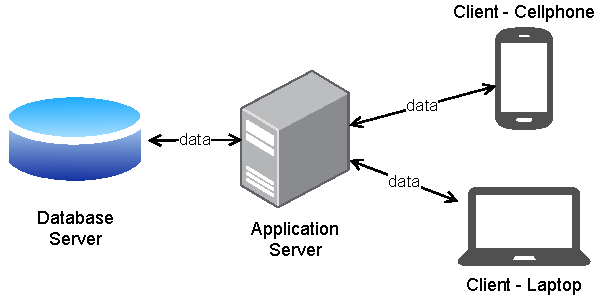
\includegraphics[width=\textwidth]{../images/client-server-3-tier}
\caption{Skema dari 3-tier client-server arsitektur.}
\label{fig:client-server-schema}
\end{figure}

\subsection{Kelebihan dan Kekurangan}
Berikut adalah kelebihan dan kekurangan arsitektur client-server:

\subsubsection{Kelebihan}
Keuntungan dari menerapkan arsitektur client-server adalah:
\begin{itemize}
\item Kemampuan komputasi (dan penyimpanan data) dapat diakses dari berbagai lokasi berjauhan dan oleh banyak komputer/pengguna.
\item Komputasi-komputasi yang membutuhkan kinerja tinggi dapat didelegasikan ke server.
\item Data dapat disentralisasikan sehingga meningkatkan konsistensi data dan mengurangi duplikasi data.
\item  Sistem dapat menerapkan \textit{horizontal scaling }untuk skalabilitas. Horizontal scaling adalah meningkatkan kinerja komputer dengan penambahan komputer agar beban komputasi dibagi ke komputer-komputer yang tersedia. Misalnya, awalnya terdapat 10 000 requests perhari yang ditangani oleh suatu \textit{application server}. Jika \textit{application server} ditambah, maka beban tersebut dibagi di antara kedua \textit{server} tersebut. Vertical scaling adalah meningkat kinerja suatu komputer dengan menaikkan spefikasi komputer tersebut, misalnya dengan menggunakan prosesor yang lebih cepat atau meningkatkan kapasitas memori.
\end{itemize}

\subsubsection{Kekurangan}
Konsekuensi dari penerapan arsitektur client-server adalah sistem jadi lebih kompleks untuk dikelola:
\begin{itemize}
\item Biaya akan meningkat karena terdapat komponen/mesin tambahan yang perlu dikelola.
\item Faktor keamanan juga perlu diperhatikan karena server dan client beroperasi dalam suatu jaringan komputer yang mana rawan terhadap \textit{cyber attack}.
\item Perlunya koordinasi antar-komputer, misalnya komunikasi sinkron dan asinkron serta komputasi parallel.
\item Kompatibilitas antara \textit{server} dan \textit{client} maupun sesama klien.
\item Masalah-masalah yang umum terdapat pada jaringan komputer etwork problems, misalnya \textit{network latency}, kesalahan dalam konfigurasi jaringan, dsb.
\end{itemize}

\section{Contoh Kasus}

\subsection{Deskripsi}
Proyek \textbf{Currency Server} adalah aplikasi berbasis Spring Boot yang berfungsi sebagai layanan backend untuk konversi mata uang. Aplikasi ini menyediakan API REST yang memungkinkan pengguna menambahkan nilai tukar antar mata uang dan melakukan konversi berdasarkan data yang tersedia dalam basis data. Sistem ini menggunakan Spring Data JPA untuk mengelola data dengan MySQL sebagai sistem manajemen basis data. Nilai tukar disimpan dalam entitas yang memiliki kunci komposit, sehingga setiap pasangan mata uang unik dapat dicatat secara akurat. 

Proyek \textbf{Currency Desktop} adalah aplikasi berbasis Java Swing yang berfungsi sebagai antarmuka pengguna untuk layanan konversi mata uang. Aplikasi ini memungkinkan pengguna memilih mata uang asal dan tujuan, memasukkan jumlah yang akan dikonversi, dan mendapatkan hasil konversi melalui integrasi dengan \textbf{Currency Server}. Permintaan data dikirimkan menggunakan koneksi HTTP, dan hasil yang dikembalikan dalam format JSON diproses menggunakan pustaka \textit{Jackson}. Dengan desain berbasis GUI, aplikasi ini memberikan pengalaman pengguna yang lebih interaktif dibandingkan dengan penggunaan API secara langsung.

Kedua proyek ini dirancang untuk bekerja secara terintegrasi, di mana \textbf{Currency Desktop} bertindak sebagai klien yang berkomunikasi dengan \textbf{Currency Server} melalui permintaan HTTP. Dengan arsitektur berbasis layanan ini, sistem dapat dikembangkan lebih lanjut untuk mendukung lebih banyak mata uang, memperluas cakupan API, atau bahkan mengintegrasikan data dari sumber eksternal lainnya.

\subsection{Server}

\subsubsection{Prasyarat}
Sebelum mengatur proyek Maven, pastikan perangkat lunak berikut telah terinstal di sistem Anda:

\begin{itemize}
\item \textbf{Java Development Kit (JDK) 11} (atau versi yang kompatibel)
\item \textbf{Apache Maven} (versi terbaru direkomendasikan)
\item \textbf{MySQL Server} (jika ingin menguji konektivitas database secara lokal)
\item \textbf{Spring Boot Dependencies}
\item \textbf{Koneksi Internet} (untuk mengunduh dependensi yang diperlukan dari repositori Maven)
\end{itemize}

\subsubsection{Instalasi Java dan Maven}
Untuk menginstal Java Development Kit (JDK) dan Maven, ikuti langkah-langkah berikut:

\begin{itemize}
\item \textbf{Instalasi Java (JDK 11)}
\begin{lstlisting}[language=bash]
sudo apt update
sudo apt install openjdk-11-jdk
java -version
\end{lstlisting}
Perintah terakhir akan menampilkan versi Java yang terinstal.

\item \textbf{Instalasi Maven}
\begin{lstlisting}[language=bash]
sudo apt update
sudo apt install maven
mvn -version
\end{lstlisting}
Perintah terakhir akan menampilkan versi Maven yang terinstal.
\end{itemize}

\subsubsection{Membuat Proyek Maven}
Untuk membuat proyek Maven baru, gunakan perintah berikut:

\begin{lstlisting}[language=bash]
mvn archetype:generate -DgroupId=pradita.softwarearchitecture -DartifactId=currency-server -DarchetypeArtifactId=maven-archetype-quickstart -DinteractiveMode=false
\end{lstlisting}

Perintah ini akan menghasilkan struktur proyek Maven dasar. Namun, konfigurasi default perlu dimodifikasi agar sesuai dengan `pom.xml` yang diberikan.

\subsubsection{Mengganti `pom.xml` Default}
Gantilah `pom.xml` yang dihasilkan dengan konten yang telah disediakan. `pom.xml` yang diberikan mencakup:

\begin{itemize}
\item \textbf{Spring Boot dependencies} (`spring-boot-starter-web`, `spring-boot-starter-data-jpa`)
\item \textbf{JUnit untuk pengujian}
\item \textbf{MySQL JDBC Connector} untuk konektivitas database
\item \textbf{Plugin Management untuk siklus hidup build Maven}
\end{itemize}

\subsubsection{Memahami Konfigurasi `pom.xml`}

\begin{itemize}
\item \textbf{Parent POM:}
\begin{lstlisting}[language=xml]
<parent>
<groupId>org.springframework.boot</groupId>
<artifactId>spring-boot-starter-parent</artifactId>
<version>2.7.8</version>
</parent>
\end{lstlisting}
Parent ini mewarisi konfigurasi dari `spring-boot-starter-parent`, yang menyederhanakan manajemen dependensi dan menyediakan konfigurasi default untuk plugin.

\item \textbf{Dependensi:}
\begin{itemize}
\item \textbf{JUnit (`test` scope)} untuk pengujian unit
\item \textbf{Spring Boot Web Starter} (`spring-boot-starter-web`) untuk membuat REST API
\item \textbf{Spring Boot JPA Starter} (`spring-boot-starter-data-jpa`) untuk interaksi database
\item \textbf{MySQL Connector} (`mysql-connector-java`) untuk konektivitas database MySQL
\end{itemize}

\item \textbf{Build Plugins:}
Bagian `<pluginManagement>` mendefinisikan plugin build Maven yang diperlukan untuk memastikan versi yang konsisten. Ini mencakup:
\begin{itemize}
\item \textbf{`maven-compiler-plugin`} (untuk mengatur versi Java ke 11)
\item \textbf{`maven-surefire-plugin`} (untuk menjalankan pengujian unit)
\item \textbf{`maven-jar-plugin`} (untuk mengemas proyek sebagai file JAR)
\item \textbf{`maven-deploy-plugin`} (untuk mendistribusikan artefak)
\end{itemize}
\end{itemize}

\subsubsection{Menambahkan Konfigurasi Tambahan}
Selain `pom.xml`, proyek memerlukan konfigurasi tambahan:

\begin{itemize}
\item \textbf{`application.properties` (Konfigurasi Spring Boot):}
Buat file `src/main/resources/application.properties` dan tambahkan konfigurasi berikut:

\begin{lstlisting}[language=ini]
spring.jpa.hibernate.ddl-auto=create-drop
spring.datasource.url=jdbc:mysql://localhost:3306/currency
spring.datasource.username=alfa
spring.datasource.password=1234
spring.datasource.driver-class-name=com.mysql.cj.jdbc.Driver
spring.jpa.show-sql=true
spring.jpa.defer-datasource-initialization=true
spring.sql.init.mode=always
\end{lstlisting}

Konfigurasi ini memastikan bahwa database `currency` dibuat ulang setiap kali aplikasi dijalankan, menggunakan MySQL sebagai database utama dengan kredensial yang telah disesuaikan.
\end{itemize}


\subsubsection{Membangun dan Menjalankan Proyek}
Setelah struktur proyek dikonfigurasi, jalankan perintah berikut:

\begin{itemize}
\item \textbf{Untuk membangun proyek:}
\begin{lstlisting}[language=bash]
mvn clean package
\end{lstlisting}

\item \textbf{Untuk menjalankan proyek:}
\begin{lstlisting}[language=bash]
mvn spring-boot:run
\end{lstlisting}

Perintah ini akan memulai aplikasi Spring Boot dan mengekspos API yang telah didefinisikan dalam proyek.
\end{itemize}

\subsubsection{Memverifikasi Setup}
Setelah aplikasi berjalan, verifikasi dengan mengakses:

\begin{lstlisting}
http://localhost:8080/
\end{lstlisting}

Jika semuanya telah dikonfigurasi dengan benar, aplikasi Spring Boot akan berjalan dengan sukses.


\subsubsection{Membuat File \texttt{RateId.java}}
Buatlah file `RateId.java` di dalam direktori `src/main/java/pradita/softwarearchitecture/chapter02/`. File ini akan digunakan sebagai kunci utama dalam entitas JPA yang memetakan pasangan mata uang.

Ikuti langkah-langkah berikut untuk membuat file `RateId.java`:

\begin{enumerate}
\item Navigasikan ke direktori proyek Anda menggunakan terminal atau file explorer.
\item Buat folder `chapter02` jika belum ada dengan perintah berikut di terminal:

\begin{lstlisting}[language=bash]
mkdir -p src/main/java/pradita/softwarearchitecture/chapter02
\end{lstlisting}

\item Buat file baru dengan nama `RateId.java` menggunakan perintah:

\begin{lstlisting}[language=bash]
touch src/main/java/pradita/softwarearchitecture/chapter02/RateId.java
\end{lstlisting}

\item Buka file tersebut dengan editor pilihan Anda dan salin kode berikut:

\begin{lstlisting}[style=JavaStyle]
package pradita.softwarearchitecture.chapter02;

import java.io.Serializable;

public class RateId implements Serializable {
	private String fromCurrency;
	private String toCurrency;
	
	public String getFromCurrency() {
		return this.fromCurrency;
	}
	
	public void setFromCurrency(String fromCurrency) {
		this.fromCurrency = fromCurrency;
	}
	
	public String getToCurrency() {
		return this.toCurrency;
	}
	
	public void setToCurrency(String toCurrency) {
		this.toCurrency = toCurrency;
	}
}
\end{lstlisting}

\item Simpan perubahan dan pastikan file sudah tersimpan dalam lokasi yang benar.
\end{enumerate}

Setelah file `RateId.java` dibuat, Anda dapat menggunakannya dalam entitas JPA dengan anotasi `@IdClass` atau `@Embeddable` untuk mengelola kunci komposit dalam basis data.


\subsubsection{Membuat File \texttt{RateRepository.java}}
File `RateRepository.java` perlu dibuat di dalam direktori `src/main/java/pradita/softwarearchitecture/chapter02/`. File ini berfungsi sebagai \textit{repository} dalam Spring Data JPA yang memungkinkan operasi CRUD terhadap entitas `Rate`.

Spring Data JPA menyediakan antarmuka `CrudRepository` yang secara otomatis menangani operasi database tanpa memerlukan implementasi manual. Pada kelas ini, metode \texttt{findFirstByFromCurrencyAndToCurrency} digunakan untuk melakukan pencarian data berdasarkan pasangan mata uang yang diberikan.

\textbf{Langkah-langkah Membuat File \texttt{RateRepository.java}:}

\begin{enumerate}
\item Buka terminal atau file explorer dan navigasikan ke direktori proyek.
\item Jika folder `chapter02` belum ada, buat dengan perintah berikut:

\begin{lstlisting}[language=bash]
mkdir -p src/main/java/pradita/softwarearchitecture/chapter02
\end{lstlisting}

\item Buat file baru dengan nama `RateRepository.java` menggunakan perintah:

\begin{lstlisting}[language=bash]
touch src/main/java/pradita/softwarearchitecture/chapter02/RateRepository.java
\end{lstlisting}

\item Buka file dengan editor pilihan dan masukkan kode berikut:

\begin{lstlisting}[style=JavaStyle]
package pradita.softwarearchitecture.chapter02;

import java.util.Collection;
import org.springframework.data.repository.CrudRepository;

public interface RateRepository extends CrudRepository<Rate, Integer> {
	
	// JPQL Query (dikomentari untuk referensi)
	//@Query("SELECT r FROM Rate r WHERE r.fromCurrency = ?1 and r.toCurrency = ?2")
	
	// Metode ini mencari data berdasarkan pasangan mata uang fromCurrency dan toCurrency.
	Collection<Rate> findFirstByFromCurrencyAndToCurrency(String fromCurrency, String toCurrency);
}
\end{lstlisting}

\item Simpan perubahan dan pastikan file tersimpan dalam lokasi yang benar.
\end{enumerate}

\subsubsection{Penjelasan Kode}
\begin{itemize}
\item \textbf{Paket:} Kelas ini berada dalam paket `pradita.softwarearchitecture.chapter02`, yang menunjukkan bahwa ini merupakan bagian dari struktur proyek.
\item \textbf{Antarmuka \texttt{CrudRepository}:} 
\begin{itemize}
\item `RateRepository` memperluas `CrudRepository<Rate, Integer>`, yang menyediakan operasi dasar seperti `save`, `findById`, `findAll`, dan `delete` tanpa implementasi manual.
\item `Rate` adalah entitas yang dikelola, sedangkan `Integer` adalah tipe data dari kunci utama entitas `Rate`.
\end{itemize}
\item \textbf{Metode Kustom:}
\begin{itemize}
\item \texttt{findFirstByFromCurrencyAndToCurrency}:  
\begin{itemize}
	\item Metode ini secara otomatis diterjemahkan oleh Spring Data JPA menjadi kueri database yang mencari \textbf{data pertama} berdasarkan mata uang asal (`fromCurrency`) dan mata uang tujuan (`toCurrency`).
	\item Jika metode ini digunakan tanpa anotasi `@Query`, Spring Data JPA akan menerjemahkannya ke dalam sintaks SQL atau JPQL secara otomatis.
\end{itemize}
\end{itemize}
\end{itemize}

Setelah file `RateRepository.java` dibuat, penggunaannya dalam layanan Spring Boot memungkinkan pengambilan data berdasarkan pasangan mata uang dengan efisiensi tinggi menggunakan fitur bawaan dari Spring Data JPA.


\subsubsection{Membuat File \texttt{Rate.java}}
File `Rate.java` perlu dibuat di dalam direktori `src/main/java/pradita/softwarearchitecture/chapter02/`. File ini berfungsi sebagai entitas dalam JPA yang merepresentasikan data nilai tukar mata uang dengan menggunakan kunci komposit.

Spring Data JPA menyediakan anotasi `@Entity` untuk menandai kelas ini sebagai entitas yang akan dipetakan ke dalam tabel database. Anotasi `@IdClass(RateId.class)` digunakan untuk menentukan bahwa entitas ini memiliki kunci komposit yang terdiri dari dua atribut: `fromCurrency` dan `toCurrency`.

\textbf{Langkah-langkah Membuat File \texttt{Rate.java}:}

\begin{enumerate}
\item Buka terminal atau file explorer dan navigasikan ke direktori proyek.
\item Jika folder `chapter02` belum ada, buat dengan perintah berikut:

\begin{lstlisting}[language=bash]
mkdir -p src/main/java/pradita/softwarearchitecture/chapter02
\end{lstlisting}

\item Buat file baru dengan nama `Rate.java` menggunakan perintah:

\begin{lstlisting}[language=bash]
touch src/main/java/pradita/softwarearchitecture/chapter02/Rate.java
\end{lstlisting}

\item Buka file dengan editor pilihan dan masukkan kode berikut:

\begin{lstlisting}[style=JavaStyle]
package pradita.softwarearchitecture.chapter02;

import javax.persistence.Entity;
import javax.persistence.Id;
import javax.persistence.IdClass;

@Entity
@IdClass(RateId.class)
public class Rate {
	
	@Id
	private String fromCurrency;
	@Id
	private String toCurrency;
	private Double rate;
	
	Rate(){
		super();
	}
	
	Rate(String fromCurrency, String toCurrency, Double rate) {
		super();
		this.fromCurrency = fromCurrency;
		this.toCurrency = toCurrency;
		this.rate = rate;
	}
	
	public String getFromCurrency() {
		return this.fromCurrency;
	}
	
	public void setFromCurrency(String fromCurrency) {
		this.fromCurrency = fromCurrency;
	}
	
	public String getToCurrency() {
		return this.toCurrency;
	}
	
	public void setToCurrency(String toCurrency) {
		this.toCurrency = toCurrency;
	}
	
	public Double getRate() {
		return this.rate;
	}
	
	public void setRate(Double rate) {
		this.rate = rate;
	}
}
\end{lstlisting}

\item Simpan perubahan dan pastikan file tersimpan dalam lokasi yang benar.
\end{enumerate}

\subsubsection{Penjelasan Kode}
\begin{itemize}
\item \textbf{Paket:} Kelas ini berada dalam paket `pradita.softwarearchitecture.chapter02`, yang menunjukkan bahwa ini merupakan bagian dari struktur proyek.
\item \textbf{Anotasi JPA:}
\begin{itemize}
\item `@Entity` digunakan untuk menandai kelas ini sebagai entitas yang akan dipetakan ke tabel dalam database.
\item `@IdClass(RateId.class)` menunjukkan bahwa kelas ini menggunakan kunci komposit yang didefinisikan dalam kelas `RateId`.
\item `@Id` diberikan pada atribut `fromCurrency` dan `toCurrency`, yang berarti kedua atribut ini membentuk kunci utama entitas `Rate`.
\end{itemize}
\item \textbf{Atribut:}
\begin{itemize}
\item `fromCurrency` - Mewakili mata uang asal dalam pasangan nilai tukar.
\item `toCurrency` - Mewakili mata uang tujuan dalam pasangan nilai tukar.
\item `rate` - Menyimpan nilai tukar antara dua mata uang yang diberikan.
\end{itemize}
\item \textbf{Konstruktor:}
\begin{itemize}
\item Konstruktor tanpa parameter (`Rate()`) diperlukan oleh JPA agar dapat membuat instance objek secara otomatis.
\item Konstruktor dengan parameter digunakan untuk menginisialisasi objek `Rate` dengan nilai `fromCurrency`, `toCurrency`, dan `rate`.
\end{itemize}
\item \textbf{Metode Getter dan Setter:}
\begin{itemize}
\item Metode `getFromCurrency()` dan `setFromCurrency()` digunakan untuk mendapatkan dan mengubah nilai mata uang asal.
\item Metode `getToCurrency()` dan `setToCurrency()` digunakan untuk mendapatkan dan mengubah nilai mata uang tujuan.
\item Metode `getRate()` dan `setRate()` digunakan untuk mendapatkan dan mengubah nilai tukar.
\end{itemize}
\end{itemize}

Setelah file `Rate.java` dibuat, kelas ini dapat digunakan dalam kombinasi dengan repository JPA untuk menyimpan dan mengambil data nilai tukar mata uang dalam basis data secara otomatis.

\subsubsection{Membuat File \texttt{App.java}}
File `App.java` perlu dibuat di dalam direktori `src/main/java/pradita/softwarearchitecture/chapter02/`. File ini berfungsi sebagai kelas utama dalam aplikasi Spring Boot yang menyediakan endpoint REST untuk menambahkan dan mengonversi nilai tukar mata uang.

Spring Boot menyediakan anotasi `@SpringBootApplication` untuk mengonfigurasi aplikasi secara otomatis, sementara anotasi `@RestController` memungkinkan kelas ini menangani permintaan HTTP dan memberikan respons dalam format JSON.

\textbf{Langkah-langkah Membuat File \texttt{App.java}:}

\begin{enumerate}
\item Buka terminal atau file explorer dan navigasikan ke direktori proyek.
\item Jika folder `chapter02` belum ada, buat dengan perintah berikut:

\begin{lstlisting}[language=bash]
mkdir -p src/main/java/pradita/softwarearchitecture/chapter02
\end{lstlisting}

\item Buat file baru dengan nama `App.java` menggunakan perintah:

\begin{lstlisting}[language=bash]
touch src/main/java/pradita/softwarearchitecture/chapter02/App.java
\end{lstlisting}

\item Buka file dengan editor pilihan dan masukkan kode berikut:

\begin{lstlisting}[style=JavaStyle]
package pradita.softwarearchitecture.chapter02;

import java.util.Collection;
import java.util.HashMap;
import java.util.Map;

import org.springframework.beans.factory.annotation.Autowired;
import org.springframework.boot.SpringApplication;
import org.springframework.boot.autoconfigure.SpringBootApplication;
import org.springframework.http.MediaType;
import org.springframework.web.bind.annotation.RequestMapping;
import org.springframework.web.bind.annotation.RestController;

@RestController
@SpringBootApplication
public class App {
	
	@Autowired
	private RateRepository rateRepository;
	
	public static void main(String[] args) {
		SpringApplication.run(App.class, args);
	}
	
	@RequestMapping("/")
	String home() {
		return "Hello World!";
	}
	
	@RequestMapping(path = "/addrate", produces = MediaType.APPLICATION_JSON_VALUE)
	Rate addRate(String from, String to, Double rate) {
		Rate r = new Rate(from, to, rate);
		rateRepository.save(r);
		return r;
	}
	
	@RequestMapping(path = "/convert", produces = MediaType.APPLICATION_JSON_VALUE)
	Map<String, Object> convert(Double value, String from, String to) {
		Map<String, Object> result = new HashMap<>();
		result.put("fromCurrency", from);
		result.put("toCurrency", to);
		Double rate = 0d;
		Collection<Rate> rates = rateRepository.findFirstByFromCurrencyAndToCurrency(from, to);
		if (rates.size() > 0) {
			Rate r = rates.iterator().next();
			rate = r.getRate();
		}
		result.put("rate", rate);
		result.put("value", rate * value);
		return result;
	}
}
\end{lstlisting}

\item Simpan perubahan dan pastikan file tersimpan dalam lokasi yang benar.
\end{enumerate}

\subsubsection{Penjelasan Kode}
\begin{itemize}
\item \textbf{Paket:} Kelas ini berada dalam paket `pradita.softwarearchitecture.chapter02`, yang menunjukkan bahwa ini merupakan bagian dari struktur proyek.
\item \textbf{Anotasi Spring Boot:}
\begin{itemize}
\item `@SpringBootApplication` digunakan untuk mengonfigurasi aplikasi Spring Boot secara otomatis.
\item `@RestController` memungkinkan kelas ini menangani permintaan HTTP dan memberikan respons dalam format JSON.
\end{itemize}
\item \textbf{Atribut:}
\begin{itemize}
\item `rateRepository` adalah objek `RateRepository` yang digunakan untuk mengakses data nilai tukar mata uang dalam basis data.
\end{itemize}
\item \textbf{Metode:}
\begin{itemize}
\item \texttt{main(String[] args)}: 
\begin{itemize}
	\item Metode utama yang menjalankan aplikasi Spring Boot dengan `SpringApplication.run(App.class, args)`.
\end{itemize}
\item \texttt{home()}: 
\begin{itemize}
	\item Endpoint `"/"` yang mengembalikan teks `"Hello World!"` ketika diakses.
\end{itemize}
\item \texttt{addRate(String from, String to, Double rate)}:
\begin{itemize}
	\item Menyediakan endpoint `"/addrate"` untuk menambahkan nilai tukar mata uang baru ke dalam database.
	\item Parameter `from`, `to`, dan `rate` dikonversi menjadi objek `Rate` yang kemudian disimpan ke dalam database melalui `rateRepository.save(r)`.
\end{itemize}
\item \texttt{convert(Double value, String from, String to)}:
\begin{itemize}
	\item Menyediakan endpoint `"/convert"` untuk mengonversi mata uang berdasarkan nilai tukar yang tersimpan di database.
	\item Melakukan pencarian nilai tukar dengan metode `findFirstByFromCurrencyAndToCurrency(from, to)`.
	\item Jika nilai tukar ditemukan, hasil konversi dihitung dan dikembalikan dalam bentuk JSON.
\end{itemize}
\end{itemize}
\end{itemize}

Setelah file `App.java` dibuat, kelas ini akan menjadi titik masuk utama untuk menjalankan aplikasi Spring Boot serta menyediakan layanan REST API untuk menambahkan dan mengonversi nilai tukar mata uang.

\subsection{Dekstop Client}

\subsubsection{Menyiapkan Proyek Maven untuk \texttt{currency-desktop}}
Proyek \texttt{currency-desktop} merupakan aplikasi berbasis Java yang menggunakan Maven sebagai manajer proyek dan pustaka. Konfigurasi yang diberikan dalam berkas `pom.xml` menentukan dependensi yang dibutuhkan serta pengaturan kompilasi proyek.

\textbf{Langkah-langkah Menyiapkan Proyek:}

\begin{enumerate}
\item Buka terminal atau file explorer dan navigasikan ke direktori tempat proyek akan dibuat.
\item Gunakan perintah berikut untuk membuat proyek Maven baru:

\begin{lstlisting}[language=bash]
mvn archetype:generate -DgroupId=pradita.softwarearchitecture -DartifactId=currency-desktop -DarchetypeArtifactId=maven-archetype-quickstart -DinteractiveMode=false
\end{lstlisting}

\item Gantilah berkas `pom.xml` yang dihasilkan dengan konfigurasi berikut:

\begin{lstlisting}[language=xml]
<?xml version="1.0" encoding="UTF-8"?>

<project xmlns="http://maven.apache.org/POM/4.0.0"
xmlns:xsi="http://www.w3.org/2001/XMLSchema-instance" xsi:schemaLocation="http://maven.apache.org/POM/4.0.0 http://maven.apache.org/xsd/maven-4.0.0.xsd">
<modelVersion>4.0.0</modelVersion>

<groupId>pradita.softwarearchitecture</groupId>
<artifactId>currency-desktop</artifactId>
<version>1.0-SNAPSHOT</version>

<name>currency-desktop</name>
<url>http://www.example.com</url>

<properties>
<project.build.sourceEncoding>UTF-8</project.build.sourceEncoding>
<maven.compiler.source>11</maven.compiler.source>
<maven.compiler.target>11</maven.compiler.target>
</properties>

<dependencies>
<dependency>
<groupId>junit</groupId>
<artifactId>junit</artifactId>
<version>4.11</version>
<scope>test</scope>
</dependency>
<dependency>
<groupId>com.fasterxml.jackson.core</groupId>
<artifactId>jackson-core</artifactId>
<version>2.14.2</version>
</dependency>
<dependency>
<groupId>com.fasterxml.jackson.core</groupId>
<artifactId>jackson-databind</artifactId>
<version>2.14.2</version>
</dependency>
</dependencies>

<build>
<pluginManagement>
<plugins>
<plugin>
<artifactId>maven-clean-plugin</artifactId>
<version>3.1.0</version>
</plugin>
<plugin>
<artifactId>maven-resources-plugin</artifactId>
<version>3.0.2</version>
</plugin>
<plugin>
<artifactId>maven-compiler-plugin</artifactId>
<version>3.8.0</version>
</plugin>
<plugin>
<artifactId>maven-surefire-plugin</artifactId>
<version>2.22.1</version>
</plugin>
<plugin>
<artifactId>maven-jar-plugin</artifactId>
<version>3.0.2</version>
</plugin>
<plugin>
<artifactId>maven-install-plugin</artifactId>
<version>2.5.2</version>
</plugin>
<plugin>
<artifactId>maven-deploy-plugin</artifactId>
<version>2.8.2</version>
</plugin>
<plugin>
<artifactId>maven-site-plugin</artifactId>
<version>3.7.1</version>
</plugin>
<plugin>
<artifactId>maven-project-info-reports-plugin</artifactId>
<version>3.0.0</version>
</plugin>
</plugins>
</pluginManagement>
</build>
</project>
\end{lstlisting}

\item Simpan perubahan dan pastikan `pom.xml` sudah dikonfigurasi dengan benar.
\end{enumerate}

\subsubsection{Penjelasan Konfigurasi}
\begin{itemize}
\item \textbf{Grup dan Artefak:}  
\begin{itemize}
\item `groupId`: \texttt{pradita.softwarearchitecture} - Menentukan nama grup proyek.
\item `artifactId`: \texttt{currency-desktop} - Menentukan nama proyek.
\item `version`: `1.0-SNAPSHOT` - Menentukan versi proyek.
\end{itemize}
\item \textbf{Properti Maven:}
\begin{itemize}
\item `maven.compiler.source` dan `maven.compiler.target` diatur ke `11`, menunjukkan bahwa proyek dikompilasi menggunakan Java 11.
\end{itemize}
\item \textbf{Dependensi:}
\begin{itemize}
\item `junit` - Digunakan untuk menjalankan pengujian unit.
\item `jackson-core` - Pustaka untuk memproses JSON dalam Java.
\item `jackson-databind` - Pustaka untuk serialisasi dan deserialisasi objek Java ke JSON.
\end{itemize}
\item \textbf{Pengelolaan Plugin:}
\begin{itemize}
\item `maven-clean-plugin` - Membersihkan artefak build sebelum memulai proses baru.
\item `maven-compiler-plugin` - Mengompilasi kode sumber proyek.
\item `maven-jar-plugin` - Menghasilkan file \texttt{.jar} dari proyek.
\item `maven-surefire-plugin` - Menjalankan pengujian unit secara otomatis.
\item `maven-install-plugin` - Menginstal artefak ke lokal repository.
\item `maven-deploy-plugin` - Mengunggah artefak ke repository eksternal.
\item `maven-site-plugin` - Menghasilkan dokumentasi proyek berbasis situs.
\item `maven-project-info-reports-plugin` - Menyediakan laporan informasi proyek.
\end{itemize}
\end{itemize}

\subsubsection{Membangun dan Menjalankan Proyek}
Setelah konfigurasi selesai, gunakan perintah berikut untuk membangun dan menjalankan proyek:

\begin{itemize}
\item Untuk membersihkan proyek:
\begin{lstlisting}[language=bash]
mvn clean
\end{lstlisting}

\item Untuk membangun proyek:
\begin{lstlisting}[language=bash]
mvn package
\end{lstlisting}

\item Untuk menjalankan aplikasi:
\begin{lstlisting}[language=bash]
java -jar target/currency-desktop-1.0-SNAPSHOT.jar
\end{lstlisting}
\end{itemize}

Dengan mengikuti langkah-langkah di atas, proyek \texttt{currency-desktop} akan siap untuk dijalankan menggunakan Maven dan Java 11.

\subsubsection{Membuat File \texttt{CurrencyDesktop.java}}
File `CurrencyDesktop.java` perlu dibuat di dalam direktori `src/main/java/pradita/softwarearchitecture/chapter02/`. File ini berfungsi sebagai aplikasi GUI berbasis Swing yang memungkinkan pengguna mengonversi nilai mata uang dengan menghubungkan ke layanan backend.

Aplikasi ini menggunakan `JFrame` dan komponen Swing lainnya untuk membangun antarmuka pengguna yang interaktif. Proses konversi dilakukan dengan mengirimkan permintaan HTTP ke server yang menjalankan layanan konversi mata uang.

\textbf{Langkah-langkah Membuat File \texttt{CurrencyDesktop.java}:}

\begin{enumerate}
\item Buka terminal atau file explorer dan navigasikan ke direktori proyek.
\item Jika folder `chapter02` belum ada, buat dengan perintah berikut:

\begin{lstlisting}[language=bash]
mkdir -p src/main/java/pradita/softwarearchitecture/chapter02
\end{lstlisting}

\item Buat file baru dengan nama `CurrencyDesktop.java` menggunakan perintah:

\begin{lstlisting}[language=bash]
touch src/main/java/pradita/softwarearchitecture/chapter02/CurrencyDesktop.java
\end{lstlisting}

\item Buka file dengan editor pilihan dan masukkan kode berikut:

\begin{lstlisting}[style=JavaStyle]
package pradita.softwarearchitecture.chapter02;

import java.awt.Point;
import java.awt.GraphicsEnvironment;
import java.awt.EventQueue;
import java.awt.Font;
import java.awt.event.ActionEvent;
import java.awt.event.ActionListener;
import java.io.BufferedReader;
import java.io.IOException;
import java.io.InputStream;
import java.io.InputStreamReader;
import java.io.UnsupportedEncodingException;
import java.net.HttpURLConnection;
import java.net.URL;
import java.net.URLEncoder;
import java.util.HashMap;
import java.util.Map;

import javax.swing.*;

import com.fasterxml.jackson.databind.JsonNode;
import com.fasterxml.jackson.databind.ObjectMapper;

public class CurrencyDesktop extends JFrame {
	
	private static final long serialVersionUID = 1L;
	private JPanel contentPane;
	private JTextField textFieldValue;
	
	public static void main(String[] args) {
		EventQueue.invokeLater(new Runnable() {
			public void run() {
				try {
					CurrencyDesktop frame = new CurrencyDesktop();
					frame.setVisible(true);
				} catch (Exception e) {
					e.printStackTrace();
				}
			}
		});
	}
	
	public CurrencyDesktop() {
		setTitle("Currency Converter");
		setDefaultCloseOperation(JFrame.EXIT_ON_CLOSE);
		setBounds(100, 100, 493, 130);
		contentPane = new JPanel();
		contentPane.setBorder(new EmptyBorder(5, 5, 5, 5));
		setContentPane(contentPane);
		contentPane.setLayout(null);
		
		Point centerPoint = GraphicsEnvironment.getLocalGraphicsEnvironment().getCenterPoint();
		this.setLocation(centerPoint.x - (int) this.getSize().getWidth() / 2,
		centerPoint.y - (int) this.getSize().getHeight() / 2);
		
		JLabel labelFrom = new JLabel("From");
		labelFrom.setFont(new Font("SansSerif", Font.PLAIN, 20));
		labelFrom.setBounds(16, 20, 63, 16);
		contentPane.add(labelFrom);
		
		JComboBox<String> comboBoxFrom = new JComboBox<>(new String[] { "USD", "GBP", "JPY" });
		comboBoxFrom.setFont(new Font("SansSerif", Font.PLAIN, 20));
		comboBoxFrom.setBounds(81, 15, 111, 26);
		contentPane.add(comboBoxFrom);
		
		JLabel labelTo = new JLabel("To");
		labelTo.setFont(new Font("SansSerif", Font.PLAIN, 20));
		labelTo.setBounds(16, 53, 63, 16);
		contentPane.add(labelTo);
		
		JComboBox<String> comboBoxTo = new JComboBox<>(new String[] { "IDR", "GBP" });
		comboBoxTo.setFont(new Font("SansSerif", Font.PLAIN, 20));
		comboBoxTo.setBounds(81, 48, 111, 26);
		contentPane.add(comboBoxTo);
		
		textFieldValue = new JTextField("1.0");
		textFieldValue.setHorizontalAlignment(SwingConstants.RIGHT);
		textFieldValue.setFont(new Font("SansSerif", Font.PLAIN, 20));
		textFieldValue.setBounds(204, 14, 112, 28);
		contentPane.add(textFieldValue);
		
		JLabel lblConvertedValue = new JLabel("");
		lblConvertedValue.setFont(new Font("SansSerif", Font.PLAIN, 20));
		lblConvertedValue.setHorizontalAlignment(SwingConstants.RIGHT);
		lblConvertedValue.setBounds(204, 48, 112, 26);
		contentPane.add(lblConvertedValue);
		
		JButton btnConvert = new JButton("Convert");
		btnConvert.setFont(new Font("SansSerif", Font.PLAIN, 20));
		btnConvert.setBounds(322, 14, 132, 27);
		contentPane.add(btnConvert);
		
		btnConvert.addActionListener(new ActionListener() {
			public void actionPerformed(ActionEvent e) {
				try {
					Map<String, String> params = new HashMap<>();
					params.put("from", comboBoxFrom.getSelectedItem().toString());
					params.put("to", comboBoxTo.getSelectedItem().toString());
					params.put("value", textFieldValue.getText());
					String paramString = getParamsString(params);
					String getUrl = "http://localhost:8080/convert?" + paramString;
					double convertedValue = getAmount(getUrl);
					lblConvertedValue.setText(String.valueOf(convertedValue));
				} catch (Exception exception) {
					exception.printStackTrace();
				}
			}
		});
	}
	
	private ObjectMapper mapper = new ObjectMapper();
	
	public double getAmount(String getUrl) throws IOException {
		URL obj = new URL(getUrl);
		HttpURLConnection con = (HttpURLConnection) obj.openConnection();
		con.setRequestProperty("accept", "application/json");
		InputStream inputStream = con.getInputStream();
		BufferedReader in = new BufferedReader(new InputStreamReader(inputStream));
		String inputLine;
		StringBuffer response = new StringBuffer();
		while ((inputLine = in.readLine()) != null) {
			response.append(inputLine);
		}
		in.close();
		con.disconnect();
		
		JsonNode node = mapper.readTree(response.toString());
		return node.get("value").asDouble();
	}
	
	public static String getParamsString(Map<String, String> params) throws UnsupportedEncodingException {
		StringBuilder result = new StringBuilder();
		for (Map.Entry<String, String> entry : params.entrySet()) {
			result.append(URLEncoder.encode(entry.getKey(), "UTF-8"));
			result.append("=");
			result.append(URLEncoder.encode(entry.getValue(), "UTF-8"));
			result.append("&");
		}
		return result.toString();
	}
}
\end{lstlisting}

\item Simpan perubahan dan pastikan file tersimpan dalam lokasi yang benar.
\end{enumerate}

\subsubsection{Penjelasan Kode}
\begin{itemize}
\item \textbf{Paket:} Kelas ini berada dalam paket `pradita.softwarearchitecture.chapter02`.
\item \textbf{Antarmuka Pengguna:}
\begin{itemize}
\item Menggunakan `JFrame` dan komponen Swing seperti `JComboBox`, `JButton`, dan `JLabel` untuk antarmuka pengguna.
\end{itemize}
\item \textbf{Fungsi Konversi:}
\begin{itemize}
\item Menggunakan `HttpURLConnection` untuk mengirim permintaan HTTP ke server dan mendapatkan hasil konversi.
\item `getAmount(String getUrl)` mengambil nilai tukar dari server dan mengembalikannya sebagai `double`.
\end{itemize}
\end{itemize}

Setelah `CurrencyDesktop.java` dibuat, aplikasi ini dapat digunakan sebagai antarmuka desktop untuk mengonversi nilai mata uang.

\subsection{Kesimpulan}

Arsitektur perangkat lunak memainkan peran penting dalam pengembangan sistem yang scalable, dapat diandalkan, dan mudah dikelola. Prinsip-prinsip dan teknik yang digunakan dalam perancangan arsitektur berkontribusi terhadap efisiensi sistem serta kemampuannya dalam menangani perubahan kebutuhan bisnis dan teknologi.

Studi kasus yang telah dibahas menunjukkan dampak langsung dari keputusan arsitektur terhadap keberhasilan dan kegagalan sistem perangkat lunak. Transformasi dari arsitektur monolitik ke mikroservis, kegagalan implementasi sistem yang tidak mempertimbangkan desain arsitektural dengan baik, serta penerapan arsitektur event-driven dalam sistem perbankan adalah beberapa contoh bagaimana arsitektur perangkat lunak mempengaruhi keberlangsungan sebuah sistem.

Arsitektur \textit{Client-Server} merupakan salah satu pendekatan fundamental dalam pengembangan sistem terdistribusi. Dengan membagi peran server sebagai penyedia layanan dan klien sebagai pengguna layanan, pendekatan ini menawarkan fleksibilitas, skalabilitas, serta efisiensi dalam pengelolaan sumber daya. Meskipun memiliki kelebihan dalam pengelolaan data yang terpusat, arsitektur ini juga memiliki tantangan seperti ketersediaan dan performa server.

Sebagai studi kasus, implementasi proyek \textit{Currency Server} dan \textit{Currency Desktop} menggambarkan bagaimana arsitektur client-server diterapkan dalam sistem konversi mata uang. \textit{Currency Server} bertindak sebagai backend yang menyediakan layanan melalui API REST, sedangkan \textit{Currency Desktop} berfungsi sebagai klien yang berinteraksi dengan server untuk mendapatkan data nilai tukar. Integrasi antara kedua sistem ini menunjukkan bagaimana arsitektur client-server dapat mendukung komunikasi antara komponen yang berbeda dalam lingkungan perangkat lunak yang terdistribusi.

Dengan memahami konsep dan penerapan arsitektur perangkat lunak, pengembangan sistem dapat dilakukan dengan lebih terstruktur dan efisien. Pemilihan arsitektur yang tepat berdasarkan kebutuhan sistem akan berkontribusi terhadap keberlanjutan dan keberhasilan implementasi perangkat lunak dalam jangka panjang.

%
\chapter{Arsitektur Container}
%\authors{Alfa Yohannis, Richwen Canady, Desfantio Wuidjaja, Vincenzo Matalino}

\section{Apa Itu Container?}

Container adalah paket perangkat lunak yang ringan, mandiri, dan dapat dieksekusi yang mencakup semua komponen yang diperlukan untuk menjalankan sebuah aplikasi, seperti kode, runtime, alat sistem, pustaka, dan konfigurasi. Berbeda dengan virtualisasi tradisional yang memerlukan sistem operasi terpisah untuk setiap mesin virtual, container berbagi kernel sistem operasi dari host. Pendekatan ini meningkatkan efisiensi, mengurangi overhead, dan mempercepat penerapan aplikasi.

Container menyediakan isolasi proses, memastikan bahwa setiap aplikasi berjalan secara independen meskipun berbagi sumber daya sistem yang sama. Isolasi ini meningkatkan keamanan serta menghilangkan konflik dependensi yang sering terjadi dalam model penerapan aplikasi tradisional. Dengan mengemas semua dependensi yang diperlukan, container menjamin konsistensi lingkungan dari tahap pengembangan hingga produksi.

Penggunaan container mendukung pengembangan aplikasi yang skalabel dan portabel. Karena semua dependensi aplikasi sudah termasuk dalam container, perangkat lunak dapat dijalankan secara konsisten di berbagai lingkungan, termasuk cloud, on-premise, dan infrastruktur hibrida. Hal ini meningkatkan keandalan serta mempercepat siklus pengembangan perangkat lunak.

Adopsi teknologi container telah merevolusi penerapan perangkat lunak modern dengan mendukung arsitektur microservices, di mana aplikasi dipecah menjadi layanan-layanan kecil yang independen. Pendekatan ini meningkatkan pemeliharaan dan skalabilitas, serta mengoptimalkan penggunaan sumber daya. Dibandingkan dengan mesin virtual, container menawarkan waktu startup yang lebih cepat dan konsumsi sumber daya yang lebih rendah, menjadikannya pilihan utama untuk aplikasi berbasis cloud dan pengembangan dengan pendekatan DevOps.

\section{Memahami Docker}

Docker adalah platform populer yang digunakan untuk mengembangkan, mendistribusikan, dan menjalankan aplikasi dengan teknologi containerisasi. Dengan Docker, aplikasi dapat dipisahkan dari infrastruktur, sehingga memungkinkan pengiriman perangkat lunak yang lebih cepat dan lebih andal.

Docker menyediakan kemampuan untuk mengemas dan menjalankan aplikasi dalam lingkungan yang terisolasi, yang disebut container. Setiap container mencakup semua dependensi yang diperlukan, seperti pustaka dan konfigurasi, sehingga memastikan aplikasi dapat berjalan secara konsisten di berbagai lingkungan tanpa konflik.

Dengan menggunakan Docker, proses deployment menjadi lebih efisien karena aplikasi dapat dipindahkan dari satu lingkungan ke lingkungan lain tanpa perubahan konfigurasi yang signifikan. Selain itu, Docker memungkinkan pengelolaan sumber daya yang lebih baik dan mendukung pengembangan berbasis microservices, di mana setiap layanan dapat dijalankan secara independen dalam container yang terpisah.




\section{Perbandingan Container dan Virtual Machine}

\begin{figure}[h]
	\centering
	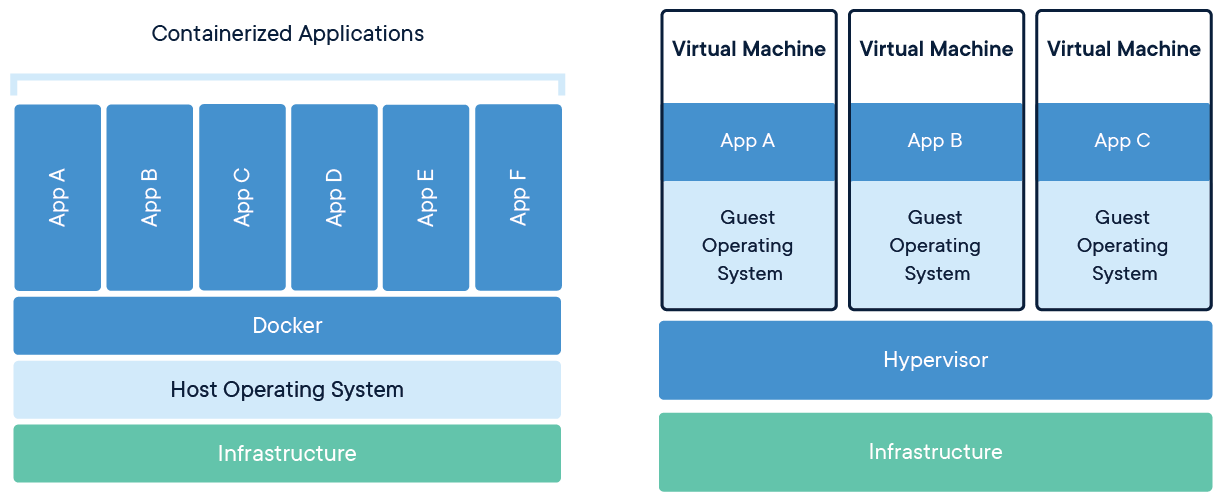
\includegraphics[width=\textwidth]{../images/container-vm.png}
	\caption{Perbedaan antara Container dan Virtual Machine}
	\label{fig:container-vm}
\end{figure}

Virtual machine (VM) dan container merupakan dua teknologi yang digunakan untuk menjalankan aplikasi dalam lingkungan yang terisolasi. Namun, keduanya memiliki pendekatan yang berbeda dalam hal arsitektur dan efisiensi sumber daya.

\subsection{Virtual Machine}
Virtual machine mencakup seluruh sistem operasi, termasuk kernel dan aplikasi, sehingga lebih berat dan membutuhkan lebih banyak sumber daya dibandingkan dengan container. Startup VM cenderung lebih lambat karena sistem operasi perlu dimuat sepenuhnya sebelum aplikasi dapat dijalankan.

VM bergantung pada teknologi \textbf{hypervisor}, yang mengelola beberapa virtual machine di satu mesin fisik dengan mengabstraksi sumber daya perangkat keras. Dengan adanya hypervisor, beberapa sistem operasi dapat berjalan secara independen di atas satu perangkat keras yang sama.

\subsection{Container}
Berbeda dengan VM, container berbagi kernel sistem operasi host, yang membuatnya lebih ringan dan membutuhkan lebih sedikit sumber daya. Karena tidak perlu memuat sistem operasi terpisah, container dapat dimulai lebih cepat dibandingkan dengan VM.

Keunggulan utama container adalah efisiensinya dalam menjalankan aplikasi berbasis microservices dan praktik DevOps. Dengan container, aplikasi dapat diisolasi secara independen tanpa overhead yang besar, memungkinkan pengelolaan dan skalabilitas yang lebih baik dalam lingkungan pengembangan dan produksi.


\section{Docker}

\begin{figure}[h]
	\centering
	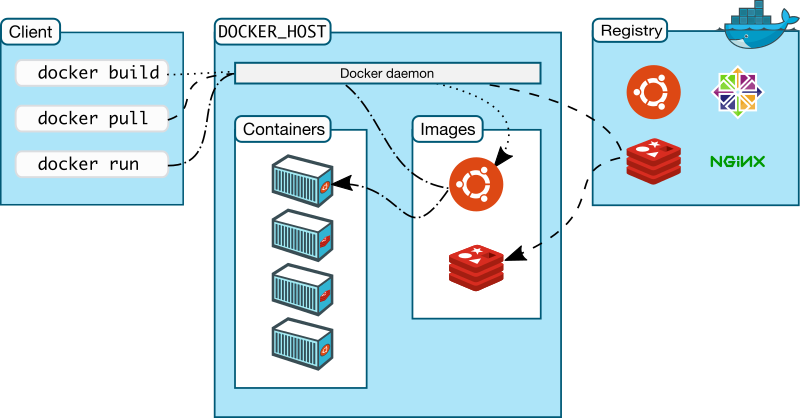
\includegraphics[width=\textwidth]{../images/docker.png}
	\caption{Struktur Docker}
	\label{fig:docker}
\end{figure}

Docker adalah platform yang memungkinkan pembuatan, pengiriman, dan menjalankan aplikasi dalam lingkungan container. Teknologi ini menyederhanakan proses deployment dengan mengisolasi aplikasi beserta dependensinya dalam unit yang ringan dan portabel.

\section{Komponen Docker}

Docker terdiri dari beberapa komponen utama yang bekerja bersama untuk mengelola container.

\subsection{Docker Engine}
Docker Engine adalah inti dari sistem Docker yang bertanggung jawab untuk menjalankan dan mengelola container. Komponen utama dalam Docker Engine meliputi:
\begin{itemize}
	\item \textbf{Docker Daemon}: Berjalan pada mesin host dan bertugas mengelola container, image, jaringan, serta volume penyimpanan.
	\item \textbf{Docker Client}: Antarmuka baris perintah (CLI) yang digunakan untuk berinteraksi dengan Docker Daemon.
\end{itemize}

\subsection{Images}
Image Docker adalah template baca-saja yang digunakan untuk membuat container. Image berisi semua yang dibutuhkan untuk menjalankan aplikasi, termasuk kode, dependensi, serta konfigurasi.

\subsection{Containers}
Container adalah instance yang dapat dijalankan dari image Docker. Container memungkinkan aplikasi berjalan dalam lingkungan yang terisolasi tanpa memerlukan sistem operasi terpisah, sehingga lebih ringan dibandingkan dengan virtual machine.

\subsection{Docker Registry}
Docker Registry adalah tempat penyimpanan image Docker. Salah satu contoh registry yang umum digunakan adalah \textbf{Docker Hub}, yang menyediakan berbagai image yang dapat diunduh dan digunakan sesuai kebutuhan.

Dengan menggunakan komponen-komponen ini, Docker menyediakan solusi yang efisien untuk pengelolaan dan distribusi aplikasi, memungkinkan pengembang untuk membangun lingkungan yang konsisten dari tahap pengembangan hingga produksi.

\section{Keunggulan Penggunaan Container}

Penggunaan container dalam pengelolaan aplikasi menawarkan berbagai keuntungan dibandingkan dengan metode tradisional seperti virtual machine. Beberapa keunggulan utama dari teknologi container adalah sebagai berikut:

\subsection{Portabilitas}
Container memastikan lingkungan aplikasi tetap konsisten di berbagai platform, baik itu di lingkungan pengembangan, pengujian, maupun produksi. Dengan demikian, aplikasi dapat dijalankan di berbagai sistem tanpa perlu konfigurasi ulang.

\subsection{Efisiensi}
Dibandingkan dengan virtual machine, container memiliki overhead yang lebih rendah karena tidak memerlukan sistem operasi terpisah untuk setiap instance. Dengan berbagi kernel sistem operasi host, penggunaan sumber daya menjadi lebih efisien.

\subsection{Skalabilitas}
Container memungkinkan aplikasi untuk dengan mudah disesuaikan berdasarkan permintaan. Dengan teknologi container orchestration seperti Kubernetes, container dapat diperbanyak atau dikurangi secara otomatis sesuai kebutuhan sistem.

\subsection{Isolasi}
Setiap container berjalan dalam lingkungan yang terisolasi, sehingga mencegah konflik antar aplikasi yang berjalan dalam satu sistem. Isolasi ini juga meningkatkan keamanan karena container tidak saling mempengaruhi satu sama lain.

\subsection{CI/CD (Continuous Integration/Continuous Deployment)}
Container mendukung otomatisasi dalam pengembangan perangkat lunak dengan mempermudah proses integrasi, pengujian, dan deployment. Dengan container, pengembang dapat membangun pipeline CI/CD yang lebih cepat dan andal, memungkinkan iterasi perangkat lunak yang lebih efisien.

Dengan keunggulan-keunggulan ini, teknologi container menjadi pilihan utama dalam pengembangan perangkat lunak modern, terutama dalam lingkungan berbasis cloud dan arsitektur microservices.



\section{Kekurangan Penggunaan Container}

Meskipun container menawarkan berbagai keunggulan, terdapat beberapa tantangan yang perlu diperhatikan dalam penggunaannya. Berikut adalah beberapa kekurangan utama dari teknologi container:

\subsection{Keamanan}
Container berbagi kernel sistem operasi host, yang dapat menimbulkan risiko keamanan jika tidak dikonfigurasi dengan benar. Kerentanan dalam satu container berpotensi memengaruhi seluruh sistem, terutama jika isolasi antar container tidak diterapkan dengan baik.

\subsection{Persistensi}
Pengelolaan aplikasi berbasis stateful dalam lingkungan container dapat menjadi tantangan. Karena container bersifat ephemeral (tidak permanen), data yang disimpan di dalamnya dapat hilang saat container dihentikan atau dihapus. Oleh karena itu, diperlukan solusi penyimpanan eksternal seperti volume atau database yang mendukung persistensi data.

\subsection{Jaringan}
Konfigurasi jaringan dalam lingkungan container bisa menjadi kompleks, terutama dalam skenario yang melibatkan banyak container yang harus berkomunikasi satu sama lain. Manajemen jaringan dalam skala besar memerlukan pendekatan yang matang, termasuk penggunaan alat orkestrasi seperti Kubernetes untuk mengelola komunikasi antar container.

\subsection{Kompatibilitas}
Tidak semua aplikasi cocok untuk dijalankan dalam container. Aplikasi yang bergantung langsung pada perangkat keras atau memiliki arsitektur yang sangat monolitik mungkin memerlukan adaptasi tambahan sebelum dapat di-containerisasi dengan baik.

Meskipun memiliki beberapa keterbatasan, teknologi container tetap menjadi pilihan utama dalam banyak skenario pengembangan perangkat lunak. Dengan konfigurasi yang tepat dan strategi mitigasi risiko, kelemahan-kelemahan tersebut dapat diminimalkan untuk memaksimalkan manfaat container dalam pengelolaan aplikasi modern.


\section{Contoh Penerapan Container}

Teknologi container digunakan dalam berbagai skenario untuk meningkatkan efisiensi, skalabilitas, dan konsistensi dalam pengembangan serta pengelolaan aplikasi. Berikut adalah beberapa contoh penerapannya:

\subsection{Aplikasi Web}
Container memungkinkan deployment layanan web dalam lingkungan yang konsisten di berbagai platform. Dengan container, konfigurasi server dan dependensi dapat dikemas dalam satu unit yang mudah didistribusikan dan dijalankan di lingkungan pengembangan, pengujian, maupun produksi.

\subsection{Arsitektur Microservices}
Container sangat mendukung penerapan arsitektur microservices, di mana setiap layanan berjalan secara independen dalam container yang terisolasi. Dengan pendekatan ini, pengelolaan, pemeliharaan, dan penskalaan layanan menjadi lebih fleksibel dan efisien.

\subsection{Lingkungan Pengembangan}
Penggunaan container dalam lingkungan pengembangan memastikan bahwa setiap anggota tim bekerja dalam lingkungan yang seragam. Dengan container, masalah terkait perbedaan sistem operasi atau konfigurasi dapat dihindari, sehingga pengembangan dan pengujian dapat berjalan lebih lancar.

\subsection{Pemrosesan Data}
Container digunakan untuk menjalankan tugas pemrosesan data dalam lingkungan yang terisolasi. Teknologi ini memungkinkan eksekusi pipeline data secara efisien tanpa perlu khawatir tentang konflik dependensi atau perbedaan konfigurasi sistem.

\subsection{Pipeline CI/CD}
Container mendukung otomatisasi dalam siklus pengembangan perangkat lunak dengan memungkinkan penerapan pipeline CI/CD (Continuous Integration/Continuous Deployment). Dengan container, proses build, pengujian, dan deployment dapat dilakukan secara lebih cepat dan konsisten di berbagai lingkungan.

Dengan berbagai penerapan ini, container menjadi solusi utama dalam pengembangan perangkat lunak modern, memungkinkan aplikasi yang lebih modular, fleksibel, dan dapat dijalankan di berbagai infrastruktur tanpa hambatan yang signifikan.


\section{Kesimpulan}

Penggunaan container, terutama dengan Docker, telah merevolusi cara pengembangan dan deployment perangkat lunak. Teknologi ini menyediakan lingkungan yang ringan, konsisten, dan terisolasi, memungkinkan aplikasi dijalankan dengan efisien di berbagai platform tanpa bergantung pada konfigurasi spesifik sistem.

Meskipun terdapat beberapa tantangan dalam penerapan container, keunggulannya sering kali lebih dominan, terutama dalam arsitektur berbasis microservices dan sistem yang memerlukan skalabilitas tinggi. Container memungkinkan pengelolaan aplikasi yang lebih fleksibel, mempercepat siklus pengembangan, serta meningkatkan efisiensi dalam distribusi dan deployment perangkat lunak.

Dengan semakin luasnya adopsi teknologi container, ekosistem pengembangan perangkat lunak terus berkembang menuju solusi yang lebih modular, portabel, dan mudah dikelola, menjadikannya pilihan utama dalam pengelolaan aplikasi modern.



\section{Contoh Aplikasi Container}
\label{sec:contoh_aplikasi_container}

Untuk mendemonstrasikan penggunaan container, berikut adalah contoh sistem yang terdiri dari beberapa \textit{container Docker} yang berjalan secara independen dan berkomunikasi melalui jaringan \texttt{bridge}. Setiap layanan memiliki peran spesifik dalam pengelolaan data karyawan dan performanya, serta menyediakan antarmuka untuk administrasi database. Kode program dapat ditemukan di \url{https://github.com/alfa-yohannis/software-architecture/tree/main/code/chapter02/java-example}.

\begin{figure}[h]
	\centering
	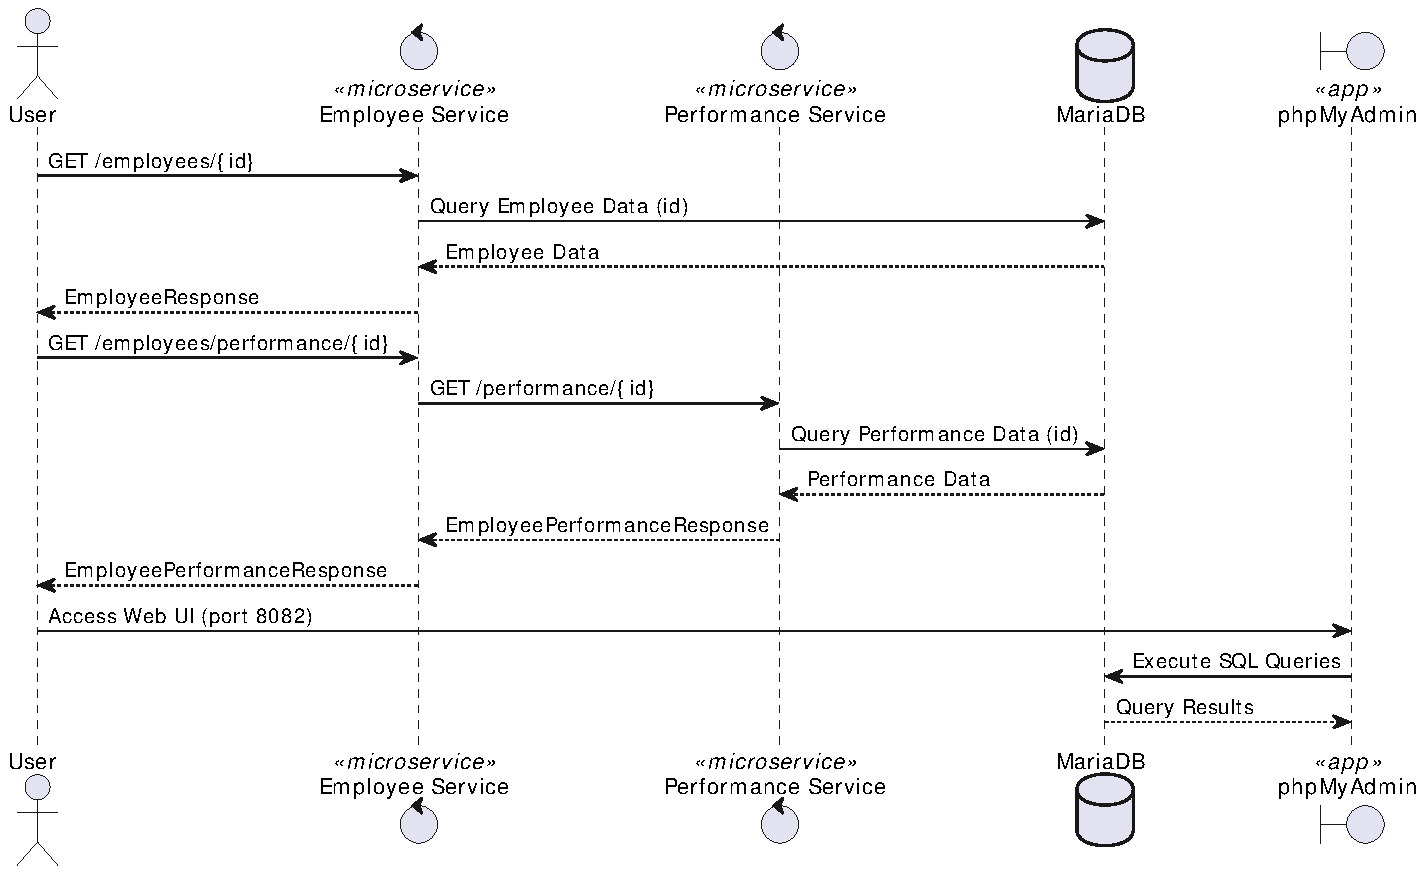
\includegraphics[width=\textwidth]{../images/out/microservices-employees}
	\caption{Struktur Docker}
	\label{fig:employee_performance}
\end{figure}


.

\subsection{Employee Service}

\textit{Employee Service} adalah layanan utama yang bertanggung jawab atas pengelolaan data karyawan. Layanan ini dikategorikan sebagai \textit{microservice} dan berjalan dalam \textit{container Docker} berbasis image \texttt{employee-service}. 

Ketika pengguna mengakses endpoint \texttt{/employees/\{id\}}, Employee Service akan mengirimkan permintaan ke \textit{MariaDB} untuk mengambil data karyawan berdasarkan ID yang diberikan. \textit{MariaDB} kemudian mengembalikan data karyawan yang diminta, yang selanjutnya dikirimkan kembali kepada pengguna dalam format \texttt{EmployeeResponse}. Jika data tidak ditemukan, Employee Service akan merespons dengan \texttt{204 No Content}.

Selain itu, Employee Service juga menangani permintaan terkait performa karyawan. Ketika pengguna meminta data performa dengan \texttt{GET /employees/performance/\{id\}}, Employee Service meneruskan permintaan ke \textit{Performance Service}. \textit{Performance Service} kemudian mengambil data performa dari \textit{MariaDB}, mengolahnya, dan mengembalikannya ke Employee Service dalam format \texttt{EmployeePerformanceResponse}. Employee Service kemudian mengirimkan hasil akhirnya ke pengguna.

\subsection{Performance Service}

\textit{Performance Service} merupakan \textit{microservice} yang bertanggung jawab atas pengelolaan data performa karyawan. Layanan ini berjalan dalam \textit{container Docker} berbasis image \texttt{performance-service} dan memiliki ketergantungan terhadap \textit{MariaDB}.

Ketika Employee Service mengirimkan permintaan terkait performa karyawan ke \textit{Performance Service}, layanan ini akan mencari data performa karyawan yang diminta di \textit{MariaDB}. \textit{MariaDB} mengembalikan hasil query, yang kemudian diproses dan dikembalikan oleh Performance Service ke Employee Service. Hasil akhir akan dikirimkan ke pengguna dalam bentuk \texttt{EmployeePerformanceResponse}.

\subsection{MariaDB}

\textit{MariaDB} merupakan database utama dalam sistem yang bertindak sebagai penyimpanan data bagi \textit{Employee Service} dan \textit{Performance Service}. \textit{Container Docker} yang menjalankan MariaDB menggunakan image \texttt{mariadb:latest}.

Semua data karyawan dan performanya disimpan di \textit{MariaDB}. \textit{Employee Service} dan \textit{Performance Service} melakukan query ke database ini untuk mendapatkan data yang diminta. Selain itu, layanan \textit{phpMyAdmin} juga berinteraksi dengan MariaDB untuk keperluan administrasi database.

\subsection{phpMyAdmin}

\textit{phpMyAdmin} merupakan aplikasi berbasis web yang digunakan untuk mengelola \textit{MariaDB} secara visual. Layanan ini berjalan dalam \textit{container Docker} berbasis image \texttt{phpmyadmin/\-phpmyadmin:\-latest} dan dapat diakses melalui port \texttt{8082}.

Pengguna dapat mengakses \textit{phpMyAdmin} melalui browser untuk mengeksekusi perintah SQL pada \textit{MariaDB}. Ketika pengguna menjalankan query di phpMyAdmin, layanan ini akan meneruskannya ke \textit{MariaDB}. Hasil eksekusi query akan dikembalikan dari \textit{MariaDB} dan ditampilkan dalam antarmuka web phpMyAdmin.


\section{Instalasi dan Pengecekan Docker}

Untuk menjalankan sistem berbasis \textit{container Docker}, langkah pertama adalah memastikan Docker telah terinstal dan berjalan dengan baik di sistem.

\subsection{Instalasi Docker}

Jika Docker belum terinstal, ikuti langkah-langkah berikut:

\begin{enumerate}
\item Unduh dan instal Docker sesuai dengan sistem operasi yang digunakan:
\begin{itemize}
\item Linux (Ubuntu/Debian):
\begin{lstlisting}[language=bash]
sudo apt update
sudo apt install docker.io -y
sudo systemctl enable --now docker
\end{lstlisting}

\item Windows/macOS: Kunjungi \texttt{https://www.docker.com/get-started}. Unduh dan instal Docker Desktop.
\end{itemize}

\item Verifikasi instalasi Docker dengan menjalankan perintah berikut:
\begin{lstlisting}[language=bash]
docker --version
\end{lstlisting}
Jika instalasi berhasil, perintah ini akan menampilkan versi Docker yang terpasang.
\end{enumerate}

\subsection{Mengecek Status Docker}

Untuk memastikan Docker berjalan dengan benar, gunakan perintah berikut:

\begin{lstlisting}[language=bash]
sudo systemctl status docker
\end{lstlisting}

Jika Docker aktif, keluaran perintah ini akan menunjukkan status \texttt{active (running)}. Jika tidak, jalankan perintah berikut untuk memulai Docker:

\begin{lstlisting}[language=bash]
sudo systemctl start docker
\end{lstlisting}

Selain itu, untuk menguji apakah Docker dapat menjalankan container dengan benar, jalankan perintah berikut:

\begin{lstlisting}[language=bash]
docker run hello-world
\end{lstlisting}

Jika Docker berfungsi dengan baik, perintah ini akan menarik dan menjalankan container uji coba yang mencetak pesan konfirmasi ke layar.

\section{Instalasi dan Pengecekan Docker Compose}

Docker Compose digunakan untuk mengelola beberapa container Docker sebagai satu kesatuan dalam sebuah aplikasi. Berikut langkah-langkah untuk menginstal dan memverifikasi Docker Compose.

\subsection{Instalasi Docker Compose}

Jika Docker Compose belum terinstal, ikuti langkah-langkah berikut:

\begin{enumerate}
	\item Unduh dan instal Docker Compose sesuai dengan sistem operasi yang digunakan:
	\begin{itemize}
		\item Linux (Ubuntu/Debian):
		\begin{lstlisting}[language=bash]
			sudo apt update
			sudo apt install docker-compose -y
		\end{lstlisting}
		
		\item Windows/macOS: Docker Compose sudah termasuk dalam Docker Desktop. Kunjungi \texttt{https://www.docker.com/get-started}. Pastikan Docker Desktop telah terinstal dengan mengunduhnya.
	\end{itemize}
	
	\item Verifikasi instalasi Docker Compose dengan menjalankan perintah berikut:
	\begin{lstlisting}[language=bash]
		docker-compose --version
	\end{lstlisting}
	Jika instalasi berhasil, perintah ini akan menampilkan versi Docker Compose yang terpasang.
\end{enumerate}

\subsection{Mengecek Status Docker Compose}

Untuk memastikan Docker Compose dapat berjalan dengan baik, pastikan Docker telah berjalan dan uji coba dengan menjalankan perintah berikut:

\begin{lstlisting}[language=bash]
	docker-compose up -d
\end{lstlisting}

Perintah ini akan menjalankan semua container yang telah didefinisikan dalam file \texttt{docker-compose.yml} secara \textit{detached} (di latar belakang). Untuk melihat daftar container yang sedang berjalan, gunakan:

\begin{lstlisting}[language=bash]
	docker-compose ps
\end{lstlisting}

Jika ingin menghentikan semua container yang berjalan dengan Docker Compose, gunakan perintah berikut:

\begin{lstlisting}[language=bash]
	docker-compose down
\end{lstlisting}

Dengan langkah-langkah di atas, Docker Compose akan siap digunakan untuk mengelola dan mengorkestrasi layanan berbasis container dalam sistem.



\section{Performance Service}

\textit{Performance Service} merupakan layanan yang dikemas dalam \textit{container Docker} dan dikembangkan menggunakan Maven serta Java dengan \textit{Eclipse Temurin JDK 17}. Berikut adalah penjelasan mengenai tahapan pembangunan dan eksekusi layanan ini berdasarkan \texttt{Dockerfile}.

\subsection{Struktur Dockerfile}

Berikut adalah isi \texttt{Dockerfile} yang digunakan untuk membangun dan menjalankan layanan ini:

\begin{lstlisting}[language=docker]
	# STEP 1
	FROM maven:3.9.6-eclipse-temurin-17 as build
	
	WORKDIR /workspace/app
	
	COPY pom.xml .
	COPY src src
	
	RUN mvn install -DskipTests
	RUN mkdir -p target/dependency && (cd target/dependency; jar -xf ../*.jar)
	
	COPY application.properties target/dependency
	
	#STEP 2
	FROM maven:3.9.6-eclipse-temurin-17
	EXPOSE 8081
	#VOLUME /tmp
	ARG DEPENDENCY=/workspace/app/target/dependency
	COPY --from=build ${DEPENDENCY}/BOOT-INF/lib /app/lib
	COPY --from=build ${DEPENDENCY}/META-INF /app/META-INF
	COPY --from=build ${DEPENDENCY}/BOOT-INF/classes /app
	COPY --from=build ${DEPENDENCY}/BOOT-INF/classes /app
	COPY --from=build ${DEPENDENCY}/application.properties /app
	ENTRYPOINT ["java","-cp","app:app/lib/*","software.architecture.microservice.PerformanceServiceApplication"]
\end{lstlisting}

\subsection{Tahapan Pembangunan dan Eksekusi}

\subsubsection{Tahap Build}
Pada tahap ini, digunakan \textit{multi-stage build} untuk membangun aplikasi dan menyalin file yang diperlukan ke dalam container.

\begin{itemize}
	\item \texttt{FROM maven:3.9.6-eclipse-temurin-17 as build} \\
	Menentukan base image yang digunakan untuk proses build, yaitu Maven dengan JDK 17.
	\item \texttt{WORKDIR /workspace/app} \\
	Mengatur direktori kerja dalam container.
	\item \texttt{COPY pom.xml .} dan \texttt{COPY src src} \\
	Menyalin file konfigurasi Maven dan kode sumber ke dalam container.
	\item \texttt{RUN mvn install -DskipTests} \\
	Melakukan proses build menggunakan Maven tanpa menjalankan pengujian.
	\item \texttt{RUN mkdir -p target/dependency} \\
	Membuat direktori untuk menyimpan hasil ekstraksi file JAR.
	\item \texttt{jar -xf ../*.jar} \\
	Mengekstrak isi file JAR untuk mengambil dependensi yang diperlukan.
	\item \texttt{COPY application.properties target/dependency} \\
	Menyalin file konfigurasi ke dalam direktori dependensi.
\end{itemize}

\subsubsection{Tahap Runtime}
Setelah tahap build selesai, container baru dibuat untuk menjalankan layanan.

\begin{itemize}
	\item \texttt{FROM maven:3.9.6-eclipse-temurin-17} \\
	Menggunakan image Maven dengan JDK 17 sebagai base runtime.
	\item \texttt{EXPOSE 8081} \\
	Membuka port 8081 agar layanan dapat diakses.
	\item \texttt{ARG DEPENDENCY=/workspace/app/target/dependency} \\
	Mendefinisikan lokasi direktori dependensi hasil build.
	\item \texttt{COPY --from=build} \\
	Menyalin file hasil build dari tahap sebelumnya ke dalam container runtime.
	\item \texttt{ENTRYPOINT} \\
	Menjalankan aplikasi dengan perintah:
	\begin{lstlisting}[language=bash]
		java -cp app:app/lib/* software.architecture.microservice.PerformanceServiceApplication
	\end{lstlisting}
\end{itemize}

\subsection{Keuntungan Multi-Stage Build}

Pendekatan \textit{multi-stage build} dalam Dockerfile ini memberikan beberapa keuntungan:
\begin{itemize}
	\item Memisahkan proses build dan runtime sehingga image akhir lebih kecil dan efisien.
	\item Menghilangkan kebutuhan untuk menyertakan toolchain build dalam image runtime.
	\item Meningkatkan keamanan dengan hanya menyertakan file yang diperlukan untuk eksekusi.
\end{itemize}

Dengan pendekatan ini, \textit{Performance Service} dapat berjalan secara efisien dalam container dengan ukuran yang lebih ringan tanpa menyertakan lingkungan build Maven yang lengkap.


\section{Employee Service}

\textit{Employee Service} merupakan layanan yang dikemas dalam \textit{container Docker} dan dikembangkan menggunakan Maven serta Java dengan \textit{Eclipse Temurin JDK 17}. Berikut adalah penjelasan mengenai tahapan pembangunan dan eksekusi layanan ini berdasarkan \texttt{Dockerfile}.

\subsection{Struktur Dockerfile}

Berikut adalah isi \texttt{Dockerfile} yang digunakan untuk membangun dan menjalankan layanan ini:

\begin{lstlisting}[language=docker]
	FROM maven:3.9.6-eclipse-temurin-17 as build
	
	WORKDIR /workspace/app
	
	COPY pom.xml .
	COPY src src
	
	RUN mvn install -DskipTests
	RUN mkdir -p target/dependency && (cd target/dependency; jar -xf ../*.jar)
	
	COPY application.properties target/dependency
	
	FROM maven:3.9.6-eclipse-temurin-17
	EXPOSE 8080
	#VOLUME /tmp
	ARG DEPENDENCY=/workspace/app/target/dependency
	COPY --from=build ${DEPENDENCY}/BOOT-INF/lib /app/lib
	COPY --from=build ${DEPENDENCY}/META-INF /app/META-INF
	COPY --from=build ${DEPENDENCY}/BOOT-INF/classes /app
	COPY --from=build ${DEPENDENCY}/BOOT-INF/classes /app
	COPY --from=build ${DEPENDENCY}/application.properties /app
	ENTRYPOINT ["java","-cp","app:app/lib/*","software.architecture.microservice.EmployeeServiceApplication"]
\end{lstlisting}

\subsection{Tahapan Pembangunan dan Eksekusi}

\subsubsection{Tahap Build}
Tahap ini menggunakan strategi \textit{multi-stage build} yang memisahkan proses build dan runtime untuk menghasilkan image yang lebih ringan.

\begin{itemize}
	\item \texttt{FROM maven:3.9.6-eclipse-temurin-17 as build} \\
	Menentukan base image Maven dengan JDK 17 untuk proses build.
	\item \texttt{WORKDIR /workspace/app} \\
	Mengatur direktori kerja di dalam container.
	\item \texttt{COPY pom.xml .} dan \texttt{COPY src src} \\
	Menyalin file konfigurasi Maven serta kode sumber ke dalam container.
	\item \texttt{RUN mvn install -DskipTests} \\
	Melakukan proses build aplikasi menggunakan Maven tanpa menjalankan pengujian.
	\item \texttt{RUN mkdir -p target/dependency} \\
	Membuat direktori penyimpanan hasil ekstraksi file JAR.
	\item \texttt{jar -xf ../*.jar} \\
	Mengekstrak file JAR untuk mendapatkan dependensi yang diperlukan.
	\item \texttt{COPY application.properties target/dependency} \\
	Menyalin file konfigurasi aplikasi ke dalam direktori dependensi.
\end{itemize}

\subsubsection{Tahap Runtime}
Tahap ini menyiapkan lingkungan runtime untuk menjalankan aplikasi.

\begin{itemize}
	\item \texttt{FROM maven:3.9.6-eclipse-temurin-17} \\
	Menggunakan base image Maven dengan JDK 17 untuk lingkungan runtime.
	\item \texttt{EXPOSE 8080} \\
	Membuka port 8080 agar layanan dapat diakses.
	\item \texttt{ARG DEPENDENCY=/workspace/app/target/dependency} \\
	Mendefinisikan lokasi direktori hasil build.
	\item \texttt{COPY --from=build} \\
	Menyalin file hasil build dari tahap sebelumnya ke dalam container runtime.
	\item \texttt{ENTRYPOINT} digunakan untuk menjalankan aplikasi dengan perintah:
	\begin{lstlisting}[language=bash]
		java -cp app:app/lib/* software.architecture.microservice.EmployeeServiceApplication
	\end{lstlisting}
	Perintah ini mengeksekusi aplikasi menggunakan semua dependensi yang sudah disalin ke dalam direktori \texttt{/app}.
\end{itemize}

\subsection{Keuntungan Multi-Stage Build}

Strategi \textit{multi-stage build} yang digunakan dalam Dockerfile ini memberikan beberapa keuntungan:
\begin{itemize}
	\item Memisahkan lingkungan build dan runtime sehingga image lebih kecil.
	\item Menghilangkan dependensi yang tidak diperlukan dalam image runtime.
	\item Meningkatkan keamanan dengan hanya menyertakan file yang diperlukan untuk eksekusi aplikasi.
\end{itemize}

Dengan pendekatan ini, \textit{Employee Service} dapat dijalankan secara efisien dalam container yang lebih ringan tanpa menyertakan seluruh lingkungan build Maven.


\section{Docker Compose Configuration}

\textit{Docker Compose} digunakan untuk mengelola beberapa \textit{container Docker} sebagai satu kesatuan dalam sebuah aplikasi berbasis \textit{microservices}. Berikut adalah penjelasan mengenai konfigurasi layanan menggunakan \texttt{docker-compose.yml}.

\subsection{Struktur Docker Compose}

Berikut adalah isi dari \texttt{docker-compose.yml} yang digunakan untuk menjalankan layanan dalam sistem:

\begin{lstlisting}[language=yaml]
	networks:
		microservices:
		name: microservices
		driver: bridge
	
	services:
	# MariaDB
	mariadb:
		image: mariadb:latest
		container_name: mariadb
		environment:
		- MYSQL_ROOT_PASSWORD=1234
		- MYSQL_USER=alfa
		- MYSQL_PASSWORD=1234
		ports:
		- "3306:3306"
		restart: always
		networks:
		microservices:
		aliases:
		- mariadb
	
	# phpMyAdmin
	phpmyadmin:
		image: phpmyadmin/phpmyadmin:latest
		container_name: phpmyadmin
		ports:
		- "8082:80"
		restart: always
		depends_on:
		- mariadb
		environment:
		PMA_HOST: mariadb
		PMA_PORT: 3306
		networks:
		microservices:
		aliases:
		- phpmyadmin
	
	# Performance Service
	performanceservice:                        
		image: performance-service               
		container_name: performance-service-app 
		build:
		context: ./performance                          
		dockerfile: Dockerfile              
		ports:
		- "8081:8081"                       
		restart: always
		depends_on:                           
		- mariadb
		networks:
		microservices:
		aliases:
		- performanceservice
	
	# Employee Service
	employeeservice:                        
		image: employee-service               
		container_name: employee-service-app 
		build:
		context: ./employee                        
		dockerfile: Dockerfile              
		ports:
		- "8080:8080"                       
		restart: always
		depends_on:                           
		- mariadb
		- performanceservice
		networks:
		microservices:
		aliases:
		- employeeservice
\end{lstlisting}

\subsection{Penjelasan Konfigurasi}

\subsubsection{Jaringan (Network)}
Bagian berikut mendefinisikan jaringan yang akan digunakan oleh semua layanan:

\begin{itemize}
	\item \texttt{networks: microservices} \\
	Menentukan jaringan dengan nama \texttt{microservices} yang menggunakan driver \texttt{bridge} untuk komunikasi antar container.
\end{itemize}

\subsubsection{Layanan (Services)}
Beberapa layanan utama yang didefinisikan dalam \texttt{docker-compose.yml}:

\begin{itemize}
	\item \textbf{MariaDB}
	\begin{itemize}
		\item Menggunakan image \texttt{mariadb:latest}.
		\item Diberi nama container \texttt{mariadb}.
		\item Menggunakan variabel lingkungan untuk mengatur kredensial database.
		\item Memetakan port \texttt{3306:3306}.
		\item Bergabung ke jaringan \texttt{microservices} dengan alias \texttt{mariadb}.
	\end{itemize}
	
	\item \textbf{phpMyAdmin}
	\begin{itemize}
		\item Menggunakan image \texttt{phpmyadmin/phpmyadmin:latest}.
		\item Container diberi nama \texttt{phpmyadmin}.
		\item Memetakan port \texttt{8082:80}.
		\item Bergantung pada layanan \texttt{mariadb}.
		\item Variabel lingkungan mengatur host database sebagai \texttt{mariadb}.
		\item Bergabung ke jaringan \texttt{microservices} dengan alias \texttt{phpmyadmin}.
	\end{itemize}
	
	\item \textbf{Performance Service}
	\begin{itemize}
		\item Menggunakan image \texttt{performance-service}.
		\item Container diberi nama \texttt{performance-service-app}.
		\item Dibangun dari direktori \texttt{./performance} menggunakan \texttt{Dockerfile}.
		\item Memetakan port \texttt{8081:8081}.
		\item Bergantung pada layanan \texttt{mariadb}.
		\item Bergabung ke jaringan \texttt{microservices} dengan alias \texttt{performanceservice}.
	\end{itemize}
	
	\item \textbf{Employee Service}
	\begin{itemize}
		\item Menggunakan image \texttt{employee-service}.
		\item Container diberi nama \texttt{employee-service-app}.
		\item Dibangun dari direktori \texttt{./employee} menggunakan \texttt{Dockerfile}.
		\item Memetakan port \texttt{8080:8080}.
		\item Bergantung pada layanan \texttt{mariadb} dan \texttt{performanceservice}.
		\item Bergabung ke jaringan \texttt{microservices} dengan alias \texttt{employeeservice}.
	\end{itemize}
\end{itemize}

\subsection{Ketergantungan Antar Layanan}

Dalam konfigurasi ini, beberapa layanan memiliki ketergantungan pada layanan lain:

\begin{itemize}
	\item \textbf{phpMyAdmin} bergantung pada \textbf{MariaDB} untuk dapat mengakses database.
	\item \textbf{Performance Service} membutuhkan \textbf{MariaDB} sebagai penyimpanan data.
	\item \textbf{Employee Service} bergantung pada \textbf{MariaDB} serta \textbf{Performance Service} untuk mendapatkan data performa karyawan.
\end{itemize}

\subsection{Keuntungan Menggunakan Docker Compose}

Dengan menggunakan Docker Compose, beberapa keuntungan yang diperoleh antara lain:

\begin{itemize}
	\item Memudahkan pengelolaan layanan yang saling bergantung.
	\item Menyediakan satu file konfigurasi terpusat (\texttt{docker-compose.yml}) untuk mendefinisikan seluruh layanan.
	\item Mempermudah proses pengembangan, pengujian, dan deployment karena semua layanan dapat dijalankan dengan satu perintah:
	\begin{lstlisting}[language=bash]
		docker-compose up -d
	\end{lstlisting}
	\item Menyediakan mekanisme restart otomatis untuk memastikan layanan tetap berjalan.
\end{itemize}

Konfigurasi ini memungkinkan layanan-layanan dalam sistem untuk saling berkomunikasi dan berjalan dalam lingkungan terisolasi menggunakan jaringan Docker yang sama.


\section{Menjalankan dan Mengecek Docker Containers}

Setelah konfigurasi \textit{Dockerfile} dan \textit{docker-compose.yml} telah dibuat, langkah selanjutnya adalah menjalankan dan memastikan bahwa semua layanan berjalan dengan benar.

\subsection{Menjalankan Layanan dengan Docker Compose}

Untuk memulai semua layanan yang telah didefinisikan dalam \texttt{docker-compose.yml}, jalankan perintah berikut:

\begin{lstlisting}[language=bash]
	docker-compose up -d
\end{lstlisting}

\begin{itemize}
	\item Opsi \texttt{-d} digunakan untuk menjalankan layanan dalam mode \textit{detached} (latar belakang), sehingga terminal tetap dapat digunakan untuk perintah lain.
	\item Docker akan menarik (\textit{pull}) image yang diperlukan jika belum tersedia di sistem.
	\item Semua container yang telah didefinisikan dalam \texttt{docker-compose.yml} akan dijalankan dalam jaringan \texttt{microservices}.
\end{itemize}

\subsection{Mengecek Status Container}

Untuk memverifikasi apakah semua layanan telah berjalan dengan benar, gunakan perintah berikut:

\begin{lstlisting}[language=bash]
	docker ps
\end{lstlisting}

Perintah ini akan menampilkan daftar container yang sedang berjalan, termasuk informasi seperti ID container, image yang digunakan, port yang dipetakan, serta status container.

Jika ingin melihat daftar semua container, termasuk yang telah berhenti, gunakan:

\begin{lstlisting}[language=bash]
	docker ps -a
\end{lstlisting}

\subsection{Melihat Log Layanan}

Untuk melihat log dari container yang sedang berjalan, gunakan perintah berikut:

\begin{lstlisting}[language=bash]
	docker logs <container_name>
\end{lstlisting}

Misalnya, untuk melihat log dari layanan \texttt{employeeservice}:

\begin{lstlisting}[language=bash]
	docker logs employee-service-app
\end{lstlisting}

Jika ingin melihat log secara real-time, gunakan opsi \texttt{-f} (follow):

\begin{lstlisting}[language=bash]
	docker logs -f employee-service-app
\end{lstlisting}

\subsection{Mengakses Container Secara Interaktif}

Jika perlu masuk ke dalam container untuk debugging atau pengecekan manual, gunakan perintah berikut:

\begin{lstlisting}[language=bash]
	docker exec -it <container_name> /bin/sh
\end{lstlisting}

Sebagai contoh, untuk masuk ke container \texttt{mariadb}:

\begin{lstlisting}[language=bash]
	docker exec -it mariadb /bin/sh
\end{lstlisting}

\subsection{Menghentikan dan Menghapus Container}

Jika perlu menghentikan semua layanan yang sedang berjalan, gunakan perintah:

\begin{lstlisting}[language=bash]
	docker-compose down
\end{lstlisting}

Perintah ini akan menghentikan dan menghapus semua container yang didefinisikan dalam \texttt{docker-compose.yml}. Jika ingin menghapus juga volume yang terkait, gunakan:

\begin{lstlisting}[language=bash]
	docker-compose down -v
\end{lstlisting}

\subsection{Memeriksa Jaringan Docker}

Karena semua layanan berjalan dalam jaringan Docker \texttt{microservices}, kita dapat mengecek daftar container yang terhubung ke jaringan ini dengan perintah:

\begin{lstlisting}[language=bash]
	docker network inspect microservices
\end{lstlisting}

Perintah ini akan menampilkan informasi tentang jaringan dan daftar container yang terhubung.

\subsection{Mengakses Layanan dari Browser atau API Client}

Setelah semua layanan berjalan, kita dapat mengaksesnya melalui peramban atau API client seperti Postman.

\begin{itemize}
	\item **phpMyAdmin** dapat diakses melalui browser di alamat:
	\begin{lstlisting}[language=bash]
		http://localhost:8082
	\end{lstlisting}
	\item **Employee Service API** dapat diakses menggunakan \texttt{curl} atau API client pada:
	\begin{lstlisting}[language=bash]
		http://localhost:8080/employees/{id}
	\end{lstlisting}
	\item **Performance Service API** dapat diakses melalui:
	\begin{lstlisting}[language=bash]
		http://localhost:8081/performance/{employeeId}
	\end{lstlisting}
\end{itemize}

Dengan langkah-langkah di atas, semua layanan yang telah dikonfigurasi dalam \texttt{docker-compose.yml} dapat dijalankan, diperiksa, serta diuji dengan mudah menggunakan perintah-perintah Docker.

%\chapter{Layered Architecture}

%The layered architecture style, also known as n-tiered architecture, is one of the most widely used patterns in software development due to its simplicity and familiarity. This approach is common because it aligns with organizational structures, where different teams focus on various aspects of development such as the user interface (UI), backend, business logic, and databases. As a result, it provides a natural and effective way to structure applications, particularly in business environments. Despite its widespread use, it can lead to certain anti-patterns, such as "architecture by implication" or "accidental architecture," especially when development begins without a clear architecture plan.

\section{Introduction}

The layered architecture style, often referred to as n-tier architecture, is commonly used for developing a wide range of applications. It is particularly favored because of its straightforward approach, which mirrors the division of labor found in many development organizations. For example, in a typical enterprise, different teams may handle the UI, backend, business logic, and database management. This separation of concerns naturally maps onto the layers of a typical layered architecture. The style is often chosen by default, especially when teams are uncertain about which architecture to use, as it provides a well-defined, modular structure.

One of the key advantages of layered architecture is its ability to isolate different technical aspects of the application into logical layers. These layers typically include presentation, business, persistence, and database layers, each responsible for specific tasks. This isolation makes it easier to assign roles and responsibilities, allowing developers to focus on their expertise. However, as applications grow larger and more complex, the drawbacks of this approach, such as reduced flexibility and increased difficulty in adapting to change, become more evident. In such cases, it may be necessary to explore other architecture styles that offer more modularity and scalability.

\section{Background}

The layered architecture exists as a solution to the increasing complexity of software systems. Over time, developers and architects realized that as systems grew larger, it became increasingly difficult to manage and maintain them without a clear structure. Software systems, especially enterprise applications, often consist of various components such as user interfaces, business logic, and data storage. The layered architecture was introduced to address this complexity by organizing these components into distinct layers, each with its own responsibility. This separation simplifies the development process, enhances maintainability, and allows teams to focus on specific areas of functionality without the need to understand the entire system.

The core idea behind the layered architecture is to provide a clear separation of concerns. By breaking down an application into layers, it becomes easier to manage, update, and scale the system over time. For example, changes to the user interface (UI) layer can be made independently of changes to the business logic or the database layer. This modular approach allows teams to work in parallel on different parts of the system, improving efficiency and reducing the risk of introducing errors.

Moreover, the layered architecture style promotes reuse and standardization. By defining standard interfaces between layers, different developers or teams can work on different layers without stepping on each other’s toes. For instance, a UI developer can focus on how data is presented to the user, while a backend developer can focus on handling business rules and interacting with the database, without needing to worry about the other layer's implementation details.

The layered architecture also aids in testing and debugging. Since each layer has a distinct responsibility, it becomes easier to isolate and identify issues. Developers can test individual layers in isolation before integrating them into the full system, making it easier to find bugs and maintain system integrity.

In summary, the layered architecture exists as a solution to the growing need for structure and organization in software development. It provides a clear separation of concerns, supports modular development, enhances maintainability, and promotes better testing practices, all of which help developers manage the complexity of modern applications.

\section{History}

The layered architecture style has its roots in the early days of software engineering and is closely associated with the development of large-scale, enterprise-level applications. The concept of separating functionality into distinct layers was not introduced by a single individual but emerged gradually over time as software systems grew in complexity and scale. 

\begin{enumerate}
	\item \textbf{Early Software Design}: 
	In the 1960s and 1970s, software systems were often monolithic, with little to no separation between the user interface, business logic, and data storage components. As applications grew in size, the lack of structure became problematic, leading to difficulties in maintaining and updating these systems. Developers began to recognize the need for modularization and abstraction, which laid the foundation for layered designs.
	
	\item \textbf{The Birth of Layered Concepts}: 
	In the 1980s, as object-oriented programming (OOP) became more widely adopted, the idea of organizing software components into layers started to take shape. The layered architecture as we know it today was formalized during this period, driven by the need to separate concerns and create more maintainable and scalable systems. Layered architecture became popular in both academic circles and real-world software development as a way to deal with growing complexity.
	
	\item \textbf{The Rise of Client-Server Architectures}: 
	During the 1990s, the client-server model gained widespread adoption, and layered architecture began to be used in the context of distributed systems. Client applications were often designed to handle the presentation layer, while the server handled business logic and data persistence. This era saw the establishment of the "four-tier architecture" (presentation, business, persistence, and database), which became a standard template for enterprise applications.
	
	\item \textbf{The 2000s and Web Development}: 
	The 2000s saw the rise of web applications, which further popularized the layered architecture. The Model-View-Controller (MVC) pattern, often associated with web frameworks like Ruby on Rails and Spring, is a direct evolution of the layered architecture. The MVC pattern emphasizes the separation of concerns between data (Model), presentation (View), and user interaction (Controller), mirroring the original principles of layered architecture.
	
	\item \textbf{Contemporary Use}: 
	In the 2010s and beyond, layered architecture remained a standard approach for many enterprise systems. Despite the rise of microservices and more modular architectures, layered architecture continues to be relevant, particularly in small to medium-sized applications, monolithic systems, and web development. Its simplicity and clear structure continue to make it an appealing choice for many developers, especially when time or budget constraints are a factor.
	
	\item \textbf{Layered Architecture and Microservices}: 
	With the rise of microservices architectures in recent years, the concept of layering has been adapted. While microservices break down applications into independent services, the underlying principle of separating concerns into logical layers remains important. Even in microservices, there are often layers for presentation, business logic, and data persistence, though these layers may exist within individual microservices rather than a single monolithic application.
\end{enumerate}

In conclusion, the history of layered architecture is marked by its evolution from early monolithic designs to modern, distributed systems. Its foundational principles of separation of concerns, modularity, and maintainability continue to be central to its widespread use in both traditional and modern software development contexts.


\section{Layered Architecture Topology}

\begin{figure}[ht]
	\centering
	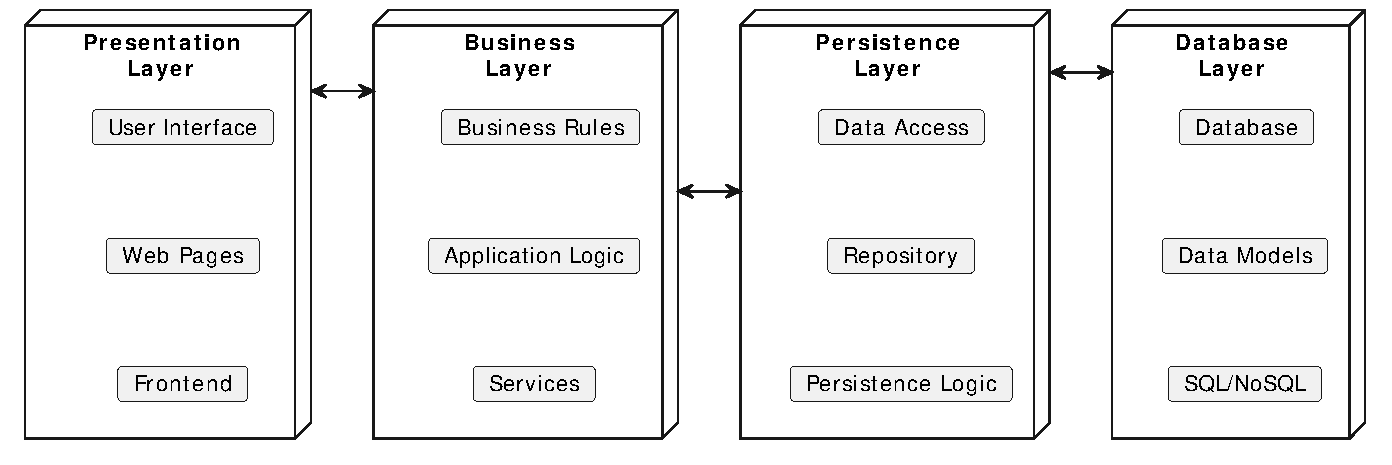
\includegraphics[width=\textwidth]{images/out/layered_architecture.pdf}
	\caption{Layered Architecture Diagram}
	\label{fig:layered_architecture}
\end{figure}

The architecture presented here follows a layered structure, often referred to as a \textbf{four-layered architecture}, which helps in organizing and structuring software applications in a way that separates concerns and improves maintainability, scalability, and flexibility. In this section, we will discuss the layers in detail, examining their roles and responsibilities, as well as how they interact with one another. One instance of layered architecture is a topology that consists of presentation, business, persistence, and database layers. Of course, there are other instances of layered architecture, such as Containerized Architecture (App Layer, Docker Layer, Host OS Layer, Infrastructure Layer), OSI Model (Application Layer, Presentation Layer, Session Layer, Microkernel Architecture (Core Layer, Extension Layer), etc.

\subsection{Presentation Layer}

The \textbf{Presentation Layer} is the topmost layer of the architecture, designed to manage the interaction between the user and the system. It is responsible for presenting information to the user and receiving input from the user. In the context of web applications, this layer typically includes elements like web pages, user interfaces, and the frontend logic. Components in this layer handle user requests and present the data in a user-friendly format.

In the diagram, this layer consists of the following components:
\begin{itemize}
	\item \textbf{User Interface (UI)}: The part of the application that the user interacts with directly, including buttons, forms, and other interface elements.
	\item \textbf{Web Pages}: The various pages that make up the application’s frontend, such as home pages, dashboards, and form submissions.
	\item \textbf{Frontend}: The overall frontend architecture, which might include JavaScript, CSS, and HTML, as well as frameworks like React or Angular.
\end{itemize}

The Presentation Layer communicates with the next layer, the Business Layer, to fetch or send data based on user interactions.

\subsection{Business Layer}

The \textbf{Business Layer}, also known as the \textit{Application Logic} or \textit{Domain Logic} layer, is where the core functionality of the application resides. This layer is responsible for implementing business rules and logic that define how the application should behave. It encapsulates the decisions, processes, and actions that drive the application’s functionality. 

In the diagram, this layer includes, but not limited to, the following components:
\begin{itemize}
	\item \textbf{Business Rules}: These define the core principles and rules of the system, such as how calculations are performed or how data is validated.
	\item \textbf{Application Logic}: This refers to the detailed rules and processes that make up the application’s operation, including handling user input and managing state transitions.
	\item \textbf{Services}: Services may include external services or internal service layers that perform specific tasks, such as sending emails, processing payments, or managing sessions.
\end{itemize}

The Business Layer acts as a mediator between the Presentation and Persistence layers. It is in this layer where business logic is applied, and it decides which data to retrieve or modify from the Persistence Layer based on user actions in the Presentation Layer.

\subsection{Persistence Layer}

The \textbf{Persistence Layer} is responsible for managing the data access and storage of the application. It defines how data is stored, retrieved, and updated, typically using databases or other forms of storage. This layer ensures that the business logic can interact with data without directly dealing with low-level storage operations.

In the diagram, the Persistence Layer consists of, but not limited to, the following components:
\begin{itemize}
	\item \textbf{Data Access}: This component handles the interaction with data storage systems, providing the necessary queries or commands to interact with the database.
	\item \textbf{Repository}: A repository serves as a collection of objects that abstract the retrieval, update, and deletion of data entities.
	\item \textbf{Persistence Logic}: The logic that governs how data is stored, ensuring that the data is in a consistent and retrievable state.
\end{itemize}

This layer communicates with the Database Layer, ensuring that data is accurately and efficiently stored and retrieved when needed by the Business Layer.

\subsection{Database Layer}

The \textbf{Database Layer} is the foundational layer where data is stored persistently. It includes the database itself and the data models that represent the structure of the data. This layer is responsible for ensuring the integrity, consistency, and security of the data.

In the diagram, this layer consists of, but not limited to, the following components:
\begin{itemize}
	\item \textbf{Database}: The actual database system used to store application data, such as MySQL, PostgreSQL, or NoSQL databases like MongoDB.
	\item \textbf{Data Models}: The data models define the structure of the data stored in the database, such as tables in relational databases or collections in NoSQL systems.
	\item \textbf{SQL/NoSQL}: Refers to the types of databases used, whether structured query language (SQL) databases like MySQL or non-relational (NoSQL) databases like MongoDB, each having its own specific use cases.
\end{itemize}

The Database Layer provides data persistence and integrity, ensuring that data remains available even after the application has been shut down or restarted.

\subsection{Layer Interactions}

Each of these layers communicates with adjacent layers to fulfill the application’s requirements. The flow of data can be described as follows:

\begin{itemize}
	\item The \textbf{Presentation Layer} sends user input to the \textbf{Business Layer}, requesting operations or data retrieval.
	\item The \textbf{Business Layer} processes the request, applying business logic, and then communicates with the \textbf{Persistence Layer} to retrieve or modify data.
	\item The \textbf{Persistence Layer} accesses the database, performing the necessary operations to satisfy the request from the Business Layer.
	\item The \textbf{Database Layer} provides the data to the Persistence Layer, which then sends it back to the Business Layer, and eventually the Presentation Layer, where it is presented to the user.
\end{itemize}

By using a layered architecture, the system maintains a high degree of separation of concerns, ensuring that each layer is responsible for a specific aspect of the application’s operation. This separation makes it easier to modify, extend, or replace individual components without affecting the rest of the system.

\section{Closed and Open Layer Architectures}

In software design, layered architecture plays a pivotal role in organizing the system's components. A common pattern involves the use of closed and open layers, which determine the degree of interaction and accessibility between various system components. The diagram below illustrates the concepts of closed and open layers in a system architecture.

\begin{figure}[ht]
	\centering
	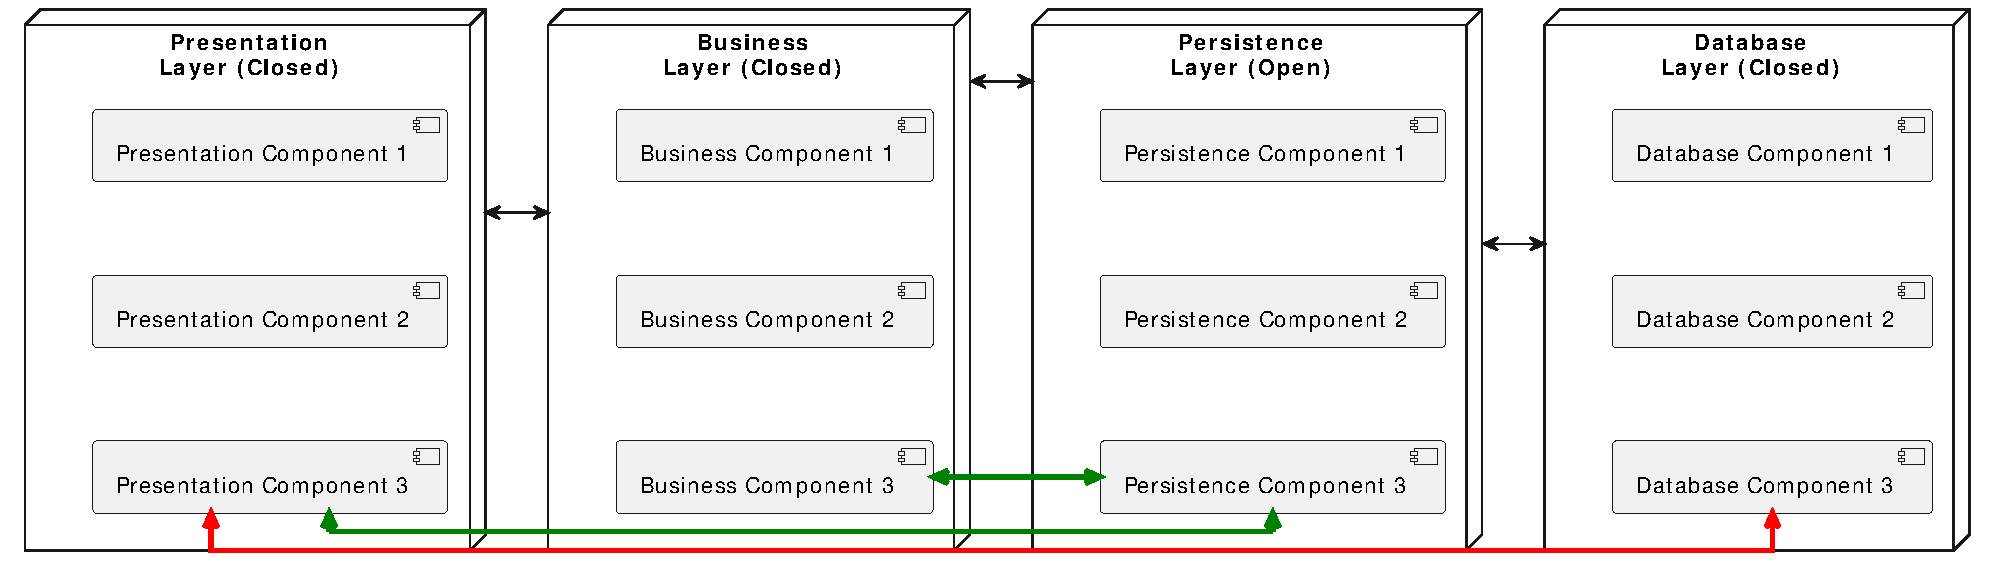
\includegraphics[width=\textwidth]{images/out/layered_architecture_open.pdf}
	\caption{Closed and Open Layer Architectures}
	\label{fig:layered_architecture_open}
\end{figure}

\subsection{Closed Layer Architecture}

A closed layer architecture refers to layers where components within the layer can only interact with other components within the same layer or with adjacent layers. This restricts direct external access to the components of the layer. The closed nature of these layers provides security, stability, and encapsulation of logic. 

In the diagram, both the \textbf{Presentation Layer} and the \textbf{Database Layer} are considered closed layers. The components within these layers are isolated from external interactions. Specifically:
\begin{enumerate}
	\item The \textbf{Presentation Layer} consists of components such as \textit{Presentation Component 1}, \textit{Presentation Component 2}, and \textit{Presentation Component 3}. These components interact only with adjacent layers and not with external entities directly.
	\item The \textbf{Database Layer} comprises components like \textit{Database Component 1}, \textit{Database Component 2}, and \textit{Database Component 3}. These components are shielded from direct external modifications.
\end{enumerate}

It is important to note that the red connection between \textit{Presentation Component 3} and \textit{Database Component 3} is prohibited because the \textbf{Database Layer} is closed. In a closed layer architecture, components within the layer should not have direct access to or interact with external layers outside of the adjacent layer. Therefore, any communication between the \textbf{Presentation Layer} and the \textbf{Database Layer} must occur through the \textbf{Persistence Layer}, which acts as the intermediary.

This prohibition ensures that the closed nature of the layers is maintained, enforcing proper encapsulation, and keeping the system's components well-separated. The access from \textit{Presentation Component 3} to \textit{Database Component 3} would break this rule and is therefore not allowed in this architecture.

Examples where a closed layer architecture is preferred include:
\begin{enumerate}
	\item \textbf{Banking Systems:} In banking applications, the \textbf{Presentation Layer} (e.g., web interfaces, mobile apps) and the \textbf{Database Layer} (e.g., user data, transaction records) must remain isolated to ensure sensitive data is not exposed. This design prevents any direct interaction between the user interface and the database, mitigating the risk of data breaches.
	\item \textbf{Healthcare Systems:} In healthcare applications, patient data and treatment records stored in the \textbf{Database Layer} should not be directly accessible by the \textbf{Presentation Layer}. Instead, any access to the database should go through the \textbf{Persistence Layer} to ensure data validation, security, and privacy regulations are enforced.
\end{enumerate}

\subsection{Open Layer Architecture}

An open layer allows greater flexibility and external interaction. Open layers expose their components to communication from other layers, making them more adaptable for various integrations. The open nature of these layers enables data exchange and functionality access across layers.

In the provided diagram, the \textbf{Persistence Layer} is an open layer. The components \textit{Persistence Component 1}, \textit{Persistence Component 2}, and \textit{Persistence Component 3} allow external interactions, particularly with other layers.

In the diagram, \textit{Persistence Component 3} interacts directly with both \textit{Presentation Component 3} and \textit{Business Component 3}, as shown by the green connections. This direct interaction exemplifies an open layer design that prioritizes flexibility and performance over encapsulation.

Two examples of when an open layer architecture is appropriate include:

\begin{enumerate}
	\item \textbf{Performance Considerations:} In a performance-sensitive application where reducing latency is critical (e.g., real-time systems), it may be beneficial for the \textbf{Presentation Layer} or \textbf{Business Layer} to access the \textbf{Persistence Layer} directly. Bypassing intermediary layers reduces the overhead introduced by additional communication steps, thus improving performance.
	\item \textbf{Lack of Security Concerns:} If the application operates in a controlled environment with less stringent security requirements (e.g., an internal tool or a non-sensitive system), direct communication with the \textbf{Persistence Layer} can be acceptable. In such scenarios, there may be less concern about exposing certain components to external access, as the risk is deemed minimal.
\end{enumerate}


\section{Advantages and Disadvantages of Layered Architecture}

Layered architecture is a popular software design pattern that separates a system into distinct layers, each responsible for a specific functionality. This separation allows for modular development, better organization, and maintenance. However, like any design pattern, layered architecture comes with its own set of advantages and disadvantages. In this section, we explore both sides of using a layered approach in system design.

\subsection{Advantages of Layered Architecture}

\begin{enumerate}
	\item \textbf{Separation of Concerns:} 
	One of the primary benefits of layered architecture is the clear separation of concerns between different parts of the system. Each layer is responsible for a specific aspect of the system, such as presentation, business logic, or data persistence. This separation improves readability, reduces complexity, and helps developers focus on one layer at a time without worrying about other concerns.
	
	\item \textbf{Modularity and Maintainability:} 
	Layered architecture encourages modular design by isolating components into distinct layers. This modularity makes it easier to maintain, as changes in one layer (e.g., database modifications or changes to business rules) can often be made without affecting other layers. Additionally, individual layers can be updated or replaced independently, promoting code reuse and simplifying maintenance.
	
	\item \textbf{Scalability:} 
	Layered systems often provide better scalability due to their separation of concerns. Different layers can be scaled independently based on their load. For example, if the presentation layer experiences high traffic, additional servers can be added to handle the load, without impacting the underlying business or persistence layers.
	
	\item \textbf{Testability:} 
	With clear separation between layers, individual components can be easily isolated and tested. Unit tests can focus on specific layers (e.g., testing business logic without needing to interact with the database), which improves test coverage and reduces the chances of bugs.
	
	\item \textbf{Flexibility in Technology Choices:} 
	Layered architecture allows different layers to use different technologies and frameworks. For example, the presentation layer could use a web framework like React, while the business layer could use a Java-based service, and the persistence layer could be built with a NoSQL database. This flexibility in technology choice can help developers use the best tool for each layer's purpose.
\end{enumerate}

\subsection{Disadvantages of Layered Architecture}

\begin{enumerate}
	\item \textbf{Performance Overhead:} 
	One of the main drawbacks of layered architecture is the potential performance overhead introduced by the multiple layers. Each layer adds a level of abstraction and can introduce additional processing time due to the need for inter-layer communication. In high-performance applications, this can lead to latency issues, especially when layers communicate over networked environments.
	
	\item \textbf{Complexity in Simple Systems:} 
	For smaller applications with limited functionality, a layered architecture may introduce unnecessary complexity. In such cases, the overhead of maintaining multiple layers may not provide significant benefits. A simpler monolithic or component-based architecture might be more suitable for these systems.
	
	\item \textbf{Tight Coupling Between Layers:} 
	While layered architecture promotes separation of concerns, it can also lead to tight coupling between layers. If one layer depends heavily on the implementation details of another, changes in one layer may require corresponding changes in others. This can make the system harder to refactor and may reduce flexibility over time.
	
	\item \textbf{Rigidity in Layering:} 
	Layered architecture can become rigid as it enforces strict separation between layers. In some cases, it may not be possible to bypass a layer or modify its interaction with others without significant refactoring. This rigidity can limit the system's adaptability to changing requirements.
	
	\item \textbf{Difficulty in Managing Cross-Cutting Concerns:} 
	Certain concerns, such as security, logging, and transaction management, often span multiple layers. In a layered architecture, managing these cross-cutting concerns can be difficult and lead to redundant code. These concerns often require special handling, such as using aspect-oriented programming (AOP) or middleware.
\end{enumerate}

\subsection{Advantages and Disadvantages of Closed Layer Architecture}

\subsubsection{Advantages of Closed Layer Architecture}

\begin{enumerate}
	\item \textbf{Security and Encapsulation}: By isolating layers, components within a closed layer are protected from external access, ensuring that sensitive data or logic remains hidden from unauthorized components or users.
	\item \textbf{Stability}: Restricting communication to adjacent layers reduces the risk of unintended interactions and minimizes errors or unexpected behaviors that could arise from external access.
	\item \textbf{Maintainability}: With encapsulated components and limited access, it becomes easier to make changes to internal logic without impacting other parts of the system.
\end{enumerate}

\subsubsection{Disadvantages of Closed Layer Architecture}

\begin{enumerate}
	\item \textbf{Limited Flexibility}: Restricting communication to adjacent layers can limit flexibility and may create complexities when needing to introduce new layers or require more direct interaction between layers.
	\item \textbf{Increased Complexity in Communication}: Because external components cannot directly communicate with closed layers, the design must rely on adjacent layers as intermediaries, which can lead to more complex interactions.
	\item \textbf{Potential Performance Overhead}: Introducing additional intermediary layers (e.g., Persistence Layer) for communication can lead to performance bottlenecks if not designed efficiently.
\end{enumerate}

\subsection{Advantages and Disadvantages of Open Layer Architecture}

\subsubsection{Advantages of Open Layer Architecture}

\begin{enumerate}
	\item \textbf{Increased Flexibility}: Open layers allow direct communication between components across different layers, making it easier to introduce new components or integrate with external systems without excessive intermediaries.
	\item \textbf{Improved Performance}: Since there is no need for intermediaries, open layers can improve performance by reducing the overhead of additional communication steps between layers.
	\item \textbf{Simplified Communication}: Open layers make it easier to design systems where multiple components need to interact or exchange data directly, without relying on intermediary layers.
\end{enumerate}

\subsubsection{Disadvantages of Open Layer Architecture}

\begin{enumerate}
	\item \textbf{Security Risks}: Direct access to open layers can expose the system to potential security vulnerabilities, as unauthorized components or users may gain access to critical data or business logic.
	\item \textbf{Reduced Encapsulation}: Open layers expose internal components, which may compromise encapsulation and make it harder to protect the integrity of the system’s design.
	\item \textbf{Maintenance Challenges}: With increased external interactions, maintaining the integrity of the system can become more challenging, as changes to one layer can potentially affect others.
\end{enumerate}




%%\gny{Tolong tambahkan keterangan gambar contoh : Gambar 5.1, 5.2, dst.. dan tambahkan italic text untuk setiap bahasa asing}
%
%
%\section{Definisi \textit{Layered Architechture}}
%
%Pola arsitektur \textit{layered} adalah pola \textit{n-tiered} di mana komponen disusun dalam lapisan horizontal. Ini adalah metode tradisional untuk merancang sebagian besar perangkat lunak dan dimaksudkan untuk pengembangan mandiri sehingga semua komponen saling berhubungan tetapi tidak saling bergantung.
%
%\includegraphics[width=\textwidth]{../images/Layering Architecture}
%\begin{center}
%	Gambar 5.1 \textit{Layering Architecture}
%\end{center}
%
%Seperti yang ditunjukkan pada gambar, \textit{layering} biasanya dilakukan dengan mengemas fungsionalitas khusus aplikasi di lapisan atas, penyebaran fungsionalitas spesifik menjadi lapisan bawah dan fungsionalitas yang membentang di seluruh domain aplikasi di lapisan tengah. Jumlah lapisan dan bagaimana lapisan-lapisan ini disusun ditentukan oleh kompleksitas masalah dan solusinya.
%
%Di sebagian besar arsitektur berlapis, ada beberapa lapisan (atas ke bawah):
%
%\begin{itemize}
%    \item \textbf{\textit{The application layered}:} Berisi layanan spesifik aplikasi.
%    \item \textbf{The business layer:} Menangkap komponen yang umum di beberapa aplikasi.
%    \item \textbf{\textit{The middleware layer}:} Lapisan ini mengemas beberapa fungsi seperti pembangun GUI, antarmuka ke basis data, laporan, dan dll.
%    \item \textbf{\textit{The database/System Software Layer}:} Berisi OS, \textit{database}, dan antarmuka ke komponen perangkat keras tertentu.
%\end{itemize}
%
%\section{Latar Belakang}
%
%Penilaian untuk setiap karakteristik berdasarkan kecenderungan alami untuk implementasi tipikal pola \textit{layered}.
%
%\begin{itemize}
%    \item Kemampuan untuk merespon dengan cepat terhadap lingkungan yang terus berubah. (monolitik)
%    \item Bergantung pada implementasi pola, penyebaran bisa menjadi masalah. Satu perubahan kecil ke komponen dapat memerlukan \textit{redeployment} seluruh aplikasi.
%    \item Pengembang dapat memberikan pengujian singkat untuk menguji aplikasi sebelum klien menggunakannya
%    \item Mudah dikembangkan karena polanya sudah terkenal dan tidak terlalu rumit untuk melakukan implementasinya.
%\end{itemize}
%
%\section{Pros Cons}
%
%\subsection{Pros}
%
%\begin{itemize}
%    \item Mudah untuk diuji karena komponen-komponennya termasuk lapisan khusus sehingga dapat diuji secara terpisah.
%    \item Sederhana dan mudah diimplementasikan karena secara alami, sebagian besar aplikasi bekerja berlapis-lapis
%\end{itemize}
%
%\subsection{Cons}
%
%\begin{itemize}
%    \item Tidak mudah untuk melakukan perubahan pada lapisan tertentu karena aplikasi merupakan unit tunggal.
%    \item Kopling antar lapisan cenderung membuatnya lebih sulit. Hal ini membuatnya sulit untuk diukur.
%    \item Harus digunakan sebagai unit tunggal sehingga perubahan ke lapisan tertentu berarti seluruh sistem harus dipekerjakan kembali.
%    \item Semakin besar, semakin banyak sumber daya yang dibutuhkan untuk permintaan untuk melewati beberapa lapisan dan dengan demikian akan menyebabkan masalah kinerja.
%\end{itemize}
%
%\section{Software Architechture Pattern}
%Ini adalah pola arsitektur paling umum di sebagian besar aplikasi tingkat perusahaan. Ini juga dikenal sebagai pola n-tier, dengan asumsi n jumlah tingkatan. Contoh Skenario:
%
%\includegraphics[width=\textwidth]{../images/Software Architecture Pattern}
%\begin{center}
%	Gambar 5.2 \textit{Software Architecture Pattern}
%\end{center}
%
%
%\section{Design Patterns}
%
%Anggap \textit{mock-up software design}, susunan “\textit{stack}” nya seperti \textit{layered architecture}:
%
%\includegraphics[width=\textwidth]{../images/Design Pattern}
%\begin{center}
%	Gambar 5.3 \textit{Design Pattern}
%\end{center}
%
%Setiap \textit{layer} dari aplikasi terpisah dengan cara penggunaan metode API, namun yang masih saling berhubungan adalah \textit{memory handling} , karena setiap komunikasi \textit{layer} akan membawa/mengirim data sehingga akan terjadi alokasi \textit{memory} dan pada akhirnya membutuhkan \textit{memory handling}.
%
%Ada 4 bagian dari \textit{layered architecture} yang di mana setiap layer memiliki hubungan antara komponen yang ada di dalamnya dari atas ke bawah yaitu:
%
%\begin{itemize}
%    \item \textbf{\textit{The presentation layer}:} Semua bagian yang berhubungan dengan layer presentasi.
%    \item \textbf{\textit{The business layer}:} Berhubungan dengan logika bisnis.
%    \item \textbf{\textit{The persistence layer}:} Berguna untuk mengurusi semua fungsi yang berhubungan dengan objek relasional
%    \item \textbf{\textit{The database layer}:} Tempat penyimpanan semua data layer.
%\end{itemize}
%
%\subsection{Contoh penerapan \textit{layered architecture}:}
%
%\includegraphics[width=\textwidth]{../images/contoh}
%\begin{center}
%	Gambar 5.4 Contoh penerapan \textit{layered architecture}
%\end{center}
%

%\chapter{Model-View-* Architectures}

\section{Pendahuluan}

Model-View-* (MV*) adalah sekumpulan arsitektur yang digunakan dalam pengembangan perangkat lunak untuk memisahkan logika bisnis dari antarmuka pengguna. Pendekatan ini bertujuan untuk meningkatkan pemisahan tanggung jawab, mempermudah pengujian, serta meningkatkan keterbacaan dan pemeliharaan kode. Berbagai varian MV* meliputi \textit{Model-View-Controller} (MVC), \textit{Model-View-Presenter} (MVP), \textit{Model-View-ViewModel} (MVVM), dan \textit{Model-View-Intent} (MVI), masing-masing dengan karakteristik dan implementasi yang berbeda dalam berbagai lingkungan pengembangan.

MVC adalah pola desain yang awalnya diperkenalkan untuk mengorganisasi kode aplikasi dengan membagi tanggung jawab menjadi tiga komponen utama: \textit{Model}, yang mewakili data dan logika bisnis, \textit{View}, yang mengelola antarmuka pengguna, dan \textit{Controller}, yang bertindak sebagai mediator antara Model dan View. Seiring berkembangnya teknologi, muncul variasi MV* lainnya, seperti MVP, yang menekankan pemisahan logika presentasi dan View melalui \textit{Presenter}, MVVM, yang diperkenalkan dalam pengembangan berbasis binding data, dan MVI, yang banyak digunakan dalam pengembangan aplikasi reaktif.

Bab ini memberikan pembahasan mendalam mengenai setiap arsitektur Model-View-*, termasuk konsep dasar, perbedaan utama, keuntungan dan kerugian, serta implementasinya dalam berbagai teknologi. Contoh dunia nyata juga disajikan untuk menggambarkan bagaimana pola-pola ini diterapkan dalam pengembangan perangkat lunak modern.

\section{Model-View-Controller (MVC)}

Model-View-Controller (MVC) merupakan pola desain perangkat lunak yang memisahkan aplikasi menjadi tiga bagian utama untuk meningkatkan modularitas dan kemudahan pemeliharaan.

\subsection{MVC Klasik}

Pada implementasi klasik, MVC membagi aplikasi menjadi tiga komponen:

\begin{itemize}
	\item \textbf{Model} menangani data, logika bisnis, dan aturan bisnis aplikasi.
	\item \textbf{View} bertanggung jawab atas representasi data kepada pengguna.
	\item \textbf{Controller} menghubungkan Model dan View, menangani input pengguna, dan memperbarui Model serta View sesuai kebutuhan.
\end{itemize}

Diagram berikut menggambarkan arsitektur MVC klasik:

\begin{figure}[h]
	\centering
	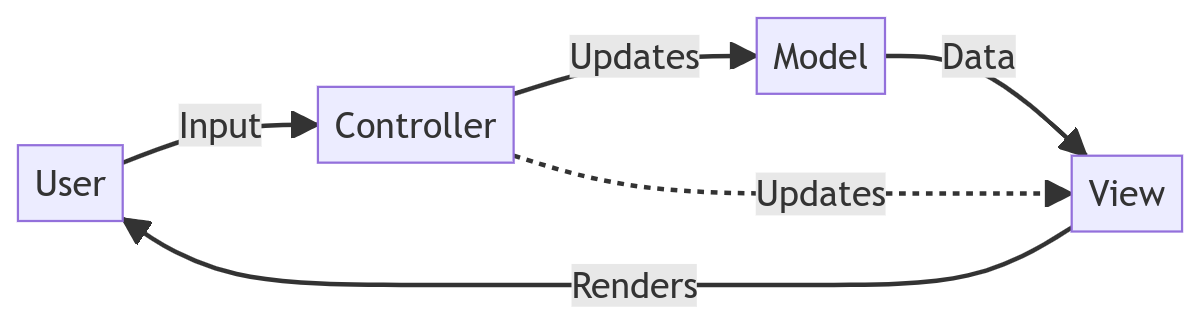
\includegraphics[width=\textwidth]{../images/mvc-classic.png}
	\caption{Classic MVC model when Users with controllers not screens}
	\label{fig:mvc-classic}
\end{figure}

\subsection{MVC dalam Kerangka Web dan Aplikasi Desktop Modern}

Banyak kerangka kerja web modern, seperti Laravel, Django, dan Spring, serta aplikasi desktop seperti JavaFX, menggunakan pendekatan MVC yang sedikit berbeda. Dalam implementasi ini:

\begin{itemize}
	\item Controller sering kali memiliki peran lebih besar, menangani logika bisnis dan interaksi dengan Model.
	\item View tidak hanya menampilkan data tetapi juga dapat berisi kode pemrograman untuk rendering dinamis.
	\item Model sering kali terintegrasi dengan ORM (\textit{Object-Relational Mapping}) untuk mempermudah akses ke basis data.
\end{itemize}

Diagram berikut menggambarkan perbedaan antara MVC klasik dan yang digunakan dalam kerangka kerja web dan aplikasi desktop modern:

\begin{figure}[h]
	\centering
	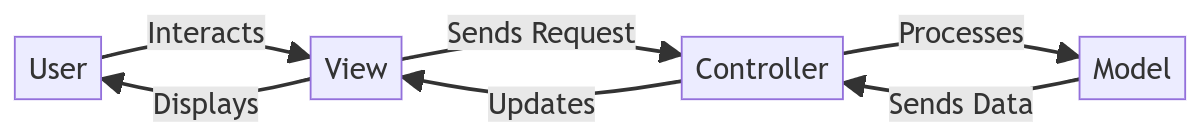
\includegraphics[width=\textwidth]{../images/mvc-modern.png}
	\caption{MVC in modern desktop/web frameworks.}
	\label{fig:mvc-modern}
\end{figure}

Pendekatan dalam kerangka kerja modern memungkinkan pemisahan lebih baik antara logika bisnis dan antarmuka pengguna, sekaligus mengintegrasikan teknologi seperti API REST dan AJAX untuk interaksi yang lebih dinamis.


\section{Model-View-Presenter (MVP)}

Model-View-Presenter (MVP) adalah pola desain yang mirip dengan MVC namun memiliki perbedaan signifikan dalam cara interaksi antara komponen-komponen tersebut. MVP lebih banyak digunakan dalam aplikasi desktop atau aplikasi yang membutuhkan pengendalian lebih besar terhadap tampilan dan interaksi pengguna. Dalam implementasi MVP:

\begin{itemize}
	\item \textbf{Model} bertanggung jawab untuk menangani logika bisnis dan data. Ini berinteraksi dengan basis data dan menyediakan data yang diperlukan oleh Presenter.
	\item \textbf{View} hanya bertugas untuk menampilkan antarmuka pengguna dan tidak mengandung logika bisnis. View akan menerima input dari pengguna dan meneruskannya ke Presenter. View bersifat pasif, artinya tidak mengelola pengolahan data atau logika bisnis.
	\item \textbf{Presenter} bertindak sebagai penghubung antara Model dan View. Presenter menerima input dari View, memprosesnya (dengan berinteraksi dengan Model), dan kemudian memperbarui View dengan data yang diperlukan.
\end{itemize}

Perbedaan utama antara \textbf{MVP} dan \textbf{MVC Klasik} terletak pada bagaimana komponen-komponen tersebut berinteraksi:
\begin{itemize}
	\item Dalam \textbf{MVP}, \textbf{Presenter} memiliki peran yang lebih besar. Semua logika bisnis dan pengolahan data dikelola oleh Presenter. View bertanggung jawab hanya untuk menampilkan data dan menerima input dari pengguna, tetapi tidak menangani pengolahan atau logika bisnis. Presenter mengelola interaksi antara Model dan View.
	\item Dalam \textbf{MVC Klasik}, \textbf{Controller} bertanggung jawab untuk menangani logika bisnis dan interaksi antara Model dan View. View hanya menampilkan data dan berinteraksi langsung dengan Controller. Dengan kata lain, Controller mempengaruhi tampilan berdasarkan aksi pengguna dengan mengubah Model, sedangkan View hanya berfungsi untuk menampilkan antarmuka pengguna.
	\item Dalam \textbf{MVP}, komunikasi antara View dan Presenter adalah dua arah, sementara dalam \textbf{MVC Klasik}, komunikasi lebih cenderung satu arah dari Controller ke View atau Model ke View.
\end{itemize}

Diagram berikut menggambarkan arsitektur MVP dan perbedaan utamanya dengan MVC Klasik:

\begin{figure}[h]
	\centering
	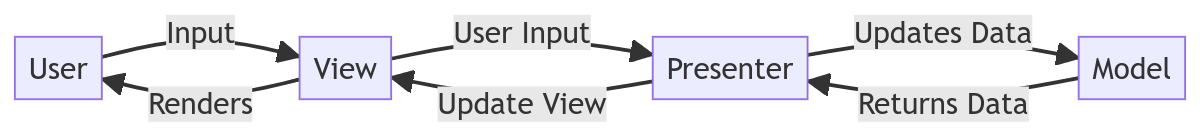
\includegraphics[width=\textwidth]{../images/mvp.png}
	\caption{Model-View-Presenter Architecture.}
	\label{fig:mvp-architecture}
\end{figure}

Keuntungan utama dari MVP adalah pemisahan yang jelas antara logika bisnis dan antarmuka pengguna, serta kemudahan pengujian unit karena Presenter dapat diuji secara terpisah tanpa bergantung pada View.

\section{Model-View-ViewModel (MVVM)}

Model-View-ViewModel (MVVM) adalah pola desain yang lebih banyak digunakan dalam aplikasi desktop dan aplikasi berbasis WPF (Windows Presentation Foundation) atau platform lain yang mendukung binding data dua arah. MVVM memisahkan logika presentasi dari antarmuka pengguna dengan cara yang sangat terstruktur. Dalam implementasi MVVM:

\begin{itemize}
	\item \textbf{Model} bertanggung jawab untuk menangani logika bisnis dan data. Model ini berinteraksi dengan basis data atau layanan lain untuk menyediakan data yang diperlukan oleh ViewModel.
	\item \textbf{View} bertanggung jawab untuk menampilkan antarmuka pengguna dan menerima input dari pengguna. View hanya berfokus pada rendering dan tidak mengelola logika atau data.
	\item \textbf{ViewModel} adalah penghubung antara View dan Model. ViewModel menangani logika presentasi, memanipulasi data yang diterima dari Model, dan menyediakan data tersebut dalam bentuk yang dapat digunakan oleh View. Dalam MVVM, ViewModel berinteraksi dengan View menggunakan binding data dua arah, yang memungkinkan pembaruan secara otomatis antara View dan ViewModel.
\end{itemize}

Perbedaan utama antara \textbf{MVVM} dan \textbf{MVP} terletak pada peran **ViewModel** dalam MVVM:
\begin{itemize}
	\item Dalam \textbf{MVVM}, \textbf{ViewModel} berfungsi untuk mempersiapkan data dari Model agar dapat digunakan oleh View. ViewModel mengelola logika presentasi dan menyediakan data dalam format yang dapat langsung dipakai oleh View.
	\item Dalam \textbf{MVP}, \textbf{Presenter} bertanggung jawab untuk memproses input dari View dan mengatur interaksi dengan Model, sementara View hanya menampilkan data dan tidak terlibat dalam pengolahan data atau logika.
	\item Dalam \textbf{MVVM}, komunikasi antara View dan ViewModel menggunakan binding data dua arah, memungkinkan pembaruan otomatis antara keduanya. Sebaliknya, dalam \textbf{MVP}, komunikasi antara View dan Presenter adalah satu arah, dimana Presenter memperbarui View dengan data yang diproses.
\end{itemize}

Diagram berikut menggambarkan arsitektur MVVM dan perbedaan utamanya dengan MVP:

\begin{figure}[h]
	\centering
	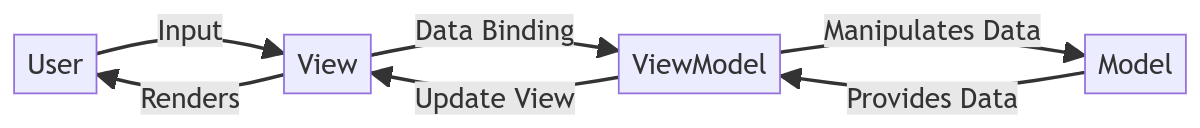
\includegraphics[width=\textwidth]{../images/mvvm.png}
	\caption{Model-View-ViewModel Architecture.}
	\label{fig:mvvm-architecture}
\end{figure}

Keuntungan utama dari MVVM adalah kemampuan untuk memisahkan logika presentasi dari antarmuka pengguna dengan menggunakan binding data dua arah, sehingga membuat pengujian dan pemeliharaan aplikasi lebih mudah. Selain itu, karena ViewModel menangani logika presentasi, View menjadi lebih sederhana dan lebih fokus pada rendering.


\section{Model-View-Intent (MVI)}

Model-View-Intent (MVI) adalah pola desain yang sering digunakan dalam aplikasi modern, terutama dalam pengembangan aplikasi Android. MVI bertujuan untuk menyederhanakan alur data dengan memberikan pendekatan yang lebih deklaratif dan reaktif. Dalam MVI, setiap komponen memiliki peran yang jelas dalam memanipulasi dan mengelola data aplikasi.

Dalam implementasi MVI:

\begin{itemize}
	\item \textbf{Model} berfungsi untuk menangani logika bisnis dan data aplikasi. Model ini menyediakan status atau keadaan aplikasi yang dapat digunakan oleh View. Model mengelola dan menyimpan data yang digunakan oleh aplikasi.
	\item \textbf{View} bertanggung jawab untuk menampilkan antarmuka pengguna dan menerima input dari pengguna. View akan mengirimkan intent ke Presenter atau ViewModel yang akan diproses lebih lanjut. View bersifat reaktif, menerima pembaruan dari Model melalui observasi data.
	\item \textbf{Intent} adalah tindakan atau niat yang dilakukan oleh pengguna yang kemudian diteruskan ke Presenter atau ViewModel untuk diproses. Intent menggambarkan apa yang ingin dilakukan oleh pengguna (misalnya, tombol ditekan atau elemen lainnya dipilih). Intent digunakan untuk memicu perubahan status pada Model atau memulai proses lain yang relevan.
\end{itemize}

Perbedaan utama antara \textbf{MVI} dan \textbf{MVP} terletak pada cara interaksi dan komunikasi antar komponen:
\begin{itemize}
	\item Dalam \textbf{MVI}, \textbf{Intent} menggantikan peran input pengguna yang secara langsung diteruskan ke ViewModel atau Presenter. Intent memfokuskan pada pengelolaan status aplikasi secara reaktif.
	\item Dalam \textbf{MVP}, \textbf{Presenter} bertanggung jawab untuk menangani logika presentasi dan memproses input dari View untuk memperbarui Model.
	\item Dalam \textbf{MVI}, komunikasi adalah satu arah dari Intent ke ViewModel atau Presenter, yang kemudian memodifikasi status Model dan mengirimkan pembaruan kembali ke View.
\end{itemize}

Diagram berikut menggambarkan arsitektur MVI dan perbedaannya dengan pola desain lain seperti MVP:

\begin{figure}[h]
	\centering
	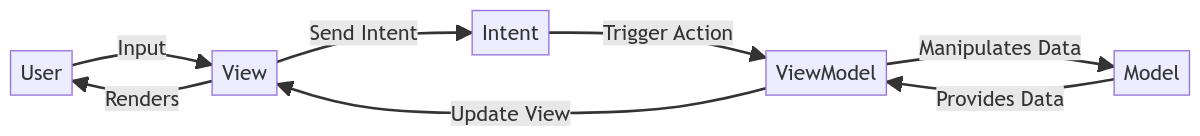
\includegraphics[width=\textwidth]{../images/mvi.png}
	\caption{Model-View-Intent Architecture.}
	\label{fig:mvi-architecture}
\end{figure}

Keuntungan utama dari MVI adalah pengelolaan status aplikasi yang lebih sederhana dan kemampuan untuk menangani alur data yang lebih reaktif. MVI juga memudahkan pemeliharaan kode dengan mengurangi kebingungan terkait interaksi antara View dan Model, serta memperkenalkan pendekatan yang lebih terstruktur untuk menangani state.


%\begin{table}[h]
%	\centering
%	\scriptsize
%	\begin{tabular}{|p{0.08\textwidth}|p{0.19\textwidth}|p{0.19\textwidth}|p{0.19\textwidth}|p{0.19\textwidth}|}
%		\hline
%		\textbf{Fitur} & \textbf{View} & \textbf{Con\-trol\-ler/\-Pre\-sent\-er/\-View\-Mo\-del} & \textbf{Model} & \textbf{Fitur Utama} \\
%		\hline
%		\textbf{MVC (Klasik)} & Menampilkan data, mengirimkan input pengguna ke Controller. & Menangani input pengguna, memperbarui View dan Model. & Menyimpan logika bisnis dan data, berinteraksi dengan basis data. & Pola klasik dengan interaksi langsung antara View, Controller, dan Model. \\
%		\hline
%		\textbf{MVC Modern} & Menampilkan data, mengirimkan input pengguna ke Controller, mungkin juga termasuk kode rendering dinamis. & Menangani input pengguna, mungkin termasuk logika tambahan, memperbarui View dan Model. & Menyimpan logika bisnis dan data, mungkin menggunakan ORM untuk pengelolaan data. & Interaksi lebih dinamis dengan logika tambahan di Controller, termasuk AJAX atau API REST. \\
%		\hline
%		\textbf{MVP} & Menampilkan data, mengirimkan input pengguna ke Presenter. & Menangani input pengguna, berinteraksi dengan Model, memperbarui View. & Menyimpan logika bisnis dan data, berinteraksi dengan basis data. & Presenter menangani seluruh logika dan pemrosesan data, \textbf{View bersifat pasif}. \\
%		\hline
%		\textbf{MVVM} & Menampilkan data, mengikat ke ViewModel menggunakan \textbf{binding data} dua arah. & Menangani logika presentasi, memanipulasi data dari Model, memperbarui View. & Menyimpan logika bisnis dan data, berinteraksi dengan basis data. & ViewModel mengikat data secara reaktif dengan View, mendukung binding data dua arah. \\
%		\hline
%		\textbf{MVI} & Menampilkan data, mengirimkan input pengguna sebagai \textbf{Intent} ke ViewModel. & Menangani pemrosesan logika, memanipulasi data dari Model, memperbarui View secara reaktif. & Menyimpan logika bisnis dan data, menyediakan pembaruan data ke ViewModel. & Pembaruan reaktif berbasis Intent, pengelolaan status disederhanakan. \\
%		\hline
%	\end{tabular}
%	\caption{Perbandingan Antara MVC (Klasik), MVC Modern, MVP, MVVM, dan MVI}
%	\label{tab:framework-comparison}
%\end{table}



%\section{Latar Belakang}
%Pada mulanya, dalam pengembangan perangkat lunak, kode yang bertanggung jawab terhadap data, logika bisnis, dan tampilan (Graphical User Interface) bercampur jadi satu, tidak ada pemisahan abstraksi.
%Pola Model-View-Controller kemudian muncul memisahkan kode program ke dalam 3 abstraksi utama berdasarkan perhatian mereka: \textit{model} untuk data, \textit{view} untuk tampilan, dan \textit{controller} untuk logika bisnis. 
%Hanya saja, MVC tidak memiliki abstraksi yang secara eksplisit mengelola \textit{states} dari tampilan (\textit{views}).
%Pola MVP (Model-View-Presenter) kemudian diajukan di mana komponen \textit{Presenter}-nya bertanggung jawab mengelola logika presentasi dari \textit{views}. Walaupun demikian,kode program yang mengelola sinkronisasi antara views dan state dari logika presentasi mereka masih harus dibuat secara manual.
%
%Keunikan dari Model-View-ViewModel adalah pola tersebut memiliki komponen \textit{binder} yang mengotomasi komunikasi/sinkronisasi antara view dengan properties yang ada pada \textit{view model}. Nilai-nilai pada \textit{view} ditautkan dengan properties pada view model sehingga perubahan nilai pada salah komponen di view (misalnya perubahan pada \textit{textbox}) akan memperbarui juga nilai pada \textit{property}-nya di \textit{view model} yang ditautkan pada komponen tersebut. Adanya binder mengurangi jumlah kode yang harus ditulis oleh developer secara manual untuk melakukan sinkronisasi antara \textit{view} dan \textit{view model}.
%
%\begin{figure}[h]
%    \centering
%    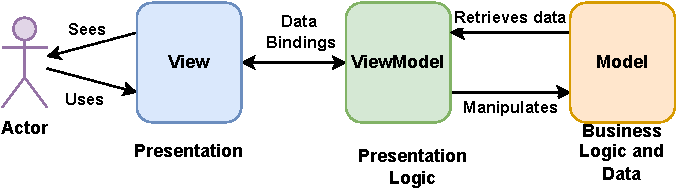
\includegraphics[width=\textwidth]{mvvm}
%    \caption{Arsitektur Model-View-ViewModel (MVVM).}
%    \label{fig:mvvm}
%\end{figure}
%
%
%\section{Arsitektur Model-View-ViewModel}
%\begin{itemize}
%\item Separation of the view layer by moving all GUI code to the view model via data binding.
%\item UI developers don't write the the GUI, instead a markup language is used.
%\item The separation of roles allows UI designers to focus on the UX design rather than programming of the business logic. 
%\item A proper separation of the view from the model is more productive, as the user interface typically changes frequently and late in the development cycle based on end-user feedback.
%\item Data bindings and properties are used to synchronise the relevant values in the view and the view model, that represents the state of the view, so that they are always the same.
%\item It eliminates or minimises application logic that directly manipulates the view. 
%
%\end{itemize}
%
%
%
%\section{Kelebihan dan Kekurangan}
%Berikut adalah kelebihan dan kekurangan arsitektur MVVM:
%
%
%\subsection{Kelebihan}
%Keuntungan dari menerapkan arsitektur MVVM adalah:
%\begin{itemize}
%\item Separation of the view layer by moving all GUI code to the view model via data binding.
%\item UI developers don't write the the GUI, instead a markup language is used.
%\item The separation of roles allows UI designers to focus on the UX design rather than programming of the business logic. 
%\item A proper separation of the view from the model is more productive, as the user interface typically changes frequently and late in the development cycle based on end-user feedback.
%\item Data bindings and properties are used to synchronise the relevant values in the view and the view model, that represents the state of the view, so that they are always the same.
%\item It eliminates or minimises application logic that directly manipulates the view. 
%
%\end{itemize}
%
%\subsection{Kekurangan}
%Konsekuensi dari penerapan arsitektur MVVM adalah sebagai berikut:
%\begin{itemize}
%\item It can be overkill for small projects. 
%\item Generalizing the viewmodel upfront can be difficult for large applications.
%\item Large-scale data binding can lead to lower performance.
%\item It's best for UI development but might not the best for other types of developments and  applications.
%\end{itemize}
%
%\section{Contoh Kasus}
%
%\subsection{Deskripsi}
%Jelaskan contoh kasus yang dipaparkan berkaitan dengan arsitektur yang dimaksud pada bab ini.
%Contoh kasus harus memperjelas arsitektur yang dimaksud.
%
%\subsection{Penjelasan Implementasi}
%Jelaskan bagian-bagian kode program, basisdata, atau konfigurasi yang signifikan terhadap arsitektur yang dimaksud.
%
%\begin{lstlisting}[firstnumber=1,style=java,caption={Model dari \textsf{Rate}.},label=lst:rate_model]
%import javax.persistence.Entity;
%import javax.persistence.Id;
%import javax.persistence.IdClass;
%
%@Entity
%@IdClass(RateId.class)
%public class Rate {
%  @Id
%  private String fromCurrency;
%  @Id
%  private String toCurrency;
%  private Double rate;
%  ...
%  Rate(String fromCurrency, String toCurrency, Double rate) {
%    ...
%  }
%  ...
%}
%\end{lstlisting}
%
%\begin{lstlisting}[firstnumber=1,style=java,caption={ \textsf{RateRepository}.},label=lst:rate_repository]
%import java.util.Collection;
%import org.springframework.data.jpa.repository.Query;
%import org.springframework.data.repository.CrudRepository;
%
%public interface RateRepository extends CrudRepository<Rate, Integer> {  
%  @Query("SELECT r FROM Rate r WHERE r.fromCurrency = ?1 and r.toCurrency = ?2")
%  Collection<Rate> findFirstByFromCurrencyAndToCurrency(String fromCurrency, String toCurrency);
%  
%  @Query("SELECT DISTINCT(r.fromCurrency) FROM Rate r")
%  Collection<String> findAllFromCurrency();
%  
%  @Query("SELECT DISTINCT(r.toCurrency) FROM Rate r")
%  Collection<String> findAllToCurrency(); 
%}
%\end{lstlisting}
%
%
%\section{Kesimpulan}
%Rangkum dan ulangi (beri penekanan pada) hal-hal kunci dari arsitektur yang dimaksud.
%\documentclass{beamer}

\title{Layered Architecture}
\author{Muhammad, Austin, Darren}
\institute{Pradita University}
\date{2023}

\usetheme{CambridgeUS}

\begin{document}

\frame{\titlepage}

\begin{frame}
	\frametitle{Definisi Layered Architecture}
	Pola arsitektur layered adalah pola n-tiered di mana komponen disusun dalam lapisan horizontal. Ini adalah metode tradisional untuk merancang sebagian besar perangkat lunak dan dimaksudkan untuk pengembangan mandiri sehingga semua komponen saling berhubungan tetapi tidak saling bergantung.
\end{frame}

\begin{frame}
	\frametitle{Definisi Layered Architecture}
	%\textbf{\color{blue} Glenny: pemanggilan photo salah atau gambar tidak ada}
	\includegraphics[width=11cm,height=7cm]{../../images/Layering Architecture}

\end{frame}

\begin{frame}
	\frametitle{Definisi Layered Architecture}
	Layering biasanya dilakukan dengan mengemas fungsionalitas khusus aplikasi di lapisan atas, penyebaran fungsionalitas spesifik menjadi lapisan bawah dan fungsionalitas yang membentang di seluruh domain aplikasi di lapisan tengah. Jumlah lapisan dan bagaimana lapisan-lapisan ini disusun ditentukan oleh kompleksitas masalah dan solusinya.
\end{frame}

\begin{frame}
	\frametitle{Definisi Layered Architecture}
	Di sebagian besar arsitektur berlapis, ada beberapa lapisan (atas ke bawah):
	\begin{itemize}
		\item \textbf{The application layered:} Berisi layanan spesifik aplikasi.
		\item \textbf{The business layer:} Menangkap komponen yang umum di beberapa aplikasi.
		\item \textbf{The middleware layer:} Lapisan ini mengemas beberapa fungsi seperti pembangun GUI, antarmuka ke basis data, laporan, dan dll.
		\item \textbf{The database/System Software Layer:} Berisi OS, database, dan antarmuka ke komponen perangkat keras tertentu.
	\end{itemize}
\end{frame}

\begin{frame}
	\frametitle{Latar Belakang}
	Penilaian untuk setiap karakteristik berdasarkan kecenderungan alami untuk implementasi tipikal pola layered.
	\begin{itemize}
		\item Kemampuan untuk merespon dengan cepat terhadap lingkungan yang terus berubah. (monolitik)
		\item Bergantung pada implementasi pola, penyebaran bisa menjadi masalah. Satu perubahan kecil ke komponen dapat memerlukan redeployment seluruh aplikasi.
		\item Pengembang dapat memberikan pengujian singkat untuk menguji aplikasi sebelum klien menggunakannya
		\item Mudah dikembangkan karena polanya sudah terkenal dan tidak terlalu rumit untuk melakukan implementasinya.
	\end{itemize}
\end{frame}

\begin{frame}
	\frametitle{Pros}
	\begin{itemize}
		\item Mudah untuk diuji karena komponen-komponennya termasuk lapisan khusus sehingga dapat diuji secara terpisah.
		\item Sederhana dan mudah diimplementasikan karena secara alami, sebagian besar aplikasi bekerja berlapis-lapis
	\end{itemize}
\end{frame}

\begin{frame}
	\frametitle{Cons}
	\begin{itemize}
		\item Tidak mudah untuk melakukan perubahan pada lapisan tertentu karena aplikasi merupakan unit tunggal.
		\item Kopling antar lapisan cenderung membuatnya lebih sulit. Hal ini membuatnya sulit untuk diukur.
		\item Harus digunakan sebagai unit tunggal sehingga perubahan ke lapisan tertentu berarti seluruh sistem harus dipekerjakan kembali.
		\item Semakin besar, semakin banyak sumber daya yang dibutuhkan untuk permintaan untuk melewati beberapa lapisan dan dengan demikian akan menyebabkan masalah kinerja.
	\end{itemize}
\end{frame}

\begin{frame}
	\frametitle{Software Architechture Pattern}
	Ini adalah pola arsitektur paling umum di sebagian besar aplikasi tingkat perusahaan. Ini juga dikenal sebagai pola n-tier, dengan asumsi n jumlah tingkatan. Contoh Skenario:
	%\textbf{\color{blue} Glenny: pemanggilan photo salah atau gambar tidak ada}
	\includegraphics[width=10cm,height=7cm]{../../images/Software Architecture Pattern}
\end{frame}

\begin{frame}
	\frametitle{Design Patterns}
	Anggap mock-up software design, susunan “stack” nya seperti layered architecture:
	%\textbf{\color{blue} Glenny: pemanggilan photo salah atau gambar tidak ada}
	\includegraphics[width=11cm,height=6cm]{../../images/Design Pattern}

\end{frame}

\begin{frame}
	\frametitle{Design Patterns}
	Setiap layer dari aplikasi terpisah dengan cara penggunaan metode API, namun yang masih saling berhubungan adalah memory handling , karena setiap komunikasi layer akan membawa/mengirim data sehingga akan terjadi alokasi memory dan pada akhirnya membutuhkan memory handling.
\end{frame}

\begin{frame}
	\frametitle{Design Patterns}
	Ada 4 bagian dari layered architecture yang di mana setiap layer memiliki hubungan antara komponen yang ada di dalamnya dari atas ke bawah yaitu:
	\begin{itemize}
		\item \textbf{The presentation layer:} Semua bagian yang berhubungan dengan layer presentasi.
		\item \textbf{The business layer:} Berhubungan dengan logika bisnis.
		\item \textbf{The persistence layer:} Berguna untuk mengurusi semua fungsi yang berhubungan dengan objek relasional
		\item \textbf{The database layer:} Tempat penyimpanan semua data layer.
	\end{itemize}
\end{frame}

\begin{frame}
	\frametitle{Design Patterns}
	%\textbf{\color{blue} Glenny: pemanggilan photo salah atau gambar tidak ada}
	\includegraphics[width=11cm,height=7cm]{../../images/contoh}

\end{frame}

\end{document}
%\chapter{Microkernel/Plugin Architecture}

\section{Pendahuluan}

Dalam dunia komputasi modern, kebutuhan akan sistem yang modular, fleksibel, dan dapat diperluas semakin meningkat. Arsitektur perangkat lunak memainkan peran penting dalam menentukan bagaimana sistem dapat berkembang dan beradaptasi terhadap perubahan. Dua pendekatan utama yang sering digunakan untuk mencapai modularitas dan fleksibilitas adalah \textbf{microkernel} dan \textbf{plugin architecture}.

Arsitektur \textbf{microkernel} muncul sebagai solusi terhadap keterbatasan sistem operasi monolitik yang memiliki ketergantungan tinggi antar komponen dan sulit untuk diperbarui. Dengan pendekatan ini, hanya fungsi-fungsi inti yang berjalan di dalam kernel, sedangkan layanan tambahan seperti sistem file, driver perangkat, dan manajemen jaringan ditempatkan sebagai proses terpisah di ruang pengguna. Desain ini memberikan keuntungan dalam hal keamanan dan stabilitas karena kegagalan pada satu layanan tidak akan mempengaruhi keseluruhan sistem.

Di sisi lain, \textbf{plugin architecture} berkembang sebagai cara untuk menambahkan fitur secara dinamis dalam suatu perangkat lunak tanpa harus mengubah kode inti. Pendekatan ini memungkinkan pengembang untuk menambahkan atau mengganti fungsionalitas tanpa perlu melakukan rekonstruksi sistem utama. Banyak aplikasi modern seperti Integrated Development Environment (IDE), sistem manajemen konten (CMS), dan perangkat lunak multimedia mengadopsi arsitektur berbasis plugin untuk meningkatkan fleksibilitas dan kemudahan ekspansi.

Pada dokumen ini, akan dibahas konsep dan penerapan arsitektur \textbf{microkernel} serta \textbf{plugin}, termasuk sejarah perkembangan, contoh implementasi, keunggulan dan kelemahan, serta cara penerapan dalam proyek perangkat lunak berbasis Java. Dengan memahami kedua arsitektur ini, pengembang dapat memilih pendekatan yang sesuai dengan kebutuhan sistem yang sedang dibangun.

\section{Sejarah dan Perkembangan}

Konsep \textbf{microkernel} muncul sebagai respons terhadap keterbatasan arsitektur sistem operasi monolitik. Pada awalnya, sistem operasi dirancang menggunakan pendekatan monolitik di mana semua layanan sistem, termasuk manajemen memori, sistem file, dan driver perangkat keras, terintegrasi dalam satu unit kernel yang besar. Pendekatan ini memberikan performa yang baik tetapi memiliki beberapa kelemahan, seperti kurangnya fleksibilitas, kesulitan dalam pemeliharaan, serta kerentanan terhadap kesalahan sistem yang menyebabkan kegagalan total (\textit{system crash}).

Pada tahun 1960-an dan 1970-an, penelitian dalam desain sistem operasi mulai mengeksplorasi pendekatan modular untuk meningkatkan keandalan dan keamanan. Salah satu sistem awal yang mengadopsi prinsip microkernel adalah \textbf{THE Operating System}, yang dikembangkan oleh Edsger W. Dijkstra pada tahun 1968. Meskipun belum sepenuhnya menerapkan konsep microkernel, sistem ini memperkenalkan gagasan pembagian sistem operasi menjadi beberapa lapisan dengan fungsi yang terpisah.

Pada tahun 1980-an, arsitektur microkernel mulai mendapatkan perhatian yang lebih besar. Salah satu proyek paling berpengaruh adalah \textbf{Mach}, yang dikembangkan di Carnegie Mellon University. Mach memperkenalkan konsep bahwa hanya fungsi inti seperti manajemen memori, penjadwalan proses, dan komunikasi antarproses (\textit{Inter-Process Communication} atau IPC) yang dijalankan dalam kernel, sementara layanan lain seperti sistem file dan driver perangkat keras ditempatkan dalam proses pengguna. Pendekatan ini meningkatkan modularitas dan keamanan, tetapi sering kali mengalami penurunan performa karena overhead komunikasi antarproses.

Pada tahun 1990-an, microkernel terus berkembang dengan munculnya sistem seperti \textbf{L4}, yang dirancang untuk mengatasi keterbatasan performa dari microkernel generasi sebelumnya. L4 menekankan efisiensi dalam mekanisme komunikasi antarproses dan memberikan fondasi bagi berbagai implementasi modern, termasuk QNX dan Minix.

Di sisi lain, konsep \textbf{plugin architecture} mulai berkembang dalam dunia perangkat lunak sebagai cara untuk memperkenalkan modularitas pada aplikasi. Awalnya, sistem perangkat lunak dibangun sebagai monolitik, di mana semua fitur dikompilasi ke dalam satu kode sumber utama. Namun, dengan meningkatnya kompleksitas perangkat lunak, pendekatan ini menjadi sulit untuk dikelola dan diperbarui.

Pada tahun 1990-an, perangkat lunak seperti \textbf{Netscape Navigator} dan \textbf{Microsoft Internet Explorer} mulai mengadopsi arsitektur berbasis plugin, memungkinkan pengembang pihak ketiga untuk menambahkan fitur baru ke dalam aplikasi tanpa perlu memodifikasi kode inti. Konsep ini kemudian diperluas ke berbagai jenis perangkat lunak, termasuk sistem manajemen konten (\textbf{CMS}), Integrated Development Environment (\textbf{IDE}) seperti Eclipse dan Visual Studio, serta platform game seperti Unreal Engine.

Saat ini, baik microkernel maupun plugin architecture digunakan secara luas dalam berbagai sistem, termasuk sistem operasi real-time, embedded systems, hypervisor virtualisasi, serta aplikasi skala besar yang memerlukan fleksibilitas tinggi dan modularitas yang kuat.


\section{Penerapan dalam Dunia Nyata}

Arsitektur \textbf{microkernel} dan \textbf{plugin} memiliki berbagai penerapan dalam dunia nyata, terutama dalam bidang sistem operasi, aplikasi perangkat lunak, dan sistem tertanam (\textit{embedded systems}). Penerapan ini menunjukkan keunggulan desain modular, fleksibilitas, serta peningkatan keamanan dan stabilitas dalam pengelolaan sistem yang kompleks.

\subsection{Penerapan Microkernel dalam Sistem Operasi}

Microkernel digunakan dalam berbagai sistem operasi yang membutuhkan stabilitas tinggi, isolasi komponen, serta fleksibilitas dalam pengelolaan perangkat keras dan layanan sistem. Beberapa contoh utama penerapan microkernel dalam dunia nyata adalah sebagai berikut:

\begin{itemize}
	\item \textbf{QNX} \\
	QNX adalah sistem operasi real-time berbasis microkernel yang digunakan secara luas dalam industri otomotif, telekomunikasi, dan sistem tertanam. Arsitektur microkernel memungkinkan sistem tetap berjalan bahkan jika salah satu komponennya mengalami kegagalan. QNX digunakan dalam kendaraan modern untuk mengelola sistem infotainment serta sistem kontrol lainnya yang membutuhkan respons cepat dan andal.
	
	\item \textbf{L4 Microkernel} \\
	L4 merupakan salah satu microkernel modern yang digunakan dalam berbagai aplikasi, termasuk sistem keamanan dan virtualisasi. Contoh penerapannya adalah dalam platform keamanan perangkat mobile seperti \textbf{Qualcomm TrustZone} serta sebagai fondasi dalam hypervisor yang digunakan dalam sistem komputasi awan (\textit{cloud computing}).
	
	\item \textbf{MINIX 3} \\
	MINIX 3 adalah sistem operasi berbasis microkernel yang dirancang untuk keandalan tinggi. Sistem ini menampilkan toleransi terhadap kegagalan dengan memungkinkan komponen kernel diperbarui atau diperbaiki tanpa harus mematikan sistem. Salah satu penerapan penting MINIX 3 adalah dalam manajemen firmware pada prosesor Intel modern melalui Intel Management Engine (Intel ME).
	
	\item \textbf{Google Fuchsia} \\
	Fuchsia adalah sistem operasi eksperimental yang dikembangkan oleh Google dan berbasis microkernel Zircon. Tidak seperti Android yang berbasis kernel monolitik Linux, Fuchsia dirancang untuk menjadi lebih modular dan dapat beradaptasi dengan berbagai perangkat, dari smartphone hingga sistem tertanam.
\end{itemize}


\subsection{Penerapan Plugin Architecture dalam Perangkat Lunak}

Plugin architecture banyak digunakan dalam berbagai aplikasi perangkat lunak modern untuk meningkatkan fleksibilitas, skalabilitas, dan kemudahan pengembangan fitur. Beberapa contoh penerapan arsitektur plugin dalam dunia nyata meliputi:

\begin{itemize}
	\item \textbf{Integrated Development Environment (IDE)} \\
	Aplikasi seperti \textbf{Eclipse}, \textbf{Visual Studio}, dan \textbf{IntelliJ IDEA} menggunakan arsitektur plugin untuk memungkinkan pengembang menambahkan fitur baru seperti dukungan untuk bahasa pemrograman tambahan, alat debugging, serta integrasi dengan sistem kontrol versi seperti Git.
	
	\item \textbf{Content Management System (CMS)} \\
	Sistem manajemen konten seperti \textbf{WordPress}, \textbf{Drupal}, dan \textbf{Joomla} mengandalkan plugin architecture untuk memperluas fungsionalitas inti mereka. Plugin memungkinkan pengguna untuk menambahkan fitur seperti SEO optimization, e-commerce, formulir kontak, serta integrasi dengan media sosial.
	
	\item \textbf{Peramban Web (Web Browsers)} \\
	Browser modern seperti \textbf{Google Chrome}, \textbf{Mozilla Firefox}, dan \textbf{Microsoft Edge} menggunakan arsitektur plugin untuk mendukung ekstensi pihak ketiga. Hal ini memungkinkan pengguna untuk menambahkan fitur seperti pemblokir iklan, pengelola kata sandi, serta alat pengembangan web.
	
	\item \textbf{Perangkat Lunak Grafis dan Multimedia} \\
	Aplikasi seperti \textbf{Adobe Photoshop}, \textbf{Blender}, dan \textbf{GIMP} menggunakan arsitektur plugin untuk memungkinkan pengembang pihak ketiga menambahkan filter, efek, dan alat tambahan yang memperluas kemampuan perangkat lunak.
	
	\item \textbf{Sistem Game dan Engine} \\
	Banyak mesin game seperti \textbf{Unreal Engine} dan \textbf{Unity} menggunakan arsitektur plugin untuk memungkinkan pengembang menambahkan fitur kustom seperti efek fisika tambahan, kecerdasan buatan, serta integrasi dengan layanan cloud.
\end{itemize}



\section{Keunggulan Arsitektur Microkernel}

Arsitektur \textbf{microkernel} menawarkan berbagai keunggulan dibandingkan dengan model kernel monolitik, terutama dalam hal modularitas, keamanan, stabilitas, dan skalabilitas. Microkernel memisahkan layanan inti sistem dari kernel utama, sehingga memungkinkan pengelolaan sistem yang lebih fleksibel dan aman. Berikut adalah beberapa keunggulan utama dari arsitektur microkernel.

\subsection{Modularitas dan Fleksibilitas}

Salah satu keuntungan utama microkernel adalah modularitasnya yang tinggi. Dalam arsitektur ini, fungsi sistem operasi dibagi menjadi beberapa komponen yang berjalan sebagai layanan terpisah di ruang pengguna (\textit{user space}), sementara kernel hanya menangani tugas-tugas minimal seperti komunikasi antar-proses dan manajemen memori.

\begin{itemize}
	\item \textbf{Pemeliharaan yang Lebih Mudah} \\
	Dengan desain modular, pengembang dapat memperbarui atau mengganti layanan tertentu tanpa harus memodifikasi keseluruhan sistem operasi. Hal ini sangat berguna dalam lingkungan yang membutuhkan pembaruan perangkat lunak secara berkala tanpa mengganggu stabilitas sistem.
	
	\item \textbf{Kemudahan dalam Pengembangan} \\
	Pengembang dapat menambahkan fitur baru ke dalam sistem tanpa harus memodifikasi kode kernel. Ini memungkinkan eksperimen dan inovasi yang lebih cepat dalam pengembangan perangkat lunak sistem.
	
	\item \textbf{Dukungan untuk Berbagai Platform} \\
	Karena sebagian besar layanan berjalan di ruang pengguna, microkernel dapat dengan mudah diadaptasi ke berbagai platform perangkat keras tanpa perlu banyak perubahan pada kode inti kernel.
\end{itemize}

\subsection{Keamanan yang Lebih Tinggi}

Microkernel dirancang untuk meningkatkan keamanan dengan membatasi hak akses layanan sistem dan memisahkan fungsi-fungsi inti dari kernel.

\begin{itemize}
	\item \textbf{Isolasi Komponen} \\
	Dalam arsitektur microkernel, setiap layanan sistem berjalan dalam ruang pengguna yang terpisah, sehingga jika terjadi kegagalan atau eksploitasi keamanan pada satu layanan, dampaknya tidak akan menyebar ke seluruh sistem. Hal ini berbeda dengan kernel monolitik, di mana kerusakan pada satu komponen dapat menyebabkan seluruh sistem mengalami kegagalan.
	
	\item \textbf{Reduksi Risiko Eksploitasi} \\
	Dengan hanya menjalankan fungsi minimal dalam ruang kernel, microkernel mengurangi permukaan serangan yang dapat dimanfaatkan oleh malware atau peretas. Sistem berbasis microkernel lebih tahan terhadap serangan seperti buffer overflow dan privilege escalation.
	
	\item \textbf{Keamanan Berbasis Hak Akses} \\
	Microkernel dapat menerapkan mekanisme otorisasi yang lebih ketat dengan memanfaatkan prinsip \textit{least privilege}, di mana setiap layanan hanya diberikan hak akses minimum yang diperlukan untuk menjalankan tugasnya.
\end{itemize}

\subsection{Stabilitas dan Ketahanan terhadap Kegagalan}

Keandalan adalah salah satu keunggulan utama dari microkernel, terutama dalam sistem yang membutuhkan uptime tinggi dan toleransi terhadap kesalahan.

\begin{itemize}
	\item \textbf{Isolasi Kegagalan} \\
	Karena layanan sistem beroperasi sebagai proses independen, kegagalan pada satu layanan tidak akan menyebabkan seluruh sistem mengalami crash. Sebagai contoh, jika layanan driver perangkat gagal, sistem masih dapat berjalan dengan layanan lain tetap beroperasi.
	
	\item \textbf{Mekanisme Restart Dinamis} \\
	Dalam sistem microkernel, layanan yang mengalami crash dapat dihentikan dan dijalankan kembali tanpa harus me-restart seluruh sistem operasi. Hal ini meningkatkan keandalan dan mengurangi waktu pemulihan setelah kegagalan.
	
	\item \textbf{Peningkatan Keandalan dalam Sistem Kritis} \\
	Sistem berbasis microkernel sering digunakan dalam aplikasi yang membutuhkan keandalan tinggi seperti perangkat medis, otomotif, dan sistem telekomunikasi, di mana downtime harus diminimalkan.
\end{itemize}



\subsection{Perbandingan dengan Kernel Monolitik}

Untuk lebih memahami keunggulan microkernel, tabel berikut menyajikan perbandingan antara arsitektur microkernel dan kernel monolitik:

\begin{table}[h]
	\centering
	\renewcommand{\arraystretch}{1.3}
	\begin{tabular}{|p{.16\textwidth}|p{.37\textwidth}|p{.37\textwidth}|}
		\hline
		\textbf{Aspek} & \textbf{Microkernel} & \textbf{Kernel Monolitik} \\
		\hline
		Modularitas & Tinggi (komponen terpisah) & Rendah (semua komponen dalam kernel) \\
		Keamanan & Lebih tinggi (isolasi layanan) & Rentan terhadap eksploitasi \\
		Stabilitas & Tahan terhadap kegagalan layanan & Kegagalan satu komponen dapat merusak seluruh sistem \\
		Skalabilitas & Mudah diadaptasi ke berbagai perangkat & Lebih sulit disesuaikan \\
		Efisiensi & Lebih lambat karena komunikasi antar-layanan & Lebih cepat dalam eksekusi langsung \\
		Kompleksitas Implementasi & Lebih tinggi (butuh mekanisme IPC yang efisien) & Lebih sederhana \\
		\hline
	\end{tabular}
	\caption{Perbandingan Microkernel vs Kernel Monolitik}
	\label{tab:microkernel_vs_monolithic}
\end{table}


Arsitektur microkernel menawarkan keunggulan signifikan dalam modularitas, keamanan, stabilitas, dan skalabilitas. Dengan memisahkan layanan sistem dari kernel utama, microkernel dapat meningkatkan ketahanan sistem terhadap kegagalan dan eksploitasi keamanan. Meskipun memiliki tantangan dalam hal efisiensi komunikasi antar-layanan, microkernel tetap menjadi pilihan utama dalam aplikasi yang membutuhkan keandalan tinggi, seperti sistem tertanam, server virtualisasi, dan perangkat komputasi modern. Dengan berkembangnya teknologi perangkat lunak dan perangkat keras, microkernel terus menjadi solusi yang semakin relevan dalam desain sistem operasi dan arsitektur perangkat lunak masa depan.


\section{Kelemahan Arsitektur Microkernel}

Meskipun arsitektur \textbf{microkernel} menawarkan berbagai keunggulan dalam hal modularitas, keamanan, dan stabilitas, pendekatan ini juga memiliki beberapa kelemahan yang perlu dipertimbangkan. Beberapa tantangan utama meliputi efisiensi sistem, kompleksitas implementasi, serta kinerja komunikasi antar-proses (\textit{Inter-Process Communication} atau IPC). Berikut adalah beberapa kelemahan utama dari arsitektur microkernel.

\subsection{Overhead dalam Komunikasi Antar-Proses (IPC)}

Salah satu kelemahan terbesar dari microkernel adalah ketergantungannya pada mekanisme \textit{Inter-Process Communication} (IPC) untuk komunikasi antar layanan sistem.

\begin{itemize}
	\item \textbf{Latensi yang Lebih Tinggi} \\
	Dalam microkernel, layanan sistem seperti manajemen file, manajemen jaringan, dan driver perangkat berjalan sebagai proses terpisah di ruang pengguna. Setiap kali layanan ini perlu berkomunikasi dengan kernel atau layanan lain, mereka harus menggunakan mekanisme IPC seperti \textit{message passing}. Proses ini lebih lambat dibandingkan dengan pemanggilan fungsi langsung dalam kernel monolitik.
	
	\item \textbf{Kompleksitas dalam Implementasi IPC} \\
	Implementasi IPC yang efisien menjadi tantangan besar dalam microkernel. Sistem harus memastikan bahwa pesan dikirim dan diterima dengan cepat tanpa menyebabkan bottleneck dalam performa.
	
	\item \textbf{Konsumsi CPU yang Lebih Tinggi} \\
	Karena setiap interaksi antar layanan melibatkan overhead tambahan untuk pengiriman pesan, microkernel sering kali mengalami peningkatan konsumsi CPU dibandingkan dengan kernel monolitik.
\end{itemize}

\subsection{Kinerja yang Lebih Rendah Dibandingkan dengan Kernel Monolitik}

Arsitektur microkernel umumnya memiliki kinerja lebih rendah dibandingkan dengan kernel monolitik karena fragmentasi fungsionalitas sistem.

\begin{itemize}
	\item \textbf{Eksekusi Sistem Operasi yang Lebih Lambat} \\
	Dalam kernel monolitik, layanan inti sistem dapat berkomunikasi langsung satu sama lain dalam ruang kernel. Sebaliknya, dalam microkernel, komunikasi harus dilakukan melalui IPC, yang menyebabkan tambahan waktu eksekusi.
	
	\item \textbf{Efisiensi Pengelolaan Memori yang Lebih Rendah} \\
	Karena microkernel harus mengelola banyak proses terpisah, penggunaan memori dapat meningkat dibandingkan dengan kernel monolitik yang hanya memiliki satu ruang alamat untuk layanan sistem.
	
	\item \textbf{Tingkat Respons yang Berkurang} \\
	Dalam sistem yang membutuhkan kecepatan eksekusi tinggi, seperti gaming dan pemrosesan data real-time, latensi tambahan akibat komunikasi IPC dapat menyebabkan penurunan responsivitas sistem.
\end{itemize}

\subsection{Kompleksitas dalam Pengembangan dan Pemeliharaan}

Mengembangkan sistem berbasis microkernel lebih kompleks dibandingkan dengan sistem berbasis kernel monolitik.

\begin{itemize}
	\item \textbf{Kesulitan dalam Desain dan Implementasi} \\
	Pengembang harus memastikan bahwa setiap layanan berjalan secara independen dan dapat berkomunikasi secara aman melalui IPC. Hal ini membutuhkan perencanaan desain yang lebih matang dibandingkan dengan kernel monolitik, di mana semua layanan berbagi ruang kernel yang sama.
	
	\item \textbf{Pemeliharaan yang Lebih Sulit} \\
	Karena layanan diisolasi satu sama lain, debugging dan pemecahan masalah dalam sistem microkernel menjadi lebih sulit. Jika terjadi kegagalan dalam satu layanan, sering kali sulit untuk melacak penyebabnya karena layanan lain juga dapat terpengaruh.
	
	\item \textbf{Kurangnya Dukungan dalam Beberapa Perangkat Lunak Lama} \\
	Banyak aplikasi dan driver perangkat keras dirancang untuk berjalan dalam sistem berbasis kernel monolitik. Oleh karena itu, mengadaptasi aplikasi lama agar kompatibel dengan microkernel sering kali membutuhkan modifikasi tambahan.
\end{itemize}

\subsection{Masalah Kompatibilitas dengan Perangkat Keras}

Tidak semua perangkat keras dapat berjalan optimal dengan microkernel, terutama perangkat yang bergantung pada model driver kernel tradisional.

\begin{itemize}
	\item \textbf{Ketergantungan pada Driver Khusus} \\
	Dalam kernel monolitik, driver perangkat keras biasanya terintegrasi langsung ke dalam kernel, sehingga kinerja lebih optimal. Sebaliknya, dalam microkernel, driver berjalan sebagai layanan pengguna, yang dapat menyebabkan keterlambatan dalam akses perangkat keras.
	
	\item \textbf{Kurangnya Dukungan Driver untuk Beberapa Perangkat} \\
	Karena microkernel belum sepopuler kernel monolitik dalam industri perangkat keras, beberapa vendor perangkat tidak menyediakan driver yang dioptimalkan untuk sistem berbasis microkernel.
	
	\item \textbf{Overhead dalam Manajemen Perangkat} \\
	Microkernel harus menangani driver perangkat keras melalui komunikasi IPC, yang dapat memperlambat proses input-output (I/O) jika tidak diimplementasikan dengan efisien.
\end{itemize}

\subsection{Ketergantungan pada Optimasi dan Implementasi yang Tepat}

Keberhasilan implementasi microkernel sangat bergantung pada optimasi sistem yang dilakukan oleh pengembang.

\begin{itemize}
	\item \textbf{Memerlukan Teknik Optimasi IPC} \\
	Untuk mengurangi latensi akibat komunikasi IPC, sistem microkernel harus menggunakan teknik optimasi seperti shared memory dan zero-copy messaging. Namun, optimasi ini tidak selalu mudah diterapkan dan membutuhkan pengujian yang ekstensif.
	
	\item \textbf{Kinerja Tergantung pada Implementasi} \\
	Tidak semua sistem microkernel memiliki performa yang sama. Perbedaan implementasi dapat menyebabkan variasi kinerja yang signifikan antara satu sistem dengan sistem lainnya.
	
	\item \textbf{Kurangnya Standarisasi} \\
	Tidak seperti kernel monolitik seperti Linux yang memiliki standar yang jelas, microkernel memiliki berbagai pendekatan implementasi yang berbeda, sehingga menyulitkan adopsi yang luas dalam industri.
\end{itemize}

\subsection{Perbandingan dengan Kernel Monolitik}

Untuk memahami lebih lanjut kelemahan microkernel, tabel berikut membandingkan beberapa aspek penting antara microkernel dan kernel monolitik.

\begin{table}[h]
	\centering
	\renewcommand{\arraystretch}{1.3}
	\begin{tabular}{|p{.16\textwidth}|p{.37\textwidth}|p{.37\textwidth}|}
		\hline
		\textbf{Aspek} & \textbf{Microkernel} & \textbf{Kernel Monolitik} \\
		\hline
		Kinerja & Lebih lambat (karena IPC) & Lebih cepat (akses langsung) \\
		Kompleksitas Implementasi & Tinggi (banyak layanan terpisah) & Lebih sederhana \\
		Konsumsi Sumber Daya & Lebih besar (banyak proses berjalan) & Lebih kecil (monolitik) \\
		Kompatibilitas Perangkat & Kurang optimal untuk beberapa perangkat & Mendukung lebih banyak perangkat \\
		Pemeliharaan & Sulit (debugging kompleks) & Lebih mudah (satu ruang kernel) \\
		\hline
	\end{tabular}
	\caption{Perbandingan Kelemahan Microkernel vs Kernel Monolitik}
	\label{tab:microkernel_vs_monolithic_weakness}
\end{table}


Meskipun arsitektur microkernel menawarkan berbagai keunggulan, terdapat beberapa kelemahan yang perlu dipertimbangkan, terutama dalam hal kinerja, kompleksitas pengembangan, dan kompatibilitas dengan perangkat keras. Salah satu tantangan terbesar microkernel adalah overhead dalam komunikasi antar-layanan, yang dapat menyebabkan latensi lebih tinggi dibandingkan dengan kernel monolitik. Selain itu, pemeliharaan dan debugging sistem berbasis microkernel lebih sulit karena layanan dipisahkan dalam ruang pengguna.

Namun, dengan kemajuan teknologi dan peningkatan dalam mekanisme IPC, banyak dari tantangan ini dapat diatasi melalui optimasi yang tepat. Microkernel tetap menjadi pilihan utama dalam sistem yang membutuhkan keamanan tinggi, isolasi layanan, dan toleransi terhadap kegagalan, seperti sistem tertanam, hypervisor, dan platform berbasis cloud.


\section{Contoh Sederhana Aplikasi Plugin Arsitektur}

Arsitektur \textbf{plugin} memungkinkan sistem perangkat lunak untuk diperluas secara dinamis tanpa harus mengubah kode inti aplikasi. Dalam pendekatan ini, fitur tambahan dapat diintegrasikan ke dalam sistem sebagai modul terpisah yang dimuat secara independen. Salah satu implementasi arsitektur ini adalah dalam microkernel, di mana fungsi-fungsi utama disediakan oleh kernel minimal, sementara layanan tambahan dapat ditambahkan dalam bentuk plugin.

Sebagai contoh kasus, sebuah aplikasi penyedia layanan \textbf{salam dalam berbagai bahasa} berbasis microkernel dapat memanfaatkan arsitektur plugin untuk mendukung berbagai bahasa. Inti aplikasi hanya menangani pengelolaan pengguna dan interaksi dasar, sementara setiap bahasa tambahan diimplementasikan sebagai plugin terpisah. Misalnya, plugin \texttt{SpanishHello} bertanggung jawab untuk memberikan salam dalam bahasa Spanyol, sementara plugin \texttt{JapaneseHello} memberikan salam dalam bahasa Jepang. Dengan pendekatan ini, aplikasi dapat dengan mudah diperluas untuk mendukung bahasa baru tanpa harus memodifikasi kode inti (lihat Gambar \ref{fig:plugin_architecture} untuk diagram kelas-nya).

\begin{figure}
	\centering
	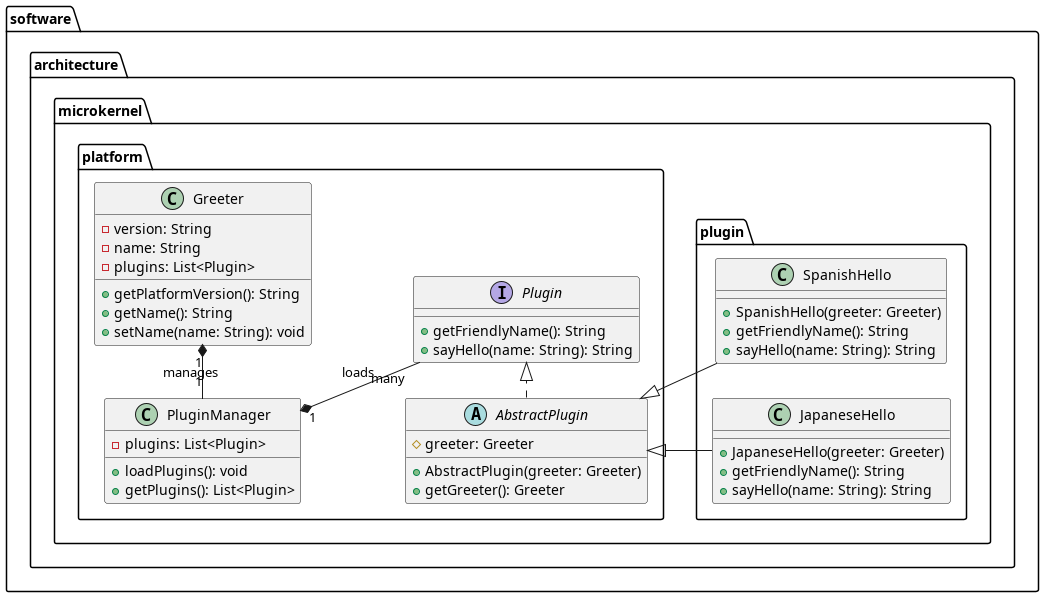
\includegraphics[width=\textwidth]{../images/out/plugin_architecture}
	\caption{Plugin Architecture for Multilingual Greeting App}
	\label{fig:plugin_architecture}
\end{figure}


\subsection{Antarmuka \texttt{Plugin}}

Antarmuka \texttt{Plugin} dalam arsitektur microkernel pada kasus ini berfungsi sebagai kontrak bagi semua plugin yang akan digunakan dalam sistem. Dengan menggunakan antarmuka ini, sistem dapat berinteraksi dengan berbagai implementasi plugin tanpa bergantung pada detail spesifik dari setiap kelas plugin.

\begin{lstlisting}[style=JavaStyle, caption={Antarmuka \texttt{Plugin}}, label={lst:plugin-interface}]
	package software.architecture.microkernel.platform;
	
	public interface Plugin {
		String getFriendlyName();
		String sayHello(String name);
	}
\end{lstlisting}

\noindent
Antarmuka ini mendefinisikan dua metode utama:

\begin{itemize}
	\item \textbf{\texttt{getFriendlyName()}}: Metode ini mengembalikan nama ramah dari plugin, yang dapat digunakan untuk menampilkan informasi mengenai plugin kepada pengguna.
	\item \textbf{\texttt{sayHello(String name)}}: Metode ini menerima sebuah string \texttt{name} dan mengembalikan salam yang telah dikustomisasi berdasarkan implementasi dari plugin.
\end{itemize}

Dengan mendeklarasikan antarmuka ini, setiap plugin yang dikembangkan dalam sistem harus mengimplementasikan metode-metode tersebut, memastikan bahwa semua plugin memiliki fungsionalitas yang konsisten. Ini memungkinkan arsitektur microkernel untuk secara dinamis memuat dan menggunakan plugin yang berbeda tanpa perlu mengetahui detail internalnya.

Penggunaan antarmuka ini mendukung prinsip \textbf{Open/Closed Principle (OCP)} dalam desain perangkat lunak, di mana sistem dapat diperluas dengan menambahkan plugin baru tanpa harus mengubah kode inti dari microkernel.


\subsection{Kelas Abstrak \texttt{AbstractPlugin}}

Kelas abstrak \texttt{AbstractPlugin} merupakan implementasi dasar dari antarmuka \texttt{Plugin}. Kelas ini bertindak sebagai kelas induk bagi semua plugin yang akan digunakan dalam sistem, menyediakan struktur dasar yang diperlukan untuk berinteraksi dengan \texttt{Greeter}.

\begin{lstlisting}[style=JavaStyle, caption={Kelas Abstrak \texttt{AbstractPlugin}}, label={lst:abstract-plugin}]
	package software.architecture.microkernel.platform;
	
	public abstract class AbstractPlugin implements Plugin {
		protected Greeter greeter;
		
		public AbstractPlugin(Greeter greeter) {
			this.greeter = greeter;
		}
	}
\end{lstlisting}

\noindent
Kelas ini memiliki beberapa elemen penting:

\begin{itemize}
	\item \textbf{\texttt{implements Plugin}}: Kelas ini mengimplementasikan antarmuka \texttt{Plugin}, sehingga setiap kelas turunan wajib menyediakan implementasi metode yang didefinisikan dalam \texttt{Plugin}.
	\item \textbf{\texttt{protected Greeter greeter}}: Variabel ini memungkinkan setiap plugin untuk mengakses instance dari \texttt{Greeter}, yang berfungsi sebagai pengelola utama dalam sistem.
	\item \textbf{\texttt{public AbstractPlugin(Greeter greeter)}}: Konstruktor ini menginisialisasi objek \texttt{greeter}, memastikan bahwa setiap plugin yang dibuat memiliki referensi ke \texttt{Greeter}.
\end{itemize}

Dengan menggunakan kelas abstrak ini, pengembang dapat dengan mudah membuat plugin baru dengan hanya mengimplementasikan metode yang didefinisikan dalam \texttt{Plugin}, tanpa harus menangani detail implementasi dasar yang sudah disediakan oleh \texttt{AbstractPlugin}. Hal ini membantu menjaga prinsip \textbf{kode yang dapat digunakan kembali} dan memudahkan perluasan sistem microkernel.


\subsection{Kelas \texttt{SpanishHello}}

Kelas \texttt{SpanishHello} merupakan salah satu implementasi plugin dari sistem microkernel yang bertanggung jawab untuk memberikan salam dalam bahasa Spanyol. Kelas ini mewarisi \texttt{AbstractPlugin}, sehingga memperoleh akses ke objek \texttt{Greeter} yang digunakan dalam platform.

\begin{lstlisting}[style=JavaStyle, caption={Kelas \texttt{SpanishHello}}, label={lst:spanish-hello}]
	package software.architecture.microkernel.plugin;
	
	import software.architecture.microkernel.platform.Greeter;
	import software.architecture.microkernel.platform.AbstractPlugin;
	
	public class SpanishHello extends AbstractPlugin {
		
		public SpanishHello(Greeter greeter) {
			super(greeter);
			System.out.println(getFriendlyName() + " is loaded by Greeter " 
			+ greeter.getPlatformVersion());
		}
		
		@Override
		public String getFriendlyName() {
			return "Greet in Spanish";
		}
		
		@Override
		public String sayHello(String name) {
			return "Hola, " + name + "!";
		}
	}
\end{lstlisting}

\noindent
Kelas ini memiliki beberapa elemen utama:

\begin{itemize}
	\item \textbf{\texttt{extends AbstractPlugin}}: Kelas ini merupakan subclass dari \texttt{AbstractPlugin}, sehingga mendapatkan fungsionalitas dasar dari kelas induk.
	\item \textbf{\texttt{public SpanishHello(Greeter greeter)}}: Konstruktor yang menerima instance dari \texttt{Greeter} sebagai argumen dan meneruskannya ke konstruktor \texttt{AbstractPlugin}. Konstruktor ini juga mencetak pesan bahwa plugin telah berhasil dimuat.
	\item \textbf{\texttt{public String getFriendlyName()}}: Metode ini mengembalikan nama tampilan dari plugin, yaitu \texttt{"Greet in Spanish"}.
	\item \textbf{\texttt{public String sayHello(String name)}}: Metode ini menghasilkan salam dalam bahasa Spanyol dengan format \texttt{"Hola, <name>!"}.
\end{itemize}

Kelas \texttt{SpanishHello} menunjukkan bagaimana sebuah plugin dapat diintegrasikan ke dalam sistem microkernel. Dengan hanya mengimplementasikan metode dari antarmuka \texttt{Plugin}, kelas ini dapat ditambahkan ke dalam sistem tanpa perlu memodifikasi inti dari platform.

\subsection{Kelas \texttt{JapaneseHello}}

Kelas \texttt{JapaneseHello} adalah salah satu implementasi plugin dalam sistem microkernel yang bertanggung jawab untuk memberikan salam dalam bahasa Jepang. Kelas ini mewarisi \texttt{AbstractPlugin}, yang berarti mendapatkan akses ke objek \texttt{Greeter} dari platform.

\begin{lstlisting}[style=JavaStyle, caption={Kelas \texttt{JapaneseHello}}, label={lst:japanese-hello}, inputencoding=utf8]
	package software.architecture.microkernel.plugin;
	
	import software.architecture.microkernel.platform.Greeter;
	import software.architecture.microkernel.platform.AbstractPlugin;
	
	public class JapaneseHello extends AbstractPlugin {
		
		public JapaneseHello(Greeter greeter) {
			super(greeter);
			System.out.println(getFriendlyName() + " is loaded by Greeter " 
			+ greeter.getPlatformVersion());
		}
		
		@Override
		public String getFriendlyName() {
			return "Greet in Japanese";
		}
		
		@Override
		public String sayHello(String name) {
			return "こんにちは, " + name + "!";
		}
	}
\end{lstlisting}




\noindent
Kelas ini memiliki beberapa elemen utama:

\begin{itemize}
	\item \textbf{\texttt{extends AbstractPlugin}}: Kelas ini merupakan subclass dari \texttt{AbstractPlugin}, sehingga mendapatkan fungsionalitas dasar yang sama dengan plugin lainnya.
	\item \textbf{\texttt{public JapaneseHello(Greeter greeter)}}: Konstruktor menerima instance dari \texttt{Greeter} sebagai argumen dan meneruskannya ke konstruktor \texttt{AbstractPlugin}. Selain itu, mencetak pesan bahwa plugin telah berhasil dimuat.
	\item \textbf{\texttt{public String getFriendlyName()}}: Metode ini mengembalikan nama tampilan dari plugin, yaitu \texttt{"Greet in Japanese"}.
	\item \textbf{\texttt{public String sayHello(String name)}}: Metode ini menghasilkan salam dalam bahasa Jepang dengan format \texttt{"こんにちは, <name>!"}.
\end{itemize}

Dengan desain ini, \texttt{JapaneseHello} dapat dimuat secara dinamis oleh sistem microkernel tanpa perlu memodifikasi inti dari platform. Arsitektur ini memungkinkan fleksibilitas tinggi dalam menambahkan dan mengelola plugin.

\subsection{Kelas \texttt{PluginManager}}

Kelas \texttt{PluginManager} bertanggung jawab untuk mengelola siklus hidup plugin dalam arsitektur \textbf{Microkernel}. Kelas ini memungkinkan pemuatan plugin secara dinamis dari direktori eksternal dan memastikan bahwa plugin yang dimuat sesuai dengan antarmuka \texttt{Plugin}. 

\begin{lstlisting}[style=JavaStyle, caption={Kelas \texttt{PluginManager}}, label={lst:plugin-manager}, inputencoding=utf8]
	package software.architecture.microkernel.platform;
	
	import java.io.File;
	import java.io.InputStream;
	import java.lang.reflect.Constructor;
	import java.net.URL;
	import java.net.URLClassLoader;
	import java.util.*;
	
	public class PluginManager {
		
		private final Greeter greeter;
		private final List<Plugin> plugins = new ArrayList<>();
		
		public PluginManager(Greeter greeter) {
			this.greeter = greeter;
		}
		
		public void loadPlugins() {
			try {
				File pluginDir = new File("plugins");
				if (!pluginDir.exists() || !pluginDir.isDirectory()) {
					System.out.println("No plugins directory found.");
					return;
				}
				
				File[] jarFiles = pluginDir.listFiles((dir, name) -> name.endsWith(".jar"));
				if (jarFiles == null || jarFiles.length == 0) {
					System.out.println("No plugins found.");
					return;
				}
				
				for (File jar : jarFiles) {
					URLClassLoader classLoader = new URLClassLoader(new URL[]{jar.toURI().toURL()}, getClass().getClassLoader());
					InputStream propertiesInputStream = classLoader.getResourceAsStream("plugin.properties");
					
					if (propertiesInputStream == null) {
						System.out.println("Missing plugin.properties in " + jar.getName());
						continue;
					}
					
					Properties properties = new Properties();
					properties.load(propertiesInputStream);
					String mainClassName = properties.getProperty("mainclass");
					
					if (mainClassName == null || mainClassName.isEmpty()) {
						System.out.println("Invalid mainclass entry in " + jar.getName());
						continue;
					}
					
					Class<?> classToLoad = Class.forName(mainClassName, true, classLoader);
					Class<? extends Plugin> pluginClass = classToLoad.asSubclass(Plugin.class);
					Constructor<? extends Plugin> constructor = pluginClass.getDeclaredConstructor(Greeter.class);
					Plugin plugin = constructor.newInstance(greeter);
					plugins.add(plugin);
				}
				
			} catch (Exception e) {
				e.printStackTrace();
			}
		}
		
		public List<Plugin> getPlugins() {
			return plugins;
		}
	}
\end{lstlisting}

Kelas ini memiliki beberapa tanggung jawab utama:

\begin{itemize}
	\item \textbf{Memuat plugin dari direktori \texttt{plugins}/} \\
	Fungsi \texttt{loadPlugins()} mencari file \texttt{.jar} dalam direktori \texttt{plugins} dan menggunakan \texttt{URLClassLoader} untuk memuat kelas utama dari plugin.
	
	\item \textbf{Membaca konfigurasi plugin dari \texttt{plugin.properties}} \\
	Setiap plugin harus memiliki file \texttt{plugin.properties} yang menentukan kelas utama plugin dalam entri \texttt{mainclass}. Jika file atau entri ini tidak ditemukan, plugin tidak akan dimuat.
	
	\item \textbf{Menggunakan refleksi untuk menginisialisasi plugin} \\
	Setelah menemukan kelas utama plugin, kelas \texttt{PluginManager} menggunakan mekanisme refleksi untuk membuat instance dari plugin, dengan menyertakan referensi ke objek \texttt{Greeter}.
	
	\item \textbf{Menyimpan daftar plugin yang dimuat} \\
	Semua plugin yang berhasil dimuat akan disimpan dalam daftar \texttt{plugins}, yang dapat diakses melalui metode \texttt{getPlugins()}.
\end{itemize}

Kelas \texttt{PluginManager} adalah komponen kunci dalam arsitektur Microkernel, memungkinkan ekstensi fungsionalitas tanpa harus mengubah kode utama sistem.

\subsection{Kelas \texttt{Greeter}}

Kelas \texttt{Greeter} berfungsi sebagai inti dari platform \textbf{Microkernel} yang bertugas menginisialisasi dan menjalankan sistem. Kelas ini memanfaatkan \texttt{PluginManager} untuk memuat plugin secara dinamis dan menyediakan antarmuka interaktif kepada pengguna untuk memilih dan menjalankan plugin.

\begin{lstlisting}[style=JavaStyle, caption={Kelas \texttt{Greeter}}, label={lst:greeter}, inputencoding=utf8]
	package software.architecture.microkernel.platform;
	
	import java.io.BufferedReader;
	import java.io.InputStreamReader;
	import java.util.List;
	
	public class Greeter {
		
		private final String version = "v1.0.1";
		private String name = "Alice";
		private final PluginManager pluginManager;
		
		public Greeter() {
			this.pluginManager = new PluginManager(this);
			this.pluginManager.loadPlugins();
		}
		
		public static void main(String[] args) {
			Greeter greeter = new Greeter();
			greeter.run();
		}
		
		public void run() {
			try (BufferedReader reader = new BufferedReader(new InputStreamReader(System.in))) {
				while (true) {
					System.out.println("Select the language to greet in:");
					List<Plugin> plugins = pluginManager.getPlugins();
					for (int i = 0; i < plugins.size(); i++) {
						System.out.println((i + 1) + ". " + plugins.get(i).getFriendlyName());
					}
					System.out.println("0. Quit");
					System.out.print("Input: ");
					
					int menu = Integer.parseInt(reader.readLine()) - 1;
					if (menu == -1) break;
					
					if (menu >= 0 && menu < plugins.size()) {
						System.out.println("\n" + plugins.get(menu).sayHello(name) + "\n");
					} else {
						System.out.println("Invalid selection. Try again.");
					}
				}
				
				System.out.println("Quit. Thanks for playing!");
			} catch (Exception e) {
				e.printStackTrace();
			}
		}
		
		public String getPlatformVersion() {
			return version;
		}
		
		public String getName() {
			return name;
		}
	}
\end{lstlisting}

Kelas ini memiliki beberapa tanggung jawab utama:

\begin{itemize}
	\item \textbf{Inisialisasi \texttt{PluginManager}} \\
	Pada konstruktor \texttt{Greeter}, objek \texttt{PluginManager} diinisialisasi dan langsung memanggil metode \texttt{loadPlugins()} untuk memuat plugin yang tersedia.
	
	\item \textbf{Menyediakan antarmuka interaktif pengguna} \\
	Metode \texttt{run()} bertanggung jawab menampilkan daftar plugin yang tersedia dan meminta input dari pengguna untuk memilih plugin yang akan dijalankan.
	
	\item \textbf{Menghubungkan plugin dengan sistem utama} \\
	Saat pengguna memilih plugin, \texttt{Greeter} akan memanggil metode \texttt{sayHello()} dari plugin tersebut, dengan menyertakan nama pengguna.
	
	\item \textbf{Menyediakan informasi platform} \\
	Metode \texttt{getPlatformVersion()} dan \texttt{getName()} digunakan oleh plugin untuk mengakses informasi tentang platform dan nama pengguna.
\end{itemize}

Kelas \texttt{Greeter} berfungsi sebagai pusat kendali dalam arsitektur Microkernel, memungkinkan ekstensi fungsionalitas melalui plugin tanpa memerlukan perubahan pada inti aplikasi. Sistem ini dirancang agar mudah diperluas dan modular.


\section{Kompilasi dan Menjalankan Aplikasi}

Aplikasi berbasis \textbf{Microkernel} ini menggunakan \textbf{Maven} sebagai alat bantu untuk membangun (\textit{build}) dan mengelola dependensi. Proses kompilasi dan eksekusi dilakukan dalam dua tahap utama:

\begin{enumerate}
	\item Membangun (\textit{package}) proyek platform utama (\texttt{Greeter}).
	\item Membangun setiap plugin sebagai proyek Maven yang terpisah.
	\item Memindahkan berkas \texttt{.jar} hasil kompilasi plugin ke dalam folder \texttt{plugins} pada proyek platform.
	\item Menjalankan aplikasi platform, yang secara otomatis memuat semua plugin yang tersedia.
\end{enumerate}

\subsection{Membangun dan Menginstal Proyek Platform}

Untuk membangun proyek utama yang berisi \texttt{Greeter}, jalankan perintah berikut di dalam direktori proyek \textbf{platform}:

\begin{lstlisting}[language=bash, caption={Membangun Proyek Platform Menggunakan Maven}]
	mvn clean package install
\end{lstlisting}

Setelah perintah ini dijalankan, Maven akan:

\begin{itemize}
	\item Mengunduh dan mengelola semua dependensi yang diperlukan.
	\item Mengkompilasi kode sumber platform.
	\item Menghasilkan berkas \texttt{.jar} di dalam direktori \texttt{target/}.
\end{itemize}

\subsection{Membangun Plugin}

Setiap plugin, seperti \texttt{JapaneseHello} dan \texttt{SpanishHello}, harus dikompilasi dan dikemas sebagai \texttt{.jar} secara terpisah. Untuk membangun setiap plugin, navigasikan ke direktori masing-masing plugin dan jalankan:

\begin{lstlisting}[language=bash, caption={Membangun Plugin Menggunakan Maven}]
	mvn clean package 
\end{lstlisting}

Hasil kompilasi akan berada di dalam direktori \texttt{target/} dengan nama sesuai konfigurasi \texttt{pom.xml}.

\subsection{Memindahkan Plugin ke Direktori \texttt{plugins}}

Setelah semua plugin berhasil dikompilasi dan dikemas sebagai \texttt{.jar}, langkah berikutnya adalah memindahkan berkas-berkas tersebut ke dalam folder \texttt{plugins} yang ada di dalam proyek \textbf{platform}. Gunakan perintah berikut untuk memindahkan hasil kompilasi:

\begin{lstlisting}[language=bash, caption={Memindahkan Plugin ke Direktori \texttt{plugins}}]
	mv target/*.jar ../platform/plugins/
\end{lstlisting}

\subsection{Menjalankan Aplikasi Platform}

Setelah semua plugin berada dalam direktori \texttt{plugins}, aplikasi \texttt{Greeter} dapat dijalankan. Sistem akan secara otomatis memuat semua plugin yang tersedia dan menampilkannya dalam daftar pilihan bahasa. Jalankan aplikasi menggunakan perintah:

\begin{lstlisting}[language=bash, caption={Menjalankan Aplikasi Platform}]
	mvn run 
	# atau
	java -jar target/platform.jar
\end{lstlisting}

\subsection{Output Program}

Jika semua langkah telah dilakukan dengan benar, aplikasi akan menampilkan output berikut:

\begin{lstlisting}[language=bash, caption={Contoh Output Saat Menjalankan Aplikasi}]
	Greet in Japanese is loaded by Greeter v1.0.1
	Greet in Spanish is loaded by Greeter v1.0.1
	Select the language to greet in:
	1. Greet in Japanese
	2. Greet in Spanish
	0. Quit
	Input: 1
	
	XXXXX, Alice!
	
	Select the language to greet in:
	1. Greet in Japanese
	2. Greet in Spanish
	0. Quit
	Input: 2
	
	Hola, Alice!
	
	Select the language to greet in:
	1. Greet in Japanese
	2. Greet in Spanish
	0. Quit
	Input:
\end{lstlisting}

Dengan pendekatan ini, sistem dapat memuat plugin secara dinamis tanpa perlu melakukan perubahan atau kompilasi ulang pada kode sumber utama. Setiap plugin cukup dikompilasi secara terpisah dan ditambahkan ke direktori \texttt{plugins}, menjadikan arsitektur ini fleksibel dan modular.


\section{Kesimpulan}

Arsitektur \textbf{microkernel} dan \textbf{plugin} merupakan dua pendekatan yang digunakan untuk meningkatkan modularitas, fleksibilitas, dan skalabilitas dalam pengembangan perangkat lunak. Microkernel memungkinkan pemisahan layanan sistem dari kernel utama, sehingga meningkatkan keamanan dan ketahanan terhadap kegagalan. Sementara itu, plugin architecture memberikan fleksibilitas dengan memungkinkan ekstensi fungsionalitas tanpa mengubah kode inti sistem.

Meskipun microkernel menawarkan keunggulan dalam stabilitas dan keamanan, pendekatan ini memiliki tantangan dalam hal efisiensi komunikasi antar-proses dan kompleksitas implementasi. Oleh karena itu, penerapan microkernel lebih umum digunakan dalam sistem yang membutuhkan keandalan tinggi seperti sistem tertanam, sistem operasi real-time, dan hypervisor virtualisasi.

Di sisi lain, plugin architecture banyak digunakan dalam aplikasi perangkat lunak yang membutuhkan kemampuan ekspansi, seperti Integrated Development Environment (IDE), sistem manajemen konten (CMS), dan mesin game. Dengan menggunakan pendekatan ini, pengembang dapat memperluas fungsionalitas perangkat lunak tanpa perlu mengubah kode sumber utama, sehingga meningkatkan skalabilitas dan kemudahan pemeliharaan.

Melalui implementasi berbasis Java, dokumen ini telah menunjukkan bagaimana microkernel dan plugin dapat diterapkan dalam praktik, termasuk teknik pemuatan dinamis plugin menggunakan refleksi dan manajemen dependensi dengan Maven. Pendekatan ini memungkinkan pengembangan sistem yang lebih modular, terstruktur, dan mudah diperluas.

Dengan pemahaman yang lebih mendalam mengenai arsitektur microkernel dan plugin, pengembang dapat memilih strategi yang paling sesuai dengan kebutuhan sistem yang sedang dibangun. Baik untuk pengembangan sistem operasi maupun aplikasi perangkat lunak modern, kedua arsitektur ini tetap menjadi solusi utama dalam menciptakan sistem yang lebih fleksibel dan tangguh terhadap perubahan.


%\chapter{Pipe-and-Filter}
\authors{Alfa Yohannis, Rizki Wahyudi, Tommy Chitiawan, Mandalan}


	%\gny{Tolong tambahkan keterangan gambar contoh : Gambar 7.1, 7.2, dst.. dan tambahkan italic text untuk setiap bahasa asing}

	\section{Definisi}
		\textit{Pipe and Filter Architecture} adalah sebuah pendekatan desain perangkat lunak yang menggambarkan bagaimana data dapat diproses melalui serangkaian \textit{filter} atau pemroses yang saling terkait dan saling bergantung dalam suatu \textit{pipeline}. Setiap \textit{filter} memiliki tugas spesifik untuk mengubah atau memanipulasi data yang melewatinya, dan data tersebut kemudian dikirim ke \textit{filter} berikutnya dalam \textit{pipeline} untuk diproses lebih lanjut.
	
	\textit{Pipe and Filter Architecture} terdiri dari beberapa elemen utama, yaitu:
	\begin{itemize}
		\item \textit{Pipes}: adalah saluran yang menghubungkan antara satu \textit{filter} dengan \textit{filter} lainnya. Pipe digunakan untuk mengalirkan data dari satu \textit{filter} ke \textit{filter} berikutnya.
		\item \textit{filter}: adalah blok bangunan logika yang bertanggung jawab untuk memproses dan mengubah data. \textit{Filter} dapat melakukan tugas sederhana seperti memisahkan atau menyaring data, atau tugas yang lebih kompleks seperti mengubah format data.
		\item \textit{Source dan Sink}: adalah elemen yang menghasilkan \textit{input} data dan menerima \textit{output} data dari \textit{pipeline}.
	\end{itemize}
	
	Keuntungan utama dari \textit{Pipe and Filter Architecture} adalah bahwa ia memungkinkan pengembang untuk membangun sistem yang sangat modular, dengan setiap \textit{filter} melakukan tugas yang jelas dan terbatas. Hal ini membuat perubahan pada pipeline lebih mudah dan aman, karena hanya memerlukan perubahan pada satu \textit{filter} tanpa mempengaruhi \textit{filter} lainnya. Selain itu, arsitektur ini juga dapat meningkatkan kinerja sistem, karena memungkinkan untuk memproses data secara paralel dalam beberapa \textit{filter}.
	
	Namun, kelemahan dari \textit{Pipe and Filter Architecture} adalah bahwa dapat menjadi sulit untuk menangani kasus penggunaan yang kompleks, karena setiap filter harus dirancang dengan sangat baik agar dapat berjalan dengan benar dalam pipeline. Selain itu, pengembang harus memperhatikan antarmuka antara filter yang berbeda agar dapat saling berinteraksi dengan benar.
	
	
	\section{\textit{Pipe and Filter Architecture Schema}}
		\begin{figure}[h] 
		\begin{center} 
			\renewcommand{\figurename}{Gambar} 
			\includegraphics[scale=0.5]{Capture.png} 
			\caption{\textit{pipe and filter}} 
			\label{gambar} 
		\end{center} 
	\end{figure}
	
	\section{Kelebihan}
	
	\begin{itemize}
		\item Memastikan sambungan komponen, \textit{filter} yang longgar dan fleksibel.
		\item Kopling longgar memungkinkan \textit{filter} diubah tanpa modifikasi ke \textit{filter} lain.
		\item Konduktif untuk pemrosesan paralel.
		\item\textit{filter} dapat diperlakukan sebagai kotak hitam. Pengguna sistem tidak perlu mengetahui logika di balik kerja setiap \textit{filter}.
		\item Dapat digunakan kembali. Setiap \textit{filter} dapat dipanggil dan digunakan berulang kali.
	\end{itemize}
	
	
	\section{Kekurangan}
	
	\begin{itemize}
		\item Penambahan sejumlah besar \textit{filter independent} dapat mengurangi kinerja karena overhead komputasi yang berlebihan.
		\item Bukan pilihan yang baik untuk sistem interaktif.
		\item Sistem \textit{pipe and filter} mungkin tidak cocok untuk perhitungan jangka panjang.
		
	\section{penerapan dalam aplikasi}
		\begin{itemize}
			\item Sistem pengolahan data: \textit{Pipe and filter} dapat digunakan untuk mengambil data dari berbagai sumber dan memprosesnya melalui serangkaian \textit{filter} untuk menghasilkan \textit{output} yang diinginkan.
			
			\item Sistem pengolahan gambar: \textit{Pipe and filter} dapat digunakan untuk memproses gambar atau video yang diambil dari kamera dengan menggunakan berbagai filter untuk menghasilkan gambar yang lebih baik atau memberikan efek khusus.
			
			\item Sistem pencarian: \textit{Pipe and filter} dapat digunakan untuk memproses data pencarian yang diberikan oleh pengguna dan memfilter data untuk menghasilkan hasil pencarian yang relevan.
			
			\item Sistem pemrosesan audio: \textit{Pipe and filter} dapat digunakan untuk memproses audio dan melakukan pengolahan suara seperti pengurangan kebisingan, pengaturan volume, dan pemotongan audio.
			
			\item Sistem pemrosesan teks: \textit{Pipe and filter} dapat digunakan untuk memproses teks dan melakukan pengolahan bahasa alami seperti analisis sentimen dan pengenalan entitas.
		\end{itemize}
	\end{itemize}


%\chapter{Space-based Architecture}

\section{Pendahuluan}

Space-based architecture merupakan salah satu pendekatan arsitektur perangkat lunak yang dirancang untuk menghadapi tantangan skalabilitas, ketersediaan, dan performa tinggi pada sistem modern. Dalam dunia yang semakin mengandalkan pemrosesan data secara real-time dan sistem yang responsif terhadap lonjakan beban secara tiba-tiba, pendekatan tradisional seperti arsitektur monolitik atau client-server sering kali menemui keterbatasan. Space-based architecture muncul sebagai solusi yang memanfaatkan prinsip in-memory computing dan komunikasi melalui media data bersama (space) untuk menghindari bottleneck dan mempercepat akses data.

Tujuan utama dari penggunaan arsitektur ini adalah untuk menciptakan sistem yang elastis, tangguh, dan mampu diskalakan secara horizontal. Dengan mengandalkan unit pemrosesan yang independen (processing units) dan data grid yang terdistribusi, space-based architecture memungkinkan sistem untuk menyesuaikan kapasitasnya sesuai dengan beban kerja yang berubah-ubah. Hal ini sangat penting dalam konteks aplikasi yang mengalami traffic dinamis, seperti layanan pemesanan online, perbankan digital, dan sistem analisis data real-time.

Masalah utama yang ingin diselesaikan oleh space-based architecture adalah terjadinya bottleneck pada titik-titik tertentu dalam sistem, seperti database pusat atau load balancer tunggal. Selain itu, pendekatan ini juga mengatasi isu latensi tinggi akibat pemrosesan yang terfokus pada satu titik pusat. Dengan mendistribusikan beban kerja dan data secara merata ke seluruh unit dalam sistem, space-based architecture mengurangi ketergantungan pada komponen pusat dan meningkatkan ketersediaan sistem secara keseluruhan.

Pendekatan ini juga sejalan dengan prinsip desain modern dalam pengembangan sistem berskala besar, termasuk prinsip loose coupling, elastic scalability, dan fault tolerance. Oleh karena itu, space-based architecture menjadi salah satu pilihan strategis dalam merancang sistem yang handal, responsif, dan mampu bertahan dalam lingkungan operasional yang dinamis dan kompleks.

\section{Sejarah}

Konsep space-based architecture berakar dari kebutuhan akan sistem yang mampu menangani beban kerja tinggi dan bersifat elastis tanpa mengalami hambatan kinerja pada titik-titik pusat sistem. Gagasan dasarnya terinspirasi dari model blackboard architecture dalam kecerdasan buatan, di mana berbagai komponen independen dapat membaca dan menulis ke papan informasi bersama untuk menyelesaikan permasalahan secara kolektif. Pendekatan ini kemudian diadaptasi ke dalam konteks sistem perangkat lunak terdistribusi dengan menekankan pada penggunaan media penyimpanan bersama sebagai pusat interaksi data, yang dikenal sebagai \textit{space}.

Pada awal tahun 2000-an, pertumbuhan aplikasi berbasis web dan kebutuhan terhadap sistem yang selalu aktif (\textit{always-on}) memicu lahirnya teknologi in-memory data grid (IMDG), yaitu mekanisme penyimpanan data di dalam memori yang dapat diakses secara paralel oleh banyak proses. Teknologi ini mendukung ide untuk membangun sistem yang tidak lagi bergantung pada database relasional sebagai pusat penyimpanan data, melainkan menyebarkan data ke seluruh node dalam bentuk grid. Hal ini mempercepat akses dan pemrosesan data secara signifikan.

Salah satu pelopor utama dalam implementasi arsitektur ini adalah GigaSpaces Technologies, yang memperkenalkan produk XAP (eXtreme Application Platform). Platform ini menggabungkan konsep processing unit, space, dan middleware virtualisasi untuk membangun sistem yang sepenuhnya terdistribusi. Keberhasilan GigaSpaces dalam mendukung sistem pemrosesan transaksi berskala besar mendorong munculnya platform serupa seperti Oracle Coherence dan Hazelcast, yang juga mengadopsi pendekatan space-based.

Seiring waktu, space-based architecture mulai mendapatkan perhatian dalam komunitas pengembang perangkat lunak dan perusahaan teknologi karena kemampuannya dalam menangani kebutuhan sistem yang bersifat \textit{elastic}, \textit{resilient}, dan \textit{scalable}. Dengan kemajuan teknologi seperti containerization, orchestrator seperti Kubernetes, serta peningkatan kapasitas memori dan jaringan, penerapan arsitektur ini menjadi semakin relevan dalam pengembangan sistem modern yang berorientasi pada performa tinggi dan toleransi terhadap kegagalan.

\section{Penerapan}

Space-based architecture telah digunakan secara luas dalam berbagai konteks aplikasi yang memerlukan skalabilitas tinggi dan waktu respons yang rendah. Salah satu penerapan paling nyata adalah pada sistem e-commerce berskala besar. Dalam skenario seperti promosi besar-besaran, flash sale, atau hari belanja nasional, sistem e-commerce sering menghadapi lonjakan trafik secara tiba-tiba yang dapat menyebabkan server kelebihan beban dan bahkan gagal beroperasi. Dengan menggunakan space-based architecture, setiap permintaan dari pengguna dapat dimasukkan ke dalam \textit{space} dan diproses oleh unit-unit pemrosesan (processing unit) secara paralel, sehingga beban sistem terdistribusi secara merata dan tidak menimbulkan bottleneck pada satu titik.

Selain itu, space-based architecture juga sangat cocok diterapkan pada aplikasi yang berbasis waktu nyata (real-time) dan berbasis event (event-driven). Contohnya adalah dalam sistem notifikasi push, layanan streaming, atau pemantauan sistem secara langsung. Dengan memanfaatkan space sebagai kanal komunikasi dan penyimpanan data yang bersifat sementara, sistem dapat bereaksi terhadap peristiwa yang terjadi dengan latensi yang sangat rendah. Proses asinkron dan pemrosesan paralel menjadi sangat mudah diterapkan, karena tidak memerlukan koordinasi yang kompleks antar komponen.

Integrasi space-based architecture dengan teknologi cloud dan arsitektur microservices juga menunjukkan sinergi yang kuat. Dalam konteks cloud, space dapat tersebar di berbagai zona ketersediaan (availability zones) untuk menjamin ketahanan data dan kesinambungan layanan. Sementara itu, dalam pendekatan microservices, setiap layanan mikro dapat berinteraksi dengan space tanpa saling tergantung secara langsung, yang membantu mengurangi keterkaitan antar layanan dan meningkatkan fleksibilitas dalam pengembangan serta deployment. Kombinasi ini menghasilkan sistem yang dapat diatur, diukur, dan diperluas secara dinamis sesuai kebutuhan, tanpa perlu mengorbankan keandalan atau performa sistem.

Dengan demikian, penerapan space-based architecture terbukti sangat relevan dalam membangun sistem modern yang menuntut kecepatan, keandalan, dan skalabilitas, baik dalam lingkungan lokal maupun berbasis cloud.


\section{Keunggulan}

Space-based architecture menawarkan sejumlah keunggulan signifikan dibandingkan pendekatan arsitektur tradisional, terutama dalam konteks aplikasi yang memerlukan performa tinggi, skalabilitas, dan ketersediaan sistem yang konsisten. Keunggulan-keunggulan ini menjadikan space-based architecture sebagai solusi strategis untuk sistem berskala besar dan bersifat dinamis. Berikut adalah tiga keunggulan utama yang paling menonjol:

\begin{enumerate}
	\item \textbf{Skalabilitas Horizontal.}  
	Dalam arsitektur ini, unit pemrosesan (\textit{processing unit}) dapat ditambahkan atau dikurangi secara dinamis tanpa memengaruhi kinerja sistem secara keseluruhan. Setiap unit bekerja secara independen dan terhubung ke \textit{space} yang terdistribusi, sehingga tidak ada ketergantungan terhadap titik pusat yang dapat menjadi bottleneck. Dengan demikian, ketika terjadi lonjakan trafik atau permintaan, sistem dapat menskalakan kapasitasnya hanya dengan menambahkan node baru ke dalam cluster tanpa downtime atau konfigurasi ulang yang kompleks.
	
	\item \textbf{Ketersediaan Tinggi (High Availability).}  
	Karena tidak bergantung pada satu titik pusat seperti database tunggal atau load balancer statis, space-based architecture mampu menjaga operasional sistem meskipun terjadi kegagalan pada sebagian komponen. Data yang disimpan secara in-memory dan disebar ke beberapa node dapat direplikasi secara otomatis. Jika salah satu node mengalami gangguan, data tetap tersedia dari node lainnya. Hal ini menjadikan arsitektur ini sangat ideal untuk aplikasi kritikal yang harus selalu aktif dan tidak boleh mengalami waktu henti.
	
	\item \textbf{Performa Melalui In-Memory Processing.}  
	Space-based architecture unggul berkat pemanfaatan in-memory data grid untuk menyimpan seluruh status, objek bisnis, dan pesan komunikasi antar komponen. Karena pengolahan data dilakukan langsung di dalam memori utama, waktu akses dan pemrosesan dapat berlangsung dalam skala milidetik atau bahkan mikrodetik. Pendekatan ini memungkinkan sistem menangani beban transaksi yang sangat tinggi dengan latensi rendah, menjadikannya cocok untuk aplikasi real-time seperti sistem finansial, analitik data cepat, atau pemantauan sensor secara langsung.
\end{enumerate}

Ketiga keunggulan tersebut—skalabilitas horizontal, ketersediaan tinggi, dan performa tinggi—berkontribusi secara signifikan terhadap ketangguhan dan efisiensi space-based architecture sebagai fondasi untuk membangun sistem modern yang fleksibel, andal, dan mampu berkembang sesuai kebutuhan bisnis.



\section{Kelemahan}

Meskipun space-based architecture menawarkan berbagai keunggulan dalam hal skalabilitas, ketersediaan, dan performa, pendekatan ini juga memiliki sejumlah kelemahan yang perlu dipertimbangkan secara matang sebelum diimplementasikan. Beberapa tantangan utama terkait dengan kompleksitas teknis, kebutuhan sumber daya, serta aspek konsistensi dan replikasi data dalam lingkungan terdistribusi. Berikut ini adalah tiga kelemahan utama dari space-based architecture:

\begin{enumerate}
	\item \textbf{Kompleksitas Pengelolaan.}  
	Space-based architecture melibatkan banyak komponen yang bekerja secara paralel dan berkoordinasi melalui \textit{space}. Hal ini berbeda dengan arsitektur monolitik atau client-server yang umumnya bersifat linear dan lebih mudah dipantau. Implementasi space-based membutuhkan perencanaan sistem yang matang, strategi pengelolaan beban kerja yang efisien, serta pemahaman teknis yang mendalam mengenai komunikasi asinkron dan manajemen komponen terdistribusi. Tantangan juga muncul dalam proses debugging, monitoring, dan pemeliharaan sistem karena perilaku komponen yang tersebar dan tidak selalu deterministik.
	
	\item \textbf{Kebutuhan Memori yang Besar.}  
	Karena space-based architecture bergantung pada penyimpanan dan pemrosesan data secara langsung di memori (RAM), kebutuhan terhadap kapasitas memori menjadi sangat tinggi. Semua status sistem, objek bisnis, dan antrian pesan disimpan di memori utama, bukan di media penyimpanan konvensional seperti hard disk. Hal ini memang memberikan kecepatan yang tinggi, namun di sisi lain menuntut investasi hardware yang signifikan, baik dari sisi kapasitas RAM maupun biaya operasionalnya. Dalam skenario skala besar, keterbatasan fisik dan konsumsi energi juga menjadi tantangan tersendiri.
	
	\item \textbf{Kesulitan Replikasi dan Konsistensi Data.}  
	Dalam sistem yang terdistribusi dan bersifat asinkron, menjaga konsistensi data antar node bukanlah tugas yang mudah. Tidak adanya pengelola data pusat berarti setiap node harus memiliki mekanisme replikasi dan sinkronisasi sendiri. Jika tidak ditangani dengan baik, potensi terjadinya konflik data, inkonsistensi, atau bahkan kehilangan data menjadi sangat tinggi. Strategi seperti \textit{eventual consistency}, \textit{versioning}, atau \textit{distributed locking} harus diterapkan dengan hati-hati. Kompleksitas ini semakin meningkat ketika sistem dijalankan dalam lingkungan multi-region atau hybrid cloud, yang memiliki karakteristik latensi dan kegagalan yang berbeda-beda.
\end{enumerate}

Dengan mempertimbangkan ketiga kelemahan tersebut, penerapan space-based architecture membutuhkan kesiapan dari segi perencanaan teknis, alokasi sumber daya, serta kompetensi tim pengembang. Evaluasi menyeluruh terhadap kebutuhan dan karakteristik sistem sangat penting agar pendekatan ini benar-benar memberikan manfaat optimal tanpa menimb


\section{Topology dan Komponen}
Arsitektur Space-Based Architecture memiliki struktur topologi (Gambar \ref{fig:space-based_architecture}) yang tersusun atas berbagai komponen terdistribusi yang bekerja secara paralel dan saling terkoordinasi. Topologi ini dirancang untuk mendukung prinsip skalabilitas horizontal, ketahanan terhadap kegagalan, serta kinerja tinggi melalui pemrosesan data di dalam memori dan replikasi data antar node. Setiap komponen memiliki peran spesifik yang saling melengkapi dalam membangun sistem yang tangguh, fleksibel, dan responsif terhadap beban kerja yang dinamis. Gambar berikut menyajikan ilustrasi dari topologi umum arsitektur ini, diikuti dengan penjelasan masing-masing komponennya.


\begin{figure}[h]
	\centering
	\includegraphics[width=.9\textwidth]{../images/spaced-based\_architecture.jpg}
	\caption{Space-based Architecture}
	\label{fig:space-based_architecture}
\end{figure}

\begin{itemize}
	\item \textbf{Processing Unit (PU)}: Unit pemrosesan yang menggabungkan logika aplikasi (web dan backend) serta data yang dibutuhkan. PU dapat direplikasi dan dipartisi untuk skalabilitas dan toleransi terhadap kegagalan. Setiap PU bekerja secara independen dan memiliki cache data-nya sendiri.
	
	\item \textbf{In-Memory Data Grid Cache}: Penyimpanan data sementara yang berada di dalam memori dan digunakan oleh PU untuk mempercepat akses data. Cache ini menggantikan ketergantungan langsung terhadap database dalam pemrosesan utama.
	
	\item \textbf{Data Replication Engine}: Komponen dalam PU yang bertugas mereplikasi data antar PU untuk menjaga konsistensi dan ketersediaan data di dalam in-memory grid secara terdistribusi.
	
	\item \textbf{Virtualized Middleware}: Lapisan infrastruktur yang menyediakan layanan bersama untuk seluruh arsitektur. Middleware ini menangani orkestrasi proses, penyaluran pesan, sinkronisasi data, dan pengelolaan deployment unit pemrosesan.
	
	\item \textbf{Processing Grid}: Bagian dari middleware yang bertanggung jawab mengoordinasikan eksekusi permintaan yang melibatkan lebih dari satu PU. Ini memastikan bahwa tugas dapat diselesaikan secara paralel dan efisien.
	
	\item \textbf{Messaging Grid}: Komponen yang menerima permintaan masuk dan menentukan PU aktif mana yang harus menangani permintaan tersebut. Fungsinya mirip load balancer tetapi dalam konteks sistem terdistribusi.
	
	\item \textbf{Data Grid}: Sistem memori terdistribusi yang bertindak sebagai ruang bersama (tuple space) untuk menyimpan dan menyinkronkan data antar PU. Data grid dapat dipartisi dan direplikasi untuk skalabilitas dan ketersediaan tinggi.
	
	\item \textbf{Deployment Manager}: Komponen yang bertanggung jawab untuk menyalakan atau mematikan PU berdasarkan kebutuhan beban sistem. Deployment manager memastikan sistem dapat menyesuaikan kapasitas secara elastis.
	
	\item \textbf{Data Pump}: Komponen yang menjembatani antara PU dan database. Ia bertugas mengirimkan pembaruan data dari PU ke database secara asinkron, mendukung prinsip eventual consistency.
	
	\item \textbf{Data Reader}: Komponen yang membaca data dari database dan mengirimkannya ke PU, biasanya hanya digunakan saat pemulihan sistem atau redeploy cache seluruh PU.
	
	\item \textbf{Data Writer}: Komponen yang menerima data dari data pump dan menuliskannya ke database sebagai bentuk persistensi.
	
	\item \textbf{Database}: Sistem penyimpanan utama dan akhir (system of record) untuk seluruh data aplikasi. Pada arsitektur ini, database tidak diakses secara langsung dalam alur utama melainkan diperbarui secara eventual melalui data writer.
\end{itemize}

Pada arsitektur Space-Based Architecture, alur permintaan dimulai dari klien yang mengirimkan request melalui web gateway atau load balancer. Permintaan tersebut kemudian diteruskan ke lapisan \texttt{virtualized middleware}, khususnya ke \texttt{messaging grid}, yang berfungsi menentukan unit pemrosesan (\texttt{processing unit}, \texttt{PU}) aktif yang akan menangani permintaan tersebut. Setelah \texttt{PU} ditentukan, permintaan diproses secara independen oleh \texttt{PU} tersebut.

Setiap \texttt{PU} merupakan entitas mandiri yang menggabungkan komponen logika aplikasi (baik web maupun backend), cache data in-memory melalui \texttt{in-memory data grid}, serta mesin replikasi data. \texttt{PU} menggunakan data dari \texttt{shared memory space}, yang dibangun di atas \texttt{data grid} terdistribusi, untuk mempercepat akses dan menjaga konsistensi antar node. \texttt{PU} dapat membaca dan menulis data ke \texttt{data grid} tanpa perlu bergantung langsung pada \texttt{database}.

Jika selama pemrosesan terjadi pembaruan data, \texttt{PU} yang memproses permintaan tersebut bertindak sebagai pemilik data terbaru. \texttt{PU} kemudian meneruskan pembaruan tersebut melalui \texttt{data pump}, yang bertugas menyampaikan informasi ke \texttt{data writer}. \texttt{Data writer} kemudian menyimpan data ke dalam sistem \texttt{database} secara asynchronous. Di sisi lain, \texttt{data reader} digunakan hanya dalam kondisi tertentu, seperti saat semua \texttt{PU} mengalami kegagalan atau ketika diperlukan sinkronisasi ulang cache, untuk membaca data dari \texttt{database} dan mengirimkannya ke \texttt{PU}.

Untuk mendukung skalabilitas dan elastisitas, \texttt{deployment manager} secara dinamis dapat menambah atau mengurangi jumlah \texttt{PU} sesuai dengan beban sistem. Dengan demikian, arsitektur ini mampu menangani jutaan permintaan secara paralel dengan tingkat toleransi kesalahan yang tinggi, performa cepat, dan fleksibilitas pengelolaan sumber daya.


\section{Aplikasi Sederhana}
\subsection{Desain Aplikasi Parallel Processing}
\subsection{Simulasi Pemrosesan Order}
\subsection{Pengelolaan State dan Status Order}

\section{Kesimpulan}
\subsection{Ringkasan Keunggulan dan Kelemahan}
\subsection{Potensi Implementasi di Masa Depan}
\subsection{Rekomendasi untuk Penggunaan Arsitektur Ini}

%\chapter{Pipe-and-Filter / Pipeline Architecture}

\section{Pendahuluan}

Dalam pengembangan perangkat lunak modern, kebutuhan akan sistem yang modular, mudah dipelihara, dan mampu menangani aliran data secara efisien semakin meningkat. Salah satu pendekatan arsitektur yang dirancang untuk memenuhi kebutuhan tersebut adalah \textbf{Pipe-and-Filter} atau \textbf{Pipeline Architecture}. Arsitektur ini telah banyak digunakan dalam berbagai domain, mulai dari kompilator, pemrosesan data multimedia, hingga sistem big data yang membutuhkan pemrosesan bertahap dalam skala besar. Konsep dasar arsitektur ini yang memisahkan tanggung jawab ke dalam unit-unit terpisah (filter) yang terhubung melalui saluran data (pipe), memberikan fleksibilitas tinggi dalam perancangan sistem, serta mendukung pemrosesan paralel dan streaming secara efisien.

Bab ini bertujuan untuk menjelaskan prinsip dasar, komponen utama, serta pola kerja dari \textbf{Pipe-and-Filter Architecture}. Selain itu, akan dibahas pula contoh penerapan nyata dalam berbagai konteks aplikasi, kelebihan dan kekurangan pendekatan ini, serta bagaimana arsitektur ini dapat diimplementasikan secara sederhana. Pembahasan akan difokuskan pada pemahaman konseptual dan aplikatif tanpa mengeksplorasi terlalu dalam aspek teknis seperti pengoptimalan performa atau integrasi dengan arsitektur kompleks lainnya. Dengan demikian, bab ini diharapkan dapat memberikan fondasi yang kuat untuk memahami bagaimana arsitektur \textbf{pipe-and-filter} dapat digunakan dalam pengembangan sistem perangkat lunak yang modular dan scalable.


\section{Contoh Penerapan}

Salah satu penerapan paling klasik dari arsitektur \textbf{pipe-and-filter} adalah dalam pemrosesan teks, seperti pada kompilator. Sebuah kompilator umumnya terdiri dari serangkaian tahap seperti lexical analysis, parsing, semantic analysis, hingga code generation, yang masing-masing dapat direpresentasikan sebagai filter dalam pipeline. Data dalam bentuk kode sumber akan melewati setiap tahap tersebut secara berurutan untuk menghasilkan output berupa kode mesin atau bytecode. Selain kompilator, pipeline juga digunakan dalam aplikasi text processing, seperti pemfilteran email, analisis log, atau sistem ekstraksi informasi, di mana teks mentah diproses secara bertahap hingga menjadi informasi yang terstruktur.

Dalam bidang multimedia, arsitektur ini digunakan untuk pemrosesan sinyal audio dan video. Contohnya, dalam aplikasi pemutar video, aliran data video mentah mungkin akan melalui beberapa filter seperti dekoder, scaler, dan renderer, sebelum akhirnya ditampilkan ke layar. Demikian pula, dalam aplikasi pengolahan suara, sinyal audio dapat melalui tahap-tahap seperti filtering noise, normalisasi volume, dan kompresi. Setiap tahap bertanggung jawab pada satu tugas pemrosesan spesifik dan bekerja secara independen terhadap input dan output-nya.

Dalam skala yang lebih besar, arsitektur \textbf{pipe-and-filter} juga banyak diterapkan pada sistem big data dan pemrosesan data real-time. Contohnya terdapat pada pipeline ETL (Extract, Transform, Load), di mana data diambil dari berbagai sumber, dibersihkan dan ditransformasi, lalu dimuat ke dalam data warehouse atau sistem analitik. Selain itu, dalam arsitektur data streaming seperti Apache Kafka atau Apache Flink, aliran data dikirim dari satu filter ke filter lainnya untuk diproses secara kontinu dan paralel, mendukung sistem yang skalabel dan responsif. Penerapan seperti ini menunjukkan bagaimana prinsip \textbf{pipe-and-filter} dapat diadaptasi dalam lingkungan komputasi modern dengan volume data yang besar dan sesuai kebutuhan.


\section{Kelebihan dan Kekurangan}

Arsitektur \textbf{pipe-and-filter} memiliki sejumlah kelebihan yang menjadikannya pilihan yang menarik dalam berbagai konteks pengembangan sistem. Beberapa keunggulan utamanya antara lain:

\begin{enumerate}
	\item \textbf{Modularitas}: Setiap filter dirancang untuk menjalankan satu tugas spesifik secara independen, sehingga memudahkan proses pengembangan, pengujian, dan pemeliharaan. Perubahan pada satu filter tidak memengaruhi filter lainnya selama antarmuka tetap konsisten.
	
	\item \textbf{Reusabilitas}: Komponen filter yang telah dikembangkan dapat digunakan kembali dalam pipeline atau sistem lain, tanpa perlu modifikasi besar. Hal ini meningkatkan efisiensi dan mengurangi duplikasi kode.
	
	\item \textbf{Paralelisme}: Karena filter bekerja secara independen, mereka dapat dijalankan secara paralel, baik pada sistem multithreaded maupun terdistribusi. Ini memungkinkan pemrosesan data yang lebih cepat dan efisien.
\end{enumerate}

Namun demikian, arsitektur ini juga memiliki beberapa kekurangan yang perlu diperhatikan sebelum diterapkan:

\begin{enumerate}
	\item \textbf{Overhead komunikasi}: Setiap interaksi antar filter membutuhkan media perantara (pipe) untuk mentransfer data. Hal ini bisa menyebabkan overhead, terutama jika volume data besar atau proses tidak dioptimalkan.
	
	\item \textbf{Kurang cocok untuk interaksi kompleks}: Dalam kasus di mana komponen perlu berinteraksi secara dua arah, berbagi konteks, atau berkoordinasi secara dinamis, arsitektur ini menjadi kurang fleksibel. Alur data satu arah yang linier membatasi skenario penggunaan tertentu, seperti sistem dengan feedback loop atau ketergantungan antar filter yang tidak sederhana.
\end{enumerate}


\section{Konsep Dasar Pipe-and-Filter}

\textbf{Pengertian Filter dan Pipe}.  
Dalam arsitektur \textbf{pipe-and-filter}, dua komponen utama yang menjadi dasar struktur sistem adalah \textbf{filter} dan \textbf{pipe}. Filter adalah unit pemrosesan mandiri yang menerima input, melakukan transformasi atau operasi tertentu, dan menghasilkan output. Setiap filter hanya bertanggung jawab atas satu tahap pemrosesan, sehingga dapat dirancang, diuji, dan dikembangkan secara terpisah. Sementara itu, pipe berfungsi sebagai saluran komunikasi antar filter, mengalirkan data dari satu filter ke filter berikutnya. Interaksi antara filter dan pipe bersifat terstruktur dan linier, di mana output dari satu filter langsung menjadi input bagi filter selanjutnya. Konsep ini sangat memudahkan pengembangan sistem yang kompleks dengan cara memecahnya menjadi tahapan-tahapan yang lebih sederhana.

\textbf{Prinsip Pemrosesan Berurutan}.  
Salah satu ciri khas dari pendekatan \textbf{pipe-and-filter} adalah \textbf{alur pemrosesan berurutan}. Data mengalir dari awal hingga akhir dalam satu arah yang tetap, melalui rangkaian filter yang telah ditentukan sebelumnya. Setiap filter bekerja secara independen dan tidak perlu mengetahui bagaimana data akan diproses oleh filter lain. Pendekatan ini mirip seperti lini produksi di pabrik, di mana bahan mentah diproses secara bertahap oleh berbagai mesin hingga menjadi produk jadi. Dalam konteks sistem perangkat lunak, hal ini meningkatkan kejelasan alur data dan memungkinkan pengembangan sistem yang modular dan terukur.

\textbf{Karakteristik Arsitektur}.  
Beberapa karakteristik utama dari arsitektur ini menjadikannya sangat cocok untuk aplikasi tertentu. Pertama, filter biasanya bersifat \textbf{stateless}, artinya mereka tidak menyimpan kondisi atau data sebelumnya; filter hanya memproses input yang sedang diterima. Ini membuat sistem lebih mudah di-debug dan diuji, karena setiap bagian dapat dianalisis secara terpisah. Kedua, arsitektur ini mendukung \textbf{pemrosesan berbasis streaming}, yang memungkinkan data diproses secara langsung saat diterima, tanpa menunggu data terkumpul secara keseluruhan. Karakteristik ini sangat bermanfaat untuk aplikasi real-time atau sistem dengan volume data besar. Terakhir, hubungan antar komponen dalam arsitektur ini bersifat \textbf{eksplisit dan terstruktur}, sehingga memudahkan perawatan sistem dan pelacakan aliran data dari awal hingga akhir.

\section{Komponen Utama}

\textbf{Filter}.  
Filter merupakan inti dari arsitektur \textbf{pipe-and-filter}. Komponen ini bertanggung jawab untuk melakukan pemrosesan terhadap data yang masuk. Setiap filter memiliki satu tugas spesifik, seperti transformasi format data, validasi, penghitungan, ekstraksi informasi, atau operasi lainnya yang bersifat mandiri. Karena filter bersifat modular, maka ia dapat dikembangkan, diuji, dan digunakan ulang tanpa harus mengetahui konteks filter lainnya. Contoh implementasi filter dapat ditemukan dalam sistem seperti kompilator (misalnya filter untuk parsing atau analisis semantik), pipeline data (filter untuk normalisasi atau enkripsi), hingga pemrosesan multimedia (seperti filter untuk decoding atau efek visual). Kemandirian ini memungkinkan sistem yang lebih fleksibel dan skalabel.

\textbf{Pipe}.  
Pipe berfungsi sebagai penghubung antar filter dan bertanggung jawab untuk mengalirkan data dari satu filter ke filter berikutnya. Dalam implementasinya, pipe bisa berupa struktur data sementara, buffer memori, file sistem, atau bahkan koneksi jaringan, tergantung pada kebutuhan dan arsitektur sistem. Pipe tidak melakukan pemrosesan terhadap data; perannya adalah memastikan bahwa hasil keluaran dari satu filter dapat disalurkan ke filter berikutnya secara efisien dan andal. Sifat pipe yang transparan ini membantu menjaga pemisahan tanggung jawab antar komponen dan mendukung fleksibilitas dalam penyusunan ulang urutan filter.

\textbf{Driver atau Controller (Opsional)}.  
Dalam beberapa implementasi, dibutuhkan entitas tambahan seperti driver atau controller untuk mengatur jalannya alur data, menginisialisasi filter dan pipe, serta mengelola sumber daya sistem. Komponen ini bersifat opsional dan umumnya digunakan dalam sistem yang lebih kompleks, seperti ketika ada kebutuhan untuk menangani kondisi kesalahan, mengatur ulang pipeline secara dinamis, atau mengatur skedul pemrosesan filter. Controller ini bertindak sebagai pengatur orkestrasi tetapi tidak terlibat langsung dalam manipulasi data. Dengan adanya driver, arsitektur pipe-and-filter dapat diperluas menjadi lebih adaptif dan terintegrasi dengan komponen eksternal lainnya.


\section{Alur Kerja dan Model Pemrosesan}

\textbf{Alur Data Linear}.  
Model paling dasar dari arsitektur \textbf{pipe-and-filter} adalah alur data linear, di mana data mengalir secara berurutan dari satu filter ke filter berikutnya. Setiap filter menerima input, memprosesnya, dan meneruskan hasilnya sebagai output melalui pipe ke filter selanjutnya. Alur ini bersifat deterministik dan mudah dipahami karena pemrosesan terjadi langkah demi langkah. Pendekatan ini sangat cocok untuk aplikasi dengan urutan logika yang tetap, seperti kompilasi kode sumber, pemrosesan batch data, atau sistem validasi berlapis.  
\textbf{Contoh}: Sebagai contoh, dalam sebuah \textit{compiler}, alur linear terdiri dari filter seperti lexical analyzer, parser, semantic analyzer, dan code generator. Contoh lain adalah pada sistem validasi formulir elektronik, di mana data dari pengguna akan melewati tahap validasi format, pengecekan duplikasi, dan enkripsi sebelum disimpan ke basis data.

\textbf{Variasi Topologi Pipeline}.  
Meskipun alur linear adalah bentuk dasar, arsitektur ini dapat dikembangkan menjadi berbagai topologi pipeline yang lebih kompleks. Misalnya, pipeline dapat memiliki \textit{multiple input} dari berbagai sumber yang digabungkan dalam satu jalur, atau memiliki \textit{multiple output} yang mengarahkan hasil ke berbagai tujuan. Selain itu, struktur pipeline juga dapat memiliki \textbf{cabang (branching)} untuk memisahkan aliran data berdasarkan kondisi tertentu, serta \textbf{penggabungan (merging)} untuk menyatukan aliran data dari beberapa jalur ke dalam satu filter.  
\textbf{Contoh}: Sebagai contoh, dalam sistem pemrosesan email masuk, satu alur dapat bercabang menjadi dua jalur: satu untuk mendeteksi spam dan satu untuk mengklasifikasikan isi pesan berdasarkan topik. Contoh lainnya adalah pipeline pemrosesan video streaming yang menggabungkan data dari dua jalur: satu untuk video dan satu untuk subtitle, sebelum dikirim ke pengguna akhir secara sinkron.

\textbf{Pemrosesan Paralel}.  
Salah satu keuntungan utama dari arsitektur ini adalah kemampuannya untuk mendukung \textbf{pemrosesan paralel}. Karena filter bersifat independen dan tidak saling bergantung pada status satu sama lain, maka mereka dapat dieksekusi secara bersamaan. Dalam implementasi praktis, filter dapat dijalankan pada thread, proses, atau bahkan mesin yang berbeda, sehingga sistem dapat menangani beban kerja besar secara efisien. Pemrosesan paralel ini sangat bermanfaat dalam aplikasi real-time dan sistem berskala besar, di mana kecepatan dan throughput menjadi kebutuhan utama.  
\textbf{Contoh}: Sebagai contoh, dalam sistem pemrosesan data sensor IoT, masing-masing filter dapat menangani aliran data dari sensor berbeda secara paralel—misalnya, filter suhu, kelembaban, dan tekanan udara. Contoh lain adalah dalam layanan pemrosesan gambar berbasis cloud, di mana filter untuk resize, watermarking, dan format conversion dapat dijalankan serentak pada gambar yang sama dalam tiga proses berbeda untuk mempercepat waktu tanggap sistem.



\section{Implementasi Sederhana}

\textbf{Spesifikasi Kasus}.  
Untuk mengilustrasikan penerapan arsitektur \textbf{pipe-and-filter}, dibuat sebuah aplikasi pemrosesan gambar sederhana menggunakan bahasa pemrograman Rust. Aplikasi ini memiliki tujuan untuk membaca file gambar dari folder \texttt{input}, mengolah gambar tersebut melalui beberapa tahap filter, dan menyimpannya ke dalam file keluaran di folder \texttt{output}. Permasalahan yang ingin diselesaikan adalah bagaimana mentransformasikan gambar berwarna menjadi versi yang telah diubah ke skala abu-abu (grayscale), diubah ukurannya, serta diberi watermark berupa teks, lalu disimpan dalam format JPEG. Proses ini harus dilakukan secara modular, di mana setiap tahap transformasi dilakukan oleh filter yang independen.

\textbf{Desain Pipeline}.  
Pipeline dirancang sebagai urutan linear dari filter-filter yang saling terhubung secara eksplisit melalui mekanisme pemrosesan berbasis return value. Filter pertama adalah \texttt{read\_image}, yang bertugas membaca file dari sistem berkas dan mengubahnya menjadi struktur data gambar yang dapat diproses. Selanjutnya, filter \texttt{to\_grayscale} mengubah gambar berwarna menjadi hitam putih. Gambar hasil filter ini kemudian dikirim ke filter \texttt{resize}, yang akan mengubah ukuran gambar menjadi 300x300 piksel. Setelah itu, gambar diproses oleh filter \texttt{add\_watermark}, yang menambahkan teks watermark pada posisi tertentu menggunakan font eksternal (\texttt{TitilliumWeb-Regular.ttf}). Terakhir, filter \texttt{save\_image} menyimpan hasil akhir ke dalam file JPEG. Setiap filter menerima masukan dari filter sebelumnya dan mengembalikan hasil yang diteruskan ke filter berikutnya, menjadikan aliran data eksplisit dan modular. Meskipun pipe tidak diimplementasikan sebagai komponen tersendiri, aliran data antar filter secara konseptual bertindak sebagai pipe yang menyambungkan dan mengarahkan hasil transformasi secara berurutan.

\subsection{Contoh Kode Program}

\begin{lstlisting}[style=RustStyle, caption={Implementasi pipeline pemrosesan gambar dengan filter Grayscale, Resize, dan Watermark}, label=lst:pipeline-rust]
	use ab_glyph::{FontArc, PxScale};
	use image::ImageReader;
	use image::{DynamicImage, Rgba, RgbaImage};
	use imageproc::drawing::draw_text_mut;
	use std::fs;
	
	fn read_image(path: &str) -> DynamicImage {
		ImageReader::open(path).unwrap().decode().unwrap()
	}
	
	fn to_grayscale(img: DynamicImage) -> DynamicImage {
		img.grayscale()
	}
	
	fn resize(img: DynamicImage, width: u32, height: u32) -> DynamicImage {
		img.resize_exact(width, height, image::imageops::FilterType::Lanczos3)
	}
	
	fn add_watermark(img: &DynamicImage, text: &str, font_path: &str) -> RgbaImage {
		let mut img = img.to_rgba8();
		let font_data = fs::read(font_path).expect("Font file not found");
		let font = FontArc::try_from_vec(font_data).expect("Invalid font format");
		let scale = PxScale::from(20.0);
		
		draw_text_mut(&mut img, Rgba([255, 0, 0, 255]), 10, 10, scale, &font, text);
		img
	}
	
	fn save_image(img: &RgbaImage, output_path: &str) {
		let rgb_image = image::DynamicImage::ImageRgba8(img.clone()).into_rgb8();
		rgb_image.save(output_path).unwrap();
	}
	
	fn main() {
		let input_path = "input/input.jpg";
		let output_path = "output.jpg";
		let font_path = "assets/TitilliumWeb-Regular.ttf";
		
		let img = read_image(input_path);
		let img = to_grayscale(img);
		let img = resize(img, 300, 300);
		let img = add_watermark(&img, "Pipe-and-Filter", font_path);
		save_image(&img, output_path);
		
		println!("Gambar berhasil diproses dan disimpan ke {}", output_path);
	}
\end{lstlisting}

\subsection{Penjelasan Implementasi Sederhana Pipeline Gambar di Rust}

Kode pada Listing~\ref{lst:pipeline-rust} mengimplementasikan arsitektur \textbf{pipe-and-filter} dalam bentuk alur pemrosesan gambar secara linear. Setiap langkah pemrosesan dikemas dalam fungsi terpisah yang bertindak sebagai \textit{filter}, sedangkan aliran data antar fungsi menggambarkan peran dari \textit{pipe}.

\begin{enumerate}
	\item \textbf{Import dan Dependensi}.\\
	Kode mengimpor crate yang dibutuhkan:
	\begin{itemize}
		\item \texttt{image}: untuk memuat dan memodifikasi gambar.
		\item \texttt{imageproc}: untuk menggambar teks ke atas gambar.
		\item \texttt{ab\_glyph}: untuk memuat dan menggunakan font TrueType.
		\item \texttt{std::fs}: untuk membaca file dari sistem berkas.
	\end{itemize}
	
	\item \textbf{Fungsi \texttt{read\_image}}.\\
	Fungsi ini membaca gambar dari jalur file menggunakan \texttt{ImageReader}, lalu mendekodenya menjadi struktur \texttt{DynamicImage}. Ini merupakan \textit{filter} pertama dalam pipeline.
	
	\item \textbf{Fungsi \texttt{to\_grayscale}}.\\
	Mengubah gambar berwarna menjadi hitam-putih dengan memanggil metode \texttt{grayscale()} pada objek \texttt{DynamicImage}.
	
	\item \textbf{Fungsi \texttt{resize}}.\\
	Mengubah ukuran gambar menjadi 300x300 piksel menggunakan interpolasi \texttt{Lanczos3} untuk menjaga kualitas gambar saat diskalakan.
	
	\item \textbf{Fungsi \texttt{add\_watermark}}.\\
	Menambahkan teks watermark ke gambar. Gambar terlebih dahulu dikonversi ke format RGBA, lalu file font dibaca dari file TTF menggunakan \texttt{fs::read}. Teks ditambahkan pada posisi (10, 10) dengan warna merah dan ukuran font 20 menggunakan \texttt{draw\_text\_mut}.
	
	\item \textbf{Fungsi \texttt{save\_image}}.\\
	Menyimpan gambar hasil akhir ke dalam file. Karena format JPEG tidak mendukung transparansi (RGBA), gambar terlebih dahulu dikonversi menjadi format RGB sebelum disimpan dengan metode \texttt{save()}.
	
	\item \textbf{Fungsi \texttt{main}}.\\
	Merupakan rangkaian eksekusi dari semua filter dalam pipeline. Prosesnya adalah:
	\begin{enumerate}
		\item Membaca gambar dari \texttt{input/input.jpg}
		\item Mengubah ke grayscale
		\item Melakukan resize menjadi 300x300 piksel
		\item Menambahkan watermark teks \texttt{"Pipe-and-Filter"}
		\item Menyimpan hasil ke \texttt{output.jpg}
	\end{enumerate}
	Setelah proses selesai, sistem menampilkan notifikasi bahwa gambar berhasil diproses dan disimpan.

\end{enumerate}
	Setiap filter bersifat modular dan tidak saling bergantung satu sama lain, sesuai dengan prinsip arsitektur \textbf{pipe-and-filter}. Meskipun komponen \textit{pipe} tidak diimplementasikan sebagai entitas eksplisit, alur data linear antar filter menggambarkan fungsi pipe secara konseptual. Pendekatan ini sangat cocok untuk sistem pemrosesan data bertahap seperti pengolahan gambar, teks, maupun data streaming.
	
\section{Kesimpulan}

Arsitektur \textbf{pipe-and-filter} menawarkan pendekatan yang modular, fleksibel, dan mudah dipelihara dalam pengembangan sistem perangkat lunak. Dengan memisahkan setiap tahap pemrosesan ke dalam unit-unit mandiri (filter) yang terhubung melalui saluran data (pipe), arsitektur ini memungkinkan pengembangan sistem yang scalable dan dapat beroperasi secara paralel. Pendekatan ini sangat efektif untuk skenario pemrosesan bertahap yang bersifat linier, seperti kompilator, pemrosesan multimedia, serta pipeline big data dan sistem streaming.

Namun demikian, penerapan arsitektur ini juga memiliki keterbatasan, terutama dalam konteks sistem yang memerlukan interaksi kompleks antar komponen atau alur data yang tidak linier. Oleh karena itu, pemilihan arsitektur \textbf{pipe-and-filter} perlu mempertimbangkan karakteristik domain dan kebutuhan komunikasi antar modul. Dengan pemahaman yang baik terhadap prinsip dasar, komponen utama, dan pola implementasinya, arsitektur ini dapat menjadi solusi yang elegan dan efisien untuk berbagai jenis aplikasi modern.



%%\documentclass[a4paper]{report}
%\usepackage[utf8]{inputenc}
%\usepackage{graphicx}
%\usepackage{titlesec}
%\begin{document}
%	\begin{titlepage}
	%		\centering
	%		{\textbf{{Space-Based Architecture}}}
	%		\vskip2cm
	%		\includegraphics[scale=0.07]{C:/Users/david/Downloads/Logo Pradita.png}
	%		\vskip2cm
	%		{ David Eri Nugroho\\ Khalid Husein\\ Ezra Christoper Kid Manopo\\
		%			\vskip1cm
		%			{\textbf{ Teknik Informatika, Pradita University}}}
	%		\vfill
	%		{\textbf{ 1 April 2023\\}}
	%	\end{titlepage}
\chapter{Space-Based Architectur}
\authors{David Eri Nugroho}
\section{{Latar Belakang}}
 Asal mula terciptanya Space-Based Architecture ini dikarenakan adanya kondisi Triangle-Shaped Topology, yaitu suatu kondisi ketika kita melakukan scalability dengan cara menambah jumlah aplikasi, server, API, database, ataupun aplikasi lain untuk mengatasi kelambatan di sistem kita.\\
\vskip0.15cm
\begin{figure}
	\centering
	%		\includegraphics{../Downloads/Triangle-Shaped Topology}
	
\includegraphics{dummy}
	\caption{Triangle-Shape Topology}
\end{figure}
\vskip0.15cm
Biasanya kelambatan ini terjadi karena adanya jumlah traffic visitor yang tidak terduga, yang itu berarti traffic visitor dapat membludak sewaktu-waktu, misalnya seperti situs e-commerce, aplikasi penjualan tiket baik app maupun web, serta game.\\

Dalam kasus ini, jumlah web server misalnya, bisa jauh lebih banyak daripada API, dan jumlah API lebih banyak daripada jumlah Database. Hal ini tidak masalah jika jumlah pengunjung masih dalam batas kendali sistem. Jika sistem sudah tidak bisa menampung jumlah pengunjung, maka harus dilakukan scalling dengan menambah jumlah server, API, maupun database.\\

Namun, melakukan scalling tentu tidak bisa dilakukan dengan mudah. Perlu banyak proses untuk melakukan scalling, seperti replikasi dan proses lainnya. Hal ini mirip seperti yang terjadi pada kasus gerbang tol, yang mana para pengguna jalan harus melewati gerbang tol untuk dapat melanjutkan perjalanan.\\

Kadangkala hal seperti itulah yang menyebabkan kemacetan. Ini juga terjadi dalam kasus ini. Oleh karena itu dibuatlah suatu arsitektur aplikasi yang dapat mengatasi masalah ini, sehingga penggunaan aplikasi bisa menjadi lebih optimal, yaitu Space-Based Architecture.
\vskip0.5cm
\subsection{{Pengertian}}
\begin{figure}
	\centering
	%		\includegraphics[scale=0.4]{../Downloads/Space-Based Achitecture Topology Vertsiya 1}
	
\includegraphics{dummy}
	\caption{Space-Based Architecture Versi 1}
\end{figure}
 Space-Based Architecture adalah pendekatan untuk sistem komputasi terdistribusi di mana berbagai komponen berinteraksi satu sama lain dengan bertukar tupel atau entri melalui satu atau lebih ruang bersama. Hal ini berlawanan dengan pendekatan layanan message queueing yang lebih umum di mana berbagai komponen berinteraksi satu sama lain dengan bertukar pesan melalui message broker.\\

Space-Based Architecture (terkadang disebut sebagai cloud architecture pattern atau pola arsitektur awan) dirancang khusus untuk mengatasi dan memecahkan masalah skalabilitas yang ekstrem dan konkurensi. Pola ini juga berguna untuk aplikasi yang volume penggunanya tidak dapat diprediksi. Pola ini dinamakan berdasar pada konsep tuple space dimana menggunakan shared memory yang terdistribusi.\\

Space-based architecture (SBA) adalah arsitektur perangkat lunak yang didesain untuk mengatasi masalah skalabilitas dan kinerja yang kompleks pada sistem distribusi. SBA didasarkan pada konsep space, yaitu kumpulan data yang dikelompokkan berdasarkan konteks dan dibagi ke dalam cluster-cluster yang terdistribusi secara geografis.\\

SBA memungkinkan aplikasi untuk memproses data secara parallel dan terdistribusi pada beberapa node atau server yang terhubung, sehingga meningkatkan kinerja dan skalabilitas sistem. SBA juga memungkinkan aplikasi untuk memproses data secara real-time dan memberikan respons yang cepat terhadap permintaan pengguna.\\

SBA menggunakan beberapa teknologi seperti middleware message-oriented, data grid, dan virtualization untuk membangun sistem yang terdistribusi dan terintegrasi dengan baik. Beberapa contoh teknologi yang digunakan dalam SBA antara lain Apache Kafka, Apache Ignite, dan Docker.\\

SBA dapat digunakan dalam berbagai jenis aplikasi seperti e-commerce, manufaktur, telekomunikasi, dan lain-lain. SBA sangat cocok untuk aplikasi yang membutuhkan skalabilitas dan kinerja yang tinggi, seperti aplikasi e-commerce yang memproses ribuan transaksi per detik atau aplikasi telekomunikasi yang memproses jutaan panggilan dan pesan per hari.\\

Berikut ini adalah contoh kerja space-based architecture (SBA) pada e-commerce:
\begin{enumerate}
	\item  Memisahkan data transaksi dari aplikasi e-commerce utama dan menyimpannya di dalam data grid yang terdistribusi. Data grid dapat diimplementasikan menggunakan teknologi seperti Apache Ignite atau Hazelcast.
	\item  Menentukan konteks dan kunci unik untuk setiap transaksi, sehingga memungkinkan pengelompokan dan akses data secara efisien. Konteks dapat berupa informasi pembayaran, informasi pengiriman, atau informasi produk. Kunci unik dapat berupa nomor pesanan atau nomor transaksi.
	\item  Memperbarui atau mengakses data transaksi dengan mengirimkan permintaan ke data grid. Permintaan tersebut dapat berupa operasi CRUD (Create, Read, Update, Delete) atau operasi lain yang sesuai dengan kebutuhan aplikasi e-commerce.
	\item  Menggunakan middleware message-oriented seperti Apache Kafka atau RabbitMQ untuk mengintegrasikan aplikasi e-commerce dengan sistem lain. Middleware message-oriented memungkinkan aplikasi untuk melakukan pub/sub model dan mengirimkan pesan antar komponen atau server.
	\item  Menggunakan teknologi virtualisasi seperti Docker atau Kubernetes untuk mengelola dan mengontrol kontainer aplikasi yang terdistribusi. Teknologi virtualisasi memungkinkan aplikasi untuk berjalan pada lingkungan yang terisolasi dan terpisah, sehingga meningkatkan keamanan dan stabilitas sistem.
	\item  Menggunakan teknologi monitoring dan logging seperti Prometheus atau ELK stack untuk memonitor kinerja dan performa sistem. Monitoring dan logging memungkinkan aplikasi untuk mendeteksi dan memperbaiki masalah sebelum mempengaruhi pengguna.
\end{enumerate}
\begin{figure}
	\centering
	%		\includegraphics{../Downloads/Space-Based Achitecture Topology Vertsiya 2}
	
\includegraphics{dummy}
	\caption{Space-Based Architecture Versi 2}
\end{figure}
\vskip0.5cm
\subsection{{Sejarah}}
 Space-based architecture (SBA) awalnya ditemukan dan dikembang-kan di Microsoft pada tahun 1997–98. Secara internal di Microsoft dikenal sebagai Youkon Distributed Caching platform (YDC). Proyek web besar pertama berdasarkan itu adalah MSN Live Search (dirilis pada September 1999) dan kemudian penyimpanan data pemasaran Pelanggan MSN (DB dalam memori multi-terabyte yang dibagikan oleh semua situs MSN) serta sejumlah situs MSN lainnya yang dirilis pada akhir 1990-an dan awal 2000-an.
\section{{Jenis-jenis Space-Based Achitecture}}
\subsection{{Tuple Space}}
\begin{itemize}
	\item  setiap ruang seperti 'saluran' dalam sistem perantara pesan yang dapat dipilih oleh komponen untuk berinteraksi
	\item  komponen dapat menulis 'tuple' atau 'entry' ke dalam spasi, sementara komponen lain dapat membaca entri/tuple dari space, tetapi menggunakan mekanisme yang lebih kuat daripada perantara pesan
	\item  menulis entri ke spasi umumnya tidak dipesan seperti pada broker pesan, tetapi bisa jika perlu
	\item  merancang aplikasi menggunakan pendekatan ini kurang intuitif bagi kebanyakan orang, dan dapat menghadirkan lebih banyak muatan kognitif untuk diapresiasi dan dieksploitasi
\end{itemize}
 Ruang tuple adalah implementasi dari paradigma memori asosiatif untuk komputasi paralel/terdistribusi. Ini menyediakan repositori tupel yang dapat diakses secara bersamaan.
\subsection{{Message Broker}}
\begin{itemize}
	\item  setiap broker biasanya mendukung beberapa 'saluran' yang dapat dipilih oleh komponen untuk berinteraksi
	\item  komponen menulis 'pesan' ke saluran, sementara komponen lain membaca pesan dari saluran
	\item  menulis pesan ke saluran umumnya berurutan, di mana pesan umumnya dibaca dalam urutan yang sama
	\item  merancang aplikasi menggunakan pendekatan ini lebih intuitif bagi kebanyakan orang, seperti database NoSQL lebih intuitif daripada SQL
\end{itemize}
\subsection{{Data Grid}}
 Data Grid mungkin merupakan komponen yang paling penting dan krusial dalam pola ini. Kisi data berinteraksi dengan mesin replikasi data di setiap unit pemrosesan untuk mengelola replikasi data antar unit pemrosesan saat pembaruan data terjadi. Karena kotak perpesanan dapat meneruskan permintaan ke salah satu unit pemroses yang tersedia, setiap unit pemroses harus berisi data yang persis sama dalam kisi data dalam memorinya.
\subsection{{Messaging Grid}}
 Messaging Grid mengelola permintaan masukan dan informasi sesi. Saat permintaan masuk ke komponen middleware tervirtualisasi, komponen jaringan pesan menentukan komponen pemrosesan aktif mana yang tersedia untuk menerima permintaan dan meneruskan permintaan ke salah satu unit pemrosesan tersebut. Kompleksitas kotak perpesanan dapat berkisar dari algoritme round-robin sederhana hingga algoritme next-available yang lebih kompleks yang melacak permintaan mana yang sedang diproses oleh unit pemrosesan mana.
\subsection{{Processing Grid}}
 Processing Grid adalah komponen opsional dalam middleware tervirtualisasi yang mengelola pemrosesan permintaan terdistribusi ketika terdapat beberapa unit pemrosesan, masing-masing menangani sebagian dari aplikasi. Jika permintaan masuk yang memerlukan koordinasi antara jenis unit pemrosesan (misalnya, unit pemrosesan pesanan dan unit pemrosesan pelanggan), jaringan pemrosesanlah yang memediasi dan mengatur permintaan antara dua unit pemrosesan tersebut.
\subsection{{Deployment Manager}}
 Deployment Manager mengelola startup dinamis dan shutdown unit pemrosesan berdasarkan kondisi beban. Komponen ini terus memantau waktu respons dan beban pengguna, dan memulai unit pemrosesan baru saat beban meningkat, dan mematikan unit pemrosesan saat beban berkurang. Ini adalah komponen penting untuk mencapai kebutuhan skalabilitas variabel dalam aplikasi.
\section{{Kelebihan dan Kekurangan}}
\subsection{{Kelebihan}}
\begin{itemize}
	\item  Merespons dengan cepat terhadap lingkungan yang terus berubah.
	\item  Meskipun arsitektur berbasis ruang umumnya tidak dipisahkan dan didistribusikan, mereka dinamis, dan alat berbasis cloud yang canggih memungkinkan aplikasi untuk dengan mudah "didorong" ke server, menyederhanakan penerapan.
	\item  Performa tinggi dicapai melalui akses data dalam memori dan mekanisme caching yang dibangun ke dalam pola ini.
	\item  Skalabilitas tinggi berasal dari fakta bahwa ada sedikit atau tidak ada ketergantungan pada database terpusat, oleh karena itu pada dasarnya menghilangkan hambatan yang membatasi ini dari persamaan skalabilitas.
\end{itemize} 
\subsection{{Kekurangan}}
\begin{itemize}
	\item  Mencapai beban pengguna yang sangat tinggi dalam lingkungan pengujian adalah hal yang mahal dan memakan waktu, sehingga sulit untuk menguji aspek skalabilitas aplikasi.
	\item  Caching yang canggih dan produk grid data dalam memori membuat pola ini relatif kompleks untuk dikembangkan, sebagian besar karena kurangnya pemahaman tentang alat dan produk yang digunakan untuk membuat jenis arsitektur ini. Selain itu, perhatian khusus harus diberikan saat mengembangkan jenis arsitektur ini untuk memastikan tidak ada kode sumber yang memengaruhi kinerja dan skalabilitas.
\end{itemize}
\section{{Implementasi}}
 Space-based architecture adalah sebuah arsitektur perangkat lunak yang terdiri dari beberapa komponen atau node yang bekerja sama secara terdistribusi dan saling terhubung melalui jaringan komunikasi. Beberapa contoh aplikasi space-based architecture adalah:
\begin{itemize}
	\item  {\textbf{E-commerce:}} Sebuah aplikasi e-commerce memerlukan sistem yang mampu menangani banyak transaksi dan permintaan yang berbeda-beda dari pengguna. Space-based architecture dapat digunakan untuk mempercepat kinerja aplikasi e-commerce dengan memperluas kemampuan skalabilitas dan toleransi kesalahan yang lebih besar.
	\item  {\textbf{Permainan online:}} Permainan online memerlukan sistem yang mampu menangani banyak pemain dalam satu waktu dan menyediakan pengalaman yang konsisten untuk setiap pemain. Space-based architecture dapat digunakan untuk memperluas kemampuan game server dalam menangani jumlah pemain yang lebih besar dan memberikan pengalaman game yang lebih responsif.
	\item  {\textbf{Sistem sensor jaringan:}} Sistem sensor jaringan yang digunakan dalam lingkungan yang luas atau di permukaan bumi dapat memanfaatkan space-based architecture untuk memperluas cakupan dan memperkuat kinerja dengan menyediakan jaringan yang lebih terdistribusi dan skalabel.
	\item  {\textbf{Sistem analisis data:}} Sistem analisis data yang memerlukan kinerja yang tinggi dan skalabilitas dapat mengadopsi space-based architecture untuk mempercepat waktu respon dan memperluas kemampuan data processing yang lebih besar.
	\item  {\textbf{Aplikasi internet of things:}} Aplikasi internet of things yang memerlukan konektivitas yang tinggi antara perangkat dan sistem dapat mengadopsi space-based architecture untuk mempercepat respons waktu dan meningkatkan kinerja sistem secara keseluruhan.
\end{itemize}
%\end{document}
%\chapter{Microservices Architecture}

\section{Pendahuluan}

Microservices Architecture merupakan pendekatan dalam pengembangan perangkat lunak yang mengedepankan pemisahan sistem menjadi serangkaian layanan kecil yang saling berinteraksi melalui antarmuka yang terstandarisasi, umumnya menggunakan protokol komunikasi jaringan seperti HTTP atau messaging system. Setiap layanan dalam arsitektur mikroservis dirancang untuk menjalankan satu fungsi bisnis secara spesifik dan dapat dikembangkan, di-deploy, serta diskalakan secara independen dari layanan lainnya.

Pendekatan ini muncul sebagai respons terhadap keterbatasan arsitektur monolitik, di mana seluruh fungsi sistem dibangun dalam satu kesatuan yang besar. Dalam sistem monolitik, perubahan kecil sering kali memerlukan rebuild dan redeploy seluruh aplikasi, menyebabkan rigiditas dan kesulitan dalam penskalaan maupun pengelolaan. Sebaliknya, arsitektur mikroservis memungkinkan pembagian tanggung jawab berdasarkan domain bisnis, sehingga lebih selaras dengan prinsip domain-driven design dan pengembangan tim yang terdistribusi.

Adopsi arsitektur mikroservis semakin populer seiring dengan berkembangnya kebutuhan sistem modern yang menuntut ketangkasan (agility), skalabilitas tinggi, dan kemampuan integrasi dengan berbagai teknologi. Dukungan terhadap containerisation, orkestrasi dengan Kubernetes, serta penerapan prinsip DevOps turut memperkuat daya tarik pendekatan ini. Namun demikian, mikroservis bukan tanpa tantangan. Kompleksitas dalam pengelolaan komunikasi antar layanan, konsistensi data terdistribusi, serta observabilitas sistem secara keseluruhan menjadi aspek-aspek penting yang perlu direncanakan sejak awal.

Bab ini akan membahas secara komprehensif prinsip dasar arsitektur mikroservis, karakteristik utamanya, pola komunikasi antar layanan, serta penerapan nyata dalam pengembangan sistem terdistribusi modern.

\section{Karakteristik Utama}

Arsitektur mikroservis memiliki sejumlah karakteristik kunci yang membedakannya dari pendekatan monolitik. Karakteristik ini menjadi landasan utama dalam merancang dan mengimplementasikan sistem yang berbasis pada layanan-layanan kecil yang independen.

Pertama, setiap mikroservis bersifat \textbf{independen dan otonom}. Artinya, setiap layanan dapat dikembangkan, diuji, di-deploy, dan diskalakan tanpa harus bergantung pada layanan lain. Independensi ini memungkinkan tim pengembang untuk bekerja secara paralel pada layanan yang berbeda, sehingga meningkatkan produktivitas dan fleksibilitas dalam pengembangan perangkat lunak.

Kedua, mikroservis umumnya dibangun berdasarkan \textbf{pemisahan domain bisnis} yang jelas. Pendekatan ini selaras dengan prinsip \textit{bounded context} dalam Domain-Driven Design (DDD), di mana setiap layanan memiliki batasan tanggung jawab yang spesifik sesuai dengan konteks bisnis yang dilayaninya. Dengan cara ini, model bisnis dapat diimplementasikan secara konsisten dan terisolasi dalam setiap layanan.

Ketiga, masing-masing mikroservis mengelola \textbf{database-nya sendiri secara terdesentralisasi}. Tidak ada satu database terpusat yang diakses oleh semua layanan, melainkan setiap layanan memiliki kontrol penuh atas penyimpanan datanya. Hal ini mendorong kemandirian layanan dan mengurangi risiko ketergantungan lintas tim, meskipun di sisi lain menimbulkan tantangan dalam hal integritas data dan sinkronisasi antar layanan.

Keempat, arsitektur mikroservis mendukung \textbf{deployment otonom}, di mana setiap layanan dapat diperbarui tanpa harus mengganggu sistem secara keseluruhan. Dengan adanya pipeline CI/CD yang baik, layanan-layanan dapat dirilis secara berkala dan cepat sesuai dengan kebutuhan bisnis. Hal ini juga memudahkan dalam melakukan rollback atau upgrade spesifik hanya pada layanan tertentu.

Selain karakteristik inti tersebut, arsitektur mikroservis juga mendorong penggunaan \textbf{beragam teknologi} di masing-masing layanan. Karena layanan-layanan bersifat terpisah, setiap tim memiliki kebebasan untuk memilih bahasa pemrograman, framework, dan teknologi penyimpanan data yang paling sesuai dengan kebutuhan domain masing-masing — sebuah prinsip yang dikenal dengan istilah \textit{polyglot persistence}.

Dengan menggabungkan semua karakteristik ini, mikroservis menawarkan pendekatan yang lebih modular, fleksibel, dan skalabel dalam membangun sistem perangkat lunak, meskipun di sisi lain memerlukan strategi pengelolaan dan koordinasi yang lebih matang.

\section{Contoh Kasus Penggunaan}

Penerapan arsitektur mikroservis sangat relevan dalam berbagai konteks sistem yang bersifat kompleks, terdistribusi, dan membutuhkan skalabilitas serta fleksibilitas tinggi. Berikut adalah beberapa skenario nyata yang umum menggunakan pendekatan mikroservis dalam implementasinya.

\subsection{E-commerce Terdistribusi}

Salah satu contoh klasik penerapan arsitektur mikroservis adalah pada platform e-commerce. Dalam sistem ini, berbagai fungsi bisnis seperti katalog produk, keranjang belanja, pembayaran, pengiriman, manajemen inventaris, dan notifikasi pengguna dapat dipisahkan menjadi layanan-layanan mandiri. Masing-masing layanan dikembangkan oleh tim yang berbeda dan dapat diskalakan sesuai dengan kebutuhan spesifiknya. Misalnya, layanan katalog produk biasanya menerima lebih banyak trafik dibandingkan layanan pengiriman, sehingga dapat diskalakan secara independen.

Dengan pendekatan mikroservis, sistem e-commerce juga dapat berintegrasi dengan pihak ketiga seperti gateway pembayaran, layanan logistik, dan platform rekomendasi melalui API. Ketika terjadi perubahan dalam proses pembayaran atau logika diskon, tim pengembang dapat memperbarui layanan terkait tanpa harus memengaruhi seluruh sistem. Kombinasi komunikasi sinkron (misalnya REST untuk permintaan data produk) dan asinkron (misalnya Kafka untuk event “OrderPlaced”) memungkinkan e-commerce tetap responsif sekaligus terdistribusi dengan baik.

\subsection{Sistem Reservasi Tiket}

Sistem reservasi tiket, seperti pemesanan tiket pesawat, kereta, atau konser, juga merupakan kandidat ideal untuk arsitektur mikroservis. Dalam sistem ini, proses seperti pencarian jadwal, reservasi kursi, pembayaran, dan penerbitan tiket dapat dipecah menjadi layanan-layanan terpisah. Pemisahan ini memungkinkan pemrosesan permintaan dalam jumlah besar secara paralel, terutama saat terjadi lonjakan trafik menjelang momen-momen penting seperti liburan nasional atau konser besar.

Dengan menggunakan mikroservis, sistem dapat menangani ketersediaan kursi secara real-time dan mencegah konflik data dengan menerapkan strategi locking terdistribusi atau optimistik concurrency. Selain itu, arsitektur ini juga memudahkan penerapan cache lokal pada layanan pencarian jadwal, serta asinkronisasi dengan layanan inventaris kursi. Event seperti “ReservationConfirmed” atau “PaymentTimeout” dapat diproses secara asinkron untuk menjaga responsivitas antarmuka pengguna sekaligus menjaga konsistensi status pemesanan di backend.

\subsection{Platform Pembelajaran Online}

Platform pembelajaran daring (online learning platform) memanfaatkan arsitektur mikroservis untuk memisahkan domain seperti manajemen pengguna, penyimpanan materi pembelajaran, video streaming, ujian daring, penilaian otomatis, serta forum diskusi. Setiap layanan bertanggung jawab penuh atas domain spesifiknya dan dapat dikembangkan dengan teknologi yang paling sesuai. Misalnya, layanan video streaming dapat dioptimalkan untuk performa tinggi dengan CDN dan encoding adaptif, sementara layanan ujian online dapat dikembangkan dengan perhatian khusus pada keandalan dan keamanan.

Pendekatan mikroservis juga memungkinkan pengembangan fitur baru secara inkremental tanpa mengganggu layanan lain. Layanan notifikasi dapat dikembangkan secara terpisah dan beroperasi secara asinkron menggunakan event seperti “AssignmentPosted” atau “ExamSubmitted”. Di sisi operasional, deployment mikroservis ke dalam cluster Kubernetes memungkinkan platform mengelola beban trafik yang fluktuatif, terutama saat banyak siswa mengakses konten secara bersamaan.

Pemisahan layanan ini juga mempermudah personalisasi dan integrasi dengan sistem eksternal, seperti Single Sign-On (SSO), sistem penilaian nasional, atau Learning Management System (LMS) milik institusi pendidikan. Dengan arsitektur mikroservis, platform dapat berkembang secara organik seiring dengan pertumbuhan jumlah pengguna dan kebutuhan fitur yang semakin kompleks.


\section{Kelebihan dan Kekurangan}

Arsitektur mikroservis menawarkan banyak keuntungan yang menjadikannya pilihan populer dalam pengembangan sistem perangkat lunak modern. Namun, seperti halnya pendekatan arsitektural lainnya, mikroservis juga membawa tantangan dan kompleksitas tersendiri. Pemahaman yang seimbang terhadap kelebihan dan kekurangan ini sangat penting untuk menentukan apakah pendekatan mikroservis cocok diterapkan dalam konteks sistem tertentu.

\subsection{Kelebihan}

Salah satu kelebihan utama arsitektur mikroservis adalah \textbf{modularitas yang tinggi}. Dengan membagi sistem menjadi layanan-layanan kecil yang mandiri, pengembangan perangkat lunak dapat dilakukan secara lebih terstruktur. Setiap layanan menangani satu tanggung jawab spesifik (single responsibility principle) dan dapat dikembangkan, diuji, serta di-deploy secara terpisah. Hal ini mempercepat siklus pengembangan dan mempermudah pemeliharaan kode.

Kelebihan berikutnya adalah \textbf{skalabilitas independen}. Dalam sistem monolitik, penskalaan berarti menduplikasi keseluruhan aplikasi, termasuk bagian-bagian yang sebenarnya tidak memerlukan sumber daya tambahan. Sebaliknya, mikroservis memungkinkan penskalaan hanya pada layanan tertentu yang mengalami beban tinggi, misalnya layanan pencarian produk atau autentikasi pengguna. Pendekatan ini lebih efisien secara sumber daya dan biaya.

Mikroservis juga mendukung \textbf{pengembangan paralel lintas tim}. Karena setiap tim dapat bertanggung jawab penuh atas layanan tertentu, proses pengembangan dapat berjalan secara simultan tanpa saling mengganggu. Hal ini sejalan dengan penerapan DevOps dan Continuous Delivery, di mana rilis perangkat lunak dapat dilakukan secara terdistribusi dan lebih cepat.

Keunggulan lainnya adalah \textbf{fleksibilitas teknologi}. Setiap layanan dapat dibangun menggunakan bahasa pemrograman, framework, atau sistem basis data yang paling sesuai dengan kebutuhan domain layanan tersebut. Konsep ini dikenal sebagai \textit{polyglot programming} dan \textit{polyglot persistence}, yang memberi keleluasaan dalam memilih teknologi yang optimal.

Terakhir, mikroservis mempermudah \textbf{pemulihan kesalahan dan isolasi kegagalan}. Karena layanan bersifat terpisah, kegagalan pada satu layanan tidak secara langsung menjatuhkan keseluruhan sistem. Dengan strategi seperti circuit breaker dan retry, sistem dapat dibuat lebih resilien dan toleran terhadap gangguan.

\subsection{Kekurangan}

Meskipun menawarkan banyak manfaat, arsitektur mikroservis juga memiliki sejumlah kekurangan yang perlu diperhatikan secara serius.

Pertama, kompleksitas sistem secara keseluruhan meningkat secara signifikan. Dengan banyaknya layanan yang saling berinteraksi, pengelolaan dependensi, konfigurasi jaringan, pengaturan versi API, dan orkestrasi layanan menjadi lebih rumit dibandingkan sistem monolitik.

Kedua, tantangan dalam \textbf{observabilitas dan debugging}. Karena alur eksekusi tersebar di banyak layanan, menelusuri penyebab kegagalan atau keterlambatan proses menjadi lebih sulit. Diperlukan penerapan sistem logging terdistribusi, tracing end-to-end, serta pengumpulan metrik performa untuk membantu memantau dan menganalisis sistem secara menyeluruh.

Ketiga, \textbf{pengelolaan konsistensi data} menjadi lebih kompleks. Dengan database yang terdistribusi pada setiap layanan, menjaga konsistensi antar entitas dan integritas referensial menjadi tantangan. Pendekatan seperti \textit{eventual consistency}, sagas, dan idempotensi harus diadopsi untuk menggantikan model transaksi tradisional.

Selanjutnya, \textbf{latensi komunikasi} dan \textbf{overhead jaringan} menjadi isu tersendiri. Tidak seperti pemanggilan metode langsung dalam satu proses monolitik, mikroservis bergantung pada komunikasi antar proses melalui jaringan, yang lebih lambat dan rentan terhadap kegagalan. Oleh karena itu, protokol komunikasi dan retry policy harus dirancang dengan hati-hati.

Terakhir, \textbf{biaya operasional dan tooling} cenderung lebih tinggi. Dibutuhkan infrastruktur tambahan seperti service mesh, registry, gateway API, serta platform orkestrasi seperti Kubernetes untuk mengelola layanan secara efisien. Selain itu, tim pengembang perlu memiliki pemahaman yang lebih mendalam terhadap arsitektur terdistribusi dan automasi deployment.

Dengan mempertimbangkan seluruh aspek di atas, pemilihan arsitektur mikroservis harus disesuaikan dengan tingkat kompleksitas domain bisnis, kemampuan tim pengembang, serta kesiapan infrastruktur organisasi. Penerapan yang matang dan bertahap sangat disarankan untuk menghindari kegagalan implementasi.

\section{Komunikasi Antar Layanan}

Komunikasi antar layanan merupakan aspek fundamental dalam arsitektur mikroservis. Karena setiap mikroservis beroperasi secara independen, mereka membutuhkan mekanisme komunikasi yang efisien untuk saling bertukar data dan menyinkronkan proses bisnis. Dua pendekatan komunikasi yang umum digunakan dalam arsitektur ini adalah komunikasi sinkron dan komunikasi asinkron. Bagian ini akan membahas komunikasi sinkron terlebih dahulu, yang umumnya diimplementasikan menggunakan protokol REST dan gRPC.

\begin{figure}[h]
	\centering
	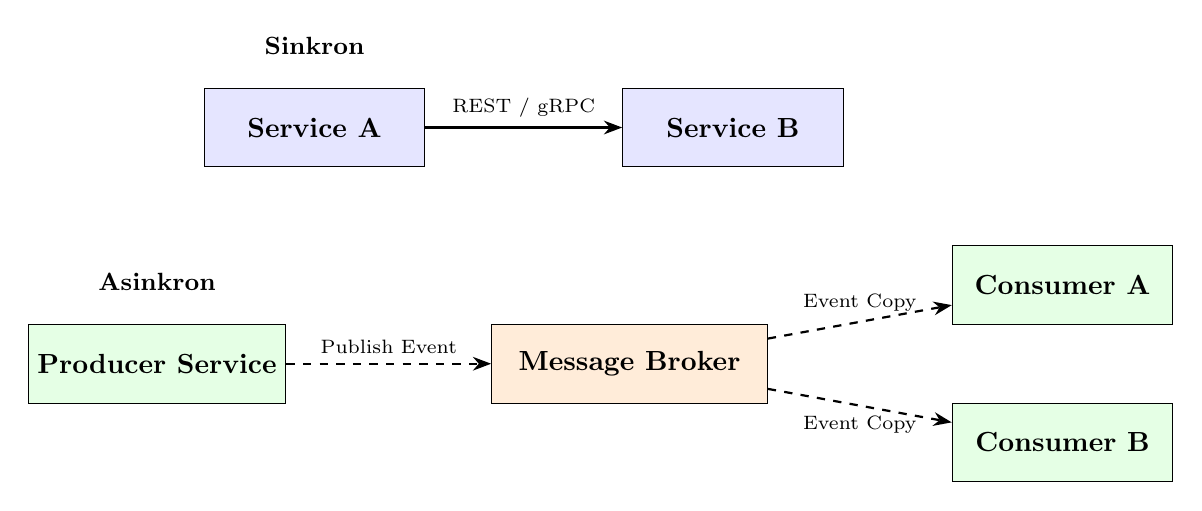
\begin{tikzpicture}[
		component/.style={draw, fill=blue!10, minimum width=2.8cm, minimum height=1cm, font=\bfseries, align=center},
		service/.style={draw, fill=green!10, minimum width=2.8cm, minimum height=1cm, font=\bfseries, align=center},
		broker/.style={draw, fill=orange!15, minimum width=3.5cm, minimum height=1cm, font=\bfseries, align=center},
		conn/.style={->, thick, >=Stealth},
		async/.style={->, thick, dashed, >=Stealth},
		label/.style={font=\scriptsize},
		node distance=1.4cm and 2.5cm
		]
		% Sinkron - REST/gRPC
		\node[component] (client1) at (0,0) {Service A};
		\node[component, right=of client1] (service1) {Service B};
		
		\draw[conn] (client1) -- node[above, label] {REST / gRPC} (service1);
		
		% Label
		\node[font=\small, above=0.3cm of client1, align=center] {\textbf{Sinkron}};
		
		% Asinkron - Event-driven
		\node[service] (producer) at (-2,-3) {Producer Service};
		\node[broker] (broker) at (4,-3) {Message Broker};
		\node[service] (consumer1) at (9.5,-2) {Consumer A};
		\node[service] (consumer2) at (9.5,-4) {Consumer B};
		
		\draw[async] (producer) -- node[above, label] {Publish Event} (broker);
		\draw[async] (broker) -- node[above, label] {Event Copy} (consumer1);
		\draw[async] (broker) -- node[below, label] {Event Copy} (consumer2);
		 
		% Label
		\node[font=\small, above=0.3cm of producer, align=center] {\textbf{Asinkron}};
		
	\end{tikzpicture}
\end{figure}

\subsection{Komunikasi Sinkron: REST dan gRPC}

Komunikasi sinkron adalah pola komunikasi di mana satu layanan mengirim permintaan dan menunggu respons dari layanan lain secara langsung sebelum melanjutkan proses eksekusi. Pendekatan ini mudah dipahami dan diimplementasikan karena mirip dengan cara kerja pemanggilan fungsi pada sistem terpusat. Dua teknologi utama yang digunakan dalam komunikasi sinkron adalah REST dan gRPC.

REST (Representational State Transfer) merupakan protokol komunikasi berbasis HTTP yang telah menjadi standar de facto dalam pengembangan API. REST menggunakan metode HTTP seperti GET, POST, PUT, dan DELETE untuk mengelola sumber daya, serta mendukung format pertukaran data seperti JSON atau XML. Keunggulan REST terletak pada kesederhanaannya, kompatibilitas luas, dan kemudahan dalam integrasi lintas platform. REST juga memiliki ekosistem alat pendukung yang luas, termasuk dokumentasi otomatis (seperti Swagger/OpenAPI), testing, dan monitoring. Namun, karena menggunakan HTTP/1.1, REST memiliki keterbatasan dalam hal performa untuk kebutuhan sistem real-time atau komunikasi intensif.

gRPC (gRPC Remote Procedure Call) adalah teknologi komunikasi modern yang dikembangkan oleh Google dan dirancang untuk mengatasi keterbatasan REST dalam konteks performa dan efisiensi. gRPC menggunakan HTTP/2 sebagai protokol transport dan Protocol Buffers (protobuf) sebagai format serialisasi data yang ringan dan cepat. Pendekatan ini memungkinkan layanan untuk berkomunikasi melalui pemanggilan metode secara langsung seolah-olah berada dalam satu sistem, meskipun sebenarnya tersebar di jaringan. gRPC mendukung komunikasi dua arah (bidirectional streaming), multiplexing, dan efisiensi bandwidth yang lebih baik dibandingkan REST. Teknologi ini sangat cocok untuk komunikasi antar layanan dengan latency rendah, komunikasi streaming, atau kebutuhan real-time seperti pada sistem IoT, machine learning inference, atau gaming backend.

Meski komunikasi sinkron memiliki banyak manfaat, penggunaannya perlu dipertimbangkan secara hati-hati dalam konteks mikroservis. Ketergantungan antar layanan secara sinkron dapat menimbulkan efek domino saat salah satu layanan gagal merespons, dan hal ini bisa mengganggu keseluruhan sistem. Oleh karena itu, penerapan pola seperti circuit breaker, timeout, dan retry menjadi penting untuk meningkatkan resiliensi sistem sinkron.

Dalam praktiknya, REST sering digunakan untuk integrasi yang bersifat publik atau antar tim karena lebih human-readable dan lebih mudah di-debug. Sementara itu, gRPC lebih umum digunakan dalam komunikasi internal antarlayanan karena efisiensi dan performanya yang tinggi. Pemilihan antara REST dan gRPC perlu disesuaikan dengan kebutuhan domain, latensi yang diharapkan, serta tingkat kontrol terhadap skema data.

\subsection{Komunikasi Asinkron: Event-Driven Messaging}

Komunikasi asinkron dalam arsitektur mikroservis adalah pendekatan di mana layanan pengirim tidak menunggu respons langsung dari layanan penerima. Sebagai gantinya, pengirim hanya mengirimkan pesan atau event ke sistem perantara (seperti message broker), dan proses eksekusi dapat langsung dilanjutkan tanpa tergantung pada status layanan penerima. Pola ini banyak digunakan dalam sistem yang membutuhkan skalabilitas tinggi, toleransi terhadap kegagalan, dan pemrosesan yang terdistribusi.

Pendekatan event-driven messaging menjadikan event sebagai satuan komunikasi utama antara layanan. Event merepresentasikan suatu kejadian yang terjadi dalam sistem, seperti “OrderCreated”, “PaymentConfirmed”, atau “StockDepleted”. Layanan yang menghasilkan event disebut sebagai *event producer*, sedangkan layanan yang tertarik terhadap event tertentu disebut sebagai *event consumer*. Event disalurkan melalui *event bus* atau *message broker* seperti Apache Kafka, RabbitMQ, Amazon SNS/SQS, atau NATS.

Keuntungan utama dari komunikasi asinkron adalah peningkatan fleksibilitas dan loose coupling. Layanan tidak perlu mengetahui siapa konsumen dari event yang mereka hasilkan, sehingga setiap layanan dapat berkembang dan berubah secara independen tanpa memengaruhi layanan lain. Selain itu, komunikasi asinkron memungkinkan pemrosesan paralel dan non-blocking, yang ideal untuk skenario beban tinggi atau sistem yang terus-menerus menerima input dari berbagai sumber secara real-time.

Mekanisme publish/subscribe menjadi dasar umum dalam implementasi komunikasi asinkron. Dalam pola ini, satu atau lebih layanan dapat menerbitkan event ke topik tertentu, dan semua layanan yang berlangganan ke topik tersebut akan menerima salinan event tersebut. Hal ini memfasilitasi integrasi multi-layanan tanpa membuat ketergantungan eksplisit antar layanan. Selain publish/subscribe, ada juga pola message queue, di mana pesan dikonsumsi satu per satu oleh layanan penerima yang mengantre, seperti dalam kasus job worker atau pemrosesan batch.

Meskipun komunikasi asinkron memberikan banyak manfaat, ada sejumlah tantangan yang perlu diperhatikan. Salah satunya adalah kompleksitas dalam pelacakan alur data (observability), karena event tidak mengalir secara linier seperti dalam komunikasi sinkron. Selain itu, aspek seperti konsistensi data terdistribusi, pengelolaan retry dan duplikasi, serta idempotensi operasi menjadi hal yang penting untuk dipertimbangkan agar sistem tetap andal dan dapat di-debug dengan baik.

Dalam arsitektur mikroservis skala besar, komunikasi asinkron sering digunakan ber\-samaan dengan komunikasi sinkron. Kombinasi keduanya memungkinkan arsitektur yang adaptif, efisien, dan tangguh dalam menghadapi berbagai beban dan kondisi operasional.

\subsection{Perbandingan dan Trade-Off}

Pemilihan antara komunikasi sinkron dan asinkron dalam arsitektur mikroservis bukanlah keputusan yang bersifat mutlak, melainkan bergantung pada konteks bisnis, kebutuhan teknis, dan karakteristik beban kerja. Masing-masing pendekatan memiliki keunggulan dan kelemahan yang harus dipertimbangkan secara matang agar integrasi antar layanan tetap efisien, andal, dan sesuai dengan ekspektasi sistem.

Komunikasi \textbf{sinkron}, seperti REST atau gRPC, menawarkan model yang sederhana dan mudah dipahami. Layanan pengirim akan langsung mendapatkan hasil dari permintaan yang dikirimkan, sehingga cocok untuk skenario yang membutuhkan respons segera, validasi input, atau proses yang sifatnya interaktif. Keunggulan komunikasi sinkron terletak pada kesederhanaan implementasi dan kemudahan debugging karena alur eksekusi bersifat deterministik dan linier. Namun, pendekatan ini menimbulkan \textit{tight coupling} antar layanan dan meningkatkan risiko kegagalan berantai (cascading failure) jika salah satu layanan tidak responsif. Ketergantungan pada waktu respons juga membuat sistem lebih sulit diskalakan secara elastis.

Di sisi lain, komunikasi \textbf{asinkron} seperti event-driven messaging menawarkan fleksibilitas yang tinggi dan mendukung \textit{loose coupling} antar layanan. Layanan pengirim tidak perlu mengetahui keberadaan atau status penerima, sehingga setiap layanan dapat berkembang secara independen. Komunikasi asinkron juga memfasilitasi pemrosesan paralel dan batch, menjadikannya pilihan ideal untuk sistem berskala besar dengan beban tidak terduga. Namun, pendekatan ini menambah kompleksitas dalam hal observabilitas, debugging, dan manajemen konsistensi data. Tanpa strategi seperti event replay, idempotensi, dan monitoring yang baik, komunikasi asinkron dapat menyulitkan pemeliharaan sistem secara keseluruhan.

Dalam praktiknya, banyak sistem mikroservis modern menggabungkan kedua pendekatan ini. Komunikasi sinkron digunakan untuk operasi yang membutuhkan kejelasan alur dan hasil langsung, sementara komunikasi asinkron digunakan untuk pemrosesan latar belakang, integrasi lintas layanan, atau notifikasi yang tidak membutuhkan tanggapan segera. Trade-off antara keduanya mencakup aspek performa, skalabilitas, kompleksitas, dan keandalan. Tabel \ref{tab:komunikasi-sinkron-vs-asinkron} merangkum perbandingan antara komunikasi sinkron dan asinkron dalam berbagai aspek penting.

\begin{table}[h]
	\centering
	\caption{Perbandingan Komunikasi Sinkron dan Asinkron}
	\label{tab:komunikasi-sinkron-vs-asinkron}
	\begin{tabular}{|p{.18\textwidth}|p{.36\textwidth}|p{.36\textwidth}|}
		\hline
		\textbf{Aspek} & \textbf{Sinkron (REST/gRPC)} & \textbf{Asinkron (Messaging)} \\
		\hline
		Model Komunikasi & Request/Response langsung & Event-based, tidak menunggu respons \\
		\hline
		Keterkaitan Layanan & Tight coupling & Loose coupling \\
		\hline
		Ketergantungan Respons & Ya, harus tersedia saat itu juga & Tidak, bisa diproses nanti \\
		\hline
		Skalabilitas & Terbatas oleh layanan terlemah & Tinggi, mendukung pemrosesan paralel \\
		\hline
		Kompleksitas Debugging & Rendah, alur linier & Tinggi, alur tidak deterministik \\
		\hline
		Kesesuaian Penggunaan & Validasi langsung, interaksi user & Proses latar belakang, integrasi layanan \\
		\hline
	\end{tabular}
\end{table}

Dengan memahami karakteristik dan trade-off dari masing-masing pendekatan, arsitek sistem dapat merancang pola komunikasi yang paling sesuai dengan kebutuhan bisnis dan teknis. Pendekatan yang adaptif dan hibrid sering kali menjadi solusi terbaik dalam implementasi mikroservis skala besar.




\section{Komponen Infrastruktur Mikroservis}

Dalam arsitektur mikroservis, keberhasilan implementasi tidak hanya bergantung pada desain layanan, tetapi juga pada infrastruktur pendukung yang memastikan komunikasi, konfigurasi, keamanan, dan orkestrasi layanan berjalan dengan lancar. Komponen-komponen infrastruktur berikut memainkan peran penting dalam menjaga performa dan stabilitas sistem mikroservis secara keseluruhan.

\subsection{API Gateway}

API Gateway merupakan titik masuk tunggal (single entry point) untuk semua permintaan yang masuk ke sistem mikroservis. Komponen ini bertugas menerima permintaan dari klien eksternal dan meneruskannya ke layanan internal yang sesuai. Selain routing permintaan, API Gateway juga dapat menangani berbagai tanggung jawab lintas layanan seperti autentikasi, otorisasi, rate limiting, caching, logging, dan transformasi data (misalnya dari format JSON ke XML).

Dengan menggunakan API Gateway, arsitektur mikroservis menjadi lebih aman dan terkontrol, karena layanan backend tidak langsung terekspos ke publik. Hal ini juga menyederhanakan integrasi klien karena klien cukup berinteraksi dengan satu endpoint, tanpa perlu mengetahui lokasi atau struktur masing-masing layanan. Contoh populer API Gateway meliputi Kong, NGINX, Apigee, dan Spring Cloud Gateway.

\subsection{Service Registry \& Discovery}

Dalam lingkungan mikroservis yang dinamis, di mana layanan dapat di-deploy, dipindahkan, atau dihentikan secara otomatis, diperlukan mekanisme untuk menemukan lokasi layanan yang aktif secara real-time. Service Registry adalah komponen yang menyimpan informasi tentang semua instance layanan yang berjalan, termasuk alamat IP, port, dan metadata terkait.

Service Discovery memungkinkan layanan lain untuk menemukan dan berkomunikasi dengan layanan tersebut berdasarkan nama logis, bukan alamat fisik yang statis. Ada dua pendekatan utama: \textit{client-side discovery}, di mana klien langsung mengambil data dari service registry, dan \textit{server-side discovery}, di mana komponen perantara (seperti load balancer atau API gateway) menangani proses pencarian. Contoh alat untuk service registry dan discovery termasuk Eureka (Spring Cloud), Consul, dan Zookeeper.

\subsection{Configuration Server}

Configuration Server berfungsi untuk menyediakan konfigurasi eksternal secara terpusat bagi seluruh layanan mikroservis. Dalam arsitektur mikroservis, sangat tidak efisien dan rentan kesalahan jika setiap layanan menyimpan konfigurasinya secara lokal. Dengan Configuration Server, konfigurasi dapat dikelola, diperbarui, dan diterapkan secara konsisten tanpa perlu melakukan ulang build dan redeploy layanan.

Server konfigurasi biasanya terhubung dengan repositori git atau sumber lainnya, dan setiap layanan dapat mengambil konfigurasi berdasarkan nama aplikasi, profil lingkungan (development, staging, production), dan versi tertentu. Selain mendukung manajemen konfigurasi terpusat, komponen ini juga mempermudah audit dan rollback perubahan. Salah satu implementasi yang populer adalah Spring Cloud Config Server.

\subsection{Service Mesh (Opsional)}

Service Mesh adalah lapisan infrastruktur opsional yang mengelola komunikasi antar layanan mikroservis tanpa harus mengubah kode aplikasi. Service mesh menyediakan fitur-fitur seperti observabilitas, keamanan, enkripsi, load balancing, retry, dan circuit breaking secara terpusat melalui sidecar proxy yang berjalan berdampingan dengan setiap layanan (biasanya menggunakan Envoy atau Linkerd).

Dengan service mesh, pengembang dapat memisahkan logika komunikasi dari logika bisnis layanan. Ini sangat membantu dalam sistem berskala besar yang terdiri dari ratusan atau ribuan layanan. Service mesh juga menyediakan dashboard monitoring dan tracing yang komprehensif, mendukung TLS antar layanan, serta mempermudah deployment canary atau blue/green. Contoh implementasi populer termasuk Istio, Linkerd, dan Kuma.

Meskipun membawa banyak manfaat, penerapan service mesh juga menambah kompleksitas dan beban operasional, sehingga disarankan hanya digunakan pada tahap skala lanjut ketika sistem telah cukup besar dan membutuhkan kontrol komunikasi yang lebih canggih. Gambar~\ref{fig:infra-microservices} menggambarkan komponen infrastruktur utama dalam arsitektur mikroservis, termasuk API Gateway, Service Registry, Configuration Server, dan Sidecar Proxy yang menyertai layanan.

\begin{figure}[h]
	\centering
	\caption{Komponen Infrastruktur dalam Arsitektur Mikroservis}
	\vspace{0.5em}
	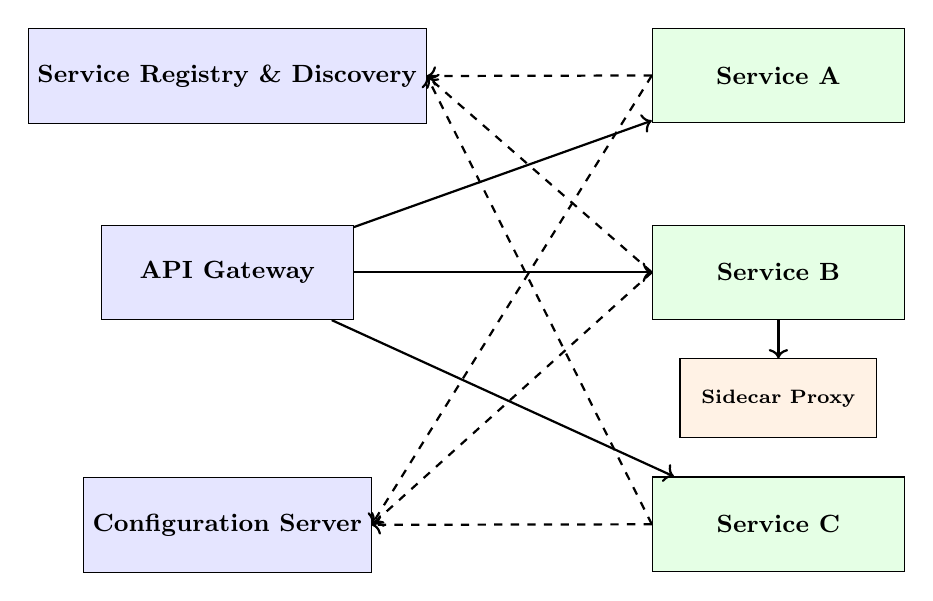
\begin{tikzpicture}[
		component/.style={draw, fill=blue!10, minimum width=3.2cm, minimum height=1.2cm, font=\small\bfseries, align=center},
		service/.style={draw, fill=green!10, minimum width=3.2cm, minimum height=1.2cm, font=\small\bfseries, align=center},
		sidecar/.style={draw, fill=orange!10, minimum width=2.5cm, minimum height=1.0cm, font=\scriptsize\bfseries, align=center},
		conn/.style={->, thick},
		dashedconn/.style={->, thick, dashed},
		node distance=1.4cm
		]
		
		% Left-side components
		\node[component] (gateway) at (0, 0) {API Gateway};
		\node[component, below=of gateway] (registry) at (0, 4.5) {Service Registry \& Discovery};
		\node[component, below=of registry] (config) at (0, -1.2) {Configuration Server};
		
		% Right-side services
		\node[service] (svc1) at (7, 2.5) {Service A};
		\node[service] (svc2) at (7, 0) {Service B};
		\node[sidecar] (sidecar) at (7, -1.6) {Sidecar Proxy};
		\node[service] (svc3) at (7, -3.2) {Service C};
		
		% Connections
		\draw[conn] (gateway) -- (svc1);
		\draw[conn] (gateway) -- (svc2);
		\draw[conn] (gateway) -- (svc3);
		\draw[conn] (svc2) -- (sidecar);
		
		% Dashed lines for infra dependencies
		\draw[dashedconn] (svc1.west) -- (registry.east);
		\draw[dashedconn] (svc2.west) -- (registry.east);
		\draw[dashedconn] (svc3.west) -- (registry.east);
		
		\draw[dashedconn] (svc1.west) -- (config.east);
		\draw[dashedconn] (svc2.west) -- (config.east);
		\draw[dashedconn] (svc3.west) -- (config.east);
		
	\end{tikzpicture}
	\label{fig:infra-microservices}
\end{figure}




\section{Pola Implementasi Mikroservis}

Penerapan arsitektur mikroservis yang efektif tidak hanya bergantung pada pemecahan sistem menjadi layanan-layanan kecil, tetapi juga pada pola-pola implementasi yang mendukung modularitas, keandalan, dan skalabilitas sistem. Pola-pola berikut merupakan pendekatan umum yang digunakan untuk membangun dan mengelola sistem mikroservis dengan baik.



\subsection{Decomposition by Business Capability}

Pola ini menekankan pemisahan layanan berdasarkan kapabilitas bisnis, bukan berdasarkan lapisan teknis. Setiap layanan bertanggung jawab atas satu domain atau fungsi bisnis tertentu yang utuh dan bermakna secara operasional. Misalnya, dalam sistem e-commerce, layanan dapat dipisah menjadi “Order Service”, “Payment Service”, dan “Inventory Service”.

Pendekatan ini mendorong penerapan prinsip bounded context dari domain-driven design (DDD), di mana masing-masing layanan memiliki model data, logika bisnis, dan kontrak API yang spesifik terhadap domainnya. Hasilnya adalah struktur sistem yang lebih modular, mudah dikembangkan oleh tim yang terdistribusi, dan relevan terhadap kebutuhan pengguna akhir. Lihat Gambar \ref{fig:decomposition-by-capability} untuk ilustrasinya.

\begin{figure}[h]
	\centering
	\caption{Decomposition by Business Capability dalam Mikroservis}
	\vspace{0.5em}
	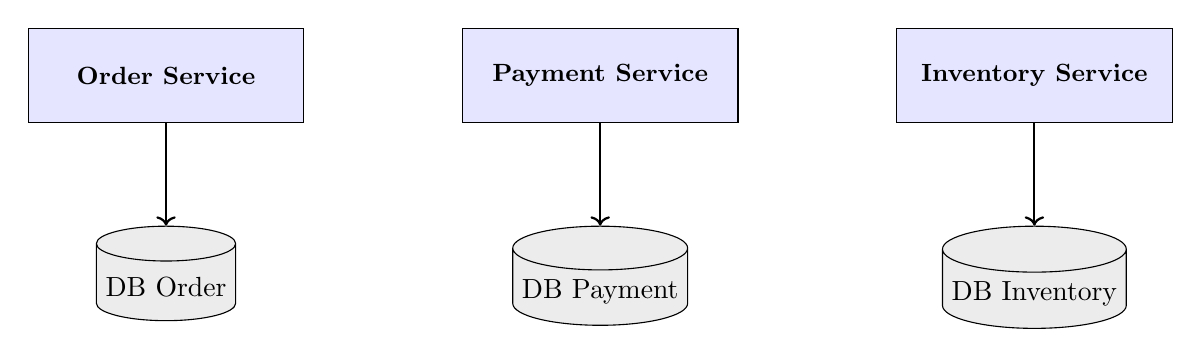
\begin{tikzpicture}[
		service/.style={draw, fill=blue!10, minimum width=3.5cm, minimum height=1.2cm, font=\small\bfseries, align=center},
		db/.style={draw, cylinder, shape border rotate=90, aspect=0.25, minimum height=1.2cm, minimum width=1.2cm, fill=gray!15},
		conn/.style={->, thick},
		label/.style={font=\scriptsize},
		node distance=1.3cm and 2cm
		]
		
		% Layanan-layanan
		\node[service] (order) {Order Service};
		\node[service, right=of order] (payment) {Payment Service};
		\node[service, right=of payment] (inventory) {Inventory Service};
		
		% Database masing-masing
		\node[db, below=of order] (db1) {DB Order};
		\node[db, below=of payment] (db2) {DB Payment};
		\node[db, below=of inventory] (db3) {DB Inventory};
		
		% Connections
		\draw[conn] (order) -- (db1);
		\draw[conn] (payment) -- (db2);
		\draw[conn] (inventory) -- (db3);
		
	\end{tikzpicture}
	\label{fig:decomposition-by-capability}
\end{figure}


\subsection{Database per Service}

Dalam arsitektur mikroservis, disarankan agar setiap layanan memiliki database-nya sendiri yang tidak langsung diakses oleh layanan lain. Pola ini dikenal sebagai \textit{Database per Service}. Tujuannya adalah untuk memastikan isolasi data, menghindari tight coupling pada level penyimpanan, dan memungkinkan pengambilan keputusan teknologi yang berbeda untuk masing-masing layanan (polyglot persistence).

Penerapan pola ini juga meningkatkan kebebasan layanan dalam mengatur skema data, optimasi query, serta melakukan migrasi data tanpa memengaruhi layanan lain. Namun, pola ini menimbulkan tantangan dalam menjaga konsistensi data global. Oleh karena itu, strategi seperti event-driven architecture, event sourcing, atau saga pattern sering digunakan sebagai pelengkap untuk memastikan integritas antar layanan. Gambar~\ref{fig:database-per-service} menunjukkan bahwa setiap layanan dalam arsitektur mikroservis memiliki database tersendiri untuk menjaga isolasi data dan otonomi layanan.

\begin{figure}[h]
	\centering
	\caption{Setiap layanan dalam arsitektur mikroservis memiliki database tersendiri untuk menjaga isolasi data dan otonomi layanan.}
	\vspace{0.5em}
	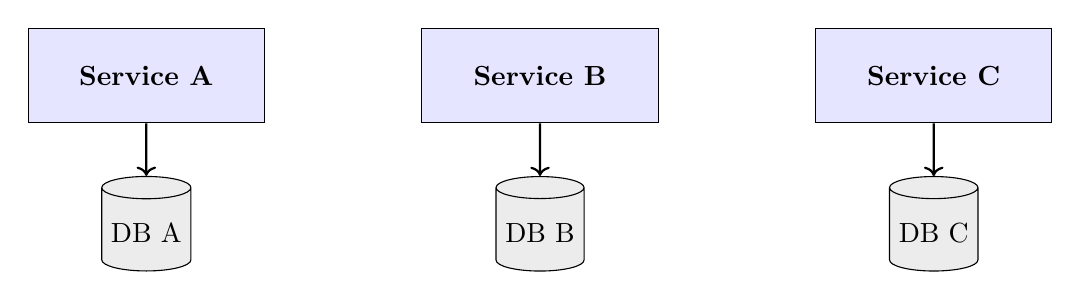
\begin{tikzpicture}[
		service/.style={draw, fill=blue!10, minimum width=3cm, minimum height=1.2cm, font=\bfseries},
		db/.style={draw, cylinder, shape border rotate=90, aspect=0.25, minimum height=1.2cm, minimum width=1cm, fill=gray!15},
		conn/.style={->, thick}
		]
		% Services
		\node[service] (svc1) at (0,0) {Service A};
		\node[service] (svc2) at (5,0) {Service B};
		\node[service] (svc3) at (10,0) {Service C};
		
		% Databases
		\node[db] (db1) at (0,-2) {DB A};
		\node[db] (db2) at (5,-2) {DB B};
		\node[db] (db3) at (10,-2) {DB C};
		
		% Connections
		\draw[conn] (svc1) -- (db1);
		\draw[conn] (svc2) -- (db2);
		\draw[conn] (svc3) -- (db3);
		
	\end{tikzpicture}
	\label{fig:database-per-service}
\end{figure}


\subsection{Circuit Breaker Pattern}

Circuit Breaker Pattern merupakan pola yang digunakan untuk meningkatkan ketahanan sistem terhadap kegagalan, terutama pada komunikasi antar layanan. Pola ini bekerja mirip dengan saklar listrik: jika layanan target gagal merespons atau mengalami kesalahan berulang, circuit breaker akan “terbuka” dan memutus aliran permintaan selama periode tertentu. Hal ini mencegah sistem terus-menerus mengirim permintaan ke layanan yang bermasalah dan menghindari efek cascading failure.

Circuit breaker memiliki tiga kondisi utama: \textit{Closed}, \textit{Open}, dan \textit{Half-Open}. Dalam keadaan \textbf{Closed}, permintaan diteruskan seperti biasa ke layanan target. Ketika terjadi kegagalan berulang, status berubah menjadi \textbf{Open} dan permintaan langsung ditolak atau diarahkan ke fallback mechanism. Setelah waktu tertentu, circuit breaker masuk ke status \textbf{Half-Open} untuk mengizinkan beberapa permintaan percobaan. Jika layanan pulih, circuit breaker kembali ke \textbf{Closed}; jika tidak, tetap berada dalam kondisi \textbf{Open}. Framework seperti Resilience4j dan Hystrix mendukung implementasi pola ini.


Pola ini sangat penting dalam mencegah cascading failure dan mempertahankan stabilitas sistem secara keseluruhan. Banyak framework seperti Resilience4j dan Hystrix menyediakan dukungan bawaan untuk pola ini. Gambar~\ref{fig:circuit-breaker-pattern} menggambarkan cara kerja circuit breaker yang memutus komunikasi sementara ke layanan target saat terjadi kegagalan berulang untuk mencegah gangguan menyebar.

\begin{figure}[h]
	\centering
	\caption{Ilustrasi Circuit Breaker Pattern untuk mencegah komunikasi berulang ke layanan yang gagal}
	\vspace{0.5em}
	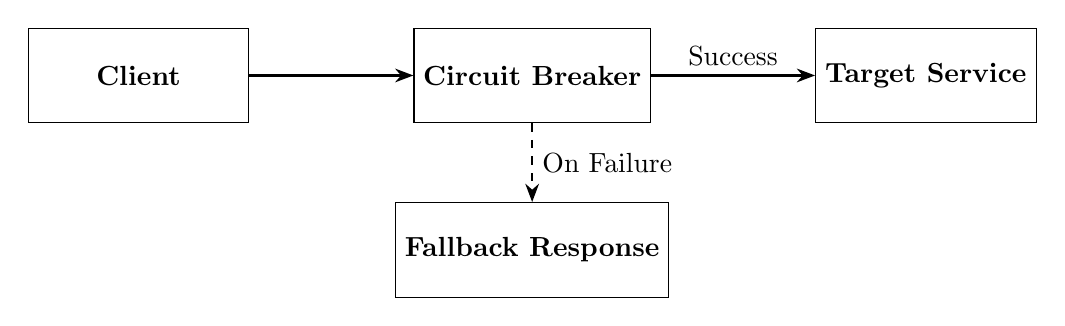
\begin{tikzpicture}[
		component/.style={draw, minimum width=2.8cm, minimum height=1.2cm, font=\bfseries, align=center},
		state/.style={draw, ellipse, minimum width=2.5cm, minimum height=1.2cm, fill=gray!15},
		conn/.style={->, thick},
		alt/.style={dashed, thick, ->},
		>=Stealth
		]
		
		% Nodes
		\node[component] (client) at (0, 0) {Client};
		\node[component] (cb) at (5, 0) {Circuit Breaker};
		\node[component] (service) at (10, 0) {Target Service};
		\node[component, below=1cm of cb] (fallback) {Fallback Response};
		
		% Connections
		\draw[conn] (client) -- (cb);
		\draw[conn] (cb) -- node[above]{Success} (service);
		\draw[alt] (cb) -- node[right]{On Failure} (fallback);
		
	\end{tikzpicture}
	\label{fig:circuit-breaker-pattern}
\end{figure}

\subsection{Saga Pattern}

Saga Pattern digunakan untuk mengelola transaksi terdistribusi antar beberapa layanan mikroservis. Karena transaksi ACID tidak dapat dilakukan secara lintas layanan yang memiliki database terpisah, saga pattern menawarkan alternatif berbasis rangkaian event atau command yang terkoordinasi.

Dalam saga pattern, proses bisnis yang melibatkan beberapa layanan dibagi menjadi serangkaian transaksi lokal. Setiap transaksi lokal dilakukan oleh satu layanan dan diikuti oleh event atau command yang memicu transaksi berikutnya. Jika terjadi kegagalan di tengah proses, layanan akan mengeksekusi aksi kompensasi untuk membatalkan efek dari transaksi sebelumnya (compensating transaction).

Ada dua pendekatan utama dalam saga pattern: \textit{choreography}, di mana layanan saling merespons event tanpa koordinasi pusat, dan \textit{orchestration}, di mana ada satu layanan koordinator yang mengatur urutan dan pengambilan keputusan. Saga sangat berguna untuk menjaga integritas data dalam sistem terdistribusi tanpa bergantung pada transaksi global. Gambar~\ref{fig:saga-pattern-orchestration} menunjukkan implementasi Saga Pattern dengan pendekatan orchestration, di mana koordinasi antar transaksi lokal dilakukan oleh layanan orkestra untuk menjaga integritas proses bisnis terdistribusi.

\begin{figure}[h]
	\centering
	\caption{Saga Pattern (Orchestration): Koordinasi transaksi lokal oleh layanan orkestra}
	\vspace{0.5em}
	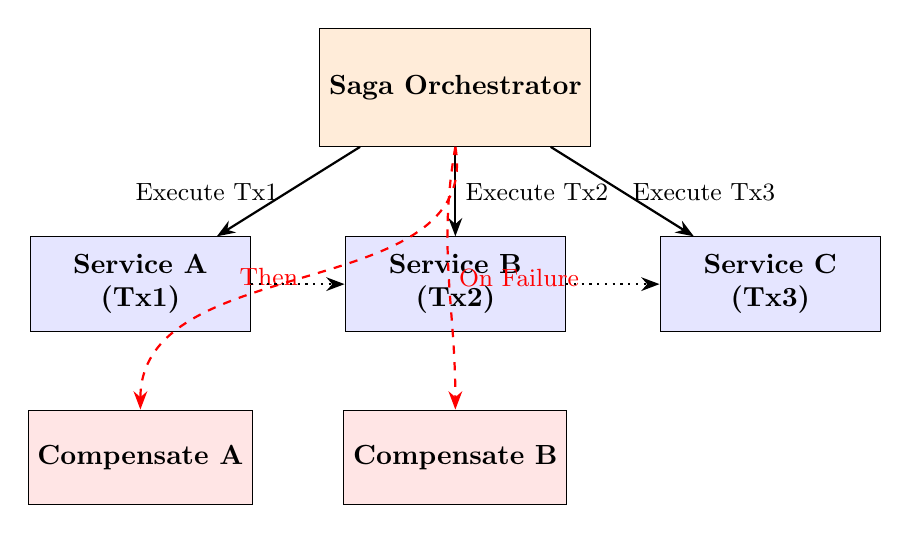
\begin{tikzpicture}[
		service/.style={draw, minimum width=2.8cm, minimum height=1.2cm, font=\bfseries, align=center, fill=blue!10},
		orchestrator/.style={draw, minimum width=3cm, minimum height=1.5cm, font=\bfseries, align=center, fill=orange!15},
		conn/.style={->, thick, >=Stealth},
		rollback/.style={->, thick, dashed, red, >=Stealth},
		flow/.style={->, thick, dotted, >=Stealth}
		]
		
		% Nodes
		\node[orchestrator] (orchestrator) at (0, 2.5) {Saga Orchestrator};
		
		\node[service] (service1) at (-4, 0) {Service A \\ (Tx1)};
		\node[service] (service2) at (0, 0) {Service B \\ (Tx2)};
		\node[service] (service3) at (4, 0) {Service C \\ (Tx3)};
		
		% Compensation handlers
		\node[service, fill=red!10] (comp1) at (-4, -2.2) {Compensate A};
		\node[service, fill=red!10] (comp2) at (0, -2.2) {Compensate B};
		
		% Connections from orchestrator to services
		\draw[conn] (orchestrator) -- node[left, font=\small] {Execute Tx1} (service1);
		\draw[conn] (orchestrator) -- node[right, font=\small] {Execute Tx2} (service2);
		\draw[conn] (orchestrator) -- node[right, font=\small] {Execute Tx3} (service3);
		
		% Compensation arrows (rollback)
		\draw[rollback] (orchestrator.south) to[out=-100,in=90] node[right, font=\small] {On Failure} (comp2.north);
		\draw[rollback] (orchestrator.south) to[out=-80,in=90] node[left, font=\small] {Then} (comp1.north);
		
		% Logical dotted flow
		\draw[flow] (service1) -- (service2);
		\draw[flow] (service2) -- (service3);
		
	\end{tikzpicture}
	\label{fig:saga-pattern-orchestration}
\end{figure}




\subsection{Sidecar Pattern}

Sidecar Pattern adalah pendekatan di mana komponen tambahan ditempatkan berdampingan dengan layanan utama dalam satu unit deploy (biasanya satu pod dalam Kubernetes). Komponen ini menjalankan fungsi tambahan seperti logging, observability, pengelolaan konfigurasi, atau komunikasi jaringan, tanpa menambah kompleksitas ke dalam kode layanan utama.

Sidecar bekerja secara terpisah, namun saling melengkapi dengan layanan utama. Contoh paling umum adalah sidecar proxy seperti Envoy dalam arsitektur service mesh. Sidecar dapat menyederhanakan pengembangan layanan karena berbagai fungsi infrastruktur dan cross-cutting concerns dapat didelegasikan ke sidecar tanpa perlu ditanamkan langsung ke dalam kode aplikasi.

Pola ini juga mendukung fleksibilitas operasional, karena sidecar dapat diperbarui, dikonfigurasi ulang, atau dikelola secara terpisah dari layanan utama. Meskipun menambah konsumsi sumber daya, sidecar pattern memberikan cara modular untuk memperkaya layanan dengan kapabilitas tambahan secara terisolasi. Gambar~\ref{fig:sidecar-pattern} menggambarkan pola Sidecar, di mana layanan utama dan sidecar container berjalan berdampingan dalam satu unit deploy untuk memisahkan fungsi utama dan infrastruktur.

\begin{figure}[h]
	\centering
	\caption{Sidecar Pattern: Layanan utama dan sidecar berjalan berdampingan dalam satu unit deploy}
	\vspace{0.5em}
	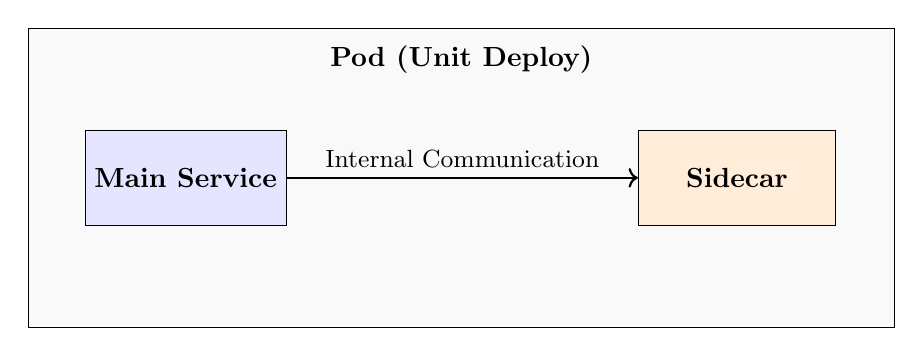
\begin{tikzpicture}[
		box/.style={draw, minimum height=3.8cm, minimum width=11cm, fill=gray!5},
		service/.style={draw, fill=blue!10, minimum width=2.5cm, minimum height=1.2cm, font=\bfseries, align=center},
		sidecar/.style={draw, fill=orange!15, minimum width=2.5cm, minimum height=1.2cm, font=\bfseries, align=center},
		label/.style={font=\small\bfseries}
		]
		
		% Pod box with label above
		\node[box] (pod) {};
		\node[font=\bfseries, above=-.7cm of pod.north] {Pod (Unit Deploy)};
		
		% Inside Pod: Main Service and Sidecar
		\node[service] (main) at (-3.5, 0) {Main Service};
		\node[sidecar] (sc) at (3.5, 0) {Sidecar};
		
		% Internal arrow
		\draw[->, thick] (main) -- node[above, font=\small] {Internal Communication} (sc);
		
	\end{tikzpicture}
	\label{fig:sidecar-pattern}
\end{figure}


\section{Teknologi Pendukung}

Keberhasilan implementasi arsitektur mikroservis tidak hanya bergantung pada desain dan pola, tetapi juga pada pemilihan teknologi pendukung yang tepat. Teknologi-teknologi ini membantu dalam aspek containerisasi, orkestrasi, pengembangan layanan, monitoring, serta pengelolaan komunikasi antar layanan. Berikut adalah teknologi-teknologi utama yang umum digunakan dalam lingkungan mikroservis.

\subsection{Docker dan Kubernetes}

\textbf{Docker} merupakan teknologi containerisasi yang memungkinkan pengemasan aplikasi dan seluruh dependensinya ke dalam satu unit yang dapat dijalankan secara konsisten di berbagai lingkungan. Dalam konteks mikroservis, Docker memungkinkan setiap layanan dibangun dan dijalankan sebagai container yang terisolasi, sehingga mempermudah proses deployment, testing, dan scaling.

\textbf{Kubernetes}, di sisi lain, adalah platform orkestrasi container yang dirancang untuk mengelola container dalam skala besar. Kubernetes menyediakan fitur seperti penjadwalan pod, auto-scaling, rolling update, service discovery, dan manajemen konfigurasi. Dalam sistem mikroservis, Kubernetes memegang peran penting dalam mengatur lifecycle dan komunikasi antar layanan containerized, serta menyediakan abstraksi infrastruktur yang powerful dan resilient.

Kombinasi Docker dan Kubernetes telah menjadi standar de facto dalam implementasi mikroservis modern karena fleksibilitas dan skalabilitas yang ditawarkannya.

\subsection{Framework untuk Pengembangan Mikroservis}

Berbagai bahasa pemrograman dan ekosistem menyediakan framework yang dirancang khusus untuk mendukung pengembangan layanan mikroservis. Framework ini umumnya menyediakan dukungan untuk pembuatan REST API, dependency injection, konfigurasi terpusat, integrasi dengan message broker, serta kemudahan integrasi dengan sistem observabilitas dan deployment container-based.

Beberapa contoh populer meliputi:

\begin{itemize}
	\item \textbf{Spring Boot} (Java/Kotlin): Framework yang menyediakan pendekatan konvensi-di-atas-konfigurasi dan dukungan penuh terhadap ekosistem Spring Cloud untuk membangun layanan mikroservis skala besar.
	
	\item \textbf{Micronaut} (Java/Kotlin/Groovy): Framework ringan dengan startup time cepat, mendukung native image via GraalVM dan dependency injection waktu kompilasi, cocok untuk aplikasi cloud-native dan serverless.
	
	\item \textbf{Express.js} (Node.js): Framework minimalis dan fleksibel yang banyak digunakan untuk membangun layanan RESTful, dengan ekosistem middleware yang luas.
	
	\item \textbf{FastAPI} (Python): Framework modern berbasis Python yang mendukung asynchronous programming, validasi input otomatis, dan dokumentasi API otomatis berbasis OpenAPI.
	
	\item \textbf{Go Kit} (Go): Toolkit untuk membangun layanan mikroservis di Go dengan fokus pada modularitas, logging, service discovery, dan transport abstraction.
	
	\item \textbf{ASP.NET Core} (C\#): Framework open-source dari Microsoft untuk membangun layanan web modern, termasuk dukungan penuh untuk REST API, gRPC, dan integrasi dengan Azure.
\end{itemize}

Pemilihan framework bergantung pada kebutuhan domain, keahlian tim, dan integrasi dengan platform yang digunakan. Yang terpenting, framework tersebut harus mendukung prinsip desain mikroservis seperti independensi layanan, skalabilitas, dan observabilitas.


\subsection{Observability Tools: Prometheus, Grafana}

\textbf{Observability} adalah elemen kunci dalam sistem mikroservis karena kompleksitas komunikasi dan dependensi antar layanan. Tools observability membantu tim dalam memantau performa sistem, mendeteksi error, dan menganalisis perilaku aplikasi secara real-time.

\textbf{Prometheus} adalah time-series database yang dirancang untuk monitoring dan alerting. Prometheus mengumpulkan metrik dari layanan menggunakan endpoint HTTP dan menyimpan data dalam format time-series yang dapat diekspresikan dalam query bahasa PromQL.

\textbf{Grafana} adalah platform visualisasi yang dapat terintegrasi dengan Prometheus untuk menampilkan grafik, dashboard, dan alert. Dalam lingkungan mikroservis, kombinasi Prometheus dan Grafana memungkinkan pemantauan metrik seperti latency, throughput, error rate, dan penggunaan resource (CPU, memory) dengan visualisasi yang interaktif dan informatif.

Dengan observability yang baik, tim dapat melakukan troubleshooting secara efisien dan memastikan SLA layanan tetap terpenuhi.

\subsection{Service Mesh: Istio, Linkerd}

\textbf{Service mesh} adalah lapisan infrastruktur yang mengelola komunikasi antar layanan mikroservis secara terpisah dari kode aplikasi. Service mesh menyediakan fitur seperti traffic routing, load balancing, TLS antar layanan, observability, retry, timeout, dan circuit breaking secara terpusat.

\textbf{Istio} adalah salah satu service mesh yang paling lengkap dan populer. Istio menggunakan Envoy sebagai proxy sidecar dan menyediakan kontrol panel untuk mengelola konfigurasi komunikasi, keamanan, serta pengumpulan telemetry. Istio juga mendukung policy enforcement dan integrasi dengan tracing tools seperti Jaeger dan Zipkin.

\textbf{Linkerd} adalah service mesh ringan dan mudah digunakan, dirancang dengan fokus pada performa dan kesederhanaan. Linkerd menggunakan proxy sendiri dan lebih mudah diadopsi untuk tim yang baru memulai service mesh tanpa memerlukan konfigurasi kompleks.

Penggunaan service mesh seperti Istio atau Linkerd membantu organisasi dalam menerapkan prinsip zero-trust networking, observability yang mendalam, dan manajemen komunikasi yang dapat diskalakan secara horizontal.


\section{Best Practices}

Dalam mengembangkan dan mengelola sistem berbasis mikroservis, dibutuhkan praktik terbaik yang mendukung skalabilitas teknis dan organisasi. Praktik-praktik berikut telah terbukti penting dalam menjaga keteraturan, keandalan, dan kecepatan iterasi dalam ekosistem mikroservis modern.

\subsection{Bounded Context dan DDD}

Penerapan \textbf{bounded context} dari pendekatan Domain-Driven Design (DDD) sangat penting dalam arsitektur mikroservis. Setiap layanan harus beroperasi dalam batas domain yang jelas, tanpa mencampurkan model atau logika bisnis dari domain lain. Hal ini menghindari duplikasi tanggung jawab dan konflik skema data antar layanan.

Dalam praktiknya, bounded context menentukan cakupan model data, istilah bisnis, API, dan aturan validasi di dalam satu layanan. Komunikasi antar bounded context dilakukan melalui event atau API publik. Penerapan ini memperkuat otonomi layanan dan memudahkan pengembangan paralel oleh tim yang berbeda, masing-masing fokus pada satu domain.

\subsection{Distributed Logging dan Monitoring}

Karena mikroservis terdiri dari banyak layanan terdistribusi, debugging dan analisis performa menjadi tantangan. Untuk mengatasi hal ini, diperlukan pendekatan \textbf{logging dan monitoring terdistribusi}. Setiap layanan harus menghasilkan log dengan metadata penting seperti ID request, trace ID, dan service name.

Tools seperti ELK Stack (Elasticsearch, Logstash, Kibana), Fluentd, dan OpenTelemetry memungkinkan pengumpulan dan agregasi log dari berbagai layanan. Untuk monitoring, sistem harus mencatat metrik penting seperti latency, throughput, dan error rate yang dapat divisualisasikan menggunakan tools seperti Prometheus dan Grafana.

Distributed tracing juga penting untuk melacak aliran request antar layanan, misalnya menggunakan Jaeger atau Zipkin. Hal ini memungkinkan identifikasi bottleneck dan root cause dari error yang terjadi secara lintas layanan.

\subsection{Testing antar Layanan (Contract Testing)}

Pengujian dalam arsitektur mikroservis tidak cukup dilakukan secara unit test dan integration test internal saja. Diperlukan \textbf{contract testing} untuk memastikan bahwa komunikasi antar layanan berjalan sesuai kontrak (misalnya API atau schema event) tanpa tergantung pada sistem penuh yang berjalan.

Contract testing memverifikasi bahwa:
\begin{itemize}
	\item Provider (penyedia API) memenuhi kontrak yang disepakati
	\item Consumer (pengguna API) mengkonsumsi API sesuai spesifikasi
\end{itemize}

Tools seperti Pact dan Spring Cloud Contract memungkinkan definisi kontrak secara eksplisit, dan pengujian dilakukan terhadap versi kontrak tersebut. Hal ini mengurangi risiko integrasi rusak saat salah satu layanan diperbarui, serta meningkatkan kepercayaan antar tim pengembang layanan yang berbeda.

\subsection{CI/CD dan Otomasi Deployment}

Untuk mendukung frekuensi rilis yang tinggi dan keandalan dalam pengelolaan layanan, praktik \textbf{Continuous Integration (CI)} dan \textbf{Continuous Deployment (CD)} sangat krusial. CI memastikan bahwa setiap perubahan kode diuji secara otomatis dan divalidasi sebelum digabung ke main branch. CD memungkinkan deploy otomatis ke lingkungan staging atau produksi setelah lulus uji.

Dalam konteks mikroservis, pipeline CI/CD harus mampu:
\begin{itemize}
	\item Membangun dan menguji setiap layanan secara independen
	\item Membuat image container (Docker)
	\item Melakukan versioning per layanan
	\item Deploy ke Kubernetes dengan strategi seperti rolling update atau canary release
\end{itemize}

Tools seperti GitHub Actions, GitLab CI/CD, Jenkins, ArgoCD, dan Helm Chart sangat membantu dalam mengatur pipeline deployment yang terotomasi dan konsisten. Dengan CI/CD yang matang, tim dapat meningkatkan kecepatan inovasi tanpa mengorbankan kualitas atau stabilitas sistem.


\section{Contoh Implementasi Sederhana}
Contoh aplikasi dapat dilihat pada Bab \ref{sec:contoh_aplikasi_container}. Contoh aplikasi \textit{microservices} ini terdiri dari empat layanan terpisah yang dikemas dalam \textit{container Docker} dan berkomunikasi melalui jaringan virtual bersama. \texttt{Employee Service} bertugas menangani permintaan terkait data karyawan, sementara \texttt{Performance Service} memproses data performa karyawan berdasarkan ID tertentu. Kedua layanan ini menggunakan \texttt{MariaDB} sebagai penyimpanan data utama, yang juga dapat diakses melalui antarmuka web menggunakan \texttt{phpMyAdmin}. Dengan arsitektur ini, setiap layanan dapat dikembangkan, diuji, dan di-\textit{deploy} secara independen, memanfaatkan isolasi dan portabilitas yang disediakan oleh \textit{container} untuk mewujudkan sistem \textit{microservices} yang ringan, modular, dan mudah dipelihara.


\section{Kesimpulan}

Arsitektur mikroservis telah menjadi pendekatan dominan dalam pengembangan sistem perangkat lunak modern yang membutuhkan skalabilitas, fleksibilitas, dan ketahanan tinggi. Dengan memecah sistem menjadi layanan-layanan kecil yang independen, mikroservis memungkinkan tim untuk bekerja secara paralel, merilis fitur dengan cepat, serta memilih teknologi yang paling sesuai untuk setiap domain bisnis.

Keunggulan utama dari pendekatan ini meliputi otonomi layanan, kemudahan skalabilitas horizontal, modularitas yang tinggi, serta peningkatan kecepatan inovasi. Setiap layanan dapat dikembangkan, diuji, dan di-deploy secara terpisah tanpa memengaruhi layanan lainnya. Hal ini sangat mendukung organisasi dengan struktur tim terdistribusi dan kebutuhan bisnis yang dinamis.

Namun, implementasi mikroservis juga menghadirkan tantangan baru. Kompleksitas sistem meningkat, baik dari sisi komunikasi antar layanan, manajemen konfigurasi, hingga pengelolaan data yang terdistribusi. Masalah seperti konsistensi data, observabilitas, dan resilience perlu ditangani secara eksplisit. Tanpa strategi desain dan tooling yang tepat, sistem mikroservis bisa menjadi sulit dirawat dan rawan gangguan.

Oleh karena itu, kesuksesan dalam menerapkan arsitektur mikroservis bergantung pada penerapan prinsip desain yang baik seperti bounded context, pengujian kontrak antar layanan, observabilitas, serta otomasi dalam proses deployment. Tools seperti Docker, Kubernetes, Prometheus, Grafana, dan framework pengembangan seperti Spring Boot atau Micronaut menjadi bagian penting dalam membangun ekosistem mikroservis yang efisien dan andal.

Dengan pemahaman mendalam terhadap pola implementasi, praktik terbaik, serta pemilihan teknologi yang tepat, arsitektur mikroservis dapat menjadi fondasi yang kuat untuk membangun sistem perangkat lunak berskala besar yang responsif terhadap perubahan dan siap untuk pertumbuhan jangka panjang.


%\chapter{Serverless Architecture}

\section{Pendahuluan}

Serverless Architecture adalah pendekatan dalam pengembangan perangkat lunak yang memungkinkan pengembang membangun dan menjalankan aplikasi tanpa harus mengelola infrastruktur server secara eksplisit. Istilah "serverless" bukan berarti tidak ada server sama sekali, melainkan tanggung jawab pengelolaan server—seperti provisioning, scaling, patching, dan maintenance—sepenuhnya dialihkan kepada penyedia layanan cloud. Dengan demikian, pengembang dapat lebih fokus pada penulisan kode dan logika bisnis, tanpa terbebani oleh kompleksitas infrastruktur.

Pada arsitektur ini, aplikasi biasanya dibangun menggunakan Function-as-a-Service (FaaS), di mana setiap fungsi dikemas dan dijalankan secara independen sebagai respons terhadap event tertentu, seperti permintaan HTTP, perubahan pada basis data, atau pesan dari antrian. Fungsi ini bersifat stateless, dijalankan dalam konteks yang efisien, dan hanya aktif selama waktu eksekusi, yang membuatnya sangat cocok untuk beban kerja yang dinamis dan bersifat event-driven.

Serverless Architecture cocok untuk berbagai skenario penggunaan seperti API backend, pemrosesan data real-time, pipeline ETL (Extract, Transform, Load), chatbot, dan automation task. Dengan memanfaatkan layanan cloud seperti AWS Lambda, Azure Functions, atau Google Cloud Functions, organisasi dapat membangun sistem yang elastis, efisien, dan hemat biaya—karena hanya membayar saat fungsi dijalankan.

Namun, pendekatan ini juga membawa tantangan tersendiri, seperti cold start latency, keterbatasan waktu eksekusi, dan kendala dalam debugging. Oleh karena itu, pemahaman mendalam tentang konsep dasar, pola penggunaan, serta praktik terbaik menjadi penting sebelum menerapkan Serverless Architecture dalam skala produksi.

Pendahuluan ini menjadi landasan untuk memahami bagaimana Serverless Architecture bekerja, manfaat yang ditawarkan, serta konteks penggunaannya dalam membangun sistem perangkat lunak modern yang scalable, efisien, dan terotomatisasi.

\section{Contoh Kasus Penggunaan}

Serverless Architecture memberikan fleksibilitas tinggi untuk membangun berbagai jenis aplikasi modern yang skalabel dan hemat biaya. Pendekatan ini memungkinkan pengembang merancang sistem yang secara otomatis menskalakan sesuai kebutuhan beban kerja tanpa harus menangani provisioning server secara manual. Berikut beberapa contoh kasus penggunaan yang umum dalam implementasi arsitektur tanpa server.

\subsection{Pemrosesan Backend Tanpa Server}

Salah satu penggunaan paling populer dari Serverless Architecture adalah pengembangan backend aplikasi tanpa harus menyediakan atau mengelola server fisik maupun virtual. Dalam model ini, developer cukup menulis fungsi-fungsi bisnis (misalnya login, pemrosesan pembayaran, pengelolaan data pengguna) yang akan dijalankan di cloud sebagai respon terhadap permintaan pengguna melalui API. 

Misalnya, dalam sebuah aplikasi e-commerce, saat pengguna menekan tombol “checkout”, fungsi `ProcessOrder` yang berjalan di lingkungan FaaS seperti AWS Lambda akan dieksekusi untuk memvalidasi data, menghitung total, dan memanggil layanan pembayaran. Backend seperti ini dapat diintegrasikan dengan API Gateway sebagai pintu masuk permintaan HTTP, serta menggunakan layanan basis data cloud seperti DynamoDB atau Firestore. Kelebihan utama dari pendekatan ini adalah skalabilitas otomatis, pembayaran berbasis pemakaian, serta pengurangan overhead operasional.

\subsection{Integrasi API dan Event Trigger}

Serverless Architecture juga sangat efektif untuk membangun sistem berbasis API yang responsif terhadap event tertentu. Fungsi serverless dapat dihubungkan langsung ke berbagai sumber event seperti permintaan HTTP, perubahan data di basis data, unggahan file ke penyimpanan cloud, atau pesan dari message queue.

Sebagai contoh, ketika pengguna mengunggah file ke bucket penyimpanan cloud seperti Amazon S3, fungsi serverless dapat dikonfigurasi untuk secara otomatis memproses file tersebut—misalnya mengubah ukuran gambar, mengekstrak metadata, atau menyimpan informasi ke basis data. Dalam skenario lain, perubahan pada catatan data seperti penambahan item baru pada tabel inventori dapat memicu fungsi yang secara otomatis memperbarui dasbor analitik atau mengirimkan notifikasi kepada pengguna.

Pendekatan ini tidak hanya meningkatkan otomatisasi, tetapi juga mendukung pengembangan sistem yang lebih modular dan event-driven.

\subsection{Data Pipeline dan ETL}

Proses ekstraksi, transformasi, dan pemuatan data (ETL) dalam sistem analitik atau big data sering kali bersifat periodik atau dipicu oleh event tertentu. Serverless Architecture menyediakan solusi ideal untuk membangun pipeline data yang fleksibel dan hemat biaya karena fungsi hanya berjalan saat dibutuhkan.

Sebagai ilustrasi, proses ETL dapat dimulai saat file log baru diunggah ke cloud storage. Fungsi pertama bertugas mengekstrak data mentah, fungsi kedua melakukan transformasi seperti pembersihan dan normalisasi, dan fungsi ketiga memuat hasilnya ke dalam data warehouse seperti Amazon Redshift atau Google BigQuery. Seluruh tahapan pipeline ini dapat berjalan dalam lingkungan serverless secara terpisah dan terkoordinasi, menggunakan event trigger, message queue, atau orkestrasi melalui layanan seperti AWS Step Functions.

Penggunaan serverless dalam data pipeline memungkinkan sistem untuk menangani lonjakan data secara otomatis, mengurangi waktu idle, serta mempermudah pemeliharaan dan penskalaan alur data yang kompleks.

\section{Kelebihan dan Kekurangan}

Seperti pendekatan arsitektural lainnya, Serverless Architecture memiliki keunggulan dan keterbatasan yang perlu dipertimbangkan sebelum diadopsi dalam pengembangan sistem. Pemahaman terhadap kelebihan dan kekurangan ini membantu dalam menentukan kecocokan arsitektur terhadap kebutuhan dan karakteristik aplikasi yang akan dibangun.

\subsection{Kelebihan}

Beberapa kelebihan utama dari Serverless Architecture adalah sebagai berikut:
\begin{enumerate}
	\item \textbf{Tanpa Pengelolaan Server.} Pengembang tidak perlu lagi mengelola infrastruktur seperti provisioning, patching, scaling, atau monitoring server. Semua tanggung jawab ini ditangani oleh penyedia layanan cloud.
	
	\item \textbf{Pembayaran Berbasis Penggunaan.} Biaya hanya dikenakan ketika fungsi dijalankan, berdasarkan durasi eksekusi dan jumlah permintaan. Hal ini membuat serverless menjadi solusi yang ekonomis untuk beban kerja yang fluktuatif atau jarang digunakan.
	
	\item \textbf{Skalabilitas Otomatis.} Fungsi serverless secara otomatis menskalakan secara horizontal untuk menangani volume trafik yang berubah-ubah tanpa intervensi manual atau konfigurasi khusus.
	
	\item \textbf{Time-to-Market Lebih Cepat.} Dengan menghilangkan beban pengelolaan infrastruktur, tim pengembang dapat lebih fokus pada logika bisnis dan pengembangan fitur aplikasi, sehingga mempercepat siklus rilis.
	
	\item \textbf{Integrasi Mudah dengan Layanan Cloud.} Serverless platform biasanya memiliki integrasi langsung dengan berbagai layanan cloud seperti penyimpanan, database, notifikasi, dan monitoring, sehingga mempermudah pengembangan aplikasi end-to-end.
\end{enumerate}

\subsection{Kekurangan}

Adapun beberapa kekurangan yang perlu diperhatikan dalam penerapan Serverless Architecture adalah:
\begin{enumerate}
	\item \textbf{Masalah Cold Start.} Fungsi yang jarang dijalankan dapat mengalami latency saat dipanggil pertama kali karena lingkungan eksekusinya perlu diinisialisasi terlebih dahulu, yang dikenal sebagai cold start.
	
	\item \textbf{Batasan Eksekusi.} Fungsi serverless biasanya memiliki batas waktu eksekusi, memori, dan ukuran paket. Hal ini menyulitkan penerapan untuk proses yang bersifat berat atau berjalan lama seperti rendering video atau analisis data kompleks.
	
	\item \textbf{Statelessness.} Fungsi serverless bersifat stateless, sehingga pengelolaan sesi atau status aplikasi harus dilakukan secara eksternal, misalnya melalui cache, database, atau penyimpanan terpisah.
	
	\item \textbf{Keterbatasan dalam Debugging dan Monitoring.} Karena tidak memiliki akses langsung ke lingkungan server, proses debugging dan observasi runtime memerlukan alat bantu tambahan dan bisa menjadi lebih rumit dibandingkan arsitektur tradisional.
	
	\item \textbf{Vendor Lock-in.} Ketergantungan pada platform dan layanan cloud tertentu dapat menyulitkan migrasi atau portabilitas ke platform lain di masa mendatang, terutama jika menggunakan fitur-fitur spesifik dari penyedia tersebut.
\end{enumerate}



\section{Konsep Dasar}

Serverless Architecture didasarkan pada prinsip bahwa pengembang tidak perlu lagi mengelola server secara langsung. Arsitektur ini memungkinkan eksekusi fungsi secara otomatis sebagai respons terhadap peristiwa tertentu (event) tanpa harus menyediakan atau mengatur infrastruktur. Konsep ini sangat bergantung pada layanan cloud yang menangani aspek skalabilitas, manajemen sumber daya, dan orkestrasi eksekusi fungsi. Untuk memahami cara kerja serverless secara menyeluruh, empat konsep utama perlu dikuasai, yaitu Function-as-a-Service (FaaS), pemicu dan model eksekusi event, cold start dan skalabilitas otomatis, serta siklus hidup fungsi yang bersifat stateless.

\subsection{Function-as-a-Service (FaaS)}

Function-as-a-Service (FaaS) merupakan inti dari serverless, di mana pengembang menulis unit kode ringan yang berjalan sebagai respons terhadap suatu peristiwa. Fungsi ini di-deploy ke platform seperti AWS Lambda atau Google Cloud Functions, dan hanya dijalankan ketika dipicu oleh event. Karena fungsi bersifat stateless dan fokus pada satu tugas spesifik, sistem menjadi lebih modular dan mudah diskalakan. FaaS banyak digunakan untuk membangun endpoint API, memproses data secara asinkron, atau menjalankan tugas terjadwal tanpa harus menyediakan server secara permanen.

\subsection{Event Trigger dan Execution Model}

Fungsi dalam serverless tidak dijalankan secara terus-menerus, melainkan dipicu oleh event. Event trigger dapat berupa permintaan HTTP melalui API Gateway, unggahan file ke storage cloud, perubahan pada basis data, atau jadwal waktu tertentu. Setelah event terjadi, platform akan secara otomatis menyiapkan lingkungan eksekusi dan menjalankan fungsi sesuai payload yang dikirimkan. Setelah eksekusi selesai, lingkungan tersebut dapat dihentikan atau disimpan sementara dalam status “hangat” untuk digunakan kembali. Model ini memberikan efisiensi tinggi karena sumber daya hanya digunakan saat diperlukan.

\subsection{Cold Start dan Scaling}

Cold start terjadi ketika platform perlu menginisialisasi lingkungan baru untuk menjalankan fungsi, biasanya karena fungsi belum pernah dipanggil sebelumnya atau sudah terlalu lama tidak aktif. Proses ini menambahkan latensi karena melibatkan pemuatan runtime, dependensi, dan konfigurasi. Untuk fungsi yang sering dipanggil, cold start dapat dikurangi karena platform akan mempertahankan instans dalam status hangat (warm). Di sisi lain, salah satu kekuatan utama serverless adalah skalabilitas otomatis. Platform dapat mengeksekusi banyak instans fungsi secara paralel sesuai volume permintaan tanpa konfigurasi manual dari pengembang.

\subsection{Lifecycle dan Statelessness}

Fungsi serverless memiliki siklus hidup singkat yang dimulai dari inisialisasi, pemanggilan, hingga terminasi. Setelah event diterima, fungsi dijalankan dalam lingkungan terisolasi, lalu dihentikan segera setelah selesai. Karena fungsi bersifat stateless, tidak ada informasi yang disimpan antar eksekusi. Status dan data harus dikelola melalui layanan eksternal seperti database atau object storage. Pendekatan ini memungkinkan fungsi untuk diskalakan dan diganti tanpa saling bergantung, namun memerlukan perancangan yang hati-hati terutama untuk koneksi berulang dan pengelolaan sesi pengguna.



\section{Tipe Arsitektur Serverless}

Serverless Architecture dapat diterapkan dalam berbagai bentuk, tergantung pada kebutuhan sistem, skala aplikasi, dan pola komunikasi antar komponen. Meskipun semua pendekatan serverless memiliki karakteristik dasar yang sama, yaitu eksekusi fungsi berdasarkan event dan penghapusan tanggung jawab pengelolaan server, ada beberapa variasi tipe arsitektur yang umum digunakan dalam praktik. Tiga pendekatan utama yang sering ditemui adalah microservice serverless, pemrosesan event berbasis serverless, dan arsitektur hybrid yang menggabungkan elemen serverless dengan sistem konvensional.

\subsection{Microservice Serverless}

Microservice serverless adalah pendekatan di mana aplikasi dipecah menjadi layanan-layanan kecil dan independen, masing-masing diimplementasikan sebagai fungsi serverless. Setiap fungsi bertanggung jawab atas satu domain spesifik, seperti autentikasi pengguna, pemrosesan pembayaran, atau pengiriman notifikasi. Karena fungsi bersifat stateless dan terisolasi, layanan-layanan ini dapat dikembangkan dan di-deploy secara mandiri, tanpa mengganggu komponen lain. Dengan integrasi melalui API Gateway dan komunikasi asinkron menggunakan message queue atau event bus, pendekatan ini memungkinkan pengembangan sistem yang sangat modular, mudah diskalakan, dan tangguh terhadap kegagalan. Microservice serverless sangat cocok untuk tim yang bekerja paralel, aplikasi dengan domain kompleks, serta organisasi yang menerapkan DevOps secara aktif.

\subsection{Serverless Event Processing}

Dalam banyak skenario, aplikasi tidak hanya merespons permintaan sinkron seperti API, tetapi juga perlu menangani event secara real-time atau dalam jumlah besar secara terus-menerus. Serverless event processing memungkinkan pengembang membangun pipeline pemrosesan data yang sepenuhnya berbasis fungsi, di mana setiap tahapan dipicu oleh event sebelumnya. Misalnya, saat file log diunggah ke storage, fungsi pertama dapat mengekstrak data, fungsi kedua mentransformasi isi file, dan fungsi ketiga menyimpan hasilnya ke database analitik. Pemrosesan ini berlangsung secara asinkron, terdistribusi, dan otomatis diskalakan berdasarkan volume event yang masuk. Model ini banyak diterapkan dalam sistem IoT, pemantauan infrastruktur, analitik real-time, dan integrasi sistem bisnis yang kompleks.

\subsection{Hybrid Serverless Architecture}

Tidak semua sistem cocok untuk diubah sepenuhnya menjadi serverless. Dalam banyak kasus, pendekatan hybrid menjadi solusi realistis, di mana sebagian komponen sistem tetap berjalan pada arsitektur tradisional seperti container atau VM, sementara sebagian lainnya dijalankan secara serverless. Contohnya, layanan utama mungkin berjalan pada Kubernetes untuk menangani permintaan stateful dan sesi pengguna jangka panjang, tetapi fungsi-fungsi tambahan seperti pengiriman email, validasi input, atau pemrosesan batch dijalankan menggunakan FaaS. Pendekatan hybrid juga sering digunakan dalam organisasi yang sedang bertransisi menuju cloud-native, atau pada aplikasi warisan (legacy) yang tidak mudah dimodernisasi secara menyeluruh. Dengan kombinasi ini, organisasi dapat memanfaatkan keunggulan serverless tanpa mengorbankan kestabilan sistem yang sudah ada.


\section{Pola Implementasi Serverless}

Serverless Architecture mendukung berbagai pola implementasi yang dapat disesuaikan dengan kebutuhan fungsional dan teknis sistem. Pola-pola ini dirancang untuk memaksimalkan manfaat dari fungsi yang ringan, skalabel, dan event-driven, serta untuk menyederhanakan pengelolaan sistem yang kompleks. Beberapa pola yang paling umum digunakan dalam konteks serverless adalah Backend for Frontend (BFF), integrasi antara API Gateway dan FaaS, serta chaining antar fungsi berdasarkan aliran event.

\subsection{Backend for Frontend (BFF)}

Backend for Frontend (BFF) adalah pola arsitektur yang dirancang untuk mengoptimalkan interaksi antara frontend dan backend dengan menyediakan lapisan backend khusus untuk setiap jenis klien. Dalam arsitektur tradisional, satu backend umum sering kali dipaksa untuk melayani berbagai jenis frontend, yang menyebabkan kompleksitas dan ketidakefisienan dalam pengelolaan data dan logika bisnis. Dengan pendekatan BFF, setiap jenis frontend—seperti aplikasi web, aplikasi mobile, atau perangkat IoT—memiliki backend-nya sendiri yang disesuaikan dengan kebutuhan antarmuka, format data, serta skenario penggunaan tertentu.

Dalam Serverless Architecture, pola BFF sangat cocok diterapkan karena fungsi serverless dapat dikembangkan secara ringan dan mandiri. Fungsi-fungsi ini bertindak sebagai endpoint backend yang secara khusus menangani permintaan dari satu jenis klien, tanpa harus mengakomodasi kebutuhan klien lain. Hal ini memungkinkan pengoptimalan yang lebih baik terhadap performa, efisiensi bandwidth, dan fleksibilitas pengembangan. Setiap tim frontend bahkan dapat mengelola fungsinya sendiri, mengurangi ketergantungan antar tim dan mempercepat proses pengembangan. Kelebihan lain dari pendekatan ini adalah skalabilitas alami yang dimiliki serverless: lonjakan trafik dari salah satu klien tidak memengaruhi backend klien lainnya karena dijalankan dalam konteks fungsi yang terpisah.

\subsection{API Gateway + FaaS}

Integrasi antara API Gateway dan Function-as-a-Service (FaaS) merupakan salah satu pola implementasi paling umum dalam arsitektur serverless. Dalam pola ini, API Gateway bertindak sebagai pintu masuk utama sistem yang menerima permintaan HTTP dari klien dan meneruskannya ke fungsi yang relevan. API Gateway juga menyediakan fitur penting seperti otorisasi, throttling, routing permintaan ke fungsi yang sesuai, dan transformasi payload. Setelah permintaan diterima dan diproses oleh gateway, fungsi serverless yang sesuai akan dijalankan untuk menanggapi permintaan tersebut.

Pola ini sangat cocok untuk membangun RESTful API, webhook, atau endpoint publik yang mengakses logika bisnis backend. Karena fungsi hanya dieksekusi saat permintaan diterima, penggunaan sumber daya menjadi sangat efisien, dan pengembang tidak perlu mengelola server yang terus aktif. Selain itu, dengan menggabungkan API Gateway dan FaaS, sistem dapat dikembangkan secara modular di mana setiap endpoint memiliki implementasi terpisah yang dapat diuji dan dideploy secara independen. Hal ini mendukung proses continuous deployment dan memberikan kontrol versi API yang lebih baik.

\subsection{Event-driven Function Chaining}

Event-driven function chaining adalah pola di mana beberapa fungsi serverless disusun secara berurutan untuk membentuk alur kerja (workflow) yang kompleks. Dalam pola ini, satu fungsi menghasilkan output yang memicu fungsi berikutnya, membentuk rantai eksekusi yang diorkestrasi melalui event. Pola ini digunakan dalam berbagai skenario seperti pemrosesan data bertahap, pipeline ETL (Extract-Transform-Load), otomatisasi proses bisnis, dan integrasi layanan lintas domain.

Karena fungsi serverless bersifat stateless dan berskala otomatis, chaining antar fungsi memungkinkan sistem untuk menangani volume besar data secara efisien dan terdistribusi. Chaining dapat diimplementasikan secara eksplisit menggunakan layanan orkestrasi seperti AWS Step Functions atau secara implisit melalui message broker, event bus, atau pub/sub system. Kelebihan utama dari pola ini adalah modularitas dan keterpisahan tanggung jawab: setiap fungsi hanya fokus pada satu langkah dalam alur proses, yang memudahkan debugging, pengujian, dan pengembangan secara terpisah.

Namun, implementasi chaining juga memerlukan perhatian terhadap aspek observabilitas dan error handling. Karena alur kerja tersebar di banyak fungsi yang dipicu oleh event, penting untuk memastikan adanya logging, tracing, dan strategi pemulihan kesalahan di setiap titik eksekusi. Dengan pendekatan yang terstruktur, event-driven function chaining memungkinkan pembangunan sistem yang kompleks, tetapi tetap fleksibel dan adaptif terhadap perubahan kebutuhan bisnis.

\section{Teknologi Pendukung}

Keberhasilan implementasi Serverless Architecture sangat bergantung pada dukungan teknologi yang tepat, mulai dari penyedia layanan cloud hingga alat bantu manajemen infrastruktur dan pemantauan sistem. Teknologi pendukung ini tidak hanya menyederhanakan proses pengembangan dan deployment, tetapi juga memastikan bahwa aplikasi dapat berjalan dengan andal, efisien, dan mudah dipelihara dalam jangka panjang. Tiga kategori utama teknologi pendukung dalam ekosistem serverless adalah layanan dari penyedia cloud, alat infrastruktur sebagai kode (Infrastructure as Code/ IaC), serta sistem monitoring dan observabilitas.

\subsection{Cloud Provider Services (AWS Lambda, Azure Functions, Google Cloud Functions)}

Platform cloud menyediakan landasan utama bagi arsitektur serverless dengan menawarkan lingkungan eksekusi berbasis Function-as-a-Service (FaaS). Tiga penyedia utama yang mendominasi pasar saat ini adalah AWS Lambda, Azure Functions, dan Google Cloud Functions. Masing-masing platform memungkinkan pengembang untuk menjalankan fungsi secara otomatis sebagai respons terhadap event, tanpa harus mengelola server, sistem operasi, atau kapasitas jaringan secara langsung.

AWS Lambda merupakan salah satu pelopor dalam dunia serverless dan mendukung eksekusi fungsi yang terintegrasi erat dengan berbagai layanan AWS lainnya, seperti API Gateway, S3, DynamoDB, dan Step Functions. Azure Functions menawarkan integrasi yang kuat dengan ekosistem Microsoft, termasuk layanan Azure Event Grid, Cosmos DB, dan Logic Apps, serta mendukung pengembangan dengan berbagai bahasa pemrograman. Sementara itu, Google Cloud Functions menyediakan integrasi natural dengan Pub/Sub, Cloud Storage, dan Firestore, serta mempermudah deployment melalui antarmuka command-line yang sederhana dan integrasi dengan Firebase.

Pemilihan platform sering kali dipengaruhi oleh preferensi teknis, dukungan ekosistem, serta kebutuhan integrasi lintas layanan cloud yang telah digunakan sebelumnya. Semua platform umumnya mendukung model eksekusi berbasis event, skalabilitas otomatis, dan mekanisme pemantauan dasar, menjadikannya pondasi utama dalam pengembangan sistem serverless modern.

\subsection{Infrastructure as Code (Terraform, Serverless Framework)}

Dalam pengelolaan sistem serverless, pengaturan manual melalui antarmuka grafis sering kali tidak efisien dan rentan terhadap kesalahan. Oleh karena itu, pendekatan Infrastructure as Code (IaC) menjadi sangat penting untuk mendefinisikan infrastruktur secara deklaratif dan dapat diautomasi. Dengan menggunakan IaC, pengembang dapat mengelola konfigurasi fungsi, endpoint API, permission, dan dependensi sistem dalam bentuk file konfigurasi yang dapat dikontrol melalui version control seperti Git.

Terraform adalah salah satu alat IaC paling populer yang mendukung berbagai penyedia cloud secara modular. Ia memungkinkan pembuatan, pembaruan, dan penghapusan infrastruktur secara otomatis, sekaligus mendokumentasikan semua konfigurasi dalam bentuk kode. Di sisi lain, Serverless Framework merupakan alat yang dirancang khusus untuk pengembangan aplikasi serverless. Ia menyediakan antarmuka yang lebih abstrak dan mudah digunakan untuk deployment fungsi, serta mendukung berbagai bahasa pemrograman dan platform cloud. Serverless Framework juga menyediakan plugin ekosistem yang kaya untuk mengelola monitoring, autentikasi, dan integrasi dengan alat DevOps lainnya.

Dengan menggunakan alat-alat ini, pengembang dapat mempercepat proses deployment, menghindari konfigurasi berulang, dan menjaga konsistensi antar lingkungan pengembangan, staging, dan produksi. Selain itu, dokumentasi infrastruktur yang tersimpan sebagai kode mempermudah audit, debugging, dan kolaborasi antar tim.

\subsection{Monitoring dan Observability Tools}

Karakteristik serverless yang bersifat stateless, event-driven, dan terdistribusi membuat proses pemantauan dan debugging menjadi lebih menantang. Oleh karena itu, dukungan teknologi monitoring dan observability menjadi komponen kritikal dalam pengoperasian sistem serverless secara andal. Observabilitas mencakup tiga aspek utama: logging (pencatatan peristiwa), metrics (pengukuran performa dan status), serta tracing (pelacakan alur permintaan antar fungsi dan layanan).

Sebagian besar platform cloud menyediakan dukungan dasar seperti CloudWatch (AWS), Application Insights (Azure), dan Cloud Monitoring (Google Cloud), yang dapat digunakan untuk memantau metrik penggunaan, error, dan log fungsi. Namun, untuk sistem yang lebih kompleks, sering kali diperlukan alat tambahan seperti Datadog, New Relic, atau Grafana, yang menyediakan fitur observasi real-time, dashboard kustom, alerting otomatis, dan integrasi dengan layanan DevOps lainnya.

Distributed tracing menjadi sangat penting ketika sistem terdiri dari banyak fungsi yang saling berinteraksi. Alat seperti AWS X-Ray atau OpenTelemetry memungkinkan pengembang melacak aliran permintaan secara menyeluruh, dari frontend hingga backend, untuk mengidentifikasi bottleneck atau error yang tersembunyi. Dengan sistem observabilitas yang kuat, tim pengembang dapat lebih cepat merespons insiden, meningkatkan keandalan sistem, dan membuat keputusan berbasis data dalam optimasi performa.



\section{Best Practices}
\subsection{Desain Fungsi yang Efisien}
\subsection{Manajemen State dan Storage}
\subsection{Error Handling dan Retry}
\subsection{Security dan IAM Management}
\subsection{Observability dan Logging}

\section{Contoh Implementasi Sederhana Menggunakan AWS Lambda}

Tutorial penggunaan AWS Lambda dapat ditemukan di \url{https://www.youtube.com/watch?v=kaiB18nG3kc}.


\section{Kesimpulan}

\chapter{Arsitektur Continer (Container Architecture)}
\authors{Richwen Canady, Desfantio Wuidjaja, Vincenzo Matalino}

\section{Latar Belakang}
Konsep container berasal dari teknologi chroot pada sistem operasi UNIX. Teknologi ini memungkinkan pengguna untuk membuat lingkungan kerja yang terisolasi pada sistem operasi UNIX. Di lingkungan kerja ini, pengguna dapat menjalankan aplikasi secara mandiri tanpa terpengaruh oleh aplikasi lain yang berjalan di sistem yang sama. Namun, teknologi chroot memiliki beberapa keterbatasan, seperti pengguna harus mengkonfigurasi secara manual, tidak mendukung manajemen sumber daya.\\
 
Pada tahun 2008, LXC (Linux Containers) mengembangkan teknologi container sebagai solusi untuk mengatasi keterbatasan teknologi chroot pada sistem operasi UNIX. Teknologi container memungkinkan pengguna untuk menjalankan aplikasi secara otomatis dan efisien dalam lingkungan terisolasi yang mudah dikelola. Teknologi kontainer berjalan di sistem operasi Linux, menggunakan kernel yang sama untuk menjalankan aplikasi di dalam container.\\

Pada 2013, Docker dirilis sebagai implementasi teknologi container yang lebih ramah pengguna dan mudah digunakan. Docker menyediakan gambar yang berisi semua elemen yang diperlukan untuk menjalankan aplikasi dalam container, termasuk aplikasi, sistem operasi, dan dependensi. Gambar Docker mudah dibuat, dikelola, dan dibagikan, dan dapat digunakan untuk penerapan cepat di lingkungan produksi.\\

Container menjadi lebih populer dan banyak digunakan untuk pengembangan dan pengelolaan aplikasi di lingkungan cloud. Container memungkinkan pengguna mengoptimalkan penggunaan sumber daya, meningkatkan portabilitas, dan mengelola aplikasi dengan mudah. Container juga mendukung orkestrasi, seperti Kubernetes, untuk mengelola aplikasi di lingkungan yang lebih kompleks. Saat ini, container adalah teknologi penting dalam pengembangan dan manajemen aplikasi.
\subsection{Virtualization vs Container Architecture}
\textit{Container architecture} dan \textit{virtualization} adalah dua teknologi yang sering digunakan dalam pengembangan dan pengelolaan aplikasi, namun ada beberapa perbedaan antara keduanya yaitu:
\begin{itemize}
	\item Isolasi= Arsitektur container menggunakan teknologi yang lebih ringan untuk menjalankan aplikasi di lingkungan yang terisolasi. Virtualisasi, di sisi lain, menggunakan teknologi hypervisor untuk mengisolasi lingkungan virtual dari sistem host. Oleh karena itu, arsitektur container lebih efisien daripada virtualisasi dalam hal penggunaan sumber daya.
	\item Sistem operasi= Arsitektur container menggunakan kernel yang sama dengan sistem operasi host untuk menjalankan aplikasi dalam container. Virtualisasi, di sisi lain, memungkinkan pengguna untuk menjalankan sistem operasi yang berbeda dalam lingkungan virtual.
	\item Portabilitas= Arsitektur container mendukung portabilitas. Pengguna dapat mengembangkan aplikasi di lingkungan pengembangan dan dengan mudah menjalankannya di lingkungan produksi. Pada saat yang sama, virtualisasi memerlukan konfigurasi yang lebih kompleks untuk menjalankan lingkungan virtual di lingkungan produksi yang berbeda.
	\item Overhead= Overhead arsitektur container lebih rendah daripada virtualisasi karena tidak memerlukan overhead hypervisor dan kernel. Oleh karena itu, arsitektur container lebih efisien dalam hal penggunaan sumber daya.
	\item Orkestrasi= Arsitektur container memungkinkan pengguna menggunakan orkestrasi (seperti Kubernetes) untuk mengelola aplikasi di lingkungan yang lebih kompleks. Virtualisasi tidak memiliki dukungan orkestrasi yang sama.
\end{itemize}

\begin{figure}[h]
	\begin{center}
	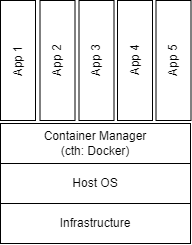
\includegraphics[width=.35\textwidth]{ContainerDiagram.png}
	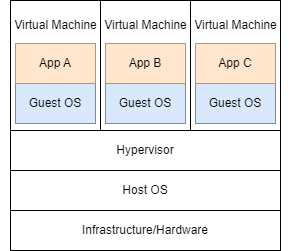
\includegraphics[width=.5\textwidth]{VirtualizationDiagram.png}
	\caption{Arsitektur Container vs Virtualization.}
	\label{fig:ContainerDiagram}
	\end{center}
\end{figure}

\section{Definisi}

\textbf{Container Architecture} merupakan sebuah konsep arsitektur yang dirancang untuk menjalankan aplikasi dalam container. Container Architecture memiliki beberapa tugas yaitu Isolasi, Portabilitas, Efisiensi, Deployment.

\textbf{Container} adalah metode menjalankan aplikasi yang memungkinkannya berjalan secara konsisten di berbagai lingkungan komputasi.\\ 
Secara sederhana, container dapat dianggap sebagai paket yang berisi semua elemen yang diperlukan untuk menjalankan aplikasi tertentu, seperti OS, library, config, dependencies, dan file penting lainnya yang dibutuhkan untuk menjalankan aplikasi tersebut.

\textbf{Docker} adalah platform open source untuk mengembangkan, menguji, dan mengimplementasikan aplikasi dalam container. 
Dalam konteks Docker, container adalah lingkungan terisolasi yang dapat berjalan di host yang sama tanpa pengaruh aplikasi atau sistem operasi lain yang berjalan di host yang sama. Container dapat dianggap sebagai paket yang berisi semua elemen yang diperlukan untuk menjalankan aplikasi tertentu, termasuk perangkat lunak, pustaka, konfigurasi, dan dependensi lainnya.

\textbf Alternatifnya {Kubernetes}, adalah platform open source untuk mengelola aplikasi dalam container yang dibuat oleh Google. Kubernetes memungkinkan pengguna untuk menjalankan, mengelola, dan mengotomatiskan penerapan aplikasi dalam container secara efisien.

\begin{figure}[h]
    \centering
    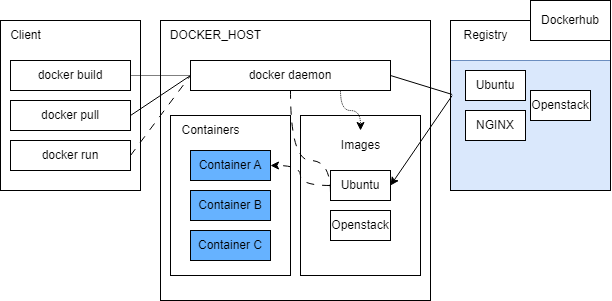
\includegraphics[width=\textwidth]{DockerDiagram.png}
    \caption{Diagram Docker.}
    \label{fig:ContainerDiagram}
\end{figure}

\textbf{Docker image}. Image disini bukan lah Image yang kita bayangkan (.jpg, .png, etc). Image pada Docker adalah sebuah template read-only atau cuplikan/snapshot berisikan instruksi untuk membuat container yang nantinya akan dipakai. Docker Image membuat Container untuk dijalankan di Docker Platform. Analoginya, Docker image itu seperti blueprint apartemen. 

\textbf{Docker Build}. Cara membuat Docker image adalah dengan membuat file Dockerfile (yaitu instruksi pembuatan imagenya) dan menggunakan "docker build" pada dockerfile tersebut. 

\textbf{Docker Pull} adalah perintah untuk mendownload/pull image docker dari registry(cth Dockerhub)

\textbf{Docker Registry} adalah sebuah repository berbagai docker images yang dibagikan oleh para developer.

\textbf {Docker Run} adalah perintah untuk menjalankan docker images dan membentuk Docker Container berdasarkan image yang dipilih.

\textbf {Docker Container} adalah instansi Container hasil dijalankannya image yang bisa distart, stop, restart, ataupun dihapus. Analoginya, inilah ruangan Kos apartemen hasil blueprint.

\textbf {Docker Daemon} adalah mesin/engine yang berjalan di mesin host dan memanage semua proses pada docker. Semua perintah perintah diatas seperti docker run itu dikirim ke docker daemon dan dijalankan.

\section{Kelebihan dan Kekurangan}
Berikut adalah kelebihan dan kekurangan docker:


\subsection{Kelebihan}
Keuntungan dari menggunakan docker adalah:
\begin{itemize}
\item Docker mempunyai konfigurasi yang \textit{sederhana} yang dapat disesuaikan dengan kebutuhan aplikasi yang sedang dikembangkan. Dengan menetapkan beberapa baris kode yang mendukung, docker mampu membuat lingkungannya sendiri yang terpisah dari lingkungan server utama.
\item Docker memiliki tingkat keamanan yang baik. Ia akan memastikan aplikasi yang sedang berjalan tidak dapat memengaruhi container \textit{(isolation)}. Selain itu, ia juga memiliki fitur keamanan \textit{pengaturan OS host mount} dengan akses \textit{read-only} sehingga konfigurasi yang tersedia tidak akan berubah sama sekali (kecuali pengguna memiliki akses penuh).
\item Docker dapat dijalankan pada beberapa platform cloud. Karena itu, pengguna dapat melakukan porting aplikasi dengan lebih mudah dan fleksibel. Selain itu, fitur-fitur docker juga dapat dijalankan pada berbagai sistem operasi, seperti Windows, Mac, dan Linux.
\item Docker mempunyai ukuran yang cukup ringan, dan lebih hemat sumber daya. Pengguna tidak membutuhkan memory storage atau overhead yang terlalu besar untuk menggunakannya.
\item Docker memiliki fitur debugging. Waktu yang dibutuhkannya juga tergolong cepat, yakni hanya sekitar satu menit saja untuk melakukan proses debug pada Sandbox.
\end{itemize}

\subsection{Kekurangan}
Konsekuensi dari menggunakan docker adalah sebagai berikut:
\begin{itemize}
\item Walaupun dapat digunakan pada berbagai macam OS, docker mempunyai kompatibilitas \textit{cross-platform} yang kurang fleksibel. Ketika sebuah aplikasi dirancang menggunakan Windows, pengguna memerlukan bantuan \textit{tools} eksternal untuk menjalankannya di Linux.
\item Secara garis besar, docker memiliki kekurangan fitur yang harus diakali pengguna dengan cara meng-install perangkat lunak eksternal apabila pengguna tidak ingin melakukan manajemen manual. Contohnya, docker tidak mempunyai dukungan untuk health-check, atau pemrograman ulang otomatis dari node yang tidak aktif.
\end{itemize}

\section{Contoh Kasus Penggunaan Container Architecture}

Biasanya, Container Architecture ergo Docker Container dibutuhkan dalam pembuatan dan deploy aplikasi yang terdiri dari beberapa komponen berbeda, seperti {aplikasi web} yang terdiri dari server web, database, dan layanan lainnya.

Dengan menggunakan Docker, kita dapat mengemas setiap komponen aplikasi ke dalam container yang terisolasi dan dapat dijalankan secara independen di berbagai lingkungan, seperti lingkungan pengembangan, pengujian, dan produksi. Container Docker memungkinkan pengembang untuk menjamin bahwa aplikasi yang mereka kembangkan dapat dijalankan dengan konsisten di seluruh lingkungan, sehingga mengurangi risiko terjadinya kesalahan dan masalah ketika aplikasi dideploy.

Tanpa container/docker, dalam pembuatan aplikasi kita biasanya harus install dan konfigurasi setiap komponen aplikasi secara manual di setiap environment, seperti environment pengembangan, pengujian, dan produksi. Ini bisa bermasalah ketika aplikasi dideploy di lingkungan yang berbeda, karena berbeda konfigurasi dan pengaturannya. 

\textbf{Contoh kasus}, misal ada sebuah aplikasi php yang sudah didevelop menggunakan php7, belum tentu aplikasi tersebut bisa dijalankan di komputer lain yang menjalankan php5. Dengan menggunakan docker, meskipun pada dasarnya komputernya menggunakan php5, namun image dan containernya sudah ada php7 jadinya tidak perlu konfigurasi ulang.

\section{Demo Container Architecture Menggunakan Docker}
Pada bagian ini Richwen akan mendemokan cara kerja docker. Codenya ada di folder code chapter 13.

aaaaa


\backmatter
\addcontentsline{toc}{chapter}{Daftar Pustaka}
%\bibliographystyle{splncs}
\bibliography{references}

\end{document}